\documentclass[12pt, a4paper, french]{thloria}
%\ThesisDraft

\newcommand{\TitreThese}{
Manipulation et refroidissement par �vaporation forc�e d'ensembles atomiques ultra-froids pour la production d'un jet intense dans le r�gime de d�g�n�rescence quantique : vers l'obtention d'un \textit{laser � atomes continu}}

\usepackage{ifthen}
\usepackage{ifpdf}

%\usepackage[pdftex]{thumbpdf}
\usepackage[pdftex]{graphicx} % pour l'incusion de graphiques


\graphicspath{{images/}}
%\setkeys{Gin}{width=\linewidth}

\usepackage[intlimits]{amsmath}
\usepackage{amssymb}
% pour des repr�sentation de vecteur sympa pour les physiciens
\usepackage{vector}
\usepackage{array}
\usepackage{slashbox}% pour couper une case de tableau en deux

% figures avec sous-figures et sous-captions:
\usepackage[subrefformat=subparens]{subfig}

% pour des r�f�rences en language naturel
\usepackage[english]{varioref} 

% pour des supers graphiques trop cool, mieux que PSTricks
\usepackage{tikz,tkz-fct,tkz-2d}
\usetikzlibrary{shapes,snakes,arrows,patterns}

\usepackage[np,autolanguage]{numprint}

\usepackage[autoplay, loop, poster]{animate} % pour animer des dessins

% texte sur des images
\usepackage[abs]{overpic}
\setlength\unitlength{1cm}

%%%%%%%%%%%%%%%%%%%%%%%%%%%%%%%%%%%%%%%%%%%%%%%%%%%%%%%
% Pour pouvoir avoir des fleche depuis le texte vers des formule par exemple:
% http://www.fauskes.net/pgftikzexamples/global-nodes/
%%%%%%%%%%%%%%%%%%%%%%%%%%%%%%%%%%%%%%%%%%%%%%%%%%%%%%%
% For every picture that defines or uses external nodes, you'll have to apply the 'remember picture' style. To avoid some typing, we'll apply the style to all pictures.
\tikzstyle{every picture}+=[remember picture] 
% By default all math in TikZ nodes are set in inline mode. Change this to displaystyle so that we don't get small fractions.
\everymath{\displaystyle}

% espace int�ligent pour la fin d'une nexcommand en text
\usepackage{xspace}

%gestion des unit� !
\usepackage[amssymb]{SIunits}
\usepackage{sistyle}
\SIstyle{German} 

\usepackage{picins}
\usepackage{fancybox}

\usepackage{movie15}
% hachurer du texte avec \sout{Texte � barrer}\xout{Texte � hachurer}\uwave{Texte � souligner par une vaguelette}
\usepackage[normalem]{ulem}


% pour ajouter localement une ligne � une page
% contient une commande pour checker si on est sur un page odd or even
\usepackage{addlines}
\usepackage{mparhack}

% Si on veut des mini-tables des matieres (utiliser minitoc-hyper en conjonction avec tulhypref) :
\ifpdf % le monde PDF
\usepackage[french]{minitoc-hyper}
\else % le monde DVI/PS
\usepackage[french]{minitoc}
\fi
%\renewcommand{\mtctitle}{dfgh}

% Liste notations
\usepackage[refpage,english,intoc]{nomencl}  %intoc rajoute une ligne dans la toc

%\usepackage{tocbibind}                     % toc,lotf,bib,index in toc
%\usepackage[numbers,sort&compress]{natbib} % Good [47] type referencing
%\usepackage{hypernat}                      % Makes natbibs s&c play w/ hyperref

\ifpdf % le monde PDF
%\usepackage{hyperref} % pour des r�f�rences cliquables
\usepackage[pdftex, colorlinks = true
%						, pdfstartview = FitH
%						, colorlinks=false,
						, linkcolor = black, citecolor = black, urlcolor = black, pdfpagelabels, pagebackref]{tulhypref}
\hypersetup{pdfauthor={Gael Reinaudi},
pdftitle={\TitreThese},
pdfsubject={Th�se de doctorat},
pdfkeywords={physique,quantique,laser,atome,d�g�n�rescence,froid,manipulation,atomique,refroidissement,�vaporation,jet}}
\else % le monde DVI/PS
\fi
% ********************************************************************
% get the links to the figures and tables right
%\RequirePackage[all]{hypcap} % to be loaded after hyperref package
% ********************************************************************
% setup the style of the backrefs from the bibliography
\newcommand{\backrefnotcitedstring}{\relax}%(Not cited.)
\newcommand{\backrefcitedsinglestring}[1]{Cit� � la page~#1.}
\newcommand{\backrefcitedmultistring}[1]{Cit� aux pages~#1.}
\RequirePackage[hyperpageref]{backref} % to be loaded after hyperref package
   \renewcommand{\backreftwosep}{ et~} % seperate 2 pages
   \renewcommand{\backreflastsep}{, et~} % seperate last of longer list
   \renewcommand*{\backref}[1]{}  % Disable standard
   \renewcommand*{\backrefalt}[4]{% Detailed backref
      \ifcase #1 %
         \backrefnotcitedstring%
      \or
         \backrefcitedsinglestring{#2}%
      \else
         \backrefcitedmultistring{#2}%
      \fi} 
% ********************************************************************

% Si l'on produit le PDF avec pdflatex, ceci remplace la plupart
% des polices EC par des polices CM, plus adaptees a la generation de PDF,
% car ayant des equivalents PS :
\usepackage{aeguill}
% Pour tout savoir sur les polices
% (cette ligne n'est pas necessaire au traitement du fichier)
%\usepackage[infoshow]{tracefnt}

% �vite les under-over full box...
%\usepackage[auto=false]{microtype} % 2010-05-27
%\usepackage{microtype}

\usepackage[latin1]{inputenc}
\usepackage{times}
\usepackage[T1]{fontenc}
\usepackage{lmodern}





% Pour publication EUE
\usepackage[top=20mm, bottom=20mm]%, left=20mm, right=20mm]
{geometry}
\SetRealMargins{20mm}{25mm}

\newcommand{\NoAnimationsInFigures}{1}
\newcommand{\FormatEUE}{1}

\newcommand{\IncludePartOne}{1}
\newcommand{\IncludePartTwo}{1}
\newcommand{\IncludePartThree}{1}
\newcommand{\IncludeAnnexe}{1}

\newcommand{\TitrePartieUn}{Production et �vaporation d'un \jatg}
\newcommand{\TitrePartieDeux}{Manipulation de \pats dilu�s}
\newcommand{\TitrePartieTrois}{Production, manipulation et caract�risation de \ns denses}

\newcommand{\TitreChapitreUn}{Dispositif exp�rimental, �vaporation d'un \jatg}
\newcommand{\TitreChapitreDeux}{�vaporation d'un \jat au contact d'une surface mat�rielle}
\newcommand{\TitreChapitreTrois}{R�flexion d'un \pat sur un \mimo}
\newcommand{\TitreChapitreQuatre}{Transport de \pats dans un train de pi�ges magn�tiques}
\newcommand{\TitreChapitreCinq}{Production et transport non-adiabatique de \ns denses dans un \pd}
\newcommand{\TitreChapitreSix}{Imagerie de \ns denses par absorption dans le r�gime de forte saturation}

\FrenchFootnotes

%%%%%%%%%%%%%%%%%%%%%%%%%%%%%%%%%%%%%%%%%%%%%%%%%%%%%%%%%%%%%%%%%%%%%%%%%%%%%%%%%%%%%%%%%%%%%%%%%%%%%%%%%%%%%%%%%%%%%%%%%%%%%%
%%%%%%%%%%%%%%%%%%%%%%%%%%%%%%%%%%%%%%%%%%%%%%%%%%%%%%%%%%%%%%%%%%%%%%%%%%%%%%%%%%%%%%%%%%%%%%%%%%%%%%%%%%%%%%%%%%%%%%%%%%%%%%
%%%%%%%%%%%%%%%%%%%%%%%%%%%%%%%%%%%%%%%%%%%%%%%%%%%%%%%%%%%%%%%%%%%%%%%%%%%%%%%%%%%%%%%%%%%%%%%%%%%%%%%%%%%%%%%%%%%%%%%%%%%%%%
%-------------------------------------------------------------------
%                             En-tetes
%-------------------------------------------------------------------

% Les en-tetes: quelques exemples
%\UppercaseHeadings 
%\UnderlineHeadings
%\newcommand\bfheadings[1]{{\bf #1}}
%\FormatHeadingsWith{\bfheadings}
%\FormatHeadingsWith{\uppercase}
%\FormatHeadingsWith{\underline}
\newcommand\upun[1]{\uppercase{\underline{\underline{#1}}}}
\FormatHeadingsWith\upun

\newcommand\itheadings[1]{\textit{#1}}
\FormatHeadingsWith{\itheadings}

% pour avoir un trait sous l'en-tete:
\setlength{\HeadRuleWidth}{0.4pt}



\NoChapterNumberInRef
\NoChapterPrefix

%%%%%%%%%%%%%%%%%%%%%%%%%%%%%%%%%%%%%%
\ResetFootnotesAtChapters
%%%%%%%%%%%%%%%%%%%%%%%%%%%%%%%%%%%%%%
\SetTocSpacing{1,25}
%-------------------------------------------------------------------
%                           Brouillons
%-------------------------------------------------------------------

% ceci ajoute une marque `brouillon' et la date
%\ThesisDraft

%-------------------------------------------------------------------
%                   Pour collecter un glossaire et un index
%-------------------------------------------------------------------

\makeglossary
\makeindex
%%%%%%%%%%%%%%%%%%%%%%%%%%%%%%%%%%%%%%%%%%%%%%%%%%%%%%%%%%%%%%%%%%%%%%%%%%%%%%%%%%%%%%%%%%%%%%%%%%%%%%%%%%%%%%%%%%%%%%%%%%%%%%
%%%%%%%%%%%%%%%%%%%%%%%%%%%%%%%%%%%%%%%%%%%%%%%%%%%%%%%%%%%%%%%%%%%%%%%%%%%%%%%%%%%%%%%%%%%%%%%%%%%%%%%%%%%%%%%%%%%%%%%%%%%%%%
%%%%%%%%%%%%%%%%%%%%%%%%%%%%%%%%%%%%%%%%%%%%%%%%%%%%%%%%%%%%%%%%%%%%%%%%%%%%%%%%%%%%%%%%%%%%%%%%%%%%%%%%%%%%%%%%%%%%%%%%%%%%%%



\begin{document}

\newcommand\FaitNomenclature{1}
\newcommand\FaitNomEnMarge{1}

\renewcommand{\emph}[1]{\textbf{\textit{{#1}}}}
\providecommand{\enquote}[1]{``#1''}

\newcommand{\termetech}[1]{\textit{{#1}}}
\newcommand{\nomofficiel}[1]{\textit{{#1}}}
\newcommand{\sotosay}[1]{\enquote{\textit{{#1}}}}
\newcommand{\parole}[1]{\og\textit{{#1}}\fg}

\newenvironment{itemizel}%
   {\begin{itemize}}{\end{itemize}\vspace*{1.5ex}}%

\newenvironment{ditemize}%
%   {\begin{list}%
%   {$\bullet$}{}%
%   }{\end{list}}%
   {\begin{itemize}}{\end{itemize}}%

% ************************************************************************
\newcommand{\casse}{\pagebreak}
% ************************************************************************
\newcommand{\bfig}{\begin{GaelFigure}}
\newcommand{\bfigs}{\bfig\RemonteUnPeuFig}
\newcommand{\bfigss}{\bfigs\RemonteUnPeuFig}
\newcommand{\bfigsss}{\bfigss\RemonteUnPeuFig}
\newcommand{\bfighs}{\bfigh\RemonteUnPeuFig}
\newcommand{\bfighss}{\bfighs\RemonteUnPeuFig}
\newcommand{\bfighsss}{\bfighss\RemonteUnPeuFig}
\newcommand{\CaptionFigs}[1]{\RemonteUnPeuFig \CaptionFig{#1}}
\newcommand{\CaptionFigss}[1]{\RemonteUnPeuFig \CaptionFigs{#1}}
\newcommand{\CaptionFigsss}[1]{\RemonteUnPeuFig \CaptionFigss{#1}}
\newcommand{\CaptionFigssss}[1]{\RemonteUnPeuFig \CaptionFigsss{#1}}

\newcommand{\efig}{\end{GaelFigure}}
\newcommand{\bfigh}{\begin{GaelFigureh}}
\newcommand{\efigh}{\end{GaelFigureh}}

\newcommand{\inlinefigr}[1]{\parpic[r,s]{{#1}}}
\newcommand{\inlinefigl}[1]{\parpic[l,s]{{#1}}}
\newcommand{\inlinefig}[1]{\inlinefigr{#1}}

% Pour enlever toutes les figures !
%\renewcommand{\includegraphics}[2][]{}\renewcommand{\animategraphics}[5][]{}
   
% Des notes pour donner des points de repere dans les cahier de labo.
% A commenter pour la version publique
\newcommand{\Cahier}[1]{%
%{\color{red}{CAHIER,PAGE #1}}%
}
% Des notes pour Gael.
% A commenter pour la version publique
\newcommand{\NoteGael}[1]{%
%{\color{magenta}{NOTE GAEL : \noindent #1 }}%
}
% Supprime de la version compil�e ce qu'il y a en argument
\newcommand{\EnFaitNon}[1]{}

% Les copi�s coll�s de TTL au cas o�
\newcommand{\dixit}[1]{#1}

% Les r�f�rences sans page
\newcommand{\nref}[1]{\ref{#1}}

\newcommand{\ttfrac}[2]{{{#1} / {#2}}}
%\newcommand{\ttfrac}[2]{{\sfrac{#1}{#2}}}

\newcommand{\AnimateOnline}{{(Animation en ligne) }}

%%%%%%%%%%%%%%%%%%%%%%%%%%%%%%%%%%%%%%%%%%%%%%%%%%%%%%%
% TIKZ : Pour pouvoir avoir des supers jolies boites avec du texte et des formule exemple:
% http://www.fauskes.net/pgftikzexamples/boxes-with-text-and-math/
%%%%%%%%%%%%%%%%%%%%%%%%%%%%%%%%%%%%%%%%%%%%%%%%%%%%%%%
\newcommand{\nResultat}[1]{#1}
\newcommand{\nRemarque}[1]{#1}
\newcommand{\nRemarqueTitre}[2]{\subsubsection{#1}#2}
\newcommand{\nnRemarque}[1]{}
\newcommand{\nnRemarqueTitre}[2]{}
%%%%%%%%%%%%%%%%%%%%%%%%%%%%%%%%%%%%%%%%%%%%%%%%%%%%%%%
% Boite d'Intuition
% Define box and box title style
\tikzstyle{IntuitionBox}=[draw=black, fill=green!05, very thick, 
rectangle, rounded corners, inner sep=10pt, inner ysep=13pt]
\tikzstyle{IntuitionTitre}=[draw=black, very thick, fill=white, text=black]
%\newcommand{\Intuition}[1]{%
%\begin{center}\begin{tikzpicture}
%\node [IntuitionBox] (box){%
%	\begin{minipage}{0.85\textwidth}%
%		{\color{black}{#1}%
%		\newpage}%
%		\vspace{-5pt}%
%	\end{minipage}};%
%\node[IntuitionTitre, anchor=center] at (box.north)
%{De mani�re qualitative...};
%\end{tikzpicture}\end{center}
%}

%%%%%%%%%%%%%%%%%%%%%%%%%%%%%%%%%%%%%%%%%%%%%%%%%%%%%%%
% Boite de Resultat important
\tikzstyle{ResultatBox}=[draw=red, fill=red!5, very thick,
    rectangle, rounded corners, inner sep=10pt, inner ysep=10pt]
\tikzstyle{ResultatTitre}=[fill=red, text=black]
\newcommand{\Resultat}[1]{%
\begin{center}\begin{tikzpicture}%
\node [ResultatBox] (box){%
	\begin{minipage}{0.85\textwidth}%
		{\color{black}{#1}%
		\newpage}%
	\end{minipage}};%
%\node[ResultatTitre, right=10pt] at (box.north west) {R�sultat};
\end{tikzpicture}\end{center}
}

%%%%%%%%%%%%%%%%%%%%%%%%%%%%%%%%%%%%%%%%%%%%%%%%%%%%%%%
% Boite d'Application num�rique
\tikzstyle{ApplicationNumeriqueBox}=[draw=black!20!green, fill=green!2, thick,
    rectangle, inner sep=10pt, inner ysep=13pt]
\tikzstyle{ApplicationNumeriqueTitre}=[draw=black!20!green, thick
, fill=white, text=black]
\newcommand{\ApplicationNumerique}[1]{%
\begin{center}\begin{tikzpicture}
\node [ApplicationNumeriqueBox] (box){%
	\begin{minipage}{0.85\textwidth}%
		{\color{black}{#1}%
		\newpage}%
		\vspace{-5pt}%
	\end{minipage}};%
\node[ApplicationNumeriqueTitre, right=10pt] at (box.north west)%
{Application num�rique};
\end{tikzpicture}\end{center}
}
\newcommand{\ApplicationNumeriqueTitre}[2]{%
\begin{center}\begin{tikzpicture}
\node [ApplicationNumeriqueBox] (box){%
	\begin{minipage}{0.85\textwidth}%
		{\color{black}{#2}%
		\newpage}%
		\vspace{-5pt}%
	\end{minipage}};%
\node[ApplicationNumeriqueTitre, right=10pt] at (box.north west)%
{Application num�rique : #1};
\end{tikzpicture}\end{center}
}

%%%%%%%%%%%%%%%%%%%%%%%%%%%%%%%%%%%%%%%%%%%%%%%%%%%%%%%
% Boite de Remarque
\tikzstyle{RemarqueBox}=[fill=blue!5, 
rectangle, inner sep=5pt, inner ysep=5pt]
\tikzstyle{RemarqueTitre}=[draw=white, thick, fill=white, text=black]
\tikzstyle{RemarqueLigne}=[color=blue
]%, very thick, cap=round]
\newcommand{\Remarque}[1]{%
\begin{center}\begin{tikzpicture}
\node [RemarqueBox, below right] (box)
{%
	\begin{minipage}{0.85\textwidth}%
		{\color{black}{#1}%
		\newpage}%
	\end{minipage}%
};
\node[RemarqueTitre, above right] at (box.north west) {Remarque};
\draw[RemarqueLigne] (box.north west)++(0,0.6)--(box.south west);
\draw[RemarqueLigne] (box.north west)--++(2,0);
\draw (box.south west)++(-1.5pt,0)--(-1.5pt,0.6);
%\draw[very thick] (box.north east)--(box.south east);
\end{tikzpicture}\end{center}
}
\newcommand{\RemarqueTitre}[2]{%
\begin{center}\begin{tikzpicture}
\node [RemarqueBox, below right] (box)
{%
	\begin{minipage}{0.85\textwidth}%
		{\color{black}{#2}%
		\newpage}%
	\end{minipage}%
};
\node[RemarqueTitre, above right] at (box.north west) {Remarque : {\textbf{#1}}};
\draw[RemarqueLigne] (box.north west)++(0,0.6)--(box.south west);
\draw[RemarqueLigne] (box.north west)--++(2,0);
\draw (box.south west)++(-1.5pt,0)--(-1.5pt,0.6);
\end{tikzpicture}\end{center}%
}
%%%%%%%%%%%%%%%%%%%%%%%%%%%%%%%%%%%%%%%%%%%%%%%%%%%%%%%%%%%%%%%%%%%%%%%%%%%%
%%%%%%%%%%%%%%%%%%%%%%%%%%%%%%%%%%%%%%%%%%%%%%%%%%%%%%%%%%%%%%%%%%%%%%%%%%%%
%%%%%%%%%%%%%%%%%%%%%%%%%%%%%%%%%%%%%%%%%%%%%%%%%%%%%%%%%%%%%%%%%%%%%%%%%%%%
%%%%%%%%%%%%%%%%%%%%%%%%%%%%%%%%%%%%%%%%%%%%%%%%%%%%%%%%%%%%%%%%%%%%%%%%%%%%
%%%%%%%%%%%%%%%%%%%%%%%%%%%%%%%%%%%%%%%%%%%%%%%%%%%%%%%%%%%%%%%%%%%%%%%%%%%%
\newcommand{\finformule}{\vspace{-3ex}}
\newcommand{\ff}{\finformule}
\newcommand{\RemonteUnPeuFig}{\vspace{-.2cm}}
\newcommand{\RemonteUneLigne}{\vspace{-3ex}}
\newcommand{\AjouteLigne}{\enlargethispage{1\baselineskip}}
\newcommand{\RetireLigne}{\enlargethispage{-1\baselineskip}}

\newenvironment{fminipage}{%
\begin{Sbox}\begin{minipage}}
{%
\end{minipage}\end{Sbox}
\shadowbox{\TheSbox}}

% Les figures � gael******************************************************
\newcommand{\MinipageWidth}{15cm}
\newcommand{\CaptionWidth}{14.6cm}
\newcommand{\CaptionMargin}{0.2cm}
\newcommand{\FigWidth}{14.5cm}
\newcommand{\FigWidthSansCm}{14.5}
\newcommand{\CaptionFig}[1]{\caption{\small{#1}}}
\newcommand{\CaptionTocCaptionFig}[2]{\caption[#1]{\small{#2}}}
\newcommand{\SansCaption}{\vspace{-0.24cm}}
% Les figures � gael******************************************************
\newenvironment{GaelFigure}[1][\MinipageWidth]{%
\begin{figure}[htbp]
\centering
\begin{fminipage}{#1}
\centering
\vspace{\CaptionMargin}
\pgfmathqparse{#1-\CaptionMargin-\CaptionMargin}
\begin{minipage}{\pgfmathresult pt}
\centering
}{%
\end{minipage}
\end{fminipage}
\end{figure}}
% Les figures � gael******************************************************
\newenvironment{GaelFigureh}[1][\MinipageWidth]{%
\begin{figure}[!ht]
\centering
\begin{fminipage}{#1}
\centering
\vspace{\CaptionMargin}
\pgfmathqparse{#1-\CaptionMargin-\CaptionMargin}
\begin{minipage}{\pgfmathresult pt}
\centering
}{%
\end{minipage}
\end{fminipage}
\end{figure}}

% ************************************************************************

%%%%%%%%%%%%%%%%%%%%%%%%%%%%%%%%%%%%%%%%%%%%%%%%%%%%
%% Pour faire des supers fleche d'hilight entre texte et �quation %%
%% http://www.fauskes.net/pgftikzexamples/global-nodes/
%% On d�finit un bout de fleche, et un d�part de fleche, puis on dit de faire les fleches....

\newcommand{\DepartHighlightColor}[2]%
{\tikz[baseline=(From#1.base)] {\node[fill=#1!10](From#1){#2};}}
%{#2}
\newcommand{\ArriveeHiglightColor}[2]%
{\tikz[baseline=(To#1.base)] {\node[fill=#1!10](To#1){#2};}}
%{#2}

\newcommand{\DepartHighlightColorMath}[2]{\DepartHighlightColor{#1}{\ensuremath{#2}}}%
\newcommand{\ArriveeHiglightColorMath}[2]{\ArriveeHiglightColor{#1}{\ensuremath{#2}}}%

\newcommand{\MakeFlecheHighlightColor}[1]%
{ \begin{tikzpicture}
[overlay]\path[->,opacity=0.5](From#1)edge%[bend left]
(To#1);
\end{tikzpicture}}
%{}

%%%%%%%%%%%%%%%%%%%%%%%%%%%%%%%%%%%%%%%%%%%%%%%%%%%%%%%%%%%%%%
%%%%%%%%% New commande pour le  texte%%%%%%%%%%%%%%%%%%%%%%%%%%%
\newcommand{\dgo}{David Gu�ry-Odelin\xspace}
\newcommand{\exatf}{exp�rience d'atome froids\xspace}
\newcommand{\exatfs}{exp�riences d'atome froids\xspace}
\newcommand{\thiq}{thermique\xspace}
\newcommand{\thdy}{thermodynamique\xspace}
\newcommand{\eqthdy}{�quilibre \thdy}
\newcommand{\reflab}{r�f�rentiel du laboratoire\xspace}
\newcommand{\refmir}{r�f�rentiel du miroir\xspace}
\newcommand{\dB}{de Broglie\xspace}

\newcommand{\tf}{transform�e de Fourier\xspace}

\newcommand{\rf}{radio-fr�quence\xspace}
\newcommand{\rfs}{{\rf}{s}\xspace}
\newcommand{\crf}{couteau \rf}
\newcommand{\hf}{hyperfin\xspace}
\newcommand{\hfs}{{\hf}{s}\xspace}
\newcommand{\sn}{sous-niveau\xspace}
\newcommand{\snx}{\sn{x}\xspace}
\newcommand{\snZ}{\sn Zeeman\xspace}
\newcommand{\snZs}{\snx Zeeman\xspace}
\newcommand{\snhf}{{\sn} \hf}
\newcommand{\snhfs}{{\snx} \hfs}

\newcommand{\ZS}{ralentisseur � effet Zeeman\xspace}

\newcommand{\rb}{rubidium\xspace}
\newcommand{\Rb}{$^{87}$Rb\xspace}
\newcommand{\RbCinq}{$^{85}$Rb\xspace}
\newcommand{\bec}{condensat de Bose-Einstein\xspace}
\newcommand{\becc}{condensat\xspace}
\newcommand{\beccs}{{\becc}s\xspace}
\newcommand{\becs}{condensats de Bose-Einstein\xspace}
\newcommand{\cbe}{condensation de Bose-Einstein\xspace}
\newcommand{\condbe}{\cbe}
\newcommand{\lat}{{laser � atomes}\xspace}
\newcommand{\lats}{{lasers � atomes}\xspace}
\newcommand{\rdq}{r�gime de d�g�n�rescence quantique\xspace}

\newcommand{\seqexp}{s�quence exp�rimentale\xspace}
\newcommand{\seqexps}{s�quences exp�rimentales\xspace}
\newcommand{\cdm}{centre de masse\xspace}

\newcommand{\ud}{unidimensionnel\xspace}
\newcommand{\ude}{unidimensionnelle\xspace}
\newcommand{\uds}{unidimensionnels\xspace}
\newcommand{\bd}{bidimensionnel\xspace}
\newcommand{\bde}{bidimensionnelle\xspace}
\newcommand{\bds}{bidimensionnels\xspace}
\newcommand{\td}{tridimensionnel\xspace}
\newcommand{\tde}{tridimensionnelle\xspace}
\newcommand{\tds}{tridimensionnels\xspace}

\newcommand{\reth}{rethermalisation\xspace}
\newcommand{\rether}{rethermaliser\xspace}
\newcommand{\cad}{c'est-�-dire\xspace}
%\newcommand{\Cad}{C'est-�-dire\xspace}
\newcommand{\ie}{i.\,e.\xspace}
\newcommand{\eg}{e.\,g.\xspace}
\newcommand{\etal}{\textit{et al.}\xspace}

\newcommand{\lsonde}{laser sonde\xspace}
\newcommand{\p}{paquet\xspace}
\newcommand{\ps}{paquets\xspace}
\newcommand{\pss}{\ps successifs\xspace}
\newcommand{\pat}{\p atomique\xspace}
\newcommand{\pats}{\ps atomiques\xspace}
\newcommand{\patss}{\pats successifs\xspace}
\newcommand{\n}{nuage\xspace}
\newcommand{\ns}{nuages\xspace}
\newcommand{\nat}{\n atomique\xspace}
\newcommand{\nats}{\ns atomiques\xspace}
\newcommand{\uf}{ultra-froid\xspace}
\newcommand{\ufs}{ultra-froids\xspace}
\newcommand{\natuf}{{\nat} \uf}
\newcommand{\natufs}{{\nats} \ufs}
\newcommand{\aufs}{atomes \ufs}
\newcommand{\patuf}{{\pat} \uf}
\newcommand{\patufs}{{\pats} \ufs}

\newcommand{\edp}{espace des phases\xspace}
\newcommand{\edpup}{espace des phases � une particule\xspace}
\newcommand{\edpNp}{espace des phases � $N$ particules\xspace}
\newcommand{\ddedp}{densit� dans l'espace des phases\xspace}
\newcommand{\ddedpup}{densit� dans l'espace des phases � une particule\xspace}
\newcommand{\dmdedp}{densit� moyenne dans l'espace des phases\xspace}
\newcommand{\dmdedpup}{densit� moyenne dans l'espace des phases � une particule\xspace}
\newcommand{\ddedpNp}{densit� dans l'espace des phases � $N$ particules\xspace}

\newcommand{\fdd}{fonction de distribution\xspace}
\newcommand{\fdddedpup}{\fdd dans l'\edpup}
\newcommand{\fdddedpNp}{\fdd dans l'\edpNp}

\newcommand{\tlin}{transverse lin�aire\xspace}
\newcommand{\thar}{transverse harmonique\xspace}
\newcommand{\thyp}{transverse hyperbolique\xspace}
\newcommand{\pma}{potentiel magn�tique\xspace}
\newcommand{\ptlin}{potentiel \tlin}
\newcommand{\pthar}{potentiel \thar}
\newcommand{\pthyp}{potentiel \thyp}
\newcommand{\ctlin}{confinement \tlin}
\newcommand{\cthar}{confinement \thar}
\newcommand{\cthyp}{confinement \thyp}
\newcommand{\pp}{potentiel de pi�geage\xspace}
\newcommand{\pphar}{\pp harmonique\xspace}
\newcommand{\pplor}{\pp lorentzien\xspace}
\newcommand{\ppgau}{\pp gaussien\xspace}
\newcommand{\pc}{potentiel de confinement\xspace}
\newcommand{\pct}{\pc transverse\xspace}
\newcommand{\pcl}{\pc longitudinal\xspace}
%\newcommand{\ppt}{\pp transverse\xspace}
\newcommand{\ppt}{\pct}
%\newcommand{\ppl}{\pp longitudinal\xspace}
\newcommand{\ppl}{\pcl}
\newcommand{\ppllor}{\pp longitudinal lorentzien\xspace}
\newcommand{\pctlin}{potentiel de \ctlin}
\newcommand{\pcthar}{potentiel de \cthar}
\newcommand{\pcthyp}{potentiel de \cthyp}
\newcommand{\pptlin}{\pctlin}
\newcommand{\ppthar}{\pcthar}
\newcommand{\ppthyp}{\pcthyp}

\newcommand{\bapot}{barri�re de potentiel\xspace}
\newcommand{\bapots}{barri�res de potentiel\xspace}

\newcommand{\spfi}{spectre de filtrage\xspace}
\newcommand{\spfirf}{spectre de filtrage \rf}
\newcommand{\spfirfs}{spectres de filtrage \rfs}
\newcommand{\firf}{filtrage \rf}
\newcommand{\fisp}{filtrage spatial\xspace}
\newcommand{\fispse}{\fisp s�lectif\xspace}
\newcommand{\spfihf}{spectre de filtrage \hf}

\newcommand{\colel}{collision �lastique\xspace}
\newcommand{\colels}{collisions �lastiques\xspace}
\newcommand{\tcoli}{taux de collisions\xspace}
\newcommand{\tcolel}{taux de \colels}
\newcommand{\Ncolel}{nombre de \colels}

\newcommand{\thLi}{th�or�me de Liouville\xspace}

\newcommand{\uv}{ultra-vide\xspace}
\newcommand{\setup}{dispositif exp�rimental\xspace}
\newcommand{\setups}{dispositifs exp�rimentaux\xspace}
\newcommand{\setupp}{montage exp�rimental\xspace}
\newcommand{\tof}{temps de vol\xspace}
\newcommand{\aom}{modulateur acousto-optique\xspace}

\newcommand{\dispvitlong}{dispersion de vitesse longitudinale\xspace}
\newcommand{\distvitlong}{distribution de vitesse longitudinale\xspace}

\newcommand{\pmo}{pi�ge magn�to-optique\xspace}
\newcommand{\pmobd}{{\pmo} \bd}
\newcommand{\pmos}{pi�ges magn�to-optiques\xspace}

\newcommand{\tempt}{temp�rature transverse\xspace}
\newcommand{\templong}{temp�rature longitudinale\xspace}
\newcommand{\vitlong}{vitesse longitudinale\xspace}
\newcommand{\vitlongs}{vitesses longitudinales\xspace}

\newcommand{\chm}{champ magn�tique\xspace}
\newcommand{\chms}{champs magn�tiques\xspace}
\newcommand{\che}{champ �lectrique\xspace}
\newcommand{\ches}{champs �lectriques\xspace}
\newcommand{\di}{dip�le induit\xspace}
\newcommand{\da}{dip�le atomique\xspace}
\newcommand{\gchm}{gradient de \chm}
\newcommand{\gtchm}{gradient transverse de \chm}
\newcommand{\gm}{guide magn�tique\xspace}
\newcommand{\qp}{quadrupolaire\xspace}
\newcommand{\qpdd}{\qp � deux dimensions\xspace}
\newcommand{\pqp}{pi�ge \qp}
\newcommand{\pmqp}{pi�ge magn�tique \qp}
\newcommand{\pqps}{{pi�ges \qp}{s}\xspace}
\newcommand{\pmqps}{{pi�ges magn�tiques \qp}{s}\xspace}
\newcommand{\IP}{Ioffe-Pritchard\xspace}
\newcommand{\pIP}{pi�ge de \IP}
\newcommand{\pIPs}{pi�ges de \IP}
\newcommand{\tpqp}{train de \pqps}
\newcommand{\tpqpb}{{\tpqp} \bds}
\newcommand{\tpqpt}{\tpqp tridimensionnels\xspace}
\newcommand{\tpIP}{train de \pIPs}

\newcommand{\secpent}{section pentue\xspace}

\newcommand{\mi}{miroir\xspace}
\newcommand{\mis}{{\mi}s\xspace}
\newcommand{\mimo}{miroir mobile\xspace}
\newcommand{\techmimo}{technique du \mimo}
\newcommand{\mima}{miroir magn�tique\xspace}
\newcommand{\mimamo}{miroir magn�tique mobile\xspace}

\newcommand{\fat}{flux atomique\xspace}
\newcommand{\fats}{{\fat}{s}\xspace}
\newcommand{\dat}{densit� atomique\xspace}
\newcommand{\dats}{densit�s atomiques\xspace}
\newcommand{\datlin}{densit� lin�ique d'atomes\xspace}
\newcommand{\dcol}{densit� colonne\xspace}

\newcommand{\evap}{�vaporation forc�e\xspace}
\newcommand{\rpe}{refroidissement par �vaporation\xspace}
\newcommand{\rpef}{refroidissement par \evap}

\newcommand{\ma}{magn�tique\xspace}
\renewcommand{\j}{jet\xspace}
\newcommand{\jat}{jet atomique\xspace}
\newcommand{\jaf}{jet d'atomes froids\xspace}
\newcommand{\jmg}{jet magn�tiquement guid�\xspace}
\newcommand{\jgm}{jet guid� magn�tiquement\xspace}
\newcommand{\jatg}{\jat guid�\xspace}
\newcommand{\jatgm}{\jatg magn�tiquement\xspace}
\newcommand{\jatmg}{\jat magn�tiquement guid�\xspace}
\newcommand{\jatuf}{{\jat} \uf}
\newcommand{\mg}{magn�tiquement guid�\xspace}

\newcommand{\conv}{convoyeur\xspace}
\newcommand{\couconv}{courroie du \conv}
\newcommand{\scc}{site de la \couconv}
\newcommand{\sccs}{\scc{s}}


%%%%%%%%%%%%%%%%%%%%%%%%%%%%%%%%%%%%%%%%%%%%%%%%%%%%%%%%%%%%%%%%%%%%%
\newcommand{\intsat}{intensit� de saturation\xspace}
\newcommand{\lintsat}{l'\intsat}
\newcommand{\intsateff}{\intsat effective\xspace}
\newcommand{\popuexcit}{population de l'�tat excit�\xspace}
\newcommand{\EBO}{�quations de Bloch optiques\xspace}

\newcommand{\ipf}{imagerie par fluorescence\xspace}
\newcommand{\Ipf}{Imagerie par fluorescence\xspace}
\newcommand{\ipa}{imagerie par absorption\xspace}
\newcommand{\Ipa}{Imagerie par absorption\xspace}
\newcommand{\ipafas}{imagerie par absorption faiblement saturante\xspace}
\newcommand{\ipafos}{imagerie par absorption fortement saturante\xspace}
\newcommand{\ipadrfs}{imagerie par absorption dans le r�gime de forte saturation\xspace}
\newcommand{\pro}{profondeur optique\xspace}
\newcommand{\pros}{profondeurs optiques\xspace}
\renewcommand{\do}{densit� optique\xspace}
\newcommand{\dos}{densit�s optiques\xspace}

\newcommand{\seff}{section efficace\xspace}
\newcommand{\seffeff}{\seff effective\xspace}
\newcommand{\seffabs}{\seff d'absorption\xspace}

\newcommand{\pdc}{param�tre de correction\xspace}

\newcommand{\pdec}{pi�ce de c�ramique\xspace}
\newcommand{\pdecs}{pi�ces de c�ramique\xspace}

\newcommand{\tp}{train de pi�ges\xspace}
\newcommand{\tpm}{\tp magn�tiques\xspace}


%%%%%%%%%%%%%%%%%%%%%%%%%%%%%%%%%%%%%%%%%%%%%%%%%%%%%%%%%%%%%%%%%%%%%%%%%%%%%%%%%
\newcommand{\dga}{D�l�gation G�n�rale pour l'Armement (DGA)\xspace}

\newcommand{\fd}{force dipolaire\xspace}
\newcommand{\fds}{forces dipolaires\xspace}
\newcommand{\pd}{pi�ge dipolaire\xspace}
\newcommand{\pdd}{pi�ge optique\xspace}
\newcommand{\pds}{pi�ges dipolaires\xspace}
\newcommand{\tna}{transport non-adiabatique\xspace}
\newcommand{\yb}{ytterbium\xspace}
\newcommand{\lyb}{laser \yb}
\newcommand{\ldp}{laser de puissance\xspace}
\newcommand{\ldps}{lasers de puissance\xspace}
\newcommand{\fl}{faisceau laser\xspace}
\newcommand{\fld}{faisceau dipolaire\xspace}
\newcommand{\fls}{faisceaux lasers\xspace}
\newcommand{\flp}{\fl de puissance\xspace}
\newcommand{\lo}{longueur d'onde\xspace}
\newcommand{\los}{longueurs d'onde\xspace}
\newcommand{\waist}{\termetech{waist}\xspace}
\newcommand{\waists}{\termetech{waists}\xspace}
\newcommand{\ldr}{longueur de Rayleigh\xspace}
\newcommand{\pacc}{profil d'acc�l�ration\xspace}
\newcommand{\paccs}{profils d'acc�l�ration\xspace}
\newcommand{\paccn}{profil normalis� d'acc�l�ration\xspace}
\newcommand{\BH}{Blackman-Harris\xspace}
\newcommand{\pBH}{profil de \BH}
\newcommand{\pn}{profil normalis�\xspace}
\newcommand{\pvit}{profil de vitesse\xspace}

\newcommand{\confa}{configuration~(a)\xspace}
\newcommand{\confb}{configuration~(b)\xspace}
\newcommand{\confab}{configurations~(a) et~(b)\xspace}

%%%%%%%%%%%%%%%%%%%%%%%%%%%%%%%%%%%%%%%%%%%%%%%%%%%%%%%%%%%%%%%%%%%%%%%%%%%%%%%%%%%%%%%
%%%%%%%%% New commande pour les math %%%%%%%%%%%%%%%%%%%%%%%%%%%%%%%%%%%%%%%%%%%%%%%%%%
\newcommand{\LO}{{\lambda}}%_{\rm 0}}}
\newcommand{\Irz}{I(r,z)}
\newcommand{\temzz}{{TEM$_{00}$}\xspace}
\newcommand{\wzero}{{w_0}}
\newcommand{\zR}{{z_{\rm R}}}
\newcommand{\wz}{{w(z)}}
\newcommand{\wzexpr}{\wzero\,\sqrt{1+ \left( \frac{z}{\zR} \right)^2 }}
\newcommand{\zRexpr}{{\pi\,\frac{\wzero^2}{\LO}}}

\newcommand{\Udip}{{U_{\rm dip}}}
\newcommand{\Udiph}{{U_{\rm h}}}
\newcommand{\Udiphxyz}{{U_{\rm h}\xyz}}
\newcommand{\Udipxyz}{{U_{\rm dip}\xyz}}
\newcommand{\Uprof}{{{U_0}}}
\newcommand{\Pmin}{{P_{\rm min}}}
\newcommand{\Ptrans}{{P_{\rm f}}}
\newcommand{\desacU}{{\Delta_{_{1}}}}
\newcommand{\desacD}{{\Delta_{_{2}}}}
\newcommand{\deseffcarre}{{\Delta_{_{12}}^{\hphantom{1}2}}}
\newcommand{\Gammadif}{{\Gamma_{\rm dif}}}
\newcommand{\dT}{{\Derive{T}{t}}}
\newcommand{\tdT}{{\tDerive{T}{t}}}

\newcommand{\PulsTrans}{{\omega_{r}}}
\newcommand{\PulsLong}{{\omega_{z}}}
\newcommand{\Uh}{{U_{\rm h}}}
\newcommand{\zc}{{z_{\rm c}}}
%\newcommand{\dzc}{{\stackrel{\centerdot}{\zc}}}
\newcommand{\dzc}{{\dot{\zc}}}
%\newcommand{\ddzc}{{\stackrel{\centerdot\centerdot}{\zc}}}
\newcommand{\ddzc}{{\ddot{\zc}}}
\newcommand{\dzct}{{\dzc(t)}}
\newcommand{\ddzct}{{\ddzc(t)}}
\newcommand{\ddzcn}{{\widehat{a}}}
\newcommand{\tadim}{{u}}
\newcommand{\ddzcnv}{{\ddzcn(\tadim)}}
\newcommand{\zct}{{\zc(t)}}
\newcommand{\tfin}{{T_{\rm f}}}
\newcommand{\Fe}{{F_{\rm e}}}
\newcommand{\zp}{{\tilde{z}}}
\newcommand{\vp}{{\tilde{v}}}
\newcommand{\zpt}{{\zp(t)}}
\newcommand{\vpt}{{\vp(t)}}
\newcommand{\PulsUh}{{\omega}}
\newcommand{\Aosc}{{\mathcal{A}}}
\newcommand{\AccZc}{A_{\rm m}}
\newcommand{\VitZc}{{V_{\rm m}}}
\newcommand{\DistZc}{{D}}
\newcommand{\PulsLongLor}{{\omega_{z}^{\rm lor}}}
\newcommand{\zmaxTraj}{{z_{\rm m}}}

\newcommand{\OperR}{{\mathbf{\widehat{R}}}}
\newcommand{\OperE}{{\mathbf{\widehat{E}}}}
\newcommand{\OperP}{{\mathbf{\widehat{d}}}}
\newcommand{\Evect}{{\Vecteur{E}}}
\newcommand{\Pvect}{{\Vecteur{d}}}
\newcommand{\Eampl}{{\widetilde{E}}}
\newcommand{\Pampl}{{\widetilde{d}}}
\newcommand{\Polarisation}{{\Vecteur{\epsilon_{_{\rm L}}}}}
\newcommand{\Vcav}{{V_{\rm c}}}
\newcommand{\Nph}{N}%{{N_{\rm ph}}}

\newcommand{\Ener}{{\mathcal{E}}}
\newcommand{\VAL}{{\mathbf{\widehat{V}_{\rm AL}}}}
\newcommand{\EAL}{{\mathcal{\Ener}_{\rm AL}}}
\newcommand{\omegaHF}{{\omega_{\rm hf}}}
\newcommand{\AiN}{{{A_i, \Nph}}}
\newcommand{\AjN}{{{A_j, \Nph'}}}
%\newcommand{\AjNpm}{{{A_j, \Nph\pm1}}}
\newcommand{\EcartMini}{{\Delta\Ener_{ij}}}
\newcommand{\Eneri}{{\Ener_{i}}}
\newcommand{\Enerj}{{\Ener_{j}}}
\newcommand{\Deltaij}{{\omega_{ij}}}
\newcommand{\EneriN}{{\Ener_{i\Nph}}}
\newcommand{\EnerjN}{{\Ener_{j\Nph'}}}
\newcommand{\PropUI}{\zeta}
\newcommand{\polarindice}{{q}}



\renewcommand{\unit}[1]{\ERREUR}
\newcommand{\val}[1]{{\num{#1}}}
\newcommand{\valpm}[2]{{\val{#1}\pm\val{#2}}}
\newcommand{\SiPlusOuMoins}[3]{{\val{#1}\pm\SI{#2}{#3}}}
\newcommand{\atparsec}[1]{\SI{#1}{{\rm at}\per\second}\xspace}
\newcommand{\seconde}[1]{\SI{#1}{\second}}
\newcommand{\rps}[1]{\SI{#1}{\radian\per\second}}
\newcommand{\smun}[1]{\SI{#1}{\reciprocal\second}}
\newcommand{\Hz}[1]{\SI{#1}{\hertz}}
\newcommand{\Hzpm}[2]{\SiPlusOuMoins{#1}{#2}{\hertz}}
\newcommand{\kHz}[1]{\SI{#1}{\kilo\hertz}}
\newcommand{\atps}[1]{\SI{#1}{{\rm at}\per\second}\xspace}
\newcommand{\atpcc}[1]{\SI{#1}{{\rm at}\per\cubic{\centi\meter}}\xspace}
\newcommand{\m}[1]{\SI{#1}{\meter}\xspace}
\newcommand{\mps}[1]{\SI{#1}{\meter\per\second}\xspace}
\newcommand{\mpsc}[1]{\SI{#1}{\meter\per\square\second}\xspace}
\newcommand{\cm}[1]{\SI{#1}{\centi\meter}\xspace}
\newcommand{\mm}[1]{\SI{#1}{\milli\meter}\xspace}
\newcommand{\micron}[1]{\SI{#1}{\micro\meter}\xspace}
\newcommand{\nm}[1]{\SI{#1}{\nano\meter}\xspace}
\newcommand{\ms}[1]{\SI{#1}{\milli\second}\xspace}
\newcommand{\micros}[1]{\SI{#1}{\micro\second}\xspace}
\newcommand{\nanos}[1]{\SI{#1}{\nano\second}\xspace}
\newcommand{\cmps}[1]{\SI{#1}{\centi\meter\per\second}\xspace}
\newcommand{\cmpspm}[2]{\SiPlusOuMoins{#1}{#2}{\centi\meter\per\second}\xspace}
\newcommand{\mmps}[1]{\SI{#1}{\milli\meter\per\second}\xspace}
\newcommand{\microK}[1]{\SI{#1}{\micro\kelvin}\xspace}
\newcommand{\microKps}[1]{\SI{#1}{\micro\kelvin\per\second}\xspace}
\newcommand{\microKpm}[2]{\SiPlusOuMoins{#1}{#2}{\micro\kelvin}\xspace}
\newcommand{\microKpmicros}[1]{\SI{#1}{\micro\kelvin\per{\micro\second}}\xspace}
\newcommand{\milliK}[1]{\SI{#1}{\milli\kelvin}\xspace}
\newcommand{\gausspcm}[1]{\SI{#1}{{\rm G}\per\centi\meter}\xspace}
\newcommand{\gauss}[1]{\SI{#1}{{\rm G}}\xspace}
\newcommand{\eV}[1]{\SI{#1}{\electronvolt}\xspace}
\newcommand{\W}[1]{\SI{#1}{\watt}\xspace}
\newcommand{\mW}[1]{\SI{#1}{\milli\watt}\xspace}
\newcommand{\Wpcmc}[1]{\SI{#1}{\watt\per\square{\centi\meter}}\xspace}
\newcommand{\mWpcmc}[1]{\SI{#1}{\milli\watt\per\square{\centi\meter}}\xspace}

\newcommand{\HH}[1]{(((#1) + abs(#1))/(2*(#1)))}
%\newcommand{\HHsmooth}[1]{((erf((#1)*2)/2)+0.5)}
%\newcommand{\HHsmooth}[1]{((#1)/((((#1*2)**2+1))**(0.5))+0.5)}
\newcommand{\HHsmooth}[1]{((#1)/(sqrt(((#1*2)*(#1*2)+1)))+0.5)}


\newcommand{\pointformule}{\, .}
\newcommand{\virguleformule}{\, ,}
\newcommand{\ua}{{\rm u.a.}}

\newcommand{\xy}{\ensuremath{(x,y)} }
\newcommand{\xyz}{\ensuremath{(x,y,z)} }
\newcommand{\xpyp}{\ensuremath{(x',y')} }
\newcommand{\xpypzp}{\ensuremath{(x',y',z')} }

\newcommand{\OrbitalS}{{\ensuremath{5^2 {\rm S}_{{1}/{2}}}}}
\newcommand{\OrbitalP}{{\ensuremath{5^2 {\rm P}_{{3}/{2}}}}}
\newcommand{\OrbitalPJun}{{\ensuremath{5^2 {\rm P}_{{1}/{2}}}}}
\newcommand{\OrbitalPJdeux}{{\ensuremath{5^2 {\rm P}_{{3}/{2}}}}}
\newcommand{\OrbitalSJ}{{\ensuremath{{\rm S}_{{1}/{2}}}}}
%\newcommand{\OrbitalPJun}{{\ensuremath{{\rm P}_{{1}/{2}}}}}
%\newcommand{\OrbitalPJdeux}{{\ensuremath{{\rm P}_{{3}/{2}}}}}
\newcommand{\Ket}[1]{{\left| {#1} \right\rangle}}
\newcommand{\Bra}[1]{{\left\langle  {#1} \right|}}
\newcommand{\BraOpKet}[3]{{\left\langle #1\vphantom{#1#3} \right| #2 \left| #3\vphantom{#1#3} \right\rangle}}
\newcommand{\BraAbsKet}[3]{{\left\langle #1\vphantom{#1#3} \right\| #2 \left\| #3\vphantom{#1#3} \right\rangle}}
\newcommand{\BraKet}[2]{{\left\langle #1\vphantom{#1#2} \right| \left. #2 \vphantom{#1#2} \right\rangle}}
\newcommand{\Etat}[1]{{\Ket{#1}}}
\newcommand{\mF}{{m_{_F}}}
\newcommand{\gF}{{g_{_F}}}
\newcommand{\FmF}[2]{{F=#1 , \mF=#2}}
\newcommand{\EtatFmF}[2]{\ensuremath{\Etat{ \FmF{#1}{#2} }}}
\newcommand{\EtatF}[1]{\ensuremath{\Etat{ F=#1 }}}
\newcommand{\EtatSFmF}[2]{\ensuremath{\Etat{\OrbitalS, \FmF{#1}{#2} }}}
\newcommand{\EtatSF}[1]{\ensuremath{\Etat{\OrbitalS, F=#1 }}}
\newcommand{\EtatPFmF}[2]{\ensuremath{\Etat{\OrbitalP, \FmF{#1}{#2} }}}
\newcommand{\EtatPF}[1]{\ensuremath{\Etat{\OrbitalP, F=#1 }}}

\newcommand{\lambdaDB}{{\lambda_{\rm dB}}}
\newcommand{\vrecul}{{v_{\rm rec}}}
\newcommand{\Trecul}{{T_{\rm rec}}}
\newcommand{\TDoppler}{{T_{\rm Dop}}}

\newcommand{\TransCycle}{{\ensuremath{\EtatSF{2} \longrightarrow \EtatPF{3}}}}
\newcommand{\TransOpen}{{\ensuremath{\EtatSF{1} \longrightarrow \EtatPF{2}}}}

\newcommand{\nurf}{{\nu_{\rm rf}}}
\newcommand{\numo}{{\nu_{\rm mo}}}
\newcommand{\Rrf}{{R_{\rm rf}}}
\newcommand{\Rnurf}{{R\left( \nurf \right)}}
%\newcommand{\etadef}{{\frac{h\,\left( \nurf - \nu_0 \right)}{\kb\,\Ttrans}}}
\newcommand{\etaexpr}{{\frac{h\,\nurf - \mu\,\Bpara}{\kb\,\Ttrans}}}
\newcommand{\alphaexpr}{{\frac{\mu\,\Bpara}{\kb\,T}}}
\newcommand{\Lantenne}{{{\Delta Z}_{\rm ant}}}
\newcommand{\Ncol}{{N_{\hspace{-1pt}\rm c}}}
\newcommand{\Lguide}{{L}}%_{\rm g}}}
\newcommand{\Hpente}{{H}}

\newcommand{\Ham}{{\mathcal{H}}}
\newcommand{\mRb}{{m_{_{\rm Rb}}}}

\newcommand{\vectr}{\vec{r}}
\newcommand{\vectu}{\vec{u}}

%\newcommand{\Br}			{{\Vecteur{B}\left( \vectr \right)}}
\newcommand{\vectB}   {{\Vecteur{B}}}
\newcommand{\vectBr}  {{\Vecteur{B}\left( \vectr \right)}}
\newcommand{\vectBxyz}{{\Vecteur{B}\xyz}}
\newcommand{\modB}{{\Module{\vectB}}}
\newcommand{\modBr}{{\Module{\vectBr}}}

%\newcommand{\omegaHF}{{\omega_{\rm hf}}}

\newcommand{\kb}{{k_{_{\rm B}}}}
\newcommand{\muB}{\mu_{\rm B}}
\newcommand{\const}{{\mbox{const}}}
\newcommand{\cc}{{\mbox{\textit{c.c.}}}}

%\newcommand{\Dixseul}[1]{E#1}%{10^{#1}}
%\newcommand{\Dix}[1]{E#1}%{\cdot \Dixseul{#1}}

\newcommand{\Nlong}{n}
\newcommand{\Nlongini}{\Nlong_{\rm i}}
\newcommand{\Tlong}{T_{z}}
\newcommand{\Ttrans}{T_{\bot}}
\newcommand{\Tlongini}{\Tlong^{\rm i}}
\newcommand{\Tlongfin}{\Tlong^{\rm f}}
\newcommand{\Tini}{T_{\rm i}}
\newcommand{\Tfin}{T_{\rm f}}
\newcommand{\Ti}{T_{\rm i}}
\newcommand{\Tf}{T_{\rm f}}
\newcommand{\Teq}{T_{\rm eq}}
\newcommand{\Teqini}{\Ti}
\newcommand{\Teqfin}{\Tf}

\newcommand{\expoNue}[1]{\mathrm{e}^{\left.#1\right.}}
\newcommand{\expo}[1]{\expoNue{#1}}
\newcommand{\Expo}[1]{\exp \hspace{-2pt} \left(#1\right)}
\newcommand{\Ln}[1]{{\ln\left(#1\right)}}
\newcommand{\Dirac}[1]{\DIRAC{#1}}
\newcommand{\DIRAC}[1]{\delta \hspace{-3pt} \left[ #1\larger{#1} \right]}
\newcommand{\Heaviside}[1]{\Theta \hspace{-3pt} \left[ #1\larger{#1} \right]}

\newcommand{\MoyenneBraKet}[1]{\left\langle #1 \right\rangle}
\newcommand{\Moyenne}[1]{\overline{#1}}

\newcommand{\im}{{i}}
\newcommand{\dd}{\mathrm{d}}
\newcommand{\ddint}{\, \dd}
\newcommand{\Diff}[1]{{\dd #1}}
\newcommand{\dx}{{\Diff{x}}}
\newcommand{\dy}{{\Diff{y}}}
\newcommand{\dz}{{\Diff{z}}}
\newcommand{\dxy}{{\dx\,\dy}}
\newcommand{\dxyz}{{\dx\,\dy\,\dz}}
\newcommand{\Derive}[2]{{\frac{\dd #1}{\dd #2}}}
\newcommand{\tDerive}[2]{{\tfrac{\dd #1}{\dd #2}}}
\newcommand{\ttDerive}[2]{{\ttfrac{\dd #1}{\dd #2}}}
\newcommand{\Integrale}[2]{{\int{#1} \, #2}}

\newcommand{\Reelle}[1]{{\mathop{\mathrm{Re}}\left[#1\right]}}
\newcommand{\Imaginaire}[1]{{\mathop{\mathrm{Im}}\left[#1\right]}}

\newcommand{\larger}[1]{\vphantom{{#1}_A^A}}

\newcommand{\Avec}[2]{{{\left.#1 \larger{\larger{#1}}\right\rvert }_{#2}}}
\newcommand{\AvecTexte}[2]{{\Avec{#1}{\mbox{\scriptsize{#2}}}}}

\newcommand{\IntegraleBornes}[4]{\int_{#3}^{#4}#1 \, #2}

\newcommand{\Operateur}[1]{\widehat{#1}}
\newcommand{\Vecteur}[1]{\overrightarrow{#1}}
\newcommand{\vVecteur}[3]{\begin{pmatrix} {#1}\\{#2}\\{#3} \end{pmatrix}}
\newcommand{\vVecteurXYZ}[1]{\begin{pmatrix} {#1}_{x}\\{#1}_{y}\\{#1}_{z} \end{pmatrix}}
%\newcommand{\Module}[1]{{\left\lvert #1 \right\rvert}}
\newcommand{\Module}[1]{{\left\lvert{#1}{\vphantom{{#1}^2}}\right\rvert}}
\newcommand{\Fourier}[1]{{\vphantom{\Bigl[\Bigr.}}{\mathcal{F}\bigl[{#1}\bigr]}}

\newcommand{\Gradient}[1]{\Vecteur{\nabla} \left( #1 \right) }
\newcommand{\Divergence}[1]{\Vecteur{\nabla} \cdot #1 }

\newcommand{\Npat}{N_{\rm p}}

\newcommand{\tcol}{t_{\mathrm {col}}}

%\newcommand{\taucol}{\tau_{\mathrm {col}}}

\newcommand{\Eat}{\Ener}
\newcommand{\Eatini}{\Eat_{\rm i}}
\newcommand{\Eatfin}{\Eat_{\rm f}}

\newcommand{\zsonde}{{z_{\rm s}}}

\newcommand{\Lcol}{\mathcal{L}_{\rm c}}
\newcommand{\Tcol}{\mathcal{T}_{\rm c}}
%\newcommand{\Trep}{{\tau_{\rm rep}}}
\newcommand{\Trep}{\tau}
\newcommand{\Trepmin}{{\Trep_{_{\hspace{-2pt} \rm min}}}}

\newcommand{\vinj}{v_{{\rm {inj}}}}
\newcommand{\vmoy}{{\Moyenne{v}}}
\newcommand{\distpat}{{D_{\rm p}}}
\newcommand{\distpatapres}{{\distpat'}}
\newcommand{\nmoyz}{{\Moyenne{n_z}}}
\newcommand{\rhomoyz}{{\Moyenne{\rho_z}}}
\newcommand{\vat}{v_{\mathrm {at}}}
\newcommand{\vini}{v_{0}}
\newcommand{\vinicol}{\vini^{\rm col}}

\newcommand{\vmax}{{v_{\mathrm {max}}}}
\newcommand{\vatini}{{v_{\mathrm {at}}^{\rm i}}}
\newcommand{\vatfin}{{v_{\mathrm {at}}^{\rm f}}}
\newcommand{\vjet}{{\overline{v_z}}}
\newcommand{\deltavjet}{{\Delta v_z}}
\newcommand{\vjetini}{{\overline{v_{\rm i}}}}
\newcommand{\vjetfin}{{\overline{v_{\rm f}}}}
\newcommand{\sinalpha}{{\sin(\alpha)}}

\newcommand{\DeltaZPaquet}{{2\,\Delta {z}}}
\newcommand{\DeltaVPaquet}{{2\,\Delta {v}}}
%\newcommand{\DeltaZPaquet}{{\Delta {z}}}
%\newcommand{\DeltaVPaquet}{{\Delta {v}}}

\newcommand{\flux}{{\Phi}}
\newcommand{\fluxapres}{{\flux'}}
\newcommand{\rapflux}{{\varphi}}
\newcommand{\gammacol}{{\gamma_{\rm c}}}
\newcommand{\gammacolapres}{{\gammacol'}}
\newcommand{\njet}{{n}}
\newcommand{\njetaxe}{{n_{0}}}
\newcommand{\rhojetaxe}{{\rho_{0}}}
\newcommand{\rhojetaxeapres}{{\rhojetaxe'}}
\newcommand{\Emoy}{\Moyenne{\Ener}}
\newcommand{\Emoyapres}{\Moyenne{\Ener'}}
\newcommand{\etalim}{{\eta_{\rm lim}}}

\newcommand{\Distrib}{\mathcal{D}}
\newcommand{\Distribini}{\Distrib_0}

%\newcommand{\fjet}{{f_{\rm j}}}
\newcommand{\fjet}{{f}}
\newcommand{\fjetPara}{{\fjet_{z}}}
\newcommand{\fjetTrans}{{\fjet_{\bot}}}
\newcommand{\vx}{{v_{ x}}}
\newcommand{\vy}{{v_{ y}}}
\newcommand{\vz}{{v_{ z}}}
\newcommand{\vtrans}{{v_{\rm \bot}}}
\newcommand{\Lz}{{L_{ z}}}
\newcommand{\Etrans}{{E_{\rm \bot}}}
\newcommand{\Bx}{{B_{ x}}}
\newcommand{\By}{{B_{ y}}}
\newcommand{\Bz}{{B_{ z}}}
\newcommand{\Btrans}{{B_{\rm \bot}}}
\newcommand{\Btransmax}{{B_{\rm \bot}^{\rm max}}}
\newcommand{\Btransguide}{{B_{\rm \bot}^{\rm g}}}

\newcommand{\Bpara}{{B_0}}
\newcommand{\Bparamir}{{B_0^{\rm mir}}}

\newcommand{\espTubes}{a}
\newcommand{\gradB}{{b'}}
\newcommand{\Ulin}{{U_{\rm lin}}}
\newcommand{\Uhyp}{{U_{\rm hyp}}}
\newcommand{\Upar}{{U_{\rm par}}}

\newcommand{\Rdef}{{{R_0}}}
\newcommand{\Udef}{{{U_0}}}

\newcommand{\zat}{z_{\mathrm {at}}}

\newcommand{\Vmir}{V_{\rm {m}}}
\newcommand{\Vmiropt}{{\Vmir^\ast}}
\newcommand{\Zmir}{Z_{\mathrm {m}}}
\newcommand{\Zmirini}{\Zmir^{\mathrm i}}
\newcommand{\EpMir}{{\delta_{\rm m}}}
\newcommand{\vrel}{{v_{\rm r}}}
\newcommand{\vfin}{{v_{\rm f}}}
\newcommand{\Rmax}{R}%_{\rm max}}

\newcommand{\Dz}{{\Delta z}}
\newcommand{\Dzini}{{\Delta {z}}}%^{\hspace{-0.2cm}^{\rm i}}}}
\newcommand{\Dv}{{\Delta v}}

\newcommand{\omegaL}{{\omega_{_{\rm L}}}}

\newcommand{\rhomoypat}{\AvecTexte{\rhomoyz}{\p}}
\newcommand{\rhomoypente}{\AvecTexte{\rhomoyz}{pente}}
\newcommand{\rhomoylibre}{\AvecTexte{\rhomoyz}{libre}}
\newcommand{\rhomoymiroir}{\AvecTexte{\rhomoyz}{miroir}}
\newcommand{\rhomoyp}{\rho_{\rm p}}
\newcommand{\rhomoym}{\rho'}


%%%%%%%%%%%%%%%%%%%%%%%%%%%%%%%%%%%%%%%%%%%%%%%%%%%%%%%%%%%%%%%%%%%%%%%%%%%%%%%%%%%%%%%%
%%%%%%%% Imagerie

\newcommand{\Nbit}{{N_{\rm b}}}
\newcommand{\Signal}{{\mathcal{S}}}
\newcommand{\SignalMax}{{\mathcal{S}_{\rm max}}}
\newcommand{\SignalMin}{{\mathcal{S}_{\rm min}}}
\newcommand{\SignalPas}{{\delta \mathcal{S}}}

\newcommand{\Epix}{{E_{\rm pix}}}
\newcommand{\Lpix}{{L_{\rm pix}}}

\newcommand{\Grandis}{{\gamma}}
\newcommand{\TPulse}{{\tau}}
\newcommand{\PLaser}{{P_{_{\rm L}}}}
\newcommand{\AttenOptique}{{\eta}}

\newcommand{\Iccd}{{I_{_{\hspace{-1pt}{\rm CCD}}}}}
\newcommand{\Iccdxy}{{\Iccd(x,y)}}
\newcommand{\IccdxySansNuage}{{\AvecTexte{\Iccdxy}{sans nuage}}}
\newcommand{\IccdxyAvecNuage}{{\AvecTexte{\Iccdxy}{avec nuage}}}
\newcommand{\Ilaser}{{I}}
\newcommand{\Ixy}{{\Ilaser\xy}}
\newcommand{\Ixyz}{{\Ilaser\xyz}}
\newcommand{\Iback}{{\Ilaser_{\rm bkg}}}
\newcommand{\Ibackxy}{{\Iback\xy}}

\newcommand{\Iin}{{\Ilaser_{\rm in}}}
\newcommand{\Iinmax}{{\Ilaser_{\rm in}^{\rm max}}}
\newcommand{\IPas}{{\delta \Ilaser}}
\newcommand{\Iinxy}{{\Iin\xy}}
\newcommand{\Iout}{{\Ilaser_{\rm out}}}
\newcommand{\IoutPas}{{\delta \Iout}}
\newcommand{\Ioutxy}{{\Iout\xy}}

\newcommand{\dens}{{n}}
\newcommand{\densxyz}{{\dens\xyz}}
\newcommand{\denscol}{{{\rho_{\rm{c}}}}}
\newcommand{\denscolxy}{{\denscol\xy}}

\newcommand{\sat}{{s}}

\newcommand{\seceff}{{\sigma_{_{\hspace{-1pt}{0}}}}}
\newcommand{\seceffsat}{{\sigma_{\hspace{-1pt}{\sat}}}}
\newcommand{\Isat}{{I^{\rm sat}_{0}}}
\newcommand{\IsurIsat}{{\dfrac{\Ilaser}{\Isat}}}
\newcommand{\IsurIsatxyz}{{\dfrac{\Ixyz}{\Isat}}}
\newcommand{\Idif}{{I_{\rm dif}}}
\newcommand{\Idifxyz}{{\Idif\xyz}}
\newcommand{\Pdif}{{\mathcal{P}_{\rm dif}}}
\newcommand{\Pdifxyz}{{\mathcal{P}_{\rm dif}\xyz}}

\newcommand{\seceffeff}{{\sigma_{_{\hspace{-2pt}{\rm eff}}}}}
\newcommand{\Isateff}{{I^{\rm sat}_{_{\hspace{-2pt}{\rm eff}}}}}

\newcommand{\Dlibre}{{\ell}}
\newcommand{\LZnuage}{{L_{\rm z}}}
\newcommand{\Rnuage}{{R}}

\newcommand{\texpo}{{\tau}}
\newcommand{\PopuG}{{P_{\rm g}}}
\newcommand{\PopuE}{{P_{\rm e}}}
\newcommand{\PopuEmax}{{P_{\rm e}^{\rm max}}}
\newcommand{\EtatG}{\ensuremath{\Etat{\rm g}}}
\newcommand{\EtatE}{\ensuremath{\Etat{\rm e}}}
\newcommand{\TransGE}{\ensuremath{\EtatG \longleftrightarrow \EtatE}}
\newcommand{\energieGE}{{E_{\rm ge}}}

\newcommand{\tSpont}{{\tau_{{\rm s}}}}
\newcommand{\pulsSpont}{{\Gamma}}
\newcommand{\pulsReso}{{\omega_{_{\hspace{-1pt}{\rm A}}}}}
\newcommand{\pulsLaser}{{\omega_{_{\rm L}}}}
\newcommand{\desac}{{\delta}}

\newcommand{\Lentille}{{\mathcal{L}}}
\newcommand{\RLentille}{{R_\mathcal{L}}}
\newcommand{\NuageLentille}{{D_\Lentille}}
\newcommand{\LentilleCCD}{{D_{_{\rm \hspace{-1pt} CCD}}}}
\newcommand{\AngleSolide}{{\Omega}}
\newcommand{\FractionAngleSolide}{{\frac{\AngleSolide}{4\,\pi}}}

\newcommand{\nrefracImaginaire}{{n_{\rm ref}}}
\newcommand{\nrefrac}{{\Reelle{\nrefracImaginaire}}}
\newcommand{\nrefracxyz}{{\Reelle{\nrefracImaginaire\xyz}}}

\newcommand{\deviR}{{\Delta R}}
\newcommand{\ImperfVarie}{{\alpha}}
\newcommand{\Imperf}{{\ImperfVarie^{*}}}
\newcommand{\xyImperf}{{(x,y;\Imperf)}}
\newcommand{\xyImperfVarie}{{(x,y;\ImperfVarie)}}
\newcommand{\OptDens}{{ O\hspace{-2pt}D}}
\newcommand{\OptProf}{{ po}}
\newcommand{\OptDensMax}{{\OptDens}}
\newcommand{\OptProfMax}{{\OptProf}}
\newcommand{\OptProfExpr}{{\seceff\,\denscol}}
\newcommand{\DeltaOP}{{\Delta \OptProf}}


%%%%%%%%%%%%%%%%%%%%%%%%%%%%%%%%%%%%%%%%%%%%%%%%%%%%%%%%%%%%%%%%%%%%%%%%%%%%%%%%%%%%%%%%
%%%%%%%% C�ramique
%\newcommand{\CeramDiam}{{D}}
\newcommand{\CeramRay}{{R}}
\newcommand{\CeramLong}{{\ell}}
\newcommand{\CeramDist}{{d_{\rm s}}}
\newcommand{\Devi}{{\delta}}
\newcommand{\CeramBtrans}{{B_{\rm \bot}}}
\newcommand{\GainCeram}{{G_{\rm cer}}}
\newcommand{\GainDevi}{{G(\Devi)}}
\newcommand{\Daimants}{{D_{\rm aim}}}


%%%%%%%%%%%%%%%%%%%%%%%%%%%%%%%%%%%%%%%%%%%%%%%%%%%%%%%%%%%%%%%%%%%%%%%%%%%%%%%%%%%%%%%%
%%%%%%%% Convoyeur
\newcommand{\ConvBtrans}{{B_{\rm \bot}^{\rm aim}}}
\newcommand{\ConvBparaAim}{{B_{0}^{\rm aim}}}
\newcommand{\ConvBparaSol}{{B_{0}^{\rm sol}}}
\newcommand{\ConvBparaMin}{{B_{0}^{\rm min}}}
\newcommand{\ConvDaimant}{{D_{\rm aim}}}
\newcommand{\ConvDqp}{{D}}%_{\rm qp}}}
\newcommand{\ConvDip}{{D}}%_{\rm IP}}}
\newcommand{\ConvDSpire}{{D_{\rm sol}}}
\newcommand{\ConvBamplit}{{B_{\rm conv}}}
\newcommand{\ConvUaxe}{{U_{0}}}
\newcommand{\vconv}{{v_{\rm conv}}}

\newcommand{\ConvFonctionChamp}[2]{
(\HHsmooth{((#1)-25)/10} * \HHsmooth{(-(#1)+155)/10} * sin((#1)/10*2*3.14159 - (#2)*2*3.14159))}
\newcommand{\ConvFonctionChampPourPGFparser}[2]{
(\HHsmooth{((#1)-25)/10} * \HHsmooth{(-(#1)+155)/10} * sin((#1)/10*360 - (#2)*360))}

\newcommand{\ConvQPDessinBpara}[1]{\begin{scope}[join=bevel]
\tkzInit[xmin=0,xmax=180,xstep=5,ymin=-1,ymax=1,ystep=1]
\useasboundingbox(-6.1,-1)rectangle(37,1.8);
\tkzX[orig, noticks, label={$z$}]%, poslabel=0ex]
\tkzY[label={$\ConvBparaAim$}, noticks]%, poslabel=-7ex]
\draw[dashed](30/5,1)--(155/5,1);
\draw[latex'-latex'](155/5,0)--(155/5,1)node[right]{$\ConvBamplit$};
\tkzFct[color=red, samples=250](0..180){
\ConvFonctionChamp{\x}{#1}}\end{scope}}

\newcommand{\ConvQPDessinBparaModule}[1]{\begin{scope}[join=bevel]
\tkzInit[xmin=0,xmax=180,xstep=5,ymin=-0.1,ymax=1,ystep=1]
\useasboundingbox(-6.1,-0.3)rectangle(37,1.8);
\tkzX[orig, noticks, label={$z$}]%, poslabel=0ex]
\tkzY[label={$\ConvUaxe \propto \Module{\Bpara}$}, noticks]%, poslabel=-19ex]
\draw[dashed](30/5,1)--(155/5,1);
\draw[latex'-latex'](155/5,0)--(155/5,1)node[right]{$\ConvBamplit$};
\tkzFct[color=red, samples=1000](0..180){
abs(\ConvFonctionChamp{\x}{#1})}\end{scope}}

\newcommand{\ConvFonctionChampIPSol}[1]{
(\HHsmooth{((#1)-25)/10} * \HHsmooth{(-(#1)+155)/10} * 1.2)} 

\newcommand{\ConvFonctionChampIP}[2]{
(\ConvFonctionChamp{#1}{#2} + \ConvFonctionChampIPSol{#1})} 
\newcommand{\ConvFonctionChampIPPourPGFparser}[2]{
(\ConvFonctionChampPourPGFparser{#1}{#2} + \ConvFonctionChampIPSol{#1})} 

\newcommand{\ConvFonctionChampIPModule}[2]{
(abs(\ConvFonctionChampIP{#1}{#2}))} 
\newcommand{\ConvFonctionChampIPModulePourPGFparser}[2]{
(abs(\ConvFonctionChampIPPourPGFparser{#1}{#2}))} 

\newcommand{\ConvIPDessinBparaSol}{\begin{scope}[join=bevel]
\tkzInit[xmin=0,xmax=180,xstep=5,ymin=-0.1,ymax=1.5,ystep=1]
\useasboundingbox(-6.1,-0.35)rectangle(37,2.2);
\tkzX[orig, noticks, label={$z$}]%, poslabel=0ex]
\tkzY[label={$\ConvBparaSol$}, noticks]%, poslabel=-6ex]
\draw[dashed](30/5,1.2)--(155/5,1.2);
\draw[latex'-latex'](155/5,0)--(155/5,1.2)node[right]{$ \geq \ConvBamplit$};
\tkzFct[color=red, samples=100](0..180){
(\ConvFonctionChampIPSol{\x})}\end{scope}}

\newcommand{\ConvIPDessinBpara}[1]{\begin{scope}[join=bevel]
\tkzInit[xmin=0,xmax=180,xstep=5,ymin=-0.5,ymax=2.3,ystep=1]
\useasboundingbox(-6.1,-0.55)rectangle(37,3.0);
\tkzX[orig, noticks, label={$z$}]%, poslabel=0ex]
\tkzY[label={$\ConvBparaAim + \ConvBparaSol$}, noticks]%, poslabel=-0.5ex]
\draw[dashed](30/5,2.2)--(155/5,2.2);
\draw[dashed](30/5,0.2)--(155/5,0.2);
\draw[latex'-latex'](155/5,0.2)--(155/5,2.2)node[right]{$2\,\ConvBamplit$};
\draw[-latex'](151/5,-0.3)--(151/5,0)node[left, pos=0]{$\ConvBparaMin$};
\draw[-latex'](151/5,0.5)--(151/5,0.2);
\draw(151/5,0.4)--(151/5,0.0);
\tkzFct[color=red, samples=250](0..180){
(\ConvFonctionChampIP{\x}{#1})}
\end{scope}}

\newcommand{\ConvIPDessinBparaModule}[1]{\begin{scope}[join=bevel]
\tkzInit[xmin=0,xmax=180,xstep=5,ymin=-0.1,ymax=2.3,ystep=1]
\useasboundingbox(-6.1,-0.55)rectangle(37,3.0);
\tkzX[orig, noticks, label={$z$}]%, poslabel=0ex]
\tkzY[label={$\Module{\Bpara}$}, noticks]%, poslabel=-6ex]
\draw[dashed](30/5,2.2)--(155/5,2.2);
\draw[dashed](30/5,0.2)--(155/5,0.2);
\draw[latex'-latex'](155/5,0.2)--(155/5,2.2)node[right]{$2\,\ConvBamplit$};
\draw[-latex'](151/5,-0.3)--(151/5,0)node[left, pos=0]{$\ConvBparaMin$};
\draw[-latex'](151/5,0.5)--(151/5,0.2);
\draw(151/5,0.4)--(151/5,0.0);
\tkzFct[color=red, samples=1000](0..180){
abs(\ConvFonctionChampIP{\x}{#1})}\end{scope}}



%\renewcommand{\SansCaption}{\vspace{0.20cm}}
\renewcommand{\AnimateOnline}{{}}

%%%%%%%%%%%%%%%%%%%%%%%%%%%%%%%%%%%%%%%%%%%%%%%%%%%%%%%%%%%%%%%%%%%%%%%%%%%%%%%%%%%%%%%%%%%%%%%%%%%%%%%%%%%%%%%%%%%%%%%%%%%%%%
%%%%%%%%%%%%%%%%%%%%%%%%%%%%%%%%%%%%%%%%%%%%%%%%%%%%%%%%%%%%%%%%%%%%%%%%%%%%%%%%%%%%%%%%%%%%%%%%%%%%%%%%%%%%%%%%%%%%%%%%%%%%%%
%%%%%%%%%%%%%%%%%%%%%%%%%%%%%%%%%%%%%%%%%%%%%%%%%%%%%%%%%%%%%%%%%%%%%%%%%%%%%%%%%%%%%%%%%%%%%%%%%%%%%%%%%%%%%%%%%%%%%%%%%%%%%%

      \OddHead={{\leftmark\rightmark}{\hfil\slshape\rightmark\hfil}}
      \EvenHead={{\leftmark}{{\hfil\slshape\leftmark}\hfil}}
      \OddFoot={\hfil\thepage\hfil}
      \EvenFoot={\hfil\thepage\hfil}
      \pagestyle{Fancy}

%-------------------------------------------------------------------
%                          Encadrements
%-------------------------------------------------------------------

% encadre les chapitres dans la table des matieres:
% (ces commandes doivent figurer apres \begin{document}
\FrameChaptersInToc  
%\FramePartsInToc
\DontFramePartsInToc


%-------------------------------------------------------------------
%            Reinitialisation de la numerotation des chapitres
%-------------------------------------------------------------------
% Si la commande suivante est presente,
% elle doit figurer APRES \begin{document}
% et avant la premiere commande \part
%\ResetChaptersAtParts 

%-------------------------------------------------------------------
%               mini-tables des matieres par chapitre
%-------------------------------------------------------------------
% preparer les mini-tables des matieres par chapitre.
% (commande de minitoc.sty)
\dominitoc

%-------------------------------------------------------------------
%                  ecriture de `Chapitre' et `Partie' 
%                      dans la table des matieres
%-------------------------------------------------------------------
\WritePartLabelInToc
\WriteChapterLabelInToc


% ************************************************************************
% Pour la liste des notations
\ifthenelse{\FaitNomenclature > 0}{
    %Titre de la page
    \renewcommand{\nomname}{%\fontfamily{ppl}\selectfont %
    Principales notations utilis�es} 
    \ifthenelse{\FaitNomEnMarge > 0}{	
       \renewcommand{\nompreamble}{Nous d�finissons ici les principales notations utilis�es dans ce manuscrit, en pr�cisant le num�ro de page sur laquelle chacune d'entre elles appara�t pour la premi�re fois. De plus, afin de faciliter la lecture, chaque premi�re occurrence sera rep�r�e dans le manuscrit par une mise en marge de la notation. Un exemple de mise en marge est pr�sent� ici pour la notation $\flux(\Devi)$.\\
       ~\vspace{-1ex}\todo{\ensuremath{\flux(\Devi)}}%
       }       }{}%
    %pour avoir des lignes de ... entre la description et le #page
    \renewcommand{\pagedeclaration}[1]{~\dotfill\hyperpage{#1}}  
    %La commande \nomgroup permet de regrouper les symboles par groupe.
    \renewcommand{\nomgroup}[1]{%
      \ifthenelse{\equal{#1}{A}}{\medskip\item[]\item[]\hspace*{-\leftmargin}%
      \textbf{Ch.1 - \TitreChapitreUn }}{%
       \ifthenelse{\equal{#1}{B}}{\medskip\item[]\item[]\hspace*{-\leftmargin}%
       \textbf{Ch.2 - \TitreChapitreDeux}}{%
        \ifthenelse{\equal{#1}{C}}{\medskip\item[]\item[]\hspace*{-\leftmargin}%
        \textbf{Ch.3 - \TitreChapitreTrois}}{%
         \ifthenelse{\equal{#1}{D}}{\medskip\item[]\item[]\hspace*{-\leftmargin}%
         \textbf{Ch.4 - \TitreChapitreQuatre}}{%
          \ifthenelse{\equal{#1}{E}}{\medskip\item[]\item[]\hspace*{-\leftmargin}%
          \textbf{Ch.5 - \TitreChapitreCinq}}{%
           \ifthenelse{\equal{#1}{F}}{\medskip\item[]\item[]\hspace*{-\leftmargin}%
           \textbf{Ch.6 - \TitreChapitreSix}}{%
            }}}}}}%
%\medskip\item[]\hspace*{-\leftmargin}%
%\rule[2pt]{0.45\linewidth}{1pt}%
%\hfill #1\hfill
%\rule[2pt]{0.45\linewidth}{1pt}
        }
    %D�finit \Titre... comme une lettre qui correspond au num�ro du chapitre courant.
    \def\ChCourantTitre{\ifcase\value{chapter}\or A\or B\or C\or D\or E\or F\fi}  
    %La commande
\newcounter{nomereee}[chapter]
\stepcounter{nomereee}
\newcommand{\nome}[2]{\stepcounter{nomereee}\nomenclature[\ChCourantTitre\alph{nomereee}]{\ensuremath{#1}}{#2}%
    \ifthenelse{\FaitNomEnMarge > 0}{	\todo{\ensuremath{#1}}}{}%
    }
    \newcommand{\nomeRemonte}[3]{%
    \vspace{-#3}%
    	\nome{#1}{#2}%
    \vspace{#3}%
    }
    \makenomenclature
    %si FaitNomenclature=0, je red�finis la command \nome pour �viter les erreurs lors de la compilation
    }
    {\newcommand{\nome}[2]{}    \newcommand{\nomeRemonte}[3]{}} 



% ************************************************************************
% Pour fair une note dans la marge !
% Command for inserting a todo item
\definecolor{orange}{rgb}{1,1,0}
\tikzstyle{notestyleright} = [right, draw=black, fill=yellow]%, text width = 1cm]
\tikzstyle{notestyleleft} = [notestyleright, left]
\tikzstyle{connectstyle} = [draw = orange, thick]
\newcommand{\todo}[1]{%
% Add to todo list
%\addcontentsline{tdo}{todo}{\protect{#1}}%
%
\begin{tikzpicture}[remember picture]%, baseline=7.5ex]%
    \node [coordinate] (inText) {};
\end{tikzpicture}%
%
% Make the margin par
\marginpar[%
{% Draw note in left margin
    \tikz[remember picture] \path (0,0)++(2.2,0)++(-0.1,0)node[notestyleleft] (inNote) {#1};}%
]{% Draw note in right margin
    \tikz[remember picture] \path (0,0)++(0,0)node[notestyleright] (inNote) {#1};%
}}


% Attempt to prevent overfull vboxes on every page
\addtolength{\headheight}{1.6pt}
\addtolength{\footskip}{1.6pt}

\begin{ThesisDedication}
\`A Adeline,\\
et � Lisa qui a eu un an le jour de ma soutenance.
\end{ThesisDedication}

\tableofcontents

% liste des notations 
% ****************************************************************
\ifthenelse{\FaitNomenclature > 0}{
	%1.5cm sert � mettre avoir plus d'espace pour les symboles
	\printnomenclature[1.5cm]	}{}
        
\mainmatter

%
\DontFrameThisInToc
\chapter*{Pr�sentation G�n�rale}

Ca y est. C'est la question! je la connais bien celle la. De toute mani�re, � chaque fois (je dis bien � chaque fois) que je fais visiter le laboratoire � un ami, ou bien � un membre de la famille,... Je sais que \emph{la} question va arriver. Voil� pr�s d'une demi heure que j'explique qu'est-ce qu'un atome, les bases de sa strucutre, comment il se comporte, comment la lumi�re peut les pousser pour les acc�l�rer, ou bien les ralentir. Bien �videmment, la quait� du vide qui r�gne au coeur du dispositif exp�rimental n'impr�ssionne jamais les novices, car pour eux, le vide,... c'est vide! 

-"La pression dans cette enceinte est un million de millard de fois plus faible que la pression atmosph�rique!" 

-"Mais comment les hublot tiennent-ils?" Je souris et promet une r�ponse un peu plus tard.

-"Ce qu'il faut comprendre, c'est que meme � cette pression, il y a encore quelques dizaines de milliers d'atomes dans chaque centimetre cube." (information utile, mais completement contradictoire avec le fait que l'enceinte est vide...)

Les diodes laser n'arrive meme pas dans l'esprit de mes visiteurs jusqu'� �veiller le m�pris de ceux qui s'attendait a voir des \emph{vrai} lasers...

Et en fin la question, l'�ternelle question...

"Mais en fait, ca sert � quoi tout ca?"
Imm�diatement, avec l'habitude, et suivant l'interlocuteur, deux parades se pr�sente � moi. C'est d'ailleur souvent au fil de la pr�sentatio que j'ai d�j� choisi depuis longtemps laquelle fera sont effet.

Les voici:

\begin{enumerate}
	\item J'attaque la partie \emph{science et vie junior} du cerveau de l'agresseur en enchainant tout de suite sur les application possible (plausible,... imaginable) de notre exp�rience:
	\begin{itemize}
		\item les nanotechnologie (ses petites machines qui r�parent le corps humain de l'interieur)
		\item l'ordinateur quantique (aussi puissant sur le papier qu'une machine a remonter le temps)
		\item le GPS pr�cis au centimetre pr�s (sinonyme d'avion de ligne sans pilote,... ca impressionne toujours)
	\end{itemize} 
	\item J'attaque sur le cot� \emph{"Les nano-quoi?"} de la b�te et je d�cris l'apparition de deux d�couvertes profondement li�es � la m�canique quantique, et qui ont m�tamorphos� la plan�te au cour du XX�me si�cle:
	\begin{itemize}
		\item le laser, qui en 1961 �tait une curiosit� de la physique fondamentale.
		\item le transistor, sqfsfqs....
	\end{itemize} 
\end{enumerate}


%%%%%%%%%%%%%%%%%%%%%%%%%%%%%%%%%%%%%%%%%%%%%%%%%%%%%%%%%%%%%%%%%%%%%%%%%%%%%%%%%%%%%%%%%%
%%%%%%%%%%%%%%%%%%%%%%%%%%%%%%%%%%%%%%%%%%%%%%%%%%%%%%%%%%%%%%%%%%%%%%%%%%%%%%%%%%%%%%%%%%
%%%%%%%%%%%%%%%%%%%%%%%%%%%%%%%%%%%%%%%%%%%%%%%%%%%%%%%%%%%%%%%%%%%%%%%%%%%%%%%%%%%%%%%%%%

\ifthenelse{\IncludePartOne > 0}{
\NumberThisInToc
\chapter*{Introduction}
%\minitoc
%\vspace{0.5cm}


%\subsubsection{De la dualit� onde-corpuscule\ldots}
%\EnFaitNon
{

La description de la lumi�re a suivi au cours de l'histoire un curieux mouvement de balancier entre une vision \emph{corpusculaire} et une vision \emph{ondulatoire}. Dans la plupart des th�ories jusqu'au $18\ieme$ si�cle, on consid�re que la lumi�re est constitu�e de particules%
%\footnote{Isaac Newton lui-m�me soutient cette th�orie en 1730~\cite{New30}}%
. 
\inlinefig{~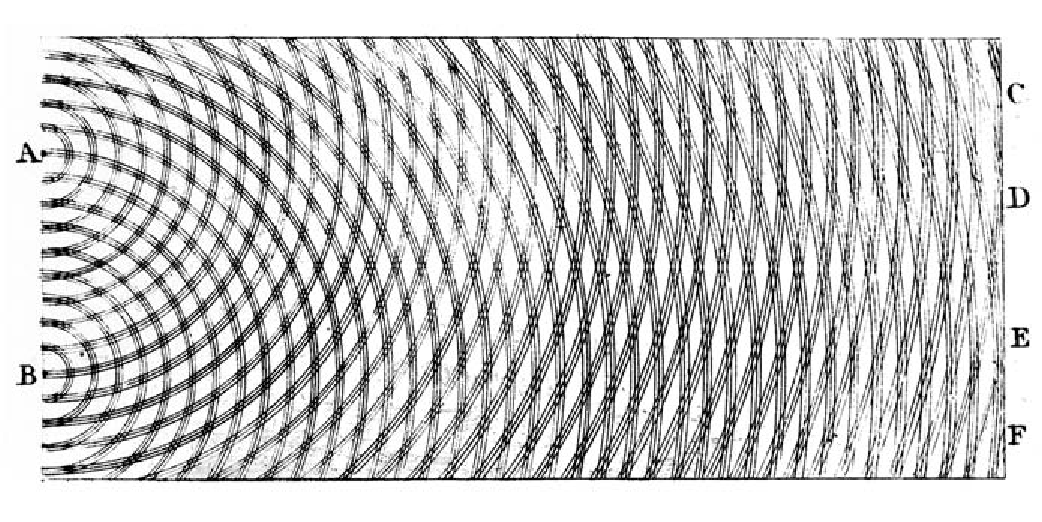
\includegraphics[width=6.75cm]{YoungDiffraction}} 
Un changement de paradigme a lieu � partir de la mise en �vidence des ph�nom�nes d'interf�rences et de diffraction de la lumi�re par Thomas Young et Augustin Fresnel au d�but du $19\ieme$ si�cle. L'illustration ci-contre de Thomas Young~(1803) repr�sente une exp�rience d'interf�rences � double fente. Vers~1850 le mod�le ondulatoire devient la norme. La pr�diction par Maxwell en~1865 du fait que la lumi�re est une onde �lectromagn�tique~\cite{Max65}, suivie de la confirmation exp�rimentale par Hertz en~1888, porte un coup de gr�ce aux th�ories corpusculaires de la lumi�re.

}

\vspace{1ex}
C'est en tentant de mod�liser le \termetech{rayonnement du corps noir} qu'en 1900, Max Planck �met l'hypoth�se que les �changes d'�nergie entre mati�re et rayonnement sont quantifi�s~\cite{Pla01}. Celui-ci pose alors sans le savoir la premi�re pierre de la physique quantique. Presque cinq ans plus tard, Albert Einstein remet en question la nature m�me du rayonnement �lectromagn�tique en stipulant que la quantification de l'�nergie en est une propri�t� fondamentale~\cite{Ein05}. La notion de \termetech{photon} �merge alors, soulignant une dualit� apparemment paradoxale : la lumi�re semble poss�der les propri�t�s � la fois d'une onde et d'un corpuscule.
C'est le d�veloppement de la m�canique quantique, durant les vingt ann�es suivantes, qui va permettre d'interpr�ter cette double nature.


Louis \dB, durant sa th�se de doctorat~\cite{Bro24} en 1923, formule l'hypoth�se selon laquelle 
tout corpuscule mat�riel poss�de des propri�t�s ondulatoires caract�ris�es par une \lo $\lambdaDB$ qui s'exprime :
\[
\lambdaDB = \frac{h}{p}
\virguleformule
\]
o� $h$ est la constante de Planck et $p$ est la quantit� de mouvement de la particule. Cette hypoth�se g�n�ralisait donc aux \emph{particules massive} la dualit� onde-corpuscule.

L'exp�rience de Davisson-Germer, en 1927, apporte la premi�re confirmation exp�rimentale de l'hypoth�se de \dB par l'observation de la diffraction d'�lectrons par un cristal de nickel~\cite{DaG27}. 
La \lo de \dB �tant inversement proportionnelle � la masse et � la vitesse des particules, il est difficile de mettre en �vidence le caract�re ondulatoire des atomes%
%, � moins de les manipuler � tr�s basse temp�rature%
\footnote
{Consid�rons le cas d'un atome l�ger, l'h�lium, pris dans des conditions de temp�rature ambiante. La \lo thermique de \dB est alors:
$
\lambdaDB = \ttfrac{h}{\sqrt{2\,\pi\,m\,\kb\,T}} \approx \SI{0.5}{\angstrom}
,
$
qui est de l'ordre du rayon de l'atome d'h�lium. 
}%
.
%
Il faut attendre les ann�es 1980 pour observer la diffraction d'un jet d'atomes issus d'une source � temp�rature ambiante~\cite{MGA83,KSS88}.
%diff r�seaux~\cite{MGA83}
%diff grating~\cite{KSS88}


\casse


Avec l'apparition des techniques de refroidissement laser~\cite{Phi98,Chu98,Coh98,MeS99} on observe un d�veloppement spectaculaire du domaine de l'\termetech{optique atomique}. Cette discipline, dont la r�f�rence~\cite{Mey01} pr�sente une introduction d�taill�e, consiste � tirer parti des propri�t�s ondulatoires de la mati�re pour des exp�riences de diffraction ou d'interf�rences traditionnellement r�alis�es avec de la lumi�re. 

Dans une exp�rience d'optique atomique, une source d'atomes froids peut �tre consid�r�e comme l'analogue d'une source lumineuse ayant une faible largeur spectrale.
Toutefois, m�me � tr�s faible temp�rature, les sources atomiques ne sont pas parfaitement coh�rentes. 


\section{Quand la mati�re devient une onde coh�rente}

\subsubsection{La lumi�re laser}

La notion de \termetech{laser} a pris naissance avec le concept d'�mission stimul�e introduit par Albert Einstein en 1917~\cite{Ein17}. Mais ce n'est qu'en 1953 qu'est con�u le premier \termetech{maser} (l'analogue du laser pour le domaine des micro-ondes)~\cite{GZT55}. %Au cours des six ann�es suivantes, de nombreux scientifiques tels N. G. Bassov, A. M. Prokhorov, Ch. H. Townes (Prix Nobel 1964) et A. L. Schawlow (Prix Nobel 1981) contribuent � d�velopper le formalisme th�orique pour d�crire le rayonnement maser, puis � adapter leur th�orie aux longueurs d'ondes du rayonnement visible. 
%
En 1960, le physicien am�ricain Th�odore Maiman obtient pour la premi�re fois une �mission laser \emph{puls�e} en utilisant un cristal de rubis comme milieu amplificateur~\cite{MAI60}. Six mois plus tard Ali Javan et ses collaborateurs mettent au point un laser au gaz (h�lium et n�on) dont l'�mission est cette fois-ci \emph{continue}~\cite{JBH61}.

Dans une cavit� laser, un nombre macroscopique de photons occupent tous le m�me mode spatial de propagation et sont coh�rents entre eux (m�me \lo, m�me phase, m�me polarisation). 
Chaque photon fait partie d'une seule et m�me onde macroscopique coh�rente. C'est de cette propri�t� que d�coule la plupart des applications de la lumi�re laser : t�l�communications, m�decine, recherche fondamentale, armement, industrie, etc\ldots

\ifthenelse{\FormatEUE > 0}{}
{\AjouteLigne}

\subsubsection{La \cbe}
En 1924, prolongeant une id�e du physicien indien Satyendranath Bose, Albert Einstein formule une autre pr�diction th�orique : pour un ensemble de particule confin�e sans interaction, en dessous d'une certaine temp�rature critique, un nombre macroscopique d'atomes s'accumulent dans l'�tat d'�nergie minimale%
\footnote{Cette transition ne peut �tre effectu�e que par une certaine classe de particules, appel�es \termetech{bosons}, dont le \termetech{spin} (le moment cin�tique intrins�que) est un multiple entier de $\hbar$.}%
. 
En entrant dans ce r�gime dit de \termetech{d�g�n�rescence quantique}, les atomes occupent tous, de mani�re coh�rente, une m�me fonction d'onde macroscopique, formant 
\inlinefigr{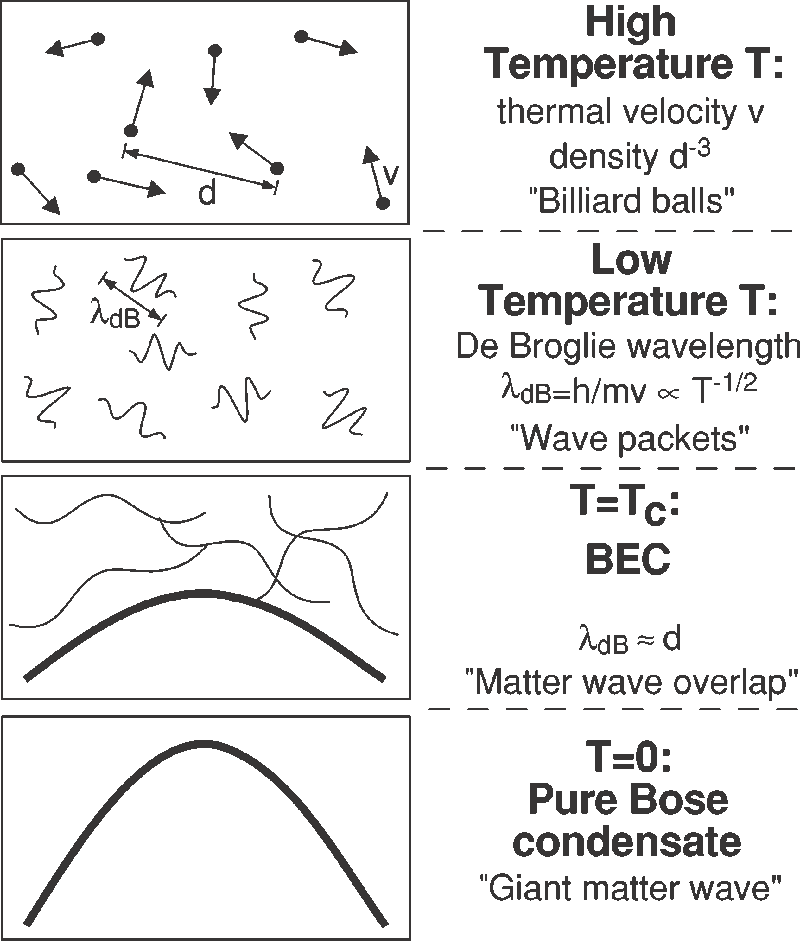
\includegraphics[width=5.5cm]{Ket02}} 
\vspace{-1.5ex}
\noindent
ce qu'on appellera plus tard un \termetech{\bec}. 
Toutefois la \condbe se produit � des temp�ratures si basses qu'il est inimaginable en 1924 que l'on puisse l'atteindre un jour.

Plus de 70 ans plus tard, en combinant les techniques de refroidissement laser avec et du \termetech{\rpef}, Eric Cornell, Carl Wieman et Wolfgang Ketterle produisent en 1995 les premiers \becs~\cite{AEM95,DMA95}. Ils obtiennent pour leurs travaux le Prix Nobel en 2001.

L'illustration ci-contre est issue de la \termetech{conf�rence Nobel} 2001~\cite{Ket02}. Elle sch�matise la \condbe, qui intervient quand la \lo de \dB devient de l'ordre de la distance entre atomes.
\picskip{0}

\casse

Le caract�re coh�rent des \bec a �t� mis en exergue d�s 1997 par l'�quipe du professeur W.~Ketterle~\cite{ATM97}. 
En 2000, le groupe de T.~H�nsch (Prix Nobel 2005) s'est int�ress� � la longueur de coh�rence spatiale d'un \bec. Il observe que la longueur de coh�rence est, pour une g�om�trie \tde, de l'ordre de la taille du \becc%
\footnote{Si pour une g�om�trie \tde la phase de la fonction d'onde est constante sur toute l'extension du \becc, d'autre exp�riences montrent en revanche que, dans une g�om�trie \ude, des fluctuations de phase sont observ�es le long de l'axe longitudinal~\cite{DHR01,RGT03}.}~\cite{BHE00}.

L'analogie entre les photons d'une cavit� laser et les atomes d'un \becc est �vidente. 
La manipulation d'ondes de mati�re coh�rente ouvre alors de nombreuses perspectives : 
\begin{itemize}
	\item en m�trologie, pour mesurer avec une tr�s grande pr�cision des temps, des vitesses de rotation ou des acc�l�rations~\cite{Bor02},
	\item en nano-lithographie, o� l'on peut imaginer graver des structures sub-nanom�trique par interf�rences, 
	\item des mesures interf�rom�triques de grandeurs jusqu'alors inaccessible aux syst�mes optiques, les atomes �tant sensibles � diff�rents champs de force (champ de gravit�, champ magn�tique,\ldots).
\end{itemize}
Cependant, il faut disposer d'un moyen d'extraire, puis de manipuler les atomes d'un \becc, tout en pr�servant leur coh�rence.

\subsubsection{Le \lat}
%Actuellement, plus d'une trentaine de laboratoires de par le monde disposent d'une exp�rience de \condbe. 
L'extraction d'ondes de mati�re coh�rente � partir de ces \beccs a d'ores et d�j� �t� r�alis�e par plusieurs groupes de recherche. Pour ce faire, divers types de coupleur de sortie ont �t� r�alis�s:
\def\spppace{\vspace{1ex}}
\def\hpppace{\hspace{-2em}}
\def\sssize{12cm}

\spppace
\inlinefigr{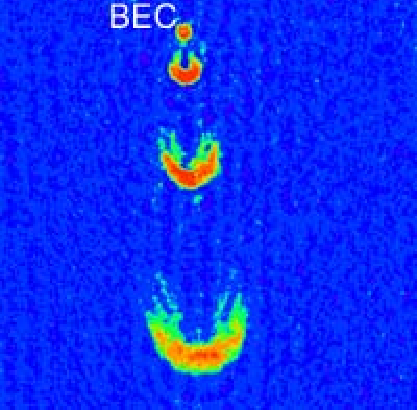
\includegraphics[width=3.5cm]{MAK97a}} 
\hpppace
\begin{minipage}{\sssize}
\begin{ditemize}
	\item en utilisant une impulsion \rf induisant des transitions entre les \snZs, les atomes peuvent passer d'un �tat pi�g� magn�tiquement � un �tat non pi�g�. Un paquet d'ondes de mati�re coh�rente tombe alors sous l'effet de la gravit�~\cite{MAK97}. L'illustration ci-contre est issue de la r�f�rence~\cite{Ket02}.
\end{ditemize}
\end{minipage}

\spppace
\hpppace
\begin{minipage}{\sssize}
\begin{ditemize}
	\item par un sch�ma de couplage utilisant des impulsions laser pour effectuer des transition \termetech{Raman}~\cite{HDK99}. Le paquet d'onde de mati�re est d�coupl� en se voyant communiquer une quantit� de mouvement bien contr�l�e.
\end{ditemize}
\end{minipage}

\spppace
\inlinefigr{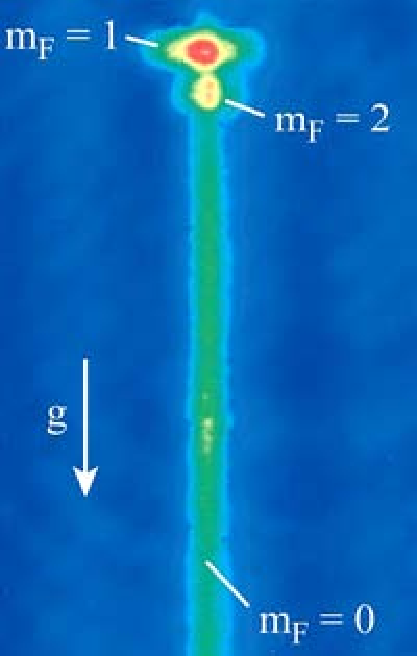
\includegraphics[width=3.5cm]{BHE99a}} 
\hpppace
\begin{minipage}{\sssize}
\begin{ditemize}
	\item il est aussi possible d'obtenir un couplage de sortie continu par application d'une onde \rf. L'extraction \termetech{quasi-continue} peut alors atteindre une dur�e  de \ms{100}~\cite{BHE99} (voir l'illustration ci-contre). Celle-ci n'est limit�e que par le nombre d'atomes initialement pr�sents dans le \becc. Au fur et � mesure que celui-ci se vide, la \rf doit �tre pr�cis�ment ajust�e afin de maintenir un taux de sortie le plus constant possible.
\end{ditemize}
\end{minipage}

\spppace
\hpppace
\begin{minipage}{\sssize}
\begin{ditemize}
	\item le groupe australien du professeur J.~D.~Close a r�cemment mis au point une nouvelle m�thode d'extraction quasi-continue d'atomes � partir d'un \becc pi�g� magn�tiquement gr�ce � une paire de faisceaux Raman ~\cite{RFH06}. 
	%La m�thode d�bouche sur un jet de grande brillance pour une dur�e courte inf�rieure � 10 ms. Elle requiert toutefois un contr�le tr�s pr�cis des champs magn�tiques.
	Ce m�me groupe affirme qu'il n'est d'ailleurs  pas possible d'augmenter arbitrairement le \fat extrait d'un \becc par une m�thode \rf sans impliquer une forte  augmentation des fluctuations d'intensit� du \lat~\cite{RMH05}.
	%En effet, augmenter le taux de couplage de sortie du \becc s'accompagne d'une tr�s forte augmentation des fluctuations d'intensit� du \lat.
\end{ditemize}
\end{minipage}

\picskip{1}~
\casse

%\spppace
%\hpppace
%\begin{minipage}{\sssize}
%\begin{ditemize}
%	\item 
\noindent
	Dans un pi�ge purement optique l'extraction de l'onde de mati�re peut s'obtenir en r�duisant progressivement la puissance des faisceaux lasers en fonction du temps~\cite{CRG03a}. %Les flux qui en r�sultent sont tr�s faibles du fait que le \becc contient initialement seulement \val{E4} atomes. Cette technique a l'avantage de ne pas �tre sensible aux variations des champs magn�tiques. 
%\end{ditemize}
%\end{minipage}



De tels dispositifs sont commun�ment d�sign�s par le terme de \emph{\lat}.
%
%\inlinefigl{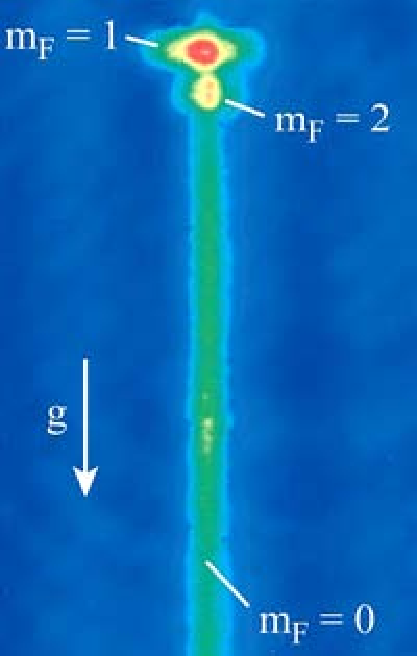
\includegraphics[width=4cm]{BHE99a}} 
%Toujours � l'aide d'une onde \rf, il est possible de mener � bien l'extraction \termetech{quasi-continue} sur une dur�e pouvant atteindre \ms{100}~\cite{BHE99}.
% 
%Le faisceau d'onde de mati�re obtenu par cette m�thode d'extraction continue poss�de un flux de quelques millions d'atomes par seconde sur une dur�e de l'ordre de \ms{100}.
%L'exp�rience pr�sente un tr�s bon accord avec la th�orie d�velopp�e dans l'article, ainsi qu'avec une �tude th�orique approfondie r�alis�e deux ans apr�s dans le groupe d'Alain Aspect~\cite{GBA01}. 
%
%
En toute rigueur, tous les \lats existant � ce jour doivent �tre qualifi�s de \emph{puls�} car l'extraction de l'onde de mati�re m�ne � la d�pl�tion du \becc. Il faut alors en produire un nouveau pour r�p�ter l'op�ration.
%Un autre d�faut majeur de ce type de r�alisation de \lat r�side dans les \fats moyens tr�s faibles qu'elles produisent, de l'ordre de \val{E4} atomes par seconde. 

S'il a fallu � peine six mois, en 1960, pour passer du laser � rubis puls� au laser He-Ne continu, on constate que l'obtention d'une onde de mati�re coh�rente, continue et intense reste toujours un d�fi exp�rimental, treize ans apr�s l'obtention du premier \becc.

\subsubsection{Propri�t�s d'un \lat}
Plusieurs exp�riences ont �t� r�alis�es afin d'�tudier les caract�ristiques des faisceaux d'ondes de mati�re obtenus par extraction coh�rente depuis un \bec. On peut citer des travaux concernant l'�tude des propri�t�s suivantes :
\begin{itemize}
	\item la qualit� du faisceau d'un \lat~\cite{LTR01,RGC06},
	\item sa coh�rence temporelle~\cite{KHE01},
%La coh�rence temporelle mesur�e est � la limite de Fourier, plus la dur�e d'�mission est longue, plus la largeur spectrale est faible (ici 700Hz pour une dur�e d'�mission de \ms{1.5}), ce qui traduit une coh�rence temporelle parfaite. 
	\item ses propri�t�s statistiques (fonction de corr�lation)~\cite{ORK05}.
\end{itemize}
De plus, il a �t� d�montr� qu'un tel faisceau de mati�re coh�rente peut �tre manipul� � la mani�re d'une onde lumineuse. \termetech{R�flexion}, \termetech{focalisation}, \termetech{stockage dans un r�sonateur}; ces termes, habituellement associ�s � des faisceaux optiques, entrent dans le vocabulaire propres aux \lats~\cite{BKG01}.


\ifthenelse{\FormatEUE > 0}{}
{\AjouteLigne}

\section{Vers le \lat continu � grand \fat}
Le caract�re puls� des \lats que nous avons d�crits pr�sente un inconv�nient �vident pour un certain nombre d'applications. De plus ils ne mettent � disposition qu'un tr�s faible flux moyen d'atomes condens�s. C'est en effet cette propri�t� dont il faut tenir compte pour des applications de type nano-lithographie ou certaines mesures de pr�cision. 

%\ApplicationNumerique%
\Remarque
{
Un \bec ($\approx \val{E5}$ atomes) vid� toutes les 5 secondes (temps typique pour reformer un nouveau \becc) donne un flux moyen de quelques \val{2E4} atomes par seconde. Ce qui signifie, pour donner un ordre d'id�e, que le temps n�cessaire pour couvrir un millim�tre carr� d'une monocouche atomique serait d'environ 10 ans \ldots
}
Certaines applications potentielles des \lats n�cessiteraient l'obtention de \fats beaucoup plus �lev�s et, si possible, d'un fonctionnement en continu. 
Pour cela, deux approches semblent possibles :
\begin{itemize}
	\item la premi�re consiste � r�-alimenter le \becc au fur et � mesure de l'extraction de l'onde de mati�re. Un premier pas dans cette direction a �t� fait par l'�quipe de W.~Ketterle en 2002 au \nomofficiel{MIT}~\cite{CSL02}: un \bec pi�g� optiquement est p�riodiquement r�-aliment� par de nouveaux \beccs produits dans une chambre auxiliaire et transport�s � l'aide d'une \termetech{pince optique}.
	\item la seconde possibilit� consiste � produire un \jatg, puis � y adapter la technique d'\evap afin d'atteindre le \rdq. C'est cette m�thode originale, propos�e en 2000 par le groupe \nomofficiel{Atome-Froids} du laboratoire Kastler Brossel (ENS)~\cite{MMD00}, qui fait l'objet de ce m�moire de th�se.
\end{itemize}
%D'apr�s une �tude th�orique effectu�e dans ce m�me groupe, la coh�rence spatiale de ce type de laser serait assez faible selon l'axe de propagation ~\cite{CDM00}
%
%\subsubsection{Une nouvelle approche vers un \lat continu et intense}
%Pour cela nous utilisons une approche originale propos�e en 2000~\cite{MMD00} et qui consiste � refroidir directement un jet atomique guid� magn�tiquement. 
%Le dispositif exp�rimental dont nous disposons repose sur l'injection p�riodique, 5 fois par seconde, de nuages d'atomes froids dans un guide magn�tique de 4,5 m�tres de long. Celui-ci se compose de quatre tubes de cuivre parall�les, refroidis par eau, produisant un champ magn�tique quadrupolaires qui guide les atomes de rubidium pr�par�s dans l'�tat $\EtatFmF{1}{-1}$. Le flux continu est obtenu par le recouvrement spatial des diff�rents paquets atomiques d�s les 50 premiers centim�tres de propagation dans le guide [13]. Les caract�ristiques du faisceau atomique que nous produisons sont les suivantes :
% 	Un flux de \atps{7E9} at / s
% 	Une vitesse moyenne de \cmps{60}
% 	Une temp�rature de \microK{600}
% 	Une densit� dans l'espace des phases d'environ \val{2E-8}
% 	Un taux de collision moyen par atome de \smun{5}
%
%\subsubsection{Etudes th�oriques}
%\cite{CDM00}
%Cet article constitue la premi�re �tude th�orique qui vise � comprendre les propri�t�s de coh�rence d'un jet continu guid� magn�tiquement dans le \rdq. Ces propri�t�s de coh�rence sont �tudi�es par le biais des fonctions de corr�lations longitudinales. Le r�sultat essentiel porte sur le r�le cl� jou� par les interactions. En effet, en l'absence d'interactions la fonction de corr�lation du deuxi�me ordre pr�sente un caract�re poissonien qui traduit des fluctuations importantes du flux de mati�re condens�e. Ce flux est en revanche stabilis� par la pr�sence d'interactions r�pulsives entre les atomes. La fonction de corr�lation du premier ordre a une d�croissance exponentielle avec pour longueur caract�ristique quelques longueurs d'onde de \dB thermique pour la temp�rature du jet. Cette longueur est relativement faible, de l'ordre de quelques microm�tres pour des param�tres exp�rimentaux typiques. Elle ne fait que refl�ter les fluctuations de phase pr�sente dans les g�om�tries � dimensions r�duites~\cite{DHR01,RGT03}.
%
%\subsubsection{Mise en \oe uvre exp�rimentale}
%La premi�re �tape a consist� en l'alimentation en continu d'un guide magn�tique de dimension m�trique~\cite{CRA02}, par opposition � l'�tat de l'art en 2000 o� seuls des paquets d'atomes avaient �t� coupl�s � des guides de dimension centim�trique. R�cemment, le groupe de G. Raithel dans le Michigan~\cite{OMR06} a r�alis� une exp�rience de m�me nature que celle de l'�cole normale sup�rieure. L'objectif est naturellement ensuite de mettre en oeuvre le refroidissement par �vaporation. Le premier pr�requis est d'atteindre le r�gime collisionnel. Cette �tape a �t� franchie en 2004 :
%
%\cite{LVG04}
%
%Dans cet article, un jet continu guid� magn�tiquement est mis hors �quilibre gr�ce � une onde radio-fr�quence. Son retour � l'�quilibre thermodynamique sous l'effet des collisions �lastiques est �tudi� par une m�thode de spectroscopie radio-fr�quence originale.
%
%\cite{LWR05}
%
%Le refroidissement par �vaporation � proprement parler est pr�sent� dans cette derni�re publication. Les auteurs ont cumul� le long du guide magn�tique une dizaine de zones d'�vaporation cons�cutives.
%En ajustant les hauteurs successives de troncature �nerg�tique de la distribution transverse des atomes du jet, ils ont d�montr� un gain d'un ordre de grandeur sur la densit� dans l'espace des phases du jet atomique. Il reste toutefois � gagner 7 ordres de grandeur sur cette derni�re quantit� pour atteindre le \rdq. La limite impos�e au gain en densit� dans l'espace des phases r�sulte du faible nombre de collisions �lastiques (~ 20) que chaque atome subit lors de sa propagation dans le guide magn�tique. Avec un taux de collisions dix fois plus �lev� le \rdq est a priori accessible. Ce groupe �tudie actuellement diff�rentes strat�gies pour atteindre ce dernier objectif.
%







\casse


\section{Pr�sentation des travaux}% : une nouvelle approche vers un \lat continu et intense}

Le travail r�alis� au cours de ma th�se peut se d�composer en trois parties, chacune contenant deux chapitres.
Les diff�rents th�mes de recherche qui seront pr�sent�s dans ce m�moire de th�se ont tous donn� lieu � la r�daction d'un article scientifique~\cite{LWR05,LRW06,RWC06,RLC06,CKR08,RLW07,CJK08,ReG08}. Les r�f�rences et r�sum�s de ces articles sont r�unis dans l'annexe~\nref{annexe:Articles} (\vpageref{annexe:Articles}).

\ifthenelse{\FormatEUE > 0}{}
{\AjouteLigne}

\subsubsection{Premi�re partie: \TitrePartieUn}
%Cette partie traitera de la formation et de l'�vaporation d'un \jatgm:
\begin{ditemize}
%
	\item le chapitre \ref{chap:JetAtomique} introduit les concepts qui vont servir de supports aux diff�rentes analyses li�es au guidage magn�tique. Nous y pr�senterons notamment le \setup tel qu'il existait � mon arriv�e dans l'�quipe de \dgo. L'�tude du \jatgm avait alors d�j� montr� que le \tcolel �tait suffisant pour pouvoir mettre en \oe uvre le \rpef. \`A l'issue de ma premi�re ann�e de th�se, nous avons ainsi pu mettre en �vidence un gain d'un ordre de grandeur sur la densit� dans l'espace des phases du jet~\cite{LWR05}.
%
	\item le chapitre \ref{chap:Ceramique} pr�sente une technique efficace permettant de mener � bien l'\evap d'un \jatmg. Nous avons adapt� le principe d'�limination d'atomes �nerg�tiques au contact d'une surface mat�rielle~\cite{HMO03} � notre \setup. 
%
\end{ditemize}
Dans la premi�re partie nous soulignerons le fait que l'�vaporation d'un \jat est une t�che fondamentalement plus ardue que celle mise en \oe uvre habituellement sur un nuage pi�g�. Afin de pouvoir atteindre le \rdq, nous conclurons sur la n�cessit� de d�velopper de nouveaux outils permettant d'augmenter le nombre de \colels au sein du jet. 


\subsubsection{Deuxi�me partie: \TitrePartieDeux}
%Cette partie traitera de la manipulation et du refroidissement de \pats dilu�s, lors de leur propagation dans le \gm:
%Le param�tre physique qui nous limite est le nombre moyen $\Ncol$ de collisions subies par un atome au cours de sa propagation. Une estimation montre que si nous pouvions disposer d'un nombre dix fois plus �lev� de collisions (soit $\Ncol\approx200$), le \rdq serait alors accessible.
\begin{ditemize}
%
	\item le chapitre \ref{chap:MiroirMobile} d�crit la mise en \oe uvre d'une technique de ralentissement de \pats guid�s par r�flexion sur un \mimamo. Nous y d�montrons l'efficacit� de cette m�thode ainsi que l'int�r�t qu'elle pr�sente dans le contexte de la production d'un \jatuf continu et dense~\cite{RLC06}. Nous serons d'ailleurs amen�s � comparer l'action du \mimo sur les \ps avec celle d'un \termetech{d�mon de Maxwell}~\cite{ReG08}.
%
	\item le chapitre \ref{chap:Convoyeur} pr�sente une technique originale permettant de capturer les \pats guid�s dans un \tpm \tds fait d'aimants permanents~\cite{LRW06}. Nous expliciterons, avec l'appui de simulations num�riques, les m�canismes physiques � l'\oe uvre dans ce probl�me de transport. 
Nous y pr�senterons enfin les r�sultats d�montrant le transport ainsi que le refroidissement des paquets pi�g�s dans le \tpm.

%
\end{ditemize}
 
%\pagebreak
 
\subsubsection{Troisi�me partie: \TitrePartieTrois}
%Dans cette derni�re partie, nous �tudierons la possibilit� de produire, manipuler et �tudier des \nats denses:
\begin{ditemize}
%
	\item le chapitre \ref{chap:PiegeDipolaire} pr�sente une m�thode de production de \pats tr�s denses gr�ce � un pi�ge optique � force dipolaire. Nous y traiterons aussi de la mise en mouvement de ces \ns. Un mod�le analytique simple nous servira de support pour pr�senter les r�sultats exp�rimentaux li�s � l'optimisation du transport~\cite{CKR08}.
%
	\item le chapitre \ref{chap:Imagerie} d�crit un nouveau protocole d'imagerie que nous avons d�velopp� lors de ma deuxi�me ann�e de th�se. En effet, les deux techniques pr�dominantes pour faire l'image d'ensembles atomiques dilu�s, � savoir l'\termetech{imagerie par absorption � faible intensit�} et l'\termetech{imagerie par fluorescence}, s'av�rent peu fiables lorsqu'il s'agit de traiter des \ns dont la \pro exc�de \val{4}-\val{5}.
Notre protocole permet de r�soudre les structures de \nats denses et donne acc�s � des mesures quantitatives et pr�cises~\cite{RLW07}. 
%
\end{ditemize}
 


%\subsubsection{Condensation de Bose~\cite{CJK08}}
%Pr�cisons enfin qu'en utilisant une configuration de faisceaux crois�s  avec notre laser de puissance, nous avons r�cemment r�alis� un \bec. Celui-ci contient typiquement \val{E5} atomes et est r�aliser en 6 secondes. Nous pouvons contr�ler pr�cis�ment l'�tat interne des atomes qui le compose en utilisant une m�thode de distillation de spin par application de gradients de champs magn�tiques au cours de l'�vaporation. Cette technique de contr�le des �tats internes a �t� mise � profit pour extraire du \becc un \lat guid� optiquement~\cite{CJK08}.



\DontNumberThisInToc
\part{\TitrePartieUn}
%\NumberThisInToc
\chapter*{Introduction : une th�se dans les atomes froids}

\minitoc

Ultracold and slow beams have a huge potential in metrology, matter wave interferometry and nanolithography~\cite{Ber97}.


Un tel faisceau est d'importance cruciale  pour r�aliser un laser � atome continu g�n�rer par un processus d'�vaporation forc�e appliqu�e � un jet continu guid� magn�tiquement, comme propos� dans~\cite{MMD00} et �tudi� exp�rimentalement dans~\cite{LWR05}

\section{La physique des atomes-froids}

L'�tude des ph�nom�ne physiques fondamentaux � l'echelle microscopqiue. 

\subsection{Les diff�rentes �tape du refroidissement d'un ensemble atomique}\label{sec:EtapesRefroidissement}

Temp�rature ambiante : \SI{300}{\kelvin}.

\subsection{Laser cooling}\label{sec:Laser cooling}
PAGE 2 Cornelussen

\subsection{Bose-Einstein condensation}\label{sec:BoseEinsteinCondensation}
PAGE 4 Cornelussen


	\subsection{Potentiel magn�tique de pi�geage}\label{sec:PiegeageMagnetique}

Nous allons rappeler ici le principe de la manipulation et de pi�geage magn�tique d'atomes neutres paramagn�tiques\footnote{C'est � dire, poss�dant un moment magn�tique permanent.}. 
Cette technique de pi�geage non dissipatif qui a �t� mise en \oe uvre pour la premi�re fois en 1985~\cite{MPP85} � conduit, dix en plus tard � la possibilit� de refroidir un \nat jusqu'au seuil de \condbe~\cite{AEM95,DMA95,CoW02,Ket02}.

	 \subsubsection{L'effet Zeeman sur le niveau fondamental du \Rb}

L'effet Zeeman sur les \snhfs du fondamental permet la manipulation des atomes de \Rb gr�ce � des gradients de \chm. La formule de Breit-Rabi\cite{BrR31} donne l'�nergie d'un atome plong� dans un \chm d'intensit� $\modB$ en fonction de son �tat interne (cette formule est ici appliqu�e au cas d'un atome de \Rb dans son �tat fondamental \OrbitalS):
\begin{align}
	E_{F,\mF}(\modB) = &
	(-1)^F \, \frac{\hbar\,\omegaHF}{2}
	\, \sqrt{1+ {\mF} \, x + x^2} + \const ,	\label{eq:BreitRabi} \\ 
	\mbox{avec  } x = & \frac{(g_I + g_S) \, \muB}{\hbar\,\omegaHF}\,\modB , \nonumber
\end{align}
et o� $\hbar\,\omegaHF$ d�signe la s�paration en �nergie des deux \snhfs en l'absence  de \chm, $g_I$ et $g_S$ sont les facteurs gyromagn�tiques du noyaux et de l'�lectron respectivement (ces valeurs sont rappel�es dans le tableau \vref{tab:ChiffresRb}). $\mF$ est le nombre quantique magn�tique de l'�lectron. l'�nergie $E_{F,\mF}(\modB)$ est donn�e � une constante pr�s, qui rend compte de l'�nergie des \snx en l'absence de \chm.

	 \subsubsection{Pi�geage magn�tique}
Le pi�geage magn�to-statique de particules paramagn�tiques repose sur l'utilisation d'un gradient de potentiel magn�tique. En pratique, la s�paration des \snx due � l'effet Zeeman est faible devant l'�cart �nerg�tique entre les deux �tats \hfs du fondamental\footnote{Les \chm utilis�s dans la pratique sont en effet de quelques centaines de Gauss au maximum. Pour acc�der � des valeurs de $x$ proches de 1 il faut appliquer des champs de quelques $\val{E4}$ Gauss} ($x \ll 1$). L'expression~\nref{eq:BreitRabi} peut donc �tre d�velopp�e au premier ordre en $\modB$:
\begin{equation}
	E_{F,\mF}(\modB) \approx \mF\,g_F\,\muB\,\modB ,
	\label{eq:EZeeman}
\end{equation}
o� nous d�finissons le facteur de Land�\footnote{$\Module{g_F} = \tfrac{1}{4}\,(g_I + g_S)$ n'est pas tout � fait �gal $\tfrac{1}{2}$, mais sa valeur en est proche � moins de $\val{E-3}$ pr�s. On utilise g�n�ralement cette valeur, de la m�me mani�re qu'on utilise la valeur  $2$ pour le facteur gyromagn�tique de l'�lectron.} $g_F \equiv (-1)^F\,\tfrac{1}{4}\,(g_I + g_S) \approx (-1)^F\,\tfrac{1}{2}$. Dans toute la suite, nous aurons pour convention de noter \[ \mu \equiv \mF\,g_F\,\muB, \] le moment magn�tique de l'atome dans l'�tat $\Etat{F,\mF}$ consid�r�. 
Un atome de \Rb plong� dans un \chm inhomog�ne $\vectBr$ sera soumis au potentiel $U(\Vecteur{r}) = \mu\,\modBr$. La force qui d�rive de ce potentiel tend � pousser les atomes vers les zones de champs faibles s'ils sont pr�par�s dans l'un des �tats
\footnote{Gardons n�anmoins � l'esprit que l'expression~\nref{eq:EZeeman} n'est qu'un d�veloppement limit� � l'ordre 1 en \chm. En utilisant la formule~\nref{eq:BreitRabi}, on constate que l'�tat $\EtatFmF{2}{0}$ est aussi pouss� vers les zones de champ faible. C'est l'effet Zeeman quadratique. En pratique cependant, cet effet est suffisamment faible pour ne pas �tre exploitable.}  
\[ \EtatFmF{1}{-1} \mbox{, } \EtatFmF{2}{1} \mbox{, ou } \EtatFmF{2}{2} , \] 
et vers les zones de champs forts s'ils sont pr�par�s dans 
\[ \EtatFmF{1}{1} \mbox{, } \EtatFmF{2}{-1} \mbox{, ou }  \EtatFmF{2}{-2} . \] 
Il est donc logiquement possible de pi�ger magn�tiquement des atomes gr�ce � un extr�mum local de la norme du champ magn�tique. Les �quations de Maxwell interdisent cependant l'existence d'un maximum local de \chm dans le vide.
\Remarque{
\subsubsection{Impossibilit� d'avoir un maximum de \chm dans le vide} 
Celle-ci vient du fait que le laplacien du module du champ ne peut �tre n�gatif dans le vide. 

\noindent Pour mieux comprendre, consid�rons plut�t le module carr� du champ qui varie bien s�r dans le m�me sens que le module, mais qui a l'avantage de s'exprimer gr�ce � un produit scalaire. Apr�s quelques lignes d'alg�bres �l�mentaire, on montre que le laplacien de cette grandeur: 
\[ \Delta \left( \modB^2 \right)
  \equiv \Delta\left( {B_x}^2 + {B_y}^2 + {B_z}^2 \right) , \] 
ne peut �tre n�gatif (c'est une cons�quence directe du fait que, dans le vide, $\Delta( \vectB )$ est nul). Or, un laplacien n�gatif est une condition n�cessaire (bien que non suffisante) pour avoir un maximum de la norme au carr�, et donc de la norme du \chm.}
Si l'on d�sire pi�ger des atomes gr�ce � un champ magn�to-statique, il faudra donc les pr�parer dans un �tat \sotosay{attir� par les champs faibles}. C'est de ces �tats dont il sera question dans toute la suite, et nous ne consid�rerons donc plus les �tats non-pi�geables. De plus, pour des raisons pratiques li�es � la d�tections des atomes dans le guide (voir \autoref{sec:MesureJat}), la totalit� des exp�riences dont il sera question ici fait intervenir des atomes pr�par�s dans l'�tat \EtatSFmF{1}{-1}.

\Remarque{
\subsubsection{Perte Majorana}\label{Rq:Majorana}
Pi�ger les atomes en utilisant un \chm inhomog�ne suppose une chose en particulier: 
\begin{itemize}
	\item le moment magn�tique de l'atome doit rester en permanence align� avec le vecteur \chm local.
\end{itemize}
Or, s'il est possible de r�aliser un minimum de la norme du champ, celui-ci ne peut alors pas avoir une direction constante (l'�quation de Maxwell $\Divergence{\vectBr} = 0$ l'interdit). 

\noindent Ainsi, un atome, dans son mouvement autour du minimum de potentiel, va en permanence \sotosay{voir} le vecteur \chm changer de direction. Ceci implique que les �tats propres de l'hamiltonien varient le long de la trajectoire de l'atome, et il existe une probabilit� non-nulle pour que ce dernier change d'�tat de spin. Ce m�canisme de transition d'un �tat pi�g�, � un �tat non-pi�g� porte le nom de pertes Majorana\cite{SuB97}.
		
Afin que la probabilit� de d'effectuer ce type de transition  reste faible, il faut que les variations du \chm $\vectBr$ \sotosay{vu par l'atome} soient lentes devant l'�chelle de temps d�finie par la pulsation $\omegaL$ de la pr�cession de Larmor:
\begin{equation}
	{\left. \frac{\mathrm{d}\,\vectB}{\mathrm{d} t} \right.} \ll \omegaL \equiv \gamma\,\modB
	\label{eq:PasMajorana}
\end{equation}  
o� $\gamma$ est le rapport gyromagn�tique de l'�lectron et vaut $\gamma \approx \SI{1,4}{\mega\hertz\per G}$. Pour se mettre dans de bonnes conditions, il faut �viter d'avoir des zones dans lesquelles le \chm est trop faible, et ce pour 2 raisons: \begin{itemize}
	\item Un faible \chm correspond � une faible fr�quence de Larmor, ce qui ne va pas dans le sens de l'�quation \vref{eq:PasMajorana}.
	\item Au voisinage d'un minimum local de \chm, les variations de direction du vecteur champ sont d'autant plus violentes que la valeur du champ est faible.
\end{itemize}
}

Top Trap~\cite{PAE95}

Magnetic trapping of neutral particles: Classical and quantum-mechanical study of a Ioffe-Pritchard type trap~\cite{GST00}
	
	\subsection{Le \rpef}\label{sec:RefEvap}


\section{Situation du sujet}
\subsection{La condensation de Bose-Einstein}\label{sec:condensation}
\subsubsection{La \ddedpup}
\subsection{Manipulation d'ondes de mati�re coh�rentes}
\subsection{Le \lat}
\subsection{Ce qu'il reste � faire}

\section{But principal de l'exp�rience : le \emph{laser � atome continu}}
\subsection{R�alisation d'un \jatuf et intense}
d�finir temp�rature transverse quelque part
\subsection{�vaporation forc�e}\label{sec:EvapForcee}
\subsection{Vers une source coh�rente et intense d'onde de mati�re}

\section{Les chiffres � conna�tre}\label{sec:Chiffres}

azeaze

\begin{tabular}{|l|c|c|}
   \hline
   d�finition & 
   symbole & 
   valeur \\
   \hline
   Vitesse de la lumi�re dans le vide & 
   $c$ & 
   $\mps{299792458}$ (valeur exacte)\\
   \hline
   Perm�abilit� du vide & 
   $\mu_0$ & 
   $4\,\pi\,\SI{E-7}{\newton\per\ampere\squared}$ (valeur exacte)\\
   \hline
   Permitivit� du vide & 
   $\epsilon_0$ & 
   $\left(\mu_0\,c^2\right)^{-1} = \SI{8,8542E{-12}}{\farad\per\meter}$\\
   \hline
    & & \\
   \hline
    & & \\
   \hline
   Charge �lectrique �l�mentaire & $e$ & \SI{1,602E{-19}}{\coulomb} \\
   \hline
   Magn�ton de Bohr & $\muB$ & \SI{9,274E{-24}}{\joule\per\tesla} \\
   %\hline
   Constante de Plank & $h$ & \SI{6,626E{-34}}{\joule\second} \\
   \hline
   Constante de Plank & $\hbar$ & \SI{1,055E{-34}}{\joule\second} \\
   \hline
   \label{tab:Chiffres}
\end{tabular}

\begin{tabular}{|l|c|c|}
   \hline
   d�finition & symbole & valeur \\
   \hline
   Num�ro atomique & $Z$ & $ 37 $\\
   \hline
   Nombre de nucl�ons & $Z+N$ & $ 87 $\\
   \hline
   Masse atomique & $ \mRb $ & $\SI{1,44E-25}{\kilogram}$\\
   \hline
   Spin nucl�aire & $ I $ & $ \tfrac{3}{2} $\\
   \hline
   Longueur de diffusion dans l'onde $s$ & $ a $ & $ \SI{5,3E{-9}}{\meter} $ \\
   \hline
   Section efficace de collision dans l'onde $s$ & $ \sigma $ & $ \SI{7,1E{-16}}{\square\meter} $ \\
   \hline
   Dur�e de vide d'un niveau excit� \OrbitalP & $ \tSpont $ & $ \ns{26,2} $ \\
   \hline
   Taux d'�mission spontan�e depuis \OrbitalP & $ \pulsSpont $ & $ \SI{38,1E6}{\reciprocal\second} $ \\
   \hline
   sigma plus et isotrope ! ! ! & $ \Isat_\TransCycle $ & $  $ \\
   \hline
   \label{tab:ChiffresRb}
\end{tabular}

\begin{tabular}{|l|c|c|}
   \hline
   Seuil typique & Temp�rature \Rb & Dispersion de vitesse \\
   \hline
    & $  $ & $  $ \\
   \hline
   Temp�rature Doppler & \microK{146} & \mps{0,118} \\
   \hline
    & $  $ & $  $ \\
   \hline
   Temp�rature de recule & \microK{0,362} & \mmps{5,88} \\
   \hline
    & $  $ & $  $ \\
   \hline
   \label{tab:ChiffresRbFroid}
\end{tabular}


\subsection{L'atome de Rubidium 87}
	\subsubsection{Carte d'identit�}
	\inlinefig{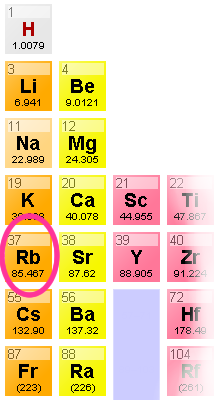
\includegraphics[height = 5cm]{P1/Rb87}}%http://www.dayah.com/periodic/
Le \rb est un m�tal mou et argent� qui devient liquide vers \SI{40}{\degreecelsius}. Il est d�couvert en 1961 par Robert Wilhelm Bunsen et par Gustav Kirchhoff. On le trouve sous forme de trace dans certain minerais. Avec un noyau comptant $Z=37$ protons, cet �l�ment se situ� sur la 5�me ligne de la premi�re colonne de la classification p�riodique des �l�ments. C'est un m�tal alcalin qui r�agit de mani�re explosive au contact de l'eau. 

Parmi les 24 isotopes du \rb, seuls deux sont pr�sents � l'�tat naturel le \RbCinq (\val{72,2}\%) et le \Rb (\val{27,8}\%), ce dernier est tr�s l�g�rement radioactif (avec une demi-vie de 50 millards d'ann�es). Nous ne parlerons � partir de maintenant que du \Rb.

	\subsubsection{Propri�t�es quantiques}
Le cort�ge d'�lectrons du \rb sature compl�tement les 4 premi�res couches electroniques. Un seul �lectron p�riph�rique occupe la cinqui�me couche, ce qui rend mod�lisation des niveaux �nergetiques tr�s simple.

La structure atomique du \rb, avec 37 �lectrons, 37 protons, et 48 ou 50 neutrons (pour le \Rb ou le \RbCinq respectivement), en fait un boson. 

\bfig
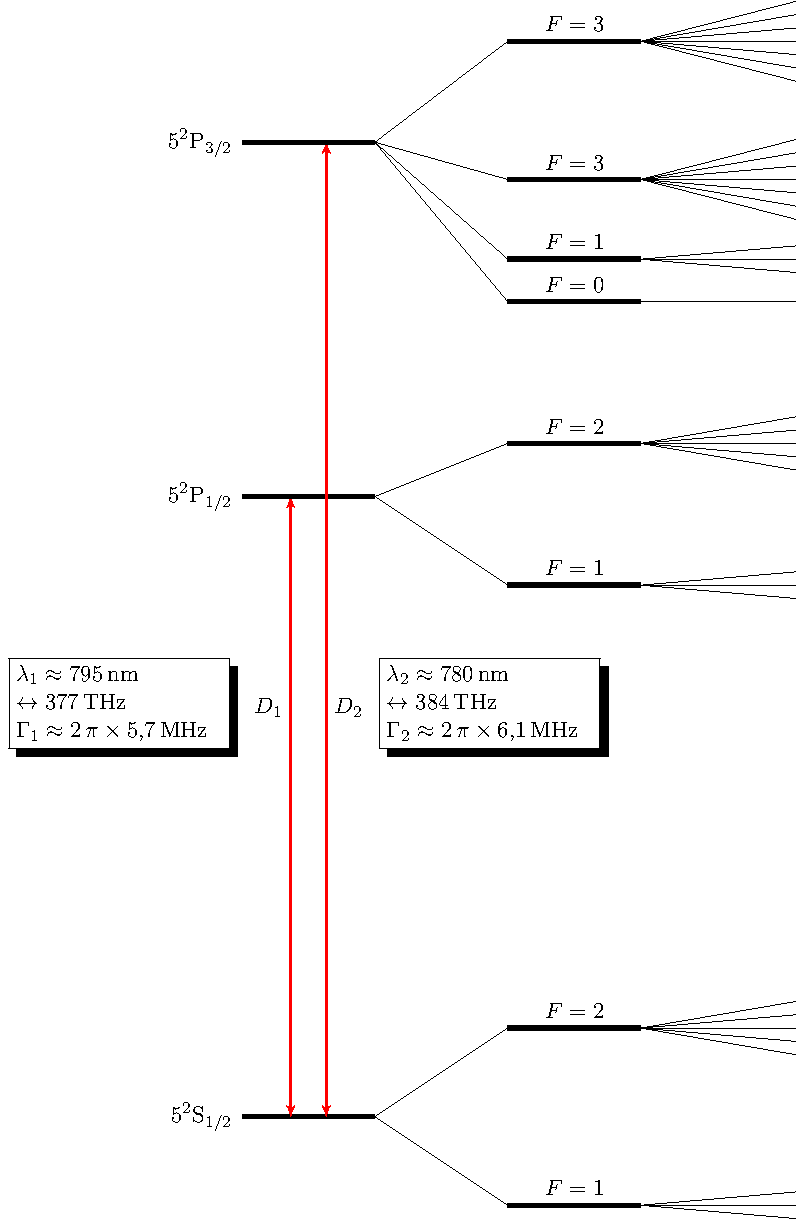
\includegraphics{P1/RbNiveaux}
\CaptionFig{Structure hyperfine des orbitales $\OrbitalS$, $\OrbitalPJun$ et $\OrbitalPJdeux$ du \Rb.}
\label{fig:RbNiveaux}
\efig


	\subsubsection{Pourquoi le \Rb}
Beaucoup d'\exatfs utilisent le \rb. Celui-ci pr�sente plusieurs avantage technique pour l'exp�rimentateur qui souhaite mener � bien le refroidissement d'ensemble atomique. En voici une liste:
\begin{itemize}
	\item Les raies optiques d'excitation se trouve dans le proche infra-rouge, dans un domaine facilement accessible avec des laser � semi-conducteur (diode-laser).
	\item Une pression de vapeur saturante �lev�e qui permet une manipulation facilit� en utilisation sous \uv.
	\item 
\end{itemize}

Le \Rb est tr�s utilis� dans les exp�riences d'atomes froids.

Rb85 diffusion n�gatif -> attractif, colapse

Rb87 repulsif



 Le tableau ci-dessous r�sume quelques une de ses caract�ristiques:

		\begin{tabular}{|r||c|c|}
		\hline
		Num�ro atomique & Z & 37\\
		\hline
		Nombre de nucl�ons & Z+N & 87\\
		\hline
		Masse & m & \SI{1,44E{-25}}{\kilogram}\\
		\hline
		\end{tabular}
		
		
		
\subsection{Mesurer la temp�rature d'un nuages atomiques ultra-froids}

\subsection{La table d'optique}

\subsection{L'ultravide}

\subsection{L'outil informatique}

\Remarque{Un �largissement inhomog�ne, de mani�re plus g�n�ral, est d�fini par le fait que chaque atome poss�de une fr�quence de r�sonance diff�rente. L'exemple typique d'�largissement inhomog�ne est l'�largissement par effet Doppler (la fr�quence de r�sonance d�pend de la vitesse de l'atome consid�r�). Ceci s'oppose � l'�largissement homog�ne, pour lequel tous les atomes se comportent de la m�me mani�re. Un exemple typique est l'�largissement d� aux collisions inter-atomiques dans les gaz sous haute pression.} 


\chapter{\TitreChapitreUn}%
\label{chap:JetAtomique}

\bfigh
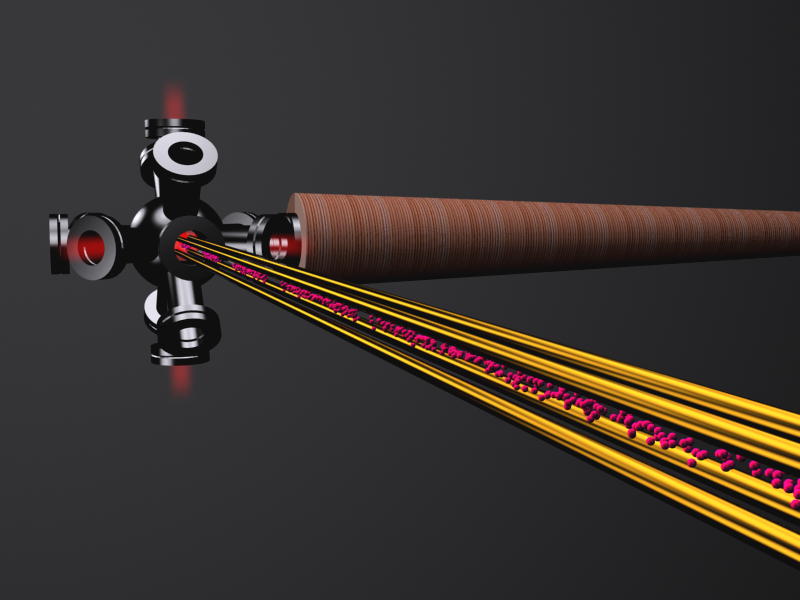
\includegraphics[width=\FigWidth]{P1/ChapitreJetAtomique}
\SansCaption
\efigh

\pagebreak

\minitoc
\vspace{0.5cm}

%Les deux premi�res parties de ce manuscrit auront pour objet l'�tude du comportement d'ensembles atomiques se propageant dans un \gm. 
Ce chapitre a pour but d'introduire les concepts qui vont servir de support aux diff�rentes analyses li�es au guidage magn�tique d'atomes. Nous y pr�senterons notamment le \setup tel qu'il �tait � mon arriv�e dans l'�quipe de \dgo. L'�tude du \jatgm avait alors d�j� montr� que le \tcolel �tait suffisant pour pouvoir mettre en \oe uvre le \rpef. 
La plupart des th�mes abord�s dans ce chapitre font l'objet d'une pr�sentation d�taill�e dans la th�se de Thierry Lahaye~\cite{TTL} � laquelle il sera donc r�guli�rement fait r�f�rence.
Les concepts que j'ai eus � manipuler et les r�sultats importants obtenus lors de ma premi�re ann�e de th�se seront rappel�s.

Dans ce chapitre, nous allons d�crire la configuration magn�tique choisie pour r�aliser le guidage d'atomes sur notre \setup. Le principe d'obtention d'un jet \uf et intense d'atomes de \Rb sera ensuite d�taill�. Nous aborderons la description du processus d'�vaporation forc�e, apr�s avoir �tudi� les diff�rentes mani�res de caract�riser le jet.

\section{Pi�geage dans un \gm \qp}\label{sec:PiegeageMagnetiqueGuide}

L'�l�ment le plus caract�ristique du \setup, qui a servi de support � ma premi�re ann�e de th�se, est un \gm d'une longueur $\Lguide=\m{4.5}$. 
Le guidage d'atomes neutres le long de structures filiformes parcourues par des courants est un domaine qui s'est fortement d�velopp� depuis une dizaine d'ann�es~\cite{Sch95,KHR00,DLL00,TeR01,SBC01}. 
Cette section vise � d�crire la configuration utilis�e pour mener � bien le guidage d'un \jatuf et intense.

\casse

	\subsection{Configuration \qp de \chm}\label{sec:ConfigMagnetiqueGuide}
La configuration qui � �t� choisie sur notre \setup pour guider magn�tiquement les atomes de \Rb est celle d'un \chm \qpdd~\cite{HiE00} cr�� par quatre tubes de cuivre parall�les parcourus par des courants deux � deux oppos�s (voir la figure~\nref{fig:TubesQuadrupole}).
%
\bfigh
\subfloat[Photo du \gm]{\label{TubesQuadrupole_0}
%\begin{overpic}
\includegraphics%
[height=6cm]{P1/TubesQuadrupole_0}
%\end{overpic}	
}\\
\subfloat[Lignes de champ]{\label{TubesQuadrupole_a}
%\begin{overpic}
\includegraphics%
[height=6cm]{P1/TubesQuadrupole_a}
%\end{overpic}	
}
\subfloat[Lignes �quipotentielles]{\label{TubesQuadrupole_b}
%\begin{overpic}
\includegraphics%
[height=6cm]{P1/TubesQuadrupole_b}
%\end{overpic}	
}
\CaptionFig{Positionnement des tubes de cuivre et orientation des courants d'un syst�me produisant un \chm \qpdd. \\
(a): Photographie repr�sentant le \gm. Il est plac� dans un tube de verre � l'int�rieur duquel r�gne un vide pouss�. On distingue l'une des pi�ces en c�ramique qui permet de maintenir les tubes de cuivre en position.\\
(b): Coupe dans le plan ($x,y$) perpendiculaire � l'axe du guide repr�sentant le positionnement des tubes ainsi que quelques lignes de \chm. L'espacement entre deux tubes adjacents est not� $\espTubes$, et le courant qui les traverse est not� $I$. \\
(c): Sch�ma � l'�chelle $3$ sur lequel sont repr�sent�es des �quipotentielles (\cad des lignes suivant lesquelles le module du \chm est constant). Sur tout l'axe $z$, normal au plan de la figure, le module du champ s'annule. %Les lignes de champ repr�sent�es sur la figure (a) montrent bien une forte variation de la direction du vecteur champ autour du minimum.
}
\label{fig:TubesQuadrupole}
\efigh


L'expression du \chm cr�� par un tel syst�me au voisinage de l'axe $z$ est:
\begin{equation}
	\vectBxyz = \vVecteur{-\gradB\,x}{\gradB\,y}{0} \mbox{\qquad avec \qquad} \gradB \equiv \frac{4\,\mu_0}{\pi\,\espTubes^2}\,I ,
	\label{eq:BQuadr}
\end{equation}
o� $\gradB$ 
%
\nome{\gradB}{Gradient transverse de \chm au voisinage de l'axe $z$}
%
 est le gradient transverse de \chm au voisinage de l'axe $z$ et $\espTubes$ est l'espacement entre les axes de deux tubes adjacents
%
\nome{\espTubes}{Espacement entre les axes de tubes adjacents du \gm}%
. 
Cette expression est le r�sultat d'un d�veloppement limit� � l'ordre~1 en $x$ et $y$ de la somme des contributions des \chms produits par les 4 tubes%
\footnote{L'utilisation de cette expression approch�e conduit � faire une erreur inf�rieure � $\val{0.5}\%$ sur le module du \chm pour une distance �  l'axe typique de $\ttfrac{\espTubes}{4}$. C'est donc une tr�s bonne aprroximation.}%
.

\ApplicationNumeriqueTitre{\gtchm}{
Calculons le gradient $\gradB$ sachant que:
\begin{itemize}
	\item le courant $I$ dans les tubes de cuivre du \gm peut monter jusqu'� une valeur de \SI{400}{\ampere},
	\item l'espacement entre deux tubes adjacents est $\espTubes=\mm{8}$.
\end{itemize}
En utilisant le courant maximal, on obtient un \gtchm :
\[
 \gradB = \SI{1}{\kilo G \per\centi\meter}
 \pointformule
\]
Pour comparaison, cette valeur est pr�s de \val{10} fois sup�rieure � celles obtenues typiquement dans des pi�ges de \IP pour les exp�riences de \condbe. 
}
\Remarque{
La puissance dissip�e par effet joule dans le guide peut atteindre quelques kilowatts. C'est pourquoi nous utilisons un syst�me de refroidissement � eau. Celle-ci circule dans les tubes. On se reportera � la th�se de T.~Lahaye~\cite{TTL} pour avoir des d�tails sur les contraintes techniques li�es � la mise en \oe uvre de ce \gm dans un environnement \uv.
}

\subsubsection{Pi�geage magn�to-statique}
Dans les conditions de nos exp�riences, le potentiel magn�tique d'un atome de \Rb immerg� dans un champ $\Vecteur{B}$ est~\cite{MPP85}:
\begin{equation}
	U \approx \mF\,g_F\,\muB\,\modB ,
	\label{eq:EZeeman}
\end{equation}
o� $\muB$ est le \termetech{magn�ton de Bohr}, $g_F \approx \tfrac{(-1)^F}{2}$
est le facteur de Land� de l'�tat hyperfin de moment angulaire $F$ %
%\footnote{$\Module{g_F} = \tfrac{1}{4}\,(g_I + g_S)$ n'est pas tout � fait �gal $\tfrac{1}{2}$, mais sa valeur en est proche � moins de $\val{E-3}$ pr�s. On utilise g�n�ralement cette valeur, de la m�me mani�re qu'on utilise la valeur  $2$ pour le facteur gyromagn�tique de l'�lectron.}%
 et $\mF$ est le nombre quantique magn�tique de l'atome.
Dans toute la suite, nous aurons pour convention de noter :%
\nome{\mu}{Moment magn�tique de l'atome}%
\[ 
\mu \equiv \mF\,g_F\,\muB
\virguleformule
\]
le moment magn�tique de l'atome dans l'�tat $\Etat{F,\mF}$ consid�r�. Pour un atome de \Rb dans l'�tat $\EtatSFmF{1}{-1}$, on a $\mu\approx\SI{4.64}{\joule\per\tesla}$.
%La force qui d�rive du potentiel~\nref{eq:EZeeman} 

\casse

\subsubsection{Confinement lin�aire}
\inlinefig
{
\begin{tikzpicture}
\tkzInit[xmin=-3,xmax=3,ymin=-0,ymax=4]
\tkzX[ orig, noticks,label=$r$]%,poslabel=-0.5cm]
\tkzY[label=$\Ulin$, noticks]
\tkzFct[samples = 200,lw = 1pt,color = red](-4..4){(2*x*x+0)**(0.5)}
%\tkzFct[samples = 200,lw = 1pt,color = gray, style=dashed](-4..4){(2*x*x+0)**(0.5)}
\end{tikzpicture}
}
Pour la configuration d�crite ci-dessus, le potentiel auquel sont soumis les atomes dans le \gm est:
\begin{align}
	\Ulin(x,y,z) 	&= \mu\,\sqrt{\Bx^2+\By^2+\Bz^2} \nonumber \\
	       				&= \mu\,\gradB\,\sqrt{x^2+y^2} ,\nonumber 
	\label{eq:PotentielTubesLinXY}
\end{align}
que nous pouvons aussi mettre sous la forme:
\begin{equation}
	\Ulin(r) = \mu\,\gradB\,r
	\label{eq:PotentielTubesLin}
\end{equation}
\picskip{0}
\noindent o� $r \equiv \sqrt{x^2+y^2}$ sera la distance � l'axe $z$. 
\nome{r}{Distance � l'axe du \gm}%
Ce potentiel sera qualifi� de \emph{lin�aire}. 


\subsubsection{Confinement hyperbolique}
%Comme nous l'avons mentionn� dans la section~\nref{sec:PiegeageMagnetique}, le ph�nom�ne de pertes par retournement de spin est pr�sent dans les zones de faible \chm. Or 
Vis-�-vis du pi�geage magn�to-statistique d'atomes \ufs, le principal d�faut du confinement lin�aire dont il est question ci-dessus est de voir son champ s'annuler sur tout l'axe $z$. 
On peut alors voir appara�tre un ph�nom�ne de pertes par retournement de spin (ou pertes Majorana~\cite{SuB97}).
Il est cependant possible de s'affranchir de ce d�faut en superposant un \chm uniforme $\vectB = \Bpara\,\Vecteur{e_z}$ %
\nome{\Bpara}{Champ magn�tique uniforme selon l'axe de guide}%
suivant l'axe $z$ du \gm. Ce champ est qualifi� de \emph{longitudinal}.

\inlinefig
{
\begin{tikzpicture}
\tkzInit[xmin=-3,xmax=3,ymin=-0,ymax=4]
\tkzText(1.4,0.8){$\mu\,\Bpara$}
\tkzHLine[style=dotted]{1}
\tkzX[label=$r$, orig, noticks]%, poslabel=-.5cm]
\tkzY[label=$\Uhyp$, noticks]
\tkzFct[samples = 200,lw = 1pt,color = red](-4..4){(2*x*x+1)**(0.5)}
\tkzFct[samples = 200,lw = 1pt,color = gray, style=dashed](-4..4){(2*x*x+0)**(0.5)}
\end{tikzpicture}
}
\noindent L'expression du potentiel devient alors:
\begin{align}
	\Uhyp(x,y,z) 	&= \mu\,\sqrt{\Bx^2+\By^2+\Bz^2} \nonumber \\
								&= \mu\,\sqrt{\gradB^2\,\left( x^2 + y^2 \right) + \Bpara^2} ,\nonumber 
	\label{eq:PotentielTubesHypXY}
\end{align}
que nous pouvons aussi mettre sous la forme:
\begin{equation}
	\Uhyp(r) = \mu\,\sqrt{\gradB^2\,r^2 + \Bpara^2}
	\virguleformule
	\label{eq:PotentielTubesHyp}
\end{equation}
\picskip{1}\noindent qui est de forme hyperbolique et pr�sente l'avantage de n'avoir aucune zone de \chm nul puisque celui-ci prend pour valeur minimale $\Bpara$ sur l'axe $z$. 

En contrepartie, le potentiel est moins confinant que dans le cas lin�aire. 
Math�matiquement, l'expression de la force de rappel radiale
%, $- \ttDerive{\Uhyp(r)}{r}$ 
peut se mettre sous la forme :
\[ 
F(r) \equiv - \Derive{\Uhyp(r)}{r}=-\mu\,\gradB\,\frac{1}{\sqrt{ 1 + \frac{\Bpara^2}{\gradB^2\,r^2 } }}
\virguleformule
 \]
qui est clairement moins intense (� cause du d�nominateur strictement sup�rieur � $1$) que dans le cas lin�aire ($ - \tDerive{\Ulin(r)}{r} = -\mu\,\gradB$) et 
tend m�me vers $0$ au voisinage de l'axe $z$. 


\ApplicationNumeriqueTitre{Quelle valeur prendre pour $\Bpara$ ?}{
\label{AN:ValeurB0}
La superposition d'un \chm longitudinal � pour effet secondaire ind�sirable de rendre le potentiel moins confinant.
Nous devons donc utiliser une valeur de $\Bpara$ la plus petite possible, mais qui soit compatible avec de faibles pertes par retournement de spin, � savoir que
%\cad D'apr�s la remarque page \pageref{Rq:Majorana}, 
les variations du \chm \sotosay{vu} par les atomes le long de leurs trajectoires doivent rester lentes devant l'�chelle de temps d�finie par la pr�cession de Larmor. Or:
\begin{itemize}
	\item nous verrons dans la suite que la pulsations d'oscillation $\omega$ est de l'ordre du $\SI{}{\kilo\hertz}$. Celle-ci donne l'ordre de grandeur des taux de variation du champ \sotosay{vu} par un atome.%: $\tfrac{\left| \mathrm{d} \vectB}{\mathrm{d}t} \right| \approx \left| \right|$
	\item la fr�quence de Larmor $\omegaL$ est d'environ $\SI{1}{\mega\hertz\per G}$
\end{itemize} 
Afin d'assurer l'in�galit� $\omegaL \gg \omega$, un champ $\Bpara$ de quelques centi�mes de Gauss est suffisant. Cependant, on ne peut pas utiliser de si faibles valeurs car l'environnement du laboratoire est pollu� par des ondes radio basses fr�quences qui pourraient induire des pertes par retournement de spin~\cite{ViG96}. En pratique, nous utilisons typiquement :
$
\Bpara = \SI{0.5}{G}
\pointformule
$
%\finformule
}

%\Remarque
{
%\label{Rq:alpha}
\subsubsection{Comportement asymptotique du potentiel hyperbolique}
La superposition du champ longitudinal $\Bpara$ a pour cons�quence de \sotosay{d�former} le potentiel lin�aire $\Ulin(r)$ dont il est question plus haut. 
Cette d�formation intervient en fait de mani�re notable dans les zones de faible \chm ($\modB \lesssim \Bpara$). Ceci nous permet de d�finir une distance � l'axe caract�ristique $\Rdef$, au del� de laquelle le potentiel lin�aire est peu d�form�:%
%\nome{\Rdef}{Distance ty}
\[
 \Rdef \equiv \frac{\Bpara}{\gradB}
 \pointformule 
 \]
Ainsi, si nous consid�rons le potentiel hyperbolique $\Uhyp(r)$ pour des distances � l'axe $r \gg \Rdef$, celui-ci est \emph{comme le potentiel lin�aire}. D'apr�s l'expression~\nref{eq:PotentielTubesLin}, cette distance $\Rdef$ d�finit une �nergie $\Udef$:%
\nome{\Udef}{Potentiel magn�tique sur l'axe du guide}%
\[
 \Udef \equiv \mu\,\gradB\,\Rdef = \mu\,\Bpara
 \virguleformule
\]
qui correspond � une plage caract�ristique d'�nergie sur laquelle le potentiel lin�aire a �t� notablement d�form�. Donc, si les atomes du jet poss�dent une �nergie \thiq $\kb\,T$ suffisante (grande devant $\Udef$), ils vont explorer une plage de distances $r \gg \Rdef$ et le potentiel \sotosay{vu} par les atomes sera essentiellement lin�aire.
}

\Resultat
{
\label{Rq:alpha}
Ainsi, il sera utile pour la suite de consid�rer le param�tre sans dimension $\alpha$ d�fini par:
\begin{equation}
	\alpha \equiv \frac{\Udef}{\kb\,T} =  \alphaexpr 
	\pointformule
	\label{eq:alpha}
\end{equation}
\finformule
}%
\nomeRemonte{\alpha}{Param�tre sans dimension caract�risant le confinement \sotosay{vu} par les atomes}{1.7cm}%

\casse

\noindent Le param�tre $\alpha$ caract�rise, comme on le voit sur la figure~\nref{fig:alpha}, le confinement tel qu'il est \sotosay{vu} par les atomes:
\begin{itemize}
	\item si $\alpha \ll 1$, cela signifie que les atomes ont assez d'�nergie \thiq pour explorer essentiellement la plage lin�aire du potentiel%
%\footnote{Si l'on consid�re le potentiel comme �tant lin�aire, un rapide calcul montre que la proportion d'atome ayant une distance � l'axe inf�rieure � $\Rdef$ est .}%
. 
On pourra donc consid�rer que: \[ \Uhyp(r) \approx \mu\,\gradB\,r \]
	\item si $\alpha \gg 1$, les atomes n'explorent que le fond du potentiel hyperbolique, dans une zone sur laquelle nous pouvons effectuer un d�veloppement limit� de $\Uhyp(r)$ autour de $r=0$. On pourra donc consid�rer que: 
\[ 
\Uhyp(r) \approx \frac{1}{2} \, m \, \omega^2\,r^2 + \const, \mbox{\qquad avec \qquad} \omega = \sqrt{\frac{\mu\,\gradB^2}{m\,\Bpara}} 
= \frac{\mu\,\gradB}{\sqrt{\alpha\,m\,\kb\,T}}
\pointformule
\]
\end{itemize}  

%\AjouteLigne
%\AjouteLigne

%
\bfighs
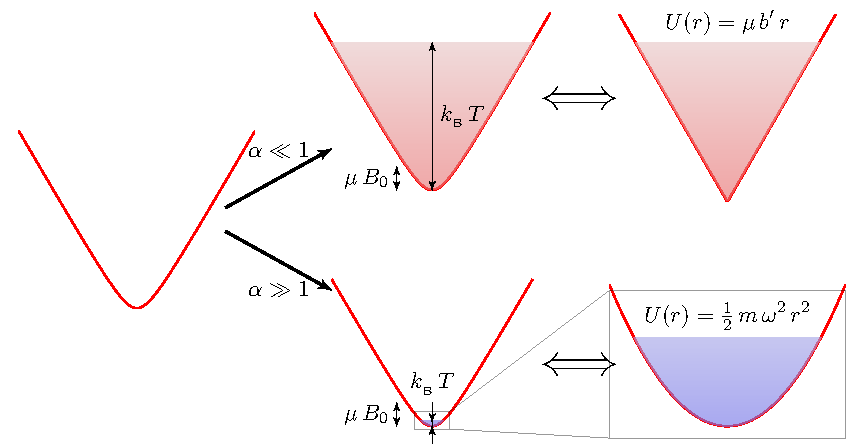
\includegraphics{P1/alpha}
\CaptionFigssss{Repr�sentation sch�matique du \ppt. Si la temp�rature du \jat est �lev�e (\ie: $\kb\,T \gg \mu\,\Bpara$), le potentiel hyperbolique peut �tre consid�r� comme �tant essentiellement lin�aire. Si � l'inverse sa temp�rature est faible (\ie: $\kb\,T \ll \mu\,\Bpara$), les atomes explorent essentiellement le fond du potentiel, que l'on peut alors consid�rer comme �tant harmonique.
}
\label{fig:alpha}
\efigh

%\AjouteLigne

\ApplicationNumerique
{Pour des conditions typiques de notre exp�rience, le \jat poss�de une temp�rature d'environ \microK{600}. Pour une valeur de champ longitudinal $\Bpara=\gauss{0.5}$, nous calculons le param�tre $\alpha \approx \val{0.025}$. Ceci traduit le fait que le jet est soumis � un \ppt essentiellement lin�aire.
L'extension transverse du jet dans le guide correspond typiquement � :
\RemonteUnPeuFig
\[
R \approx \frac{\kb\,T}{\mu\,\gradB} \approx \mm{0.25}
\pointformule
\RemonteUnPeuFig
\]
Dans un tel potentiel lin�aire, la p�riode d'oscillation radiale d'un atome d�pend de sa trajectoire, mais est typiquement de l'ordre de :
\RemonteUnPeuFig
\[
\tau \approx \sqrt{\frac{2\,R\,m}{\mu\,\gradB}} \approx \ms{1}
\pointformule
\]
\finformule
}

\casse

	\subsection{Guidage \ma d'un \jatuf}\label{sec:GuidageJet}
	Dans la sous-section pr�c�dente nous avons d�crit le potentiel $\Uhyp(r)$ auquel sont soumis les atomes de \Rb dans le \gm. Nous voulons maintenant discuter des caract�ristiques d'un \jat s'y propageant. Pour ce faire, nous allons consid�rer ici un \j � l'\eqthdy confin� radialement par le potentiel $\Uhyp(r)$. De plus, nous ne consid�rerons que le cas d'un jet supersonique dont la vitesse moyenne $\vjet$ %
\nome{\vjet}{Vitesse moyenne du jet se propageant selon l'axe $z$ du \gm}%
est \emph{plusieurs fois sup�rieure} � sa \dispvitlong $\deltavjet$. De cette mani�re, on s'assure que tous les atomes poss�dent une vitesse $\vz > 0$ %
%\nome{\vz}{Vitesse d'un atome selon l'axe $z$ du \gm}%
	suivant l'axe $z$ du \gm (on parle alors d'un jet \emph{monocin�tique} suivant l'axe $z$). En pratique, nous choisissons d'avoir:
$
	\vjet \geq 3\,\deltavjet
	\pointformule
$
	\subsubsection{Param�tres d�crivant le \jat}
En consid�rant le probl�me comme �tant invariant par translation suivant l'axe $z$, les seuls param�tres qui d�crivent le \jat confin� dans le potentiel hyperbolique $\Uhyp(r)$ sont:
%\Resultat{
%\paragraph{les param�tres du jet:}
	\begin{itemizel}
	\item la vitesse moyenne $\vjet$ du jet
	\item son \fat $\flux$,%
\nome{\flux}{Flux atomique du jet}%
	\item sa temp�rature $T$ d'�quilibre dans le r�f�rentiel en mouvement � la vitesse $\vjet$,
%\end{itemize}
%\paragraph{et les param�tres du confinement transverse:}
%	\begin{itemize}
	\item le gradient transverse $\gradB$ de \chm,
	\item le champ longitudinal $\Bpara$, ou de mani�re �quivalente, le param�tre $\alpha$ qui donne la forme du potentiel hyperbolique pour une temp�rature donn�e.
\end{itemizel}
%}
%
Ces 5 param�tres $(\vjet, \flux, T, \gradB, \alpha)$, relatifs � un jet � l'\eqthdy, permettent d'exprimer toutes les autres grandeurs physiques importantes qui doivent �tre prises en compte pour l'�tude du refroidissement par �vaporation:
%\Resultat{
\begin{itemizel}
	\item la \dat $\njet(r)$ du jet. Sa valeur maximale, sur l'axe $z$ du guide, est not�e $\njetaxe$, %
\nome{\njet(r),\njetaxe}{Densit� atomique du jet, et sa valeur maximale, sur l'axe $z$ du guide}%
	\item la \ddedpup $\rho(r)$ dont la valeur sur l'axe du guide est not� $\rhojetaxe$, %
\nome{\rho(r),\rhojetaxe}{Densit� dans l'\edp, et sa valeur maximale, sur l'axe $z$ du guide}% 
	\item le \tcolel moyen par atome $\gammacol$ au sein du jet, %
\nome{\gammacol}{Taux moyen de \colel par atome au sein du jet}%
	\item le \Ncolel moyen par atome $\Ncol$ tout au long de la propagation dans le \gm, %
\nome{\Ncol}{Nombre moyen de \colel par atome au sein du jet}%
	\item l'�nergie m�canique moyenne $\Emoy$ d'un atome du jet. %
\nome{\Emoy}{�nergie m�canique moyenne par atome au sein du jet}%
\end{itemizel}
%}
\EnFaitNon{
La \fdddedpup � l'\eqthdy est donn�e par la distribution de Boltzmann:
\[	\fjet(x,y,v_x,v_y,v_z) = C\,\Expo{-\frac{\Ham}{\kb\,T}} ,\]
o� $\Ham$ d�signe l'hamiltonien d'une particule qui s'exprime notamment gr�ce � la relation \vref{eq:PotentielTubesHyp}. Le facteur de normalisation $C$ sera choisi de mani�re � assurer que l'int�grale de $\fjet$ donne la \datlin suivant l'axe $z$ du guide. Nous pouvons donc �crire $\fjet$ sous cette forme:
\begin{align}
	\fjet(r,\vtrans, v_z)
	& = \frac{\flux}{\vjet} \, \fjetTrans(r, \vtrans) \, \fjetPara(\vz) \\
	\mbox{avec \quad} 
	& \fjetTrans(r, \vtrans)
	=  \Expo{-\frac{\mu\,\sqrt{\gradB^2\,r^2 + \Bpara^2}}{\kb\,T}} 
	 \, \Expo{-\frac{m\,\vtrans^2}{2\,\kb\,T}} \nonumber \\
  \mbox{et \quad} 
	& \fjetPara(\vz)
  = \Expo{-\frac{m\,\left(\vz-\vjet\right)^2}{2\,\kb\,T}}\nonumber 
	\label{eq:FjetBoltzmann}
\end{align}
MONOCINETIQUE ! ! ! 
}
\noindent Nous donnons ici l'expression de chacune de ces grandeurs~\cite{TTL}: 
\begin{subequations}
\begin{align}
	\njetaxe & = \frac{1}{2\,\pi}\,\frac{1}{1+\alpha}\,\frac{\flux}{\vjet}\,\left( \frac{\mu\,\gradB}{\kb\,T} \right)^2 
	\virguleformule 
	\label{eq:njetaxe}
	\\
	\rhojetaxe & \equiv \njetaxe \, \lambdaDB^3 = \frac{1}{2\,\pi}\,\frac{1}{1+\alpha}\,\frac{\flux}{\vjet}\,\left( \frac{\mu\,\gradB}{\kb\,T} \right)^2
	\,\, \frac{h^3}{(2\,\pi\,m\,\kb\,T)^{3/2}} 
	\virguleformule 
	\label{eq:rhojetaxe}
	\\
	\gammacol & = \frac{\sigma}{2\,\pi^{3/2}} \, \frac{1+2\,\alpha}{(1+\alpha)^2} 
	\, \frac{\flux}{\vjet} \, \left( \frac{\mu\,\gradB}{\kb\,T} \right)^2 
	\, \sqrt{\frac{\kb\,T}{m}} 
	\virguleformule 
	\label{eq:gammacol}
	\\
	\Ncol & \equiv \gammacol \, \frac{\Lguide}{\vjet} =
	\frac{\sigma}{2\,\pi^{3/2}} \, \frac{1+2\,\alpha}{(1+\alpha)^2} 
	\, \frac{\flux\,\Lguide}{\vjet^2} \, \left( \frac{\mu\,\gradB}{\kb\,T} \right)^2 
	\, \sqrt{\frac{\kb\,T}{m}} 
	\virguleformule 
	\label{eq:Ncol}
	\\
 	\Emoy & = \kb\,T\,\frac{2+\alpha}{1+\alpha} 
	\pointformule
	\label{eq:Emoy} 
\end{align}
\end{subequations}
Dans l'expression~\nref{eq:Emoy}, l'�nergie potentielle est prise comme �tant nulle au fond du pi�ge (en $r=0$) et $\sigma$ %
\nome{\sigma}{Section efficace de collision dans l'onde $s$}%
est la section efficace de collision dans l'onde $s$ (suppos�e ind�pendante de l'�nergie cin�tique des atomes).


\casse


Notons que les lois d'�chelles pour un confinement donn� permettent de mieux comprendre l'�volution des propri�t�s du \jatg en fonction des param�tres $(\vjet, \flux, T)$ que nous pouvons faire varier dynamiquement (voir la section \vref{sec:EvapRf}). 
\Resultat
{
Nous envisageons les deux cas limites:  $\alpha \ll 1$ (le potentiel ressenti par les atomes est essentiellement lin�aire) et $\alpha \gg 1$ (le potentiel ressenti par les atomes est essentiellement harmonique):
\newcommand{\grostruc}{\vphantom{$
{\dfrac{\flux^{{\vjet\,T^{\frac{3}{2}}}}
}{\vjet\,T^{\frac{3}{2}}_{{\vjet\,T^{{3}{2}}}}
}}$}}
\label{RQ:ProportionProprieteJet}
\begin{center}
\begin{large}
\begin{tabular}{rcc|cc}
\vphantom{${{{{{{{{{A^A}_A}_A}_A}_A}_A}_A}_A}_A}$} \qquad &  \qquad\qquad   
&  $\qquad \alpha \ll 1 \qquad$ & $ \qquad \alpha \gg 1 \qquad$ 
&\\
\cline{3-4}
\grostruc   $\njetaxe $& $\propto$   & $ \frac{\flux}{\vjet\,T^2} $ & $  \frac{\flux}{\vjet\,T} $ 
&\\
\cline{3-4}
\grostruc   $\rhojetaxe $ & $\propto$ & $ \frac{\flux}{\vjet\,T^{\frac{7}{2}}} $ & $  \frac{\flux}{\vjet\,T^{\frac{5}{2}}} $ 
&\\
\cline{3-4}
\grostruc   $\gammacol $ & $\propto$  & $ \frac{\flux}{\vjet\,T^{\frac{3}{2}}} $ & $  \frac{\flux}{\vjet\,\sqrt{T}} $ 
&\\
\cline{3-4}
\grostruc   $\Ncol $ & $\propto$  & $ \frac{\flux}{\vjet^2\,T^{\frac{3}{2}}} $ & $  \frac{\flux}{\vjet^2\,\sqrt{T}} $ 
&\\
\cline{3-4}
$\vphantom{T^{{\vjet\,T^{\frac{3}{2}}}}}$   $\Emoy $ & $=          $  & $ 2\,\kb\,T $ & $ \kb\,T $
&\\
\end{tabular}	
\end{large}
\end{center}
}
Il est donc clairement int�ressant de disposer d'un \jat intense, \uf est lent.

%\Resultat
%{\label{RQ:ProportionProprieteJet}
%\begin{center}
%\begin{large}
%\begin{tabular}{lccc}
%                  &     & ~ \qquad $ \alpha \ll 1$ \qquad ~ & $ \alpha \gg 1 $ 
%   \vspace{1ex}
%\\
%   $\njetaxe $& $\propto$   & $ \frac{\flux}{\vjet\,T^2} $ & $  \frac{\flux}{\vjet\,T} $ 
%   \vspace{1ex}
%\\
%   $\rhojetaxe $ & $\propto$ & $ \frac{\flux}{\vjet\,T^{\frac{7}{2}}} $ & $  \frac{\flux}{\vjet\,T^{\frac{5}{2}}} $ 
%   \vspace{1ex}
%\\
%   $\gammacol $ & $\propto$  & $ \frac{\flux}{\vjet\,T^{\frac{3}{2}}} $ & $  \frac{\flux}{\vjet\,\sqrt{T}} $ 
%   \vspace{1ex}
%\\
%   $\Ncol $ & $\propto$  & $ \frac{\flux}{\vjet^2\,T^{\frac{3}{2}}} $ & $  \frac{\flux}{\vjet^2\,\sqrt{T}} $ 
%   \vspace{1ex}
%\\
%   $\Emoy $ & $=          $  & $ 2\,\kb\,T $ & $ \kb\,T $ \\
%\end{tabular}	
%\end{large}
%\end{center}
%}



\section{De l'injection puls�e de \pats � l'obtention d'un \j continu}\label{sec:FormationJetContinu}
Cette section pr�sente la technique utilis�e pour produire un \jatuf et intense dans le \gm. 

	\subsection{Pourquoi une injection puls�e?}
L'�quipe de \dgo, dans laquelle j'ai effectu� ma th�se, est la premi�re � avoir r�alis� le guidage d'un \jaf~\cite{CRA02}. Deux techniques exp�rimentales diff�rentes ont �t� mises au point afin de produire ce jet en couplant les atomes d'un \pmo � un \gm:
\begin{itemizel}
	\item la premi�re consiste � \emph{injecter en continu} les atomes. Pour ce faire, le pi�geage magn�to-optique est r�alis� uniquement suivant les deux directions transverses. Suivant l'axe du guide, les atomes \emph{fuient} vers l'entr�e du guide gr�ce une technique de m�lasse mouvante. Notons que, l'injection �tant continue, il n'est pas possible d'optimiser simultan�ment la capture des atomes et leur lancement. 
	\item la deuxi�me repose sur \emph{l'injection puls�e de \pats}. La \dispvitlong des \pats se propageant dans le guide induit un �talement suivant l'axe du \gm. Le recouvrement de ces \ps permet ainsi la formation d'un \jat continu, apr�s une distance de propagation de typiquement \cm{50}.
\end{itemizel} 


\casse


Ces deux m�thodes d'injection donnaient alors des performances similaires en terme de flux ($\approx \atparsec{3E8}$) du \jat. En revanche, sa temp�rature �tait dix fois inf�rieure en utilisant la deuxi�me technique ($\approx \microK{100}$)~\cite{RCL03}. Cela est principalement d� � deux raisons:
	\begin{itemize}
	\item le contr�le dynamique des param�tres du \pmo permet de combiner un tr�s bon taux de capture, suivi d'un refroidissement tr�s efficace par une technique de m�lasse optique.% (se reporter � la section \vref{sec:EtapesRefroidissement}).
	\item la pr�sence en continu d'un \pmo d�truit partiellement le \jgm du fait de la diffusion de lumi�re sur la transition \termetech{repompeur} (les atomes sont en effet pr�par�s dans l'�tat $\EtatSFmF{1}{-1}$). L'injection puls�e permet quant � elle, apr�s l'injection, de laisser chaque \p s'�loigner dans le guide avant de charger le \p suivant. Le \fat moyen observ� est plus important%
	\footnote{Le \fat est, dans le cas de l'injection puls�e, une fonction croissante de la distance entre deux \pss: plus la distance qui s�pare le \pmo du \p pr�c�demment inject� est grande, moins la lumi�re \termetech{repompeur} affectera celui-ci.} quand on utilise une injection puls�e.
\end{itemize}

	\subsection{Formation de \pats ultra-froids}\label{sec:PaquetsPmo}
Nous rappelons ici bri�vement les choix retenus pour une alimentation optimale du \pmo. 
%d�crivons ici la mani�re dont les \pats sont obtenus. 
La figure~\nref{fig:VueEnsembleSetupJet} repr�sente une vue d'ensemble du \setup. Les diff�rents �l�ments qui le constituent sont d�taill�s dans le chapitre 2 de la th�se de T.~Lahaye~\cite{TTL}. 
Nous donnerons donc simplement les param�tres importants qui caract�risent les principales parties de notre \setup:
	\begin{itemize}
	\item \textbf{un four � recirculation%
	\footnote{La d�nomination de \termetech{four} provient du fait qu'un �chantillons de rubidium solide est chauff� (� typiquement \val{100}-\SI{150}{\degreecelsius}), et ce afin d'augmenter sa pression de vapeur saturante. Le four est ainsi empli d'une vapeur de rubidium, qui s'�chappe dans le syst�me � \uv pour alimenter le \pmo. La d�nomination de \termetech{four � recirculation} provient du fait que la g�om�trie du four permet de r�cup�rer automatiquement une partie du rubidium inutilis�. Ceci permet d'augmenter consid�rablement la dur�e d'utilisation du four~\cite{TTL}.}%
} dont la conception est inspir�e de la r�f�rence~\cite{CaP78} fournit un jet collimat� d'atomes de \Rb avec un flux d'environ $\atparsec{2E12}$ et une vitesse moyenne de l'ordre de \mps{400}.
	\item \textbf{un \ZS}\cite{PhM82,PPM82,PMP85} d'un m�tre de long ralentit $10\%$ des atomes provenant du four � une vitesse moyenne de l'ordre de \mps{20}. Le flux obtenu, d'environ $\atparsec{2E{11}}$, fait de ce \ZS l'un des plus performants au monde.
	\item \textbf{un \pmo de g�om�trie allong�e} capture une partie des atomes ralentis par le \ZS. Le taux de capture est d'environ $\atparsec{2E10}$. Le nombre d'atomes sature rapidement ($\approx\seconde{1}$) � environ $\val{E10}$ atomes. Notons que ce taux de chargement est nettement sup�rieur � ceux observ�s dans les exp�riences typiques de \condbe.
\end{itemize}
%
\bfigh
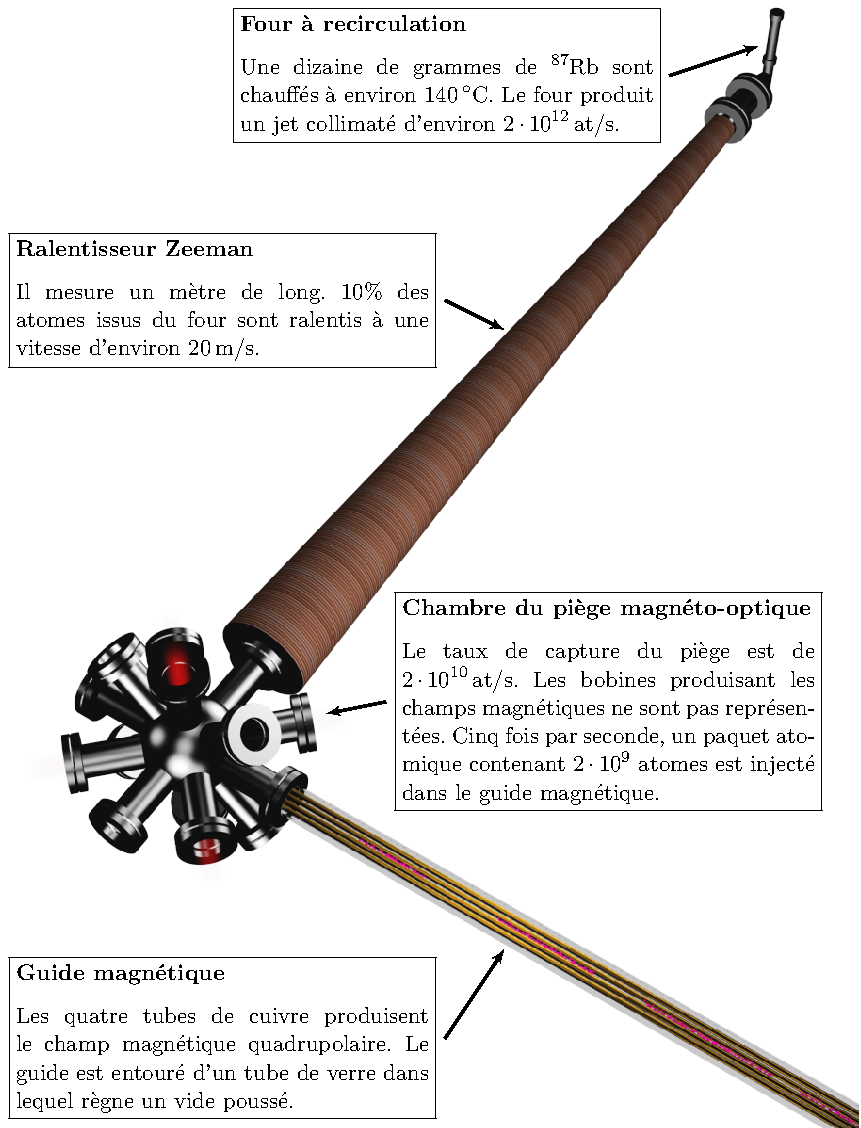
\includegraphics{P1/VueEnsembleSetupJet}
\CaptionFig{Sch�ma repr�sentant une vue d'ensemble du \setup. 
}
\label{fig:VueEnsembleSetupJet}
\efigh
%
\Resultat{
Gr�ce � ce \setup, il nous est ainsi possible de produire un \pat contenant typiquement  $\Npat = \val{2E9}$ atomes en $\ms{100}$.
}
La temp�rature d'un tel \pat captur� dans le \pmo d�pend de plusieurs facteurs (d�saccord des lasers, nombre d'atomes, gradient de \chm,...), mais ce situe typiquement dans la plage \val{100}-\microK{200}. Une phase de m�lasse optique permet d'obtenir une temp�rature d'environ \val{20}-\microK{30}.


\casse


	\subsection{Technique d'injection dans le \gm}\label{sec:InjectionGuide}
	Le couplage des atomes du \pmo dans le \gm est une �tape d�licate. De mani�re � mettre en mouvement le \pat, nous utilisons une technique de \emph{m�lasse mouvante}%, qui fut initialement d�velopp�e dans le contexte des horloges atomiques � fontaine d'atome froids 
~\cite{CSG91}. La mise en \oe uvre de cette technique dans le \setup, ainsi que les d�tails relatifs au pompage optique des atomes dans l'�tat pi�g� \EtatFmF{1}{-1} et au guidage des \ps vers l'entr�e du \gm, sont d�taill�s dans la th�se de T.~Lahaye~\cite{TTL}.
Nous nous contenterons ici de mentionner les quatre �tapes de notre \seqexp qui est r�p�t�e environ 5 fois par seconde:
\begin{enumerate}
	\item Capture dans le \pmo pendant \ms{100} d'atomes issus du \ZS : les lasers du \pmo sont d�saccord�s de $\delta=-3\,\Gamma$ et les gradients de \chm valent typiquement \gausspcm{5} transversalement et \gausspcm{0.5} selon l'axe longitudinal.
	\item \termetech{M�lasse optique mouvante} de \ms{3}. Le d�saccord des lasers est alors:
	\begin{itemize}
		\item gard� constant � $\delta=-3\,\Gamma$ pendant \ms{1.5},
		\item puis augment� lin�airement jusqu'� $\delta=-12\,\Gamma$ en \ms{1.5}.
	\end{itemize}
	\item \termetech{Pompage optique} (pendant \ms{0.7}) dans le \snZ $\EtatSFmF{1}{-1}$.
	\item \termetech{Pr�-guidage \ma} du \pat pendant environ \ms{100}. Cette phase consiste � pr�venir l'expansion transverse ainsi que la chute libre du \p avant son arriv�e dans le guide dont l'entr�e est situ�e � \cm{5} du \pmo. En pratique, un \gtchm d'environ \gausspcm{100} est produit par les bobines du \pmo.
\end{enumerate}
%
\Resultat{
L'optimisation de cette proc�dure lors de la premi�re ann�e de ma th�se a permis de produire un \jatg dont les caract�ristiques $(\vjet, \flux, T)$ sont:
\begin{itemize}
	\item $\vjet = \cmps{60}$ (voir la remarque \vpageref[ci-dessous]{Rq:InjectionPente}),
	\item $\flux = \atparsec{7E9}$,
	\item $T = \microK{600}$.
\end{itemize}
}
Ces param�tres sont obtenus pour un confinement caract�ris� par un \gtchm $\gradB = \gausspcm{800}$ et un champ longitudinal $\Bpara = \gauss{0.5}$. Le param�tre $\alpha=\ttfrac{\mu\,\Bpara}{\kb\,T}$ vaut dans ces conditions $\alpha = \val{0.025}$, traduisant le fait que le jet est soumis � un \ppt essentiellement lin�aire (voir la \autoref{sec:ConfigMagnetiqueGuide}).
%
\ApplicationNumerique{
Calculons, gr�ce aux expressions \vrefrange{eq:njetaxe}{eq:gammacol}, les autres caract�ristiques du jet pour les valeurs �nonc�es ci-dessus:
\begin{itemize}
	\item \dat sur l'axe $z$: $\njetaxe = \atpcc{3.6E10}$,%3,6125
	\item \ddedpup sur l'axe $z$: $\rhojetaxe = \val{1.7E{-8}}$,%1,694
	\item $\gammacol = \val{3.6}$ collisions par seconde et par atome.%3,580
	\item $\Ncol \approx 20$ collisions tout au long de la propagation dans le \gm.
\end{itemize}
}

\casse


\subsubsection{Utilisation d'une \secpent pour ralentir le jet}
{\label{Rq:InjectionPente}
Notons que la vitesse d'injection des \pats est $\vinj = \cmps{90}$. La vitesse du jet $\vjet = \cmps{60}$ est obtenue par la mise en place d'une \secpent, ayant un d�nivel� de \mm{22} sur les premiers \m{1.7} du \gm (voir la figure \vref{fig:Montage10Antennes}).
On peut se demander quel est l'avantage � effectuer cette proc�dure de ralentissement sachant qu'il est techniquement possible de communiquer une vitesse initiale $\vinj = \cmps{60}$ aux \ps. 

La raison en est, comme nous l'avons �voqu� pr�c�demment, que le \fat est d'autant plus �lev� que la distance qui s�pare le \pmo du \p pr�c�demment inject� est grande (� cause de la lumi�re repompeur diffus�e par le \pmo). Le fait d'injecter les \ps � une vitesse relativement �lev�e permet d'augmenter cette distance (pour un taux de r�p�tition donn�), et donc d'augmenter le \fat. 

En revanche, les expressions \vrefrange{eq:njetaxe}{eq:gammacol}, montrent que nous avons tout int�r�t � disposer d'un jet le plus lent possible. La proc�dure de ralentissement est donc un moyen de combiner un flux �lev� � une vitesse faible. 
}


\subsection{Entr�e non-adiabatique du jet dans le \gm}\label{sec:EntreeGuideNonAdiabatique}

�tant donn�e la temp�rature du \nat durant la phase de m�lasse optique (soit typiquement \val{20}-\microK{50}), on peut se demander pourquoi le jet poss�de une temp�rature si �lev�e (\microK{600}). Ceci est d� au fait que chaque nuage, subit une \emph{compression transverse} non-adiabatique lors de l'allumage du pr�-guide, ainsi qu'� l'entr�e du \gm. L'�nergie fournie au nuage est d'autant plus �lev�e que son extension transverse est grande\footnotemark. 
%Nous verrons d'ailleurs dans le chapitre~\nref{chap:MiroirMobile}, que la \dispvitlong d'un \p individuel dans le \gm n'est que de 
\footnotetext{Plus l'extension transverse du nuage est faible, moins il sera sensible � une augmentation de la force de confinement. D'ailleurs, si on imagine un ensemble d'atomes r�unis sur l'axe $z$ du \gm, ceux-ci se propageant selon une ligne de \chm nul seront insensible � l'augmentation du \gtchm.}
\ApplicationNumerique
{
On peut estimer l'ordre de grandeur de l'�chauffement en consid�rant l'extension transverse d'un nuage, $2\,r\approx\mm{1}$ et le \gtchm du guide, $\gradB \approx \gausspcm{800}$. Lors de l'entr�e non-adiabatique des atomes dans le guide, ceux-ci vont se voir fournir une �nergie potentielle moyenne de l'ordre de:~$\mu\,\gradB\,r$, qui correspond � $\kb\times\milliK{2}$.
Les collisions entre atomes vont cependant conduire � une redistribution de l'�nergie sur les autres degr�s de libert�s et la temp�rature d'�quilibre du jet n'augmentera finalement que de typiquement\footnotemark~\milliK{1}.
}
\footnotetext{La fraction d'�nergie qui se r�partit sur chaque degr�s de libert� des atomes fait intervenir le th�or�me du viriel et est expos� dans la remarque \vpageref{Rq:Viriel}.}

\ifthenelse{\FormatEUE > 0}{}
{\AjouteLigne}
\RemonteUnPeuFig\RemonteUnPeuFig\RemonteUnPeuFig
\subsubsection{Temp�rature longitudinale des \ps individuels}
Dans le chapitre~\nref{chap:MiroirMobile}, nous serons amen�s � consid�rer la propagation libre de \pats individuels dans le \gm. Nous y montrerons que, par une technique de \termetech{temps de vol}, on peut mesurer la \dispvitlong $\Tlong$ d'un \p. Il est int�ressant de mentionner d�s maintenant, que celle-ci est typiquement de seulement $\Tlong=\microK{150}$ (dans les conditions habituelles de fonctionnement).

\noindent Pourquoi la \templong $\Tlong$ d'un \p se propageant dans le guide est elle inf�rieure � la temp�rature d'�quilibre ($T=\Tlong\approx\microK{600}$) du jet, qui n'est finalement que le produit du recouvrement d'une succession de \ps ?

\noindent Cette observation s'explique par le fait que le \tcolel au sein d'un \pat libre chute tr�s rapidement � cause de l'�talement spatial de ce dernier. Ceci a pour cons�quence de \sotosay{geler} la \reth entre les degr�s de libert� transverses et longitudinaux. 
Ainsi, m�me si la \tempt d'un \p est de l'ordre de \microK{800} du fait de la compression lors de l'entr�e non-adiabatique dans le \gm, il y a trop peu de collisions par atome pour atteindre un \eqthdy local.
\ApplicationNumerique{
On peut estimer le nombre moyen de collisions par atome pour un \p en propagation libre dans le guide. 

Nous avons d�j� estim� le nombre $\Ncol \approx 20$ de collisions tout au long de la propagation du jet dans le \gm. Or, pour former le jet, il y a en permanence environ \val{20} \ps dans le guide (l'injection est faite $5$ fois par seconde et la propagation dure $\approx\seconde{4}$). 

On peut donc estimer le nombre moyen de collisions par atome pour un seul \p � $\ttfrac{\Ncol}{20}\approx 1$. Ceci est insuffisant pour �tablir un \eqthdy local~\cite{LaG06}.
}



\section{Caract�risation du \jat} \label{sec:MesureJat}

Cette section d�crit les diff�rentes techniques qui nous permettent de caract�riser le \jatg produit gr�ce � notre \setup. Nous avons vu dans la section~\nref{sec:GuidageJet} que les trois param�tres importants qui caract�risent le jet sont sa vitesse moyenne $\vjet$, son \fat $\flux$, et sa temp�rature $T$.% d'�quilibre dans le r�f�rentiel en mouvement � la vitesse $\vjet$. 

La vitesse du jet est a priori connue puisque la vitesse d'injection $\vinj$ est impos�e de mani�re contr�l�e lors de la phase de m�lasse mouvante. Connaissant le d�nivel� $\Hpente$ de la \secpent, nous pouvons calculer la vitesse du jet.%
\footnote{Nous pouvons aussi mesurer exp�rimentalement la vitesse du \jat en utilisant une technique de \termetech{temps de vol longitudinal}~\cite{TTL}.} 
% : $\vjet = \vinj$. 
Connaissant la vitesse moyenne du jet, le flux atomique se d�duit d'une mesure pr�cise de la \datlin. 

Dans cette section, nous allons aborder le probl�me de la mesure de la \dat, puis nous d�taillerons le protocole de mesure de la temp�rature du \j.


%Toutes les mesures quantitatives que nous effectuons pour d�terminer ces 3 grandeurs sont  bas�e sur une mesure pr�cise de la \datlin dans le \gm. 
%Si d�tecter la pr�sence d'atomes lors de leur propagation dans le \gm est une chose ais�e, obtenir des mesures quantitatives quant au flux et � la \datlin est plus d�licat. 

%	\subsection{Mesure de \templong}
%Dans le cadre de l'�tude de l'\rpef du \jat dont nous disposons, il est utile d'avoir acc�s de mani�re exp�rimentale au caract�re \emph{hors d'\eqthdy} du jet. Ayant une m�thode fiable de mesure de la temp�rature transverse $\Ttrans$ du jet, nous avons d�velopp� lors de ma premi�re ann�e de th�se une technique de mesure de la temp�rature longitudinale $\Tlong$ du \jat. En effet, dans une situation de mise hors d'\eqthdy, la \tempt et la \templong ne sont pas forcement �gales. l'�tude de la \reth du \jat passe donc par la comparaison des deux temp�ratures mentionn�es.
%La mesure de temp�rature longitudinale est effectu�e par une technique de temps de vol. Pour cela nous proc�dons de la mani�re suivante:
%\begin{itemize}	
%\item � l'endroit du guide o� nous d�sirons effectuer la mesure, le \jat est localement d�truit gr�ce � un faisceau laser \sotosay{pousseur} qui d�vie les atomes hors du \gm. 	
%\item � l'instant d�finit comme �tant $t=0$, le laser pousseur est arr�t�, et le jet reprend sa propagation libre dans le guide.	
%\item Quelques dizaine de centim�tres plus loin, le flux atomiques est mesur� en fonction du temps. La fonction 
%\end{itemize}

\subsection{Mesure de la \datlin et du flux dans le guide}\label{sec:MesureDensiteGuide}
La technique utilis�e pour effectuer les mesures de \datlin dans le \gm repose sur l'absorption d'un faisceau laser coupant la trajectoire du \jat. 

\subsubsection{Mesure d'absorption sur une transition cyclante}
Une possibilit� envisag�e alors est de r�aliser l'absorption du faisceau laser dont la fr�quence est verrouill�e sur la la transition cyclante \TransCycle. Cette technique%
\footnote{Une technique qui rappelle d'ailleurs l'imagerie par absorption habituellement utilis�e pour des nuages d'atomes (voir le chapitre~\nref{chap:Imagerie}).% De mani�re � fonctionner correctement, il faut superposer au laser excitant la transition cyclante un laser \termetech{repompeur}.
} 
souffre d'un inconv�nient majeur : celui d'�tre tr�s sensible au d�saccord en fr�quence du laser par rapport � la r�sonance. Or, les gradients de \chm sont tr�s importants dans la r�gion o� les atomes sont confin�s. Ceci implique un �largissement inhomog�ne de la raie spectrale due � l'effet Zeeman.
\ApplicationNumeriqueTitre{�largissement inhomog�ne par effet Zeeman}{
�valuons l'importance de cet �largissement pour un \jat typique confin� dans le \gm, sachant que:
\begin{itemize}
	\item la temp�rature du jet peut typiquement atteindre \microK{600}. Ce qui correspond � une extension transverse $R$ dans le guide de l'ordre du millim�tre.
	\item le gradient transverse $\gradB$ de \chm pouvant atteindre \SI{1}{\kilo G \per\centi\meter}, le module du champ \sotosay{explor�} par les atomes du jet varie sur une plage $\Delta B$ de l'ordre de $R\,\gradB = \SI{100}{G}.$
\end{itemize}
Ainsi, l'effet Zeeman correspondant implique un �largissement inhomog�ne $\Delta \nu$ d�fini par :
\[
\Delta\nu = \frac{\mu\,\Delta B}{2\,\pi\,\hbar} \approx \SI{70}{\mega\hertz}
\pointformule
\]
\finformule
}
Cette valeur est � comparer avec la largeur spectrale d'un laser verrouill� en fr�quence sur la transition cyclante, typiquement inf�rieure � \SI{1}{\mega\hertz}. 
Il est donc hors de question de n�gliger cet effet. M�me avec une temp�rature de \jat dix fois inf�rieure � la valeur consid�r�e ici, n�gliger l'�largissement d� au gradient de \chm se traduirait par une mesure erron�e du nombre d'atomes participant � l'absorption du faisceau.

\subsubsection{Mesure d'absorption sur une transition ouverte}\label{sec:MesureDensiteGuideOuvert}
\ifthenelse{\FormatEUE > 0}{}
{\AjouteLigne}
%\AjouteLigne
Au lieu d'utiliser la transition cyclante, nous �tudions l'absorption du \jat sur la transition ouverte $\TransOpen$. 
C'est cette transition qui est habituellement utilis�e pour \termetech{repomper} les atomes dans l'�tat \EtatSF{2} dans un \pmo.

%\Resultat
{
La probabilit� qu'a un atome d'absorber un photon sur cette transition d�pend certes du d�saccord du laser, et donc de l'�largissement inhomog�ne d� au gradient de \chm. Cependant, le caract�re ouvert de cette transition conf�re � cette m�thode une grande robustesse. Un atome pr�par� dans l'�tat \EtatSF{1} et excit� sur cette transition, ne peut absorber, en moyenne, que $2$ photons avant de tomber dans l'�tat \EtatSF{2}, �tat qui n'est plus sensible � la lumi�re du laser sonde (voir la \autoref{sec:ImagerieFun}).
}	
%Ainsi, si l'intensit� du laser sonde est suffisante, chaque atome absorbera deux photons (en moyenne) et ce, m�me en pr�sence d'un �largissement inhomog�ne. 

En pratique, la fr�quence du laser sonde est balay�e 70 fois par seconde autour de la transition $\TransOpen$ sur une plage d'environ \SI{1}{\giga\hertz}. L'absorption du faisceau est mesur�e par une photodiode et on observe un pic d'absorption au moment o� la fr�quence du laser passe � r�sonance. La mesure de l'aire du pic d'absorption permet de d�terminer le nombre d'atomes qui se trouvent dans le faisceau laser � ce moment pr�cis.% (2 photons absorb�s par atome en moyenne). 
\vspace{0.2cm}
\inlinefig{\begin{overpic}[width=7cm, unit=1cm]{P1/SondeGuide}
\tikz\draw[-latex', color=white, line width = 0.2cm] (0,0) ++ (0.1,1.00) -- ++(1.6,1);
\tikz\draw[latex'-latex', color=white] (0,0) ++ (4,4.5) -- ++(-1.1,0.25) node[pos=0.5, above]{$D$};
\end{overpic}} 
Ci-contre, nous repr�sentons de mani�re sch�matique le faisceau sonde coupant le \j ainsi que l'ombre port�e au moment de l'absorption. Le \jat �tant transversalement plus petit que le faisceau du laser sonde, le nombre $N$ d'atomes qui participent � l'absorption est d�termin� par le diam�tre $D$ du faisceau. $D$ correspond en effet � la longueur sur laquelle le jet est �clair�. Nous pouvons donc d�duire la \datlin:
\[
n_z=\frac{N}{D}
\pointformule
\]
\`A partir de la connaissance de la vitesse moyenne $\vjet$ nous d�duison le \fat $\flux$.  
Cette technique s'av�re �tre tr�s peu sensible au gradient de \chm du guide.


\casse


\subsection{Mesure de la \tempt du jet}\label{sec:MesureTempTrans}
Commen�ons par d�finir la \emph{\tempt}, not�e $\Ttrans$, %
\nome{\Ttrans}{Temp�rature transverse du \jat}%
qui correspond � l'�nergie thermique distribu�e sur les degr�s de libert� perpendiculaires � l'axe du \gm. Il est en effet important de diff�rencier $\Ttrans$ de la temp�rature $T$ � partir du moment o� nous voulons �tudier les propri�t�s d'un jet mis hors d'\eqthdy.

La mesure de \tempt du \jat rel�ve d'une technique de spectroscopie \rf originale d�velopp�e, avant que je ne d�bute ma th�se, par \dgo%
\footnote{Cette technique a d'ailleurs depuis �t� adapt�e dans d'autres groupes afin d'analyser des \becs\cite{FGW07}).}%
. 
La description d�taill�e de celle-ci fait l'objet du chapitre 3 de la th�se de T.~Lahaye~\cite{TTL}. Nous allons ici rappeler le principe de cette m�thode.

	\subsubsection{Principe de la m�thode: le \fispse}
	En pr�sence d'un \chm, et � l'aide d'une onde \rf, il est possible d'induire des transitions atomiques entre \snZs. Pour un nuage d'atomes immerg�s dans un \chm uniforme de module $B$, on peut exprimer la fr�quence $\nurf$ de l'onde n�cessaire pour effectuer cette transition:%
\nome{\nurf}{Radio-fr�quence passer d'un �tat magn�tiquement pi�g�, � un �tat non-pi�g�}%
\begin{equation}
	\nurf(B) = \frac{\mu\,B}{2\,\pi\,\hbar}.
	\label{eq:nurfB}
\end{equation}
Dans le cas d'un nuage pi�g� magn�tiquement, le champ $B$ n'est pas uniforme sur toute l'extension du nuage. Nous sommes donc en pr�sence d'un �largissement inhomog�ne de la transition, \cad que, pour une fr�quence $\nurf$ donn�e, \emph{seuls certains atomes} v�rifieront la condition~\nref{eq:nurfB} et pourront effectuer la transition $\EtatFmF{1}{-1} \rightarrow \EtatFmF{1}{0,+1}$, passant d'un �tat magn�tiquement pi�g�, � un �tat non-pi�g�.% (voir la \autoref{sec:PiegeageMagnetique}). 

La figure~\nref{fig:MesureTempTrans} montre de mani�re sch�matique que dans le cas du confinement $\Uhyp(r)$ impos� par notre \gm, une fr�quence donn�e $\nurf$ va correspondre � certains atomes, situ�s � une distance $\Rnurf$ de l'axe du \gm. 

\bfig
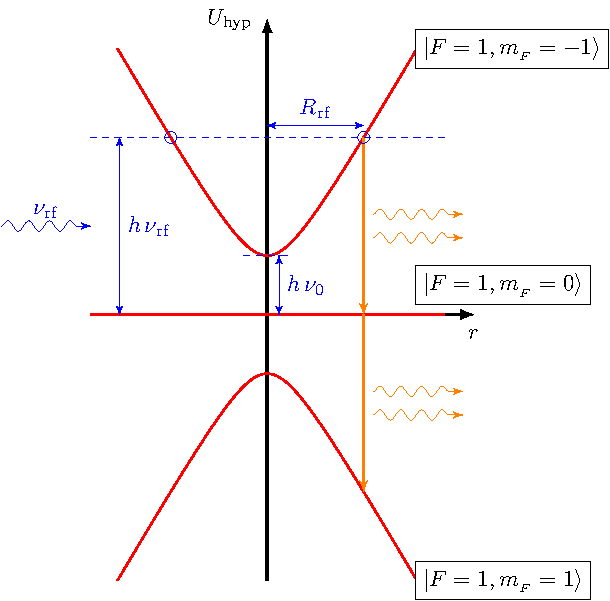
\includegraphics{P1/MesureTempTrans}
\CaptionFig{Repr�sentation sch�matique des transitions entre \snZs pour des atomes soumis � une onde \rf. La situation consid�r�e ici est celle correspondant au potentiel de pi�geage magn�tique � sym�trie cylindrique d�crit dans la \autoref{sec:PiegeageMagnetiqueGuide}.
Les atomes, initialement dans l'�tat \EtatFmF{1}{-1}, peuvent effectuer une transition stimul�e vers un �tat non-pi�g�. Ceci ne peut toutefois se produire qu'� la condition de v�rifier la relation de r�sonance $ h\,\nurf = \Uhyp(r) $.
La fr�quence $\nurf$ d�finit ainsi un cylindre de rayon $\Rnurf$. Les atomes qui traversent cette surface durant leur �volution deviennent non-pi�g�s et sont perdus. La \rf correspondant � un cylindre de rayon nul est not�e $\nu_0$ sur le sch�ma.}
\label{fig:MesureTempTrans}
\efig

La fr�quence $\nurf$ d�finit ainsi un cylindre de rayon $\Rnurf$%
\nome{\Rnurf}{Rayon du cylindre de \fisp}%
. Les atomes qui traversent cette surface durant leur �volution deviennent non-pi�g�s et sont perdus. 
La longueur de ce cylindre (suivant l'axe du guide) correspond � la port�e $\Lantenne$ %
\nome{\Lantenne}{Port�e selon l'axe du \gm de l'antenne de \fisp}%
de l'antenne \rf suivant l'axe du \gm et vaut typiquement \cm{20} dans notre cas (ce point est d�taill� dans la \autoref{sec:EvapRf}). 
%
\Resultat{\label{Rq:CritereFiltrage}
�liminer des atomes du jet par application d'une \rf correspond a un \emph{filtrage spatial s�lectif}. 
Le crit�re permettant de d�terminer si un atome va �tre �limin� ou non du jet est un porte sur la trajectoire de l'atome: 
si celle-ci coupe la surface du cylindre de rayon $\Rnurf$ d�fini par la \rf $\nurf$, l'atome est �limin� du jet. 
}

\casse

La figure~\nref{fig:TrajGuide} illustre la s�lectivit� de ce crit�re par des exemples de trajectoires atomiques dans le plan $(x,y)$.
Notons que le crit�re de filtrage spatial n'est pas seulement li� � l'�nergie m�canique transverse $\Etrans$ de l'atome. Il porte en fait sur le couple $(\Etrans, \Lz)$, o� $\Lz$ est le moment cin�tique de l'atome autour de l'axe du \gm.
%
\bfigh
\vspace{-.5cm}
\subfloat[]
{\label{TrajGuide_a}
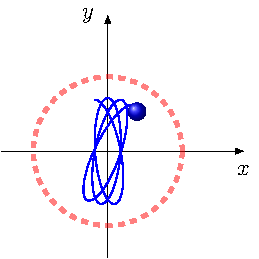
\includegraphics{P1/TrajGuide_a}
}
\subfloat[]
{\label{TrajGuide_c}
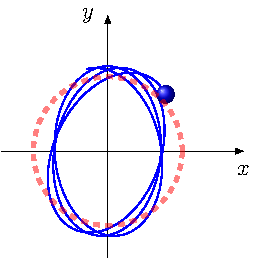
\includegraphics{P1/TrajGuide_c}
}
\subfloat[]
{\label{TrajGuide_b}
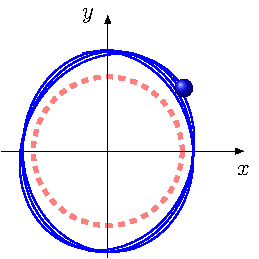
\includegraphics{P1/TrajGuide_b}
}
\CaptionFig{Repr�sentation dans le plan transverse $\xy$ de trajectoires atomiques typiques dans le potentiel de \cthyp $\Uhyp(x,y)$. La pr�sence d'une \rf $\nurf$ d�finit un cylindre de rayon $r=\Rnurf$. Tout atome traversant la surface de ce cylindre change de \snZ, et est �limin� du jet. La trajectoire (a) correspond � un atome qui ne sera pas �limin� car l'atome n'atteint jamais le rayon $\Rnurf$. L'atome ayant la trajectoire (b) sera �limin� puisque celle-ci coupe le cylindre de filtrage. Notons qu'un atome ayant la trajectoire (c) ne sera pas �limin� malgr� le fait que son �nergie m�canique est relativement �lev�e (l'atome orbite en permanence � l'ext�rieur du cylindre).}
\label{fig:TrajGuide}
\efigh

%\Remarque
{
Dans le cas o� le \jat soumis � l'onde \rf est � l'\eqthdy, il est commode d'introduire le \emph{param�tre de filtrage} sans dimension $\eta$ %
\nome{\eta}{Param�tre sans dimension d�crivant le \fisp du jet}%
d�fini comme suit:
\begin{equation}
	\eta
	 \equiv \frac{\Uhyp\left( \larger{\Rnurf}\Rnurf \right) - \Uhyp\left( \larger{\Rnurf} 0 \right) }{\kb\,\Ttrans}
	 = \etaexpr,
	\label{eq:Eta}
\end{equation}
%o� $\nu_0$ est la fr�quence qui correspond � un filtrage de particule sur un cylindre de rayon nul (par definition, $h\,\nu_0 \equiv \mu\,\Bpara$, voir figure~\nref{fig:MesureTempTrans}).\\
Ce param�tre $\eta$ est d�fini par le rapport des deux �nergies en jeu lors du \firf :
\begin{itemize}
	\item l'�nergie potentielle $\Uhyp(\Rnurf)-\Uhyp\left( 0 \right)$ qui correspond � la surface du cylindre de filtrage,
	\item l'�nergie thermique transverse moyenne $\kb\,\Ttrans$ des atomes du jet.
\end{itemize} }


		\subsubsection{Exploitation quantitative d'un \spfirf}
		La m�thode spectroscopique de d�termination de la \tempt repose sur la mesure du \fat apr�s une zone de filtrage s�lectif induit par une antenne \rf. 
La figure~\nref{fig:SpectreEvap} donne un exemple de courbe obtenue quand, pour un flux incident $\flux$ donn�, on mesure le flux $\fluxapres$ d'atomes qui restent apr�s passage au travers de la zone de \fisp , en fonction de la \rf $\nurf$ utilis�e pour effectuer le filtrage. La grandeur pertinente � prendre en compte est en fait le rapport des flux :%
\nome{\rapflux(\nurf)}{Fraction du flux restant apr�s l'action dune zone de \fisp}%
\begin{equation}
	\rapflux(\nurf) \equiv \frac{\left.\fluxapres\right|_{\nurf}}{\flux}
	\label{eq:rapportflux}
\end{equation}
On appellera ce type de courbe exp�rimentale un \emph{\spfirf}, ou plus simplement, un \termetech{\spfi}. \`A partir de ces donn�es, et en connaissant les caract�ristiques du confinement, il est possible de d�terminer la \tempt d'un jet suppos� � l'\eqthdy.

\pagebreak

\bfighss
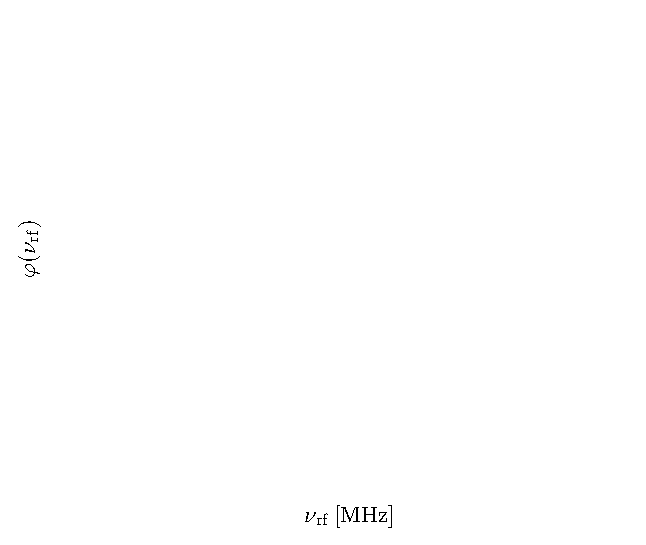
\includegraphics{P1/WithoutEvap}
\CaptionFigsss{Mesure du rapport des \fats avant, et apr�s filtrage spatial du jet en fonction de la \rf $\nurf$ utilis�e. Une telle courbe est caract�ristique de la distribution transverse $(\Etrans, \Lz)$ d'un \jat � l'\eqthdy. Pour ces donn�es exp�rimentales, le \ppt est lin�aire ($\Bpara=0$), et le \gtchm est $\gradB = \gausspcm{600}$.
}
\label{fig:SpectreEvap}
\efigh

%\Intuition
{
On comprend le comportement asymptotique de la courbe repr�sent�e sur la figure~\nref{fig:SpectreEvap}:
\begin{itemize}
	\item pour $\nurf \rightarrow \nu_0$, \cad pour $\eta \rightarrow 0$, le rayon du cylindre de filtrage $\Rnurf$ devient tr�s petit devant l'extension transverse du jet. Les atomes �limin�s sont ceux qui passent � proximit� imm�diate de l'axe du \gm. Le nombre d'atomes concern�s est d'autant plus faible que le rayon $\Rnurf$ est petit. Pour un rayon nul, aucun atome n'est �llimin� et nous avons donc :
	\[ 
	\rapflux(\eta \rightarrow 0) = 1 
	\pointformule
	\]
	\item pour $\nurf \rightarrow \infty$, \cad pour $\eta \rightarrow \infty$, le cylindre de filtrage contient tous les atomes, et aucun ne traverse sa surface:%. Tous les atomes sont conserv�s :
	\[ 
	\rapflux(\eta \rightarrow \infty) = 1 
	\pointformule 
	\]
	\item par ailleurs, la largeur de cette courbe est directement li�e � la temp�rature du jet. En effet, si des atomes sont �limin�s sur une large plage de \rf, cela traduit le fait que les atomes \sotosay{explorent} une large plage du potentiel, synonyme d'une temp�rature �lev�e. \`A l'inverse si les atomes sont �limin�s sur une petite plage de fr�quence, cela traduit le fait qu'il sont confin�s tout pr�s de l'axe: la temp�rature est faible.
\end{itemize}
}

\casse

Le d�tail des calculs permettant d'exploiter un \spfirf est donn� dans la th�se de T.~Lahaye~\cite{TTL} et nous n'en pr�ciserons ici que les points importants.
Il n'existe pas d'expression analytique%
%
\footnote{Il existe une formule analytique dans le cas $\alpha \gg 1$, \cad quand les atomes \sotosay{voient} un potentiel harmonique \bd. La fraction $\rapflux(\eta)$ d'atomes restant dans le jet est alors donn�e par : $ \left. \rapflux(\eta) \right|_{\alpha \ll 1} = 1 - \sqrt{\pi\,\eta}\,\expo{-\eta}$} %
%
 donnant la fraction d'atomes $\rapflux(\eta)$ restant dans le jet en fonction du param�tre $\eta$. 
%
Cependant, moyennant quelques approximations, il est possible d'aboutir � une expression num�rique approch�e d'interpolation permettant d'exploiter les donn�es exp�rimentales d'un \spfirf :
\vspace{-1ex}
\inlinefig{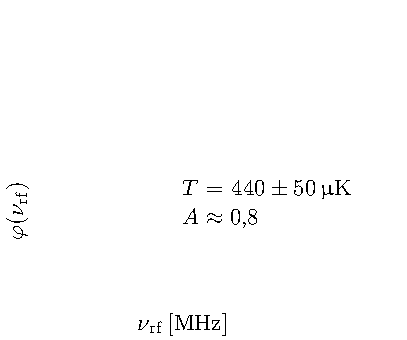
\includegraphics{P1/WithoutEvapFit}}
\begin{equation}
	\rapflux(\eta, \alpha) 
	 = 1 - A\,\left[ \val{1.7}\, \eta^{\val{1.1} - \val{0.4}\,\arctan(\val{3.6}\,\alpha)}
	\,\expo{-\val{0.9}\,\eta} \right] \nonumber
	\virguleformule
\label{eq:FitFunctionRapFlux}
\end{equation}
o� la variable $\nurf$ intervient dans la d�finition de $\eta$, et o� le param�tre ajustable $\Ttrans$ apparait dans les expressions de $\eta$ et $\alpha$ (voir les �quations~\nref{eq:alpha} et~\nref{eq:Eta}).
$A$ est un param�tre d�signant \emph{l'efficacit�} de l'antenne \rf utilis�e pour effectuer le filtrage. Nous tenons ainsi compte du fait que, sur les atomes devant �tre �limin�s par la zone de \firf, seule une fraction $A$ l'est effectivement.
%Rappelons que cette formule n'est utilisable que si l'on suppose que le \jat est � \eqthdy.
Dans la pratique, nous utilisons cette formule pour ajuster les deux param�tres inconnus $A$ et $\Ttrans$ sur les donn�es exp�rimentales d'un \spfirf. La figure ci-contre montre les donn�es de la figure~\nref{fig:SpectreEvap} ainsi que la fonction d'ajustement qui permet de d�terminer la temp�rature du jet. 
L'efficacit� d'une antenne est typiquement de $A = \val{80}\%$.

\RemarqueTitre{Pr�cision obtenue gr�ce � la formule approch�e}{
Une s�rie de simulations num�riques Monte-Carlo a montr� que cette formule approch�e permet de d�terminer la \tempt du \jat avec une erreur inf�rieure � $5\%$, et ce, pour une gamme de valeurs de $\alpha$ allant de $\val{0.1}$ � $\val{10}$. 
}

\subsubsection{Mise en \oe uvre exp�rimentale}
La figure~\nref{fig:MesureTempGuideImplementation} d�crit la mise en \oe uvre du protocole de mesure de la \tempt sur le \setup. 
%On y montre aussi une photographie d'une antenne \rf. 
Plus de d�tails techniques sont fournis dans la th�se de T.~Lahaye~\cite{TTL}.

\bfigh
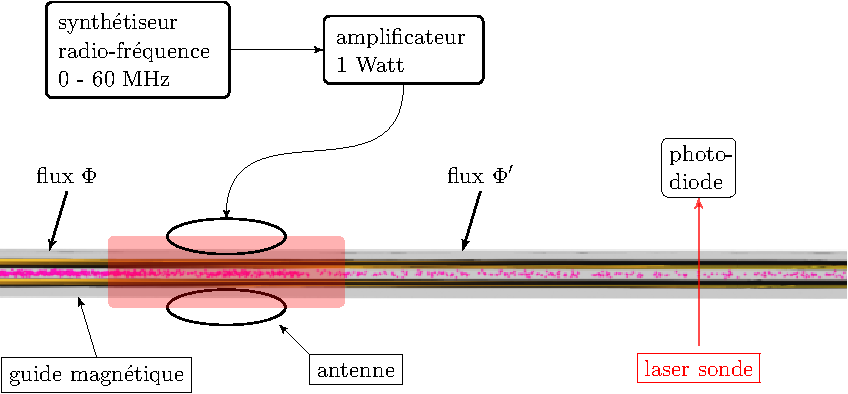
\includegraphics{P1/MesureTempGuideImplementation}
\CaptionFig{Mise en \oe uvre du protocole de mesure de la \tempt. Un synth�tiseur  fournit une \rf $\nurf$. Cette onde est alors amplifi�e jusqu'� une puissance de l'ordre du Watt. L'antenne dispos�e sur le \gm permet de diffuser localement l'onde sur les atomes pi�g�s. Il faut noter que la port�e de cette antenne au niveau du guide est d'environ \cm{20}(zone gris�e sur le sch�ma). En aval de l'antenne, \cad apr�s le filtrage, nous effectuons une mesure du \fat $\fluxapres$ par la technique d�crite dans la \autoref{sec:MesureDensiteGuide}. 
%\\ Comme dit pr�c�demment, la grandeur exp�rimentalement pertinente est le rapport $\rapflux = \ttfrac{\fluxapres}{\flux}$ des flux avant et apr�s la zone de filtrage. %Le \fat avant filtrage est mesur� tout simplement en stoppant l'�mission \rf. 
\\
Notons que le \sotosay{lieu physique} o� la \tempt du jet est mesur�e est donn� par la position de l'antenne \rf, et non par la position du laser sonde. En effet, c'est au niveau de l'antenne que se joue le processus de filtrage qui d�termine la fraction $\rapflux$ d'atomes qui atteindra le laser sonde.
}
\label{fig:MesureTempGuideImplementation}
\efigh

		\subsubsection{Limites de la m�thode}
	La m�thode spectroscopique de d�termination de la \tempt par \firf est tr�s fiable. Elle n'est toutefois pas utilisable dans tous les cas de figure. De mani�re � pouvoir l'appliquer, il faut notamment avoir � l'esprit les deux hypoth�ses importantes implicitement faites pour mener � bien le calcul de la fraction $\rapflux(\eta)$ d'atomes restant apr�s une zone de \firf:
	\begin{itemize}
	\item les \colels au sein du \jat sont n�glig�es pendant toute la travers�e de la zone de \firf,
	\item le r�le de la gravit� est n�glig�.
\end{itemize}	
On comprend bien le r�le de la premi�re hypoth�se: si elle n'est pas v�rifi�e, les collisions vont redistribuer les trajectoires atomiques \emph{pendant le filtrage}. En cons�quence, en plus d'�liminer les atomes v�rifiant le crit�re de filtrage, certains atomes \emph{ne v�rifiant initialement pas} ce crit�re, vont pouvoir changer de trajectoire et finalement �tre aussi �limin�s du jet.
\ApplicationNumerique
{Dans le cas de notre \jat, le \tcolel le plus �lev� obtenu est $\gammacol \approx \smun{5}$. La port�e $\Lantenne$ d'une antenne \rf est typiquement de \cm{20}. En consid�rant une vitesse du jet typique $\vjet = \cmps{60}$, le nombre de collisions durant la travers�e de la zone de filtrage est donc estim� par :
\[
 \frac{\gammacol \, \Lantenne}{\vjet} < 2 \mbox{ collisions}
 \pointformule
 \]
Dans ces conditions, des simulations num�riques Monte-Carlo ont montr� que cette technique de mesure de temp�rature reste tr�s fiable%
\footnotemark.
}
\footnotetext{Avec $\Ncol = 12$, la temp�rature est surestim�e de pr�s de $20\%$.}
La deuxi�me hypoth�se vise � simplifier la mod�lisation du probl�me. La force de gravit� rompt la sym�trie cylindrique du potentiel de pi�geage. Le moment cin�tique ne peut donc plus �tre consid�r� comme �tant une constante du mouvement. De plus, la surface du cylindre de filtrage ne correspond plus � une surface �quipotentielle. Cette hypoth�se est raisonnable dans le cas de notre configuration exp�rimentale (on se reportera � la th�se de T. Lahaye~\cite{TTL} pour plus de d�tails).
\ApplicationNumerique{
Comparons la force de gravit� � la force de rappel provenant du \gtchm. Il s'agit donc de comparer $m\,g$ � $\mu\gradB$. Dans le cas du \Rb dans le \snZ $\EtatFmF{1}{-1}$, l'�galit� de ces deux forces est obtenue pour un gradient:
\[
\gradB = \frac{m\,g}{\mu} \approx \gausspcm{30}
\pointformule
\]
Or, dans nos exp�riences, le \gtchm auquel sont soumis les atomes est plus d'un ordre de grandeur sup�rieur � cette valeur.
}




\section{�vaporation par cycles discrets et gain d'un facteur 10 dans l'\edpup}\label{sec:EvapRf}

Dans la section pr�c�dente, nous avons abord� le principe de la mesure de la \tempt du \jat par l'exploitation d'un \spfirf. 
%Fort de conna�tre la temp�rature du jet gr�ce � cette technique, il est alors 
Dans cette section nous allons montrer qu'il est possible d'utiliser le m�me principe de \fispse pour �liminer de mani�re contr�l�e certaines classes d'atomes du jet poss�dant une �nergie m�canique transverse �lev�e afin de modifier les caract�ristique du jet. C'est le principe mis en \oe uvre lors du \rpef d'un nuage atomique.% (voir la \autoref{sec:RefEvap}). 

Une �tude d�taill�e de l'\evap du \jat est men�e dans le chapitre 4 de la th�se de T. Lahaye~\cite{TTL} et je ne rappellerai donc ici que les r�sultats et concepts importants que j'ai eus � manipuler lors de mes deux premi�res ann�es de th�se.

\Resultat{
Afin d'�viter toute confusion, il est important pour la suite de distinguer le \firf utilis� dans les deux cas suivant:
\begin{itemize}
	\item le cas d�crit pr�c�demment de la mesure de \tempt qui exploite la mesure exp�rimentale d'un \spfirf. Cela consiste � \emph{mesurer les caract�ristiques} d'un \jat � l'\eqthdy. Cette mesure fait intervenir une antenne utilis�e � diff�rentes fr�quences $\nurf$, ainsi qu'un laser sonde pour mesurer les variations de flux $\rapflux(\nurf)$.
	\item le cas d�crit dans la suite de l'utilisation d'une zone de \firf dans le but pr�cis de \emph{modifier les caract�ristiques} du \jat par un processus d'\evap.% (voir la \autoref{sec:EvapForcee}).
\end{itemize}
Dans toute la suite, et sauf mention contraire, le \firf fera r�f�rence au deuxi�me cas.
}


\casse


\subsection{Rethermalisation du jet apr�s une zone de filtrage \rf}\label{sec:RethermJet}
%Jusqu'� pr�sent, nous nous sommes int�ress�s aux variations de \fat engendr�es par 
Le filtrage de certaines classes de trajectoires atomiques au sein du jet est synonyme d'une mise hors d'\eqthdy.	
L'�tude de la relaxation de ce jet \sotosay{filtr�} vers un nouvel �tat d'�quilibre a �t� expos� en d�tail dans les r�f�rences~\cite{TTL,LaG05}%, et nous n'en rappellerons donc que les r�sultats importants
.

Les pr�dictions th�oriques obtenues reposent simplement sur un bilan d'�nergie et de nombre de particules. 
%\Resultat
{
Les caract�ristiques du jet � l'\eqthdy avant le filtrage �tant donn�es par les cinq param�tres $(\vjet, \flux, T, \gradB, \alpha)$ et l'�nergie m�canique moyenne d'une particule �tant not�e $\Emoy$, le bilan est effectu� entre deux instants:
\begin{itemizel}
	\item tout de suite apr�s le filtrage spatial du jet, le flux de particules $\fluxapres$ ainsi que l'�nergie moyenne $\Emoyapres$, sont d�duits de la mani�re d�crite dans la \autoref{sec:MesureTempTrans},
	\item un temps arbitrairement long apr�s le filtrage, le jet �tant suppos� avoir atteint son nouvel �tat d'\eqthdy d�fini par $(\vjet, \fluxapres, T', \gradB, \alpha')$.
\end{itemizel} 
La conservation de l'�nergie et du nombre de particules pendant le processus de retour vers un nouvel �tat d'\eqthdy (gr�ce aux \colels) permet alors de d�duire la nouvelle temp�rature $T'$ du \jat.
}

Il n'existe pas de formulation analytique donnant $T'$ en fonction du param�tre de filtrage $\eta$ dans le cas d'un \cthyp%
%
%\footnote{Comme dans la section~\nref{sec:MesureTempTrans}, il existe une formule analytique dans le cas $\alpha \ll 1$, \cad quand les atomes sont confin�s dans un potentiel harmonique bi-dimensionnel. Pour plus de d�tails, on se reportera � la r�f�rence~\cite{TTL}%. La nouvelle temp�rature  d'\eqthdy est alors donn�e par \[ \left. \frac{T'}{T} \right|_{\alpha \ll 1} = 1 - \sqrt{\pi\,\eta}\,\Expo{-\eta}\].}%
.
\ifthenelse{\FormatEUE > 0}{}
{\AjouteLigne}
En pratique, une int�gration num�rique est utilis�e pour pouvoir pr�dire le comportement du \jat. Nous montrons dans la figure~\nref{fig:TsurTGuide} la courbe donnant la variation de temp�rature $\tfrac{T'}{T}$ en fonction du param�tre de filtrage $\eta$ dans les deux cas asymptotiques $\alpha \gg 1$ (correspondant � un \pthar) et $\alpha \ll 1$ (correspondant � un \ptlin).
\bfighs
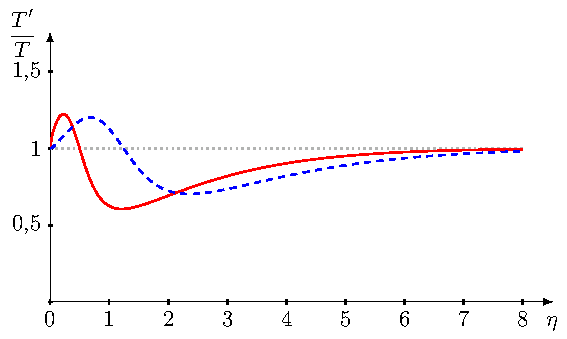
\includegraphics{P1/TsurTGuide}
\RemonteUnPeuFig\RemonteUnPeuFig
\CaptionTocCaptionFig{Variations relatives de la temp�rature du jet apr�s une zone de \firf}{Variations relatives $\ttfrac{T'}{T}$ de la temp�rature du jet apr�s une zone de \firf de param�tre $\eta$, et une \reth compl�te. La courbe est repr�sent�e dans les deux cas limites d'un \cthar, $\alpha \gg 1$ (trait plein), et d'un \ctlin $\alpha \ll 1$ (trait tiret�). Il est possible de refroidir le \jat si $\eta$ est sup�rieur � une valeur limite $\etalim$. Le comportement asymptotique de ces courbes est bien compris:\\
\vtop{\linewidth=\CaptionWidth %
\begin{itemize}
\item pour $\eta \gg \etalim$, les atomes �limin�s du jet poss�dent une grande �nergie m�canique, sup�rieure � l'�nergie moyenne $\Emoy$. L'�nergie moyenne par atome $\Emoyapres$ apr�s le filtrage est donc plus faible. La nouvelle temp�rature d'�quilibre est plus faible,  $\ttfrac{T'}{T} \lesssim 1$.
\item pour $\eta \ll \etalim$ les atomes �limin�s poss�dent globalement une �nergie m�canique inf�rieure � l'�nergie moyenne. L'�nergie moyenne par atome augmente donc. La nouvelle temp�rature d'�quilibre est plus �lev�e, $\ttfrac{T'}{T} \gtrsim 1$.
\item par ailleurs, si le rayon du cylindre de filtrage est nul ($\eta \rightarrow 0$), ou infini ($\eta \rightarrow \infty$), aucun atome n'est �limin�, et la temp�rature reste inchang�e, $\ttfrac{T'}{T} = 1$.
\end{itemize}
}
}
\label{fig:TsurTGuide}
\efigh

\pagebreak

\noindent
Sur la figure~\nref{fig:TsurTGuide}, on constate qu'il est possible de refroidir le jet si $\eta$ est pris suffisamment grand: 
\begin{itemizel}
	\item $\eta > \val{0.5}$ pour un pi�geage transverse harmonique.
	\item $\eta > \val{1.18}$ pour un pi�geage transverse lin�aire.
\end{itemizel}

\EnFaitNon{\nRemarque{Le fait qu'il soit aussi possible de chauffer le jet peut para�tre surprenant de prime abord \dixit{si l'on se repr�sente, � tort, le processus d'\evap comme l'�limination des particules les plus �nerg�tiques. En effet, nous avons vu page \pageref{Rq:CritereFiltrage} que le crit�re de filtrage porte non pas sur l'�nergie d'un atome, mais sur le couple (�nergie, moment cin�tique). La figure \vref{fig:TrajGuide} montre d'ailleurs que certains atomes tr�s �nerg�tiques sont conserv� lors de la phase de filtrage.}
}
}

\noindent \dixit{Nous devons maintenant nous demander comment varient les deux param�tres cruciaux du jet:
\begin{itemizel}
	\item la \ddedpup $\rhojetaxe$ sur l'axe $z$,% que l'on veut augmenter le plus possible, 
	\item le \tcolel $\gammacol$.% qui doit rester important, voire augmenter. C'est en effet ce param�tre qui d�termine la cin�tique du retour � l'�quilibre\footnote{Si $\gammacol$ devient tr�s faible, cela veut tout simplement dire que le refroidissement (au sens d'atteindre un nouvel �tat d'\eqthdy) ne se fait qu'au bout d'un temps extr�mement long.}.
\end{itemizel}
}

La figure \vref{fig:RhoGammaGuide} repr�sente les variations attendues $\ttfrac{\rhojetaxeapres}{\rhojetaxe}$ et $\ttfrac{\gammacolapres}{\gammacol}$ de ces deux grandeurs, dans les deux cas limites $\alpha \gg 1$ et $\alpha \ll 1$.
\bfigsss
\subfloat[]{\label{fig:RhosurRhoGuide}
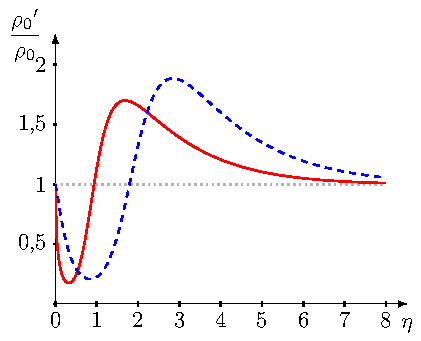
\includegraphics{P1/RhosurRhoGuide}}
\subfloat[]{\label{fig:GammasurGammaGuide}
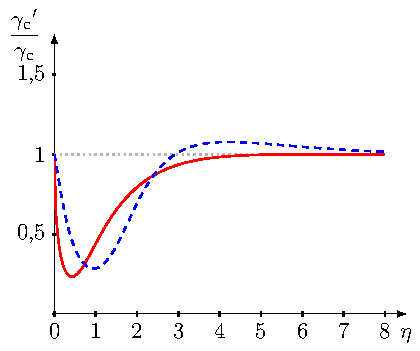
\includegraphics{P1/GammasurGammaGuide}}
\CaptionFigs{Courbes repr�sentant les variations relatives (a) de la \ddedpup $\ttfrac{\rhojetaxeapres}{\rhojetaxe}$ sur l'axe $z$ ; (b) du \tcolel $\ttfrac{\gammacolapres}{\gammacol}$ \emph{apr�s une zone de \firf} de param�tre $\eta$, et une \reth compl�te. Sont envisag�s ici les deux cas limites d'un \cthar, $\alpha \gg 1$ (trait plein), et d'un \ctlin $\alpha \ll 1$ (trait tiret�).
}
\label{fig:RhoGammaGuide}
\efig

\noindent Cette figure montre notamment que la \ddedpup augmente si $\eta$ est choisi suffisamment grand. En revanche, on constate que le \tcolel ne peux pas �tre augment� dans le cas d'un \cthar%
%
\footnote{En toute rigueur, il est th�oriquement possible dans un \cthar et pour $\eta \approx 7$, d'augmenter le \tcolel d'environ $\val{0.1}\%$. Ce qui n'est en pratique absolument pas exploitable.}%
. 
Le \ctlin semble �tre plus profitable du point de vue du processus d'\evap. En effet: 
\begin{itemize}
	\item  le gain relatif en \ddedpup peut alors atteindre $\val{1.9}$ contre $\val{1.7}$ pour un pi�geage harmonique,
	\item ce gain maximum est obtenu pour un param�tre $\eta \approx \val{2.9}$ qui, sur le plan du \tcolel, correspond � une augmentation sensible de quelques pour cent. Le pi�geage harmonique implique une diminution d'environ $25\%$ du \tcolel si l'on d�sire obtenir le gain maximal de $\val{1.7}$ en \ddedp%
	%
\footnote{Dans ces conditions, l'enchainement de 5 zones d'�vaporation conduirait th�oriquement � une r�duction du \tcolel par facteur \val{1000}.}.
\end{itemize}

\Remarque{
L'impossibilit� d'augmenter le \tcolel $\gammacol$ dans le cas du potentiel harmonique est propre au caract�re \bd du confinement~\cite{LaG06,DMK95}. 
Il est tout � fait possible d'augmenter le $\gammacol$ dans un pi�ge harmonique \td (tel qu'un pi�ge de \IP). 
Cette limite est un lourd handicap puisqu'elle interdit l'\termetech{emballement} du processus d'�vaporation%
%\footnote{L'\termetech{emballement} traduit l'augmentation du \tcolel au fur et � mesure de l'�vaporation, qui permet}%
.
% telle qu'elle est d�crite dans la \autoref{sec:EvapForcee}. 

L'utilisation d'un potentiel \tlin ($\alpha \ll 1$) semble donc souhaitable. Cependant, le param�tre $\alpha$ est d�termin� par la temp�rature du jet. En atteignant des temp�ratures de plus en plus faibles, on finira toujours par avoir $\alpha > 1$.
}


\RemonteUnPeuFig
\RemonteUnPeuFig

\subsection{Gain d'un facteur 10 dans l'\edpup}\label{sec:Gain10}
\noindent \dixit{Dans la sous-section pr�c�dente, la dynamique du retour � l'\eqthdy via les \colels entre atomes a �t� compl�tement pass�e sous silence. Or, il s'agit d'un point crucial dans la perspective d'un refroidissement pouss� du jet.
} 
Le temps n�cessaire au jet pour effectuer son retour � un \eqthdy se formule en termes de nombre moyen $\Ncol$ de \colels entre atomes. Pour plus d'information, on consultera avec int�r�t les r�f�rences~\cite{LaG05,LaG06}%
%
\footnote{Un point remarquable est d�taill� ces deux articles. Celui-ci a initialement �t� mis en �vidence dans la r�f�rence~\cite{AnG06}: la dynamique du retour � l'\eqthdy d�pend de mani�re notable de la g�om�trie du potentiel. Ainsi, dans un \pptlin, un jet mis hors d'�quilibre par une zone de \firf va demander, pour \rether, jusqu'� $2$ fois plus de \colels que dans le cas d'un \cthar.}. 

%Nous avons mentionn� pr�c�demment qu'u
Une mani�re d'augmenter le nombre de \colels au sein du \jat est de mettre en place une \secpent dans le \gm. Sur notre \setup, on atteint gr�ce � ce proc�d� $\Ncol = 20$. 
\dixit{L'utilisation de plusieurs zones d'�vaporation est alors envisageable, dans le but d'obtenir un gain significatif en \ddedp.} 

%\ifthenelse{\FormatEUE > 0}{}
{\AjouteLigne}

\RemonteUnPeuFig
\RemonteUnPeuFig

\subsubsection{Dispositif � 11 zones d'�vaporation}
\noindent Sur notre \setup, 11 zones d'�vaporation ont �t� plac�es le long du \gm (voir la figure~\nref{fig:Montage10Antennes}). 
Elles sont r�parties tout les \cm{20}, sauf sur la section centrale o� les �l�ments de connexion en acier emp�chent les ondes \rf d'atteindre le jet.
%
\RemonteUnPeuFig
\RemonteUnPeuFig
\bfighss
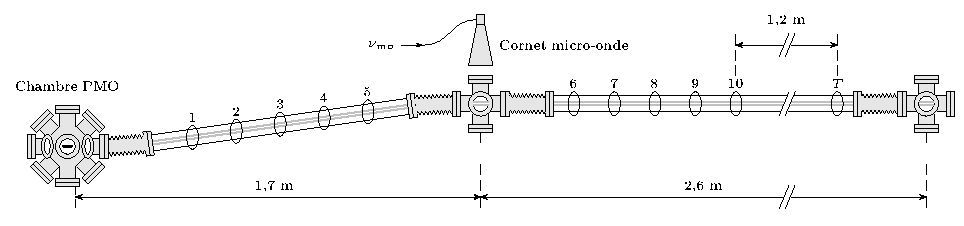
\includegraphics[width=\FigWidth]{P1/Montage10Antennes}
\CaptionFigssss{Disposition des antennes \rf (repr�sent�es par des ellipses num�rot�es de 1 � 10) et du cornet micro-onde utilis�s pour produire l'enchainement de zones d'�vaporation du \jat.
Des connexions en acier permettent de joindre les deux sections du tube de verre entourant le guide. Seules les micro-ondes permettent une �vaporation efficace du jet dans cette zone. 
Notons qu'une distance de \m{1.2} � la fin du guide est d�pourvue de zone d'�vaporation afin de permettre le retour � l'\eqthdy du jet avant d'effectuer la mesure du \spfi qui d�termine la temp�rature (antenne not�e $T$).
}
\label{fig:Montage10Antennes}
\efigh
%

\casse

\nRemarqueTitre{Utilisation d'une antenne micro-onde}{
	Nous avons mis en \oe uvre une technique d'�vaporation \emph{micro-onde} sur notre \setup. Celle-ci repose sur le \fisp identique � celui d�crit dans la \autoref{sec:RethermJet}, mais en utilisant des transitions entre \snhfs.
Pour plus de d�tails, on pourra se reporter � la th�se de T.~Lahaye~\cite{TTL}. Mentionnons toutefois les deux avantages de cette technique :
\begin{itemize}
	\item trois transitions, $\EtatFmF{1}{-1}\longrightarrow\EtatFmF{2}{0,1,2}$, sont autoris�es. Chacune d'elle correspond, pour une fr�quence $\numo$ donn�e, � trois rayons de cylindre de filtrage diff�rents. L'�vaporation en est rendue plus efficace.
	\item les micro-ondes (� la diff�rence des ondes \rf) se propagent bien � l'int�rieur des tubes de connexion en acier qui compose le syst�me � \uv. On peut donc utiliser cette technique pour effectuer l'�vaporation � l'int�rieur d'une chambre � vide m�tallique en pla�ant le cornet �metteur devant un hublot. Dans le cas plus sp�cifique du \jatgm, nous pouvons cr�er une zone de filtrage entre les deux sections du guide (voir la figure~\nref{fig:Montage10Antennes}).
\end{itemize}
}

\ifthenelse{\FormatEUE > 0}{}
{\AjouteLigne}
	
	\subsubsection{Gain en \ddedp}
La figure~\nref{fig:Gain10Spectre} montre les \spfirfs mesur�s gr�ce � la derni�re antenne (not�e $T$ sur la figure~\nref{fig:Montage10Antennes})  dans les deux cas suivant:
\begin{itemize}
	\item le \jat non refroidi, \cad sans les antennes d'�vaporation,
	\item le m�me jet, mais apr�s son passage dans la succession des 11 zones d'�vaporation.
\end{itemize}
%
\bfighs
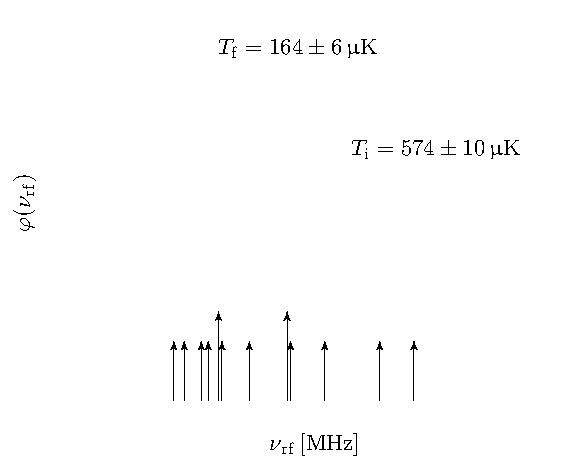
\includegraphics{P1/Gain10Spectre}
\CaptionFigss{Spectre de \firf permettant de d�terminer les caract�ristiques du \jatgm dans les deux cas du jet non-refroidi (\cad sans les antennes d'�vaporation repr�sent�es sur la figure~\nref{fig:Montage10Antennes}) et du m�me jet mais ayant travers� les 11 zones d'�vaporation. Les fl�ches repr�sentent les \rfs utilis�es par les antennes. 
Les fl�ches plus longues correspondent � la zone d'�vaporation micro-onde, en termes de \rfs qui donneraient les m�me rayons d'�vaporation.\newline
Le \spfirf initial correspond � une temp�rature $\Tini = \microKpm{574}{10}$. Apr�s retour � l'\eqthdy le \spfi est beaucoup moins large, traduisant le fait que la temp�rature est plus faible: $\Tfin = \microKpm{164}{6}$}
\label{fig:Gain10Spectre}
\efigh
\Cahier{6,166}

\Resultat%
{
\noindent
Les donn�es exp�rimentales repr�sent�es sur la figure~\nref{fig:Gain10Spectre}, ainsi qu'une mesure du \fat permettent d'effectuer le bilan dans l'encadr� ci-dessous:
\vspace{1ex}
\begin{center}
%\begin{Large}
\begin{tabular}{|lcccl|}
\hline
  Jet non �vapor�   &    & &  &  Jet �vapor�   %\vspace{3ex} 
\\
$\vjet = \cmps{60}$  &    &  &  &  $\vjet = \cmps{60}$    %\vspace{1.5ex}
\\
$\flux \approx \atps{7E{9}}$ &  &\huge{${\Longrightarrow}$} & & $\fluxapres \approx \atps{9E{8}}$     %\vspace{1.5ex}
\\
$T = \microKpm{574}{10}$ & & & & $T' = \microKpm{164}{6}$   \vspace{-2.5ex} %\vspace{1.5ex}
\\
$\underbrace{\phantom{T = \microKpm{574}{10}}}_{}$  &  &  &    & $\underbrace{\phantom{T' = \microKpm{164}{6}}}_{}$  \vspace{-1ex}
\\
$\rhojetaxe \approx \val{2.0E{-8}}$ & & & & $\rhojetaxe \approx\val{2.1E{-7}}$\\ %\vspace{1.5ex}
\hline
\end{tabular}	
%\end{Large}
\end{center}
\vspace{1ex}
Nous d�montrons ainsi un gain en \ddedpup d'un facteur $\val{10.4}^\val{+4.1}_\val{-3.0}$. 
%Ce r�sultat fait l'objet de la r�f�rence~\cite{LWR05}. 
}

\section{Conclusion}
	\subsection{Difficult�s inh�rentes � l'\evap d'un \jatg}\label{sec:DifficultesInherentes}
On peut s'interroger sur le fait qu'il semble difficile d'obtenir un gain sur $\rhojetaxe$ sup�rieur � 1 ordre de grandeur. En effet l'utilisation du \rpef sur une exp�rience typique de \condbe permet de gagner plusieurs ordres de grandeur en \ddedpup.

Notons tout d'abord que la succession des 11 zones d'�vaporation dont il est question plus haut conduirait th�oriquement � un gain \val{1600} sur $\rhojetaxe$, si l'on supposait une \reth compl�te du jet entre chaque zone. En r�alit�, le nombre $\Ncol \approx 20$ de \colels au sein du jet ne permet pas d'obtenir ce gain. 

\Resultat
{\label{JetAtomiqueDifficultees}
Soulignons les trois raisons principales qui font que l'\evap d'un \jat est une t�che fondamentalement plus ardue que pour un nuage d'atomes pi�g�s:

\begin{itemize}
	\item le simple fait de produire un \j � partir de l'injection puls�e de \pats implique une \emph{dilution spatiale} des \ps suivant l'axe du \gm. Ceci se traduit par une perte en \dat, et donc en \tcolel%
%	\footnotemark.
	\item le guide ayant une longueur finie, le temps allou� pour r�aliser l'�vaporation est limit� par le \emph{temps de propagation}. En pratique nous disposons d'environ \seconde{6}.
	\item le \emph{confinement purement transverse} rend le processus d'�vaporation moins efficace que dans le cas d'un pi�geage \td%
	\footnotemark.
\end{itemize}
}
%\footnotetext{La perte en \tcolel d� � la dilution spatiale des \ps est estim�e � un facteur $6$.}
\footnotetext{Comme nous l'avons soulign�, il est en particulier impossible d'observer un emballement de l'�vaporation dans un \ppthar.}

\subsection{N�cessit� de d�velopper de nouveaux outils}

Dans ce chapitre nous avons d�crit le \setup qui nous a permis de mettre en \oe uvre le \rpef d'un \jatuf \mg. Le gain d'un facteur $10$ sur la \ddedp semble faible face aux sept ordres de grandeur qui nous s�parent encore de la \condbe. Le param�tre physique qui nous limite est en fait le nombre moyen $\Ncol$ de collisions subies par un atome au cours de sa propagation. Une estimation montre que si nous pouvions disposer d'un nombre dix fois plus �lev� de collisions (soit $\Ncol\approx200$), le \rdq serait alors accessible. La figure~\nref{fig:EvolutionNC} montre l'�volution du nombre de collisions $\Ncol$ lors des diff�rentes �volutions du \setup.
\bfig
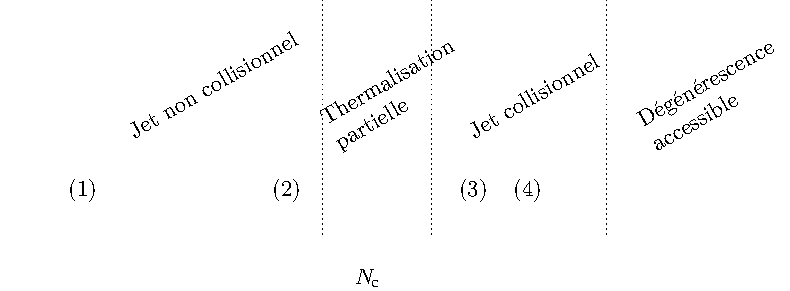
\includegraphics{P1/EvolutionNC}
\CaptionFig{Repr�sentation de l'�volution du nombre de \colels $\Ncol$ subies en moyenne par chaque atome au cours de sa propagation le long du \gm. Les diff�rentes �tapes chronologique, dans le cadre de notre exp�rience, sont repr�sent�e par des points: (1) en 2002~\cite{CRA02}, (2) en 2003~\cite{RCL03}, (3) en 2004~\cite{LVG04}, (4) en 2005~\cite{LWR05}.
}
\label{fig:EvolutionNC}
\efig

\noindent La plupart des chapitres de ce manuscrit de th�se sont d�di�s � l'�tude de diff�rentes possibilit�s visant � contrecarrer les trois difficult�s mentionn�es dans l'encadr� \vpageref[ci-dessus ][de la ]{sec:DifficultesInherentes} :
\begin{itemize}
	\item le chapitre~\nref{chap:MiroirMobile} pr�sente une nouvelle m�thode de ralentissement des \ps inject�s dans le guide gr�ce � l'utilisation d'un \mimamo. Nous montrerons en particulier que cette m�thode, contrairement � l'utilisation d'une \secpent, peut th�oriquement \emph{augmenter} la \ddedpup du jet obtenu par recouvrement des \ps.
	\item le chapitre~\nref{chap:Convoyeur} traite du transport des \pats dans un train de pi�ges de Ioffe-Pritchard. Le fait de pr�server momentan�ment (sur le premier m�tre du guide) un pi�geage \td permet de conserver un \tcolel �lev� et de rendre l'�vaporation plus efficace.
	\item le chapitre~\nref{chap:PiegeDipolaire} consiste en l'�tude de la production de \ps tr�s denses dans un pi�ge dipolaire. En augmentant le \tcolel ainsi que la \ddedp des \pats, nous pouvons esp�rer produire un \jatuf dont les caract�ristiques initiales seraient plus favorables pour mener � bien le \rpef.
\end{itemize}

\chapter{\TitreChapitreDeux}\label{chap:Ceramique}

\bfigh
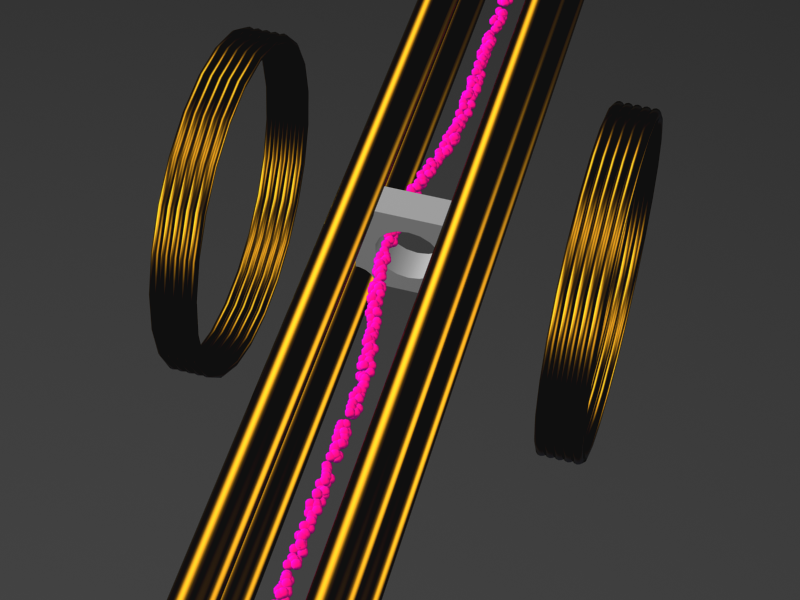
\includegraphics[width=\FigWidth]{P1/ChapitreCeramique}
\SansCaption
\efigh

\pagebreak

\minitoc
\vspace{0.5cm}
 
Dans le chapitre précédent, nous avons décrit le \setup qui nous permet d'effectuer l'\evap d'un \jatgm. Rappelons que le \fispse des atomes énergétiques y est mené à bien par la mise en place d'antennes radio-fréquences et micro-ondes le long du \gm. Cette technique usuelle d'évaporation souffre cependant d'un défaut majeur : si l'efficacité du filtrage est d'autant plus grande que la puissance de l'onde électromagnétique est élevée, la portée de l'antenne augmente alors également. Celle-ci est d'environ \cm{20} pour une antenne \rf utilisée dans les conditions expérimentales décrites dans la \autoref{sec:Gain10}. 

Dans la perspective d'utiliser un grand nombre de zones d'évaporation, il est primordial de pouvoir disposer d'une technique de \fisp \emph{efficace} et d'action \emph{très locale}. 
Dans ce chapitre, nous présentons une méthode qui répond à ces deux critères. Elle consiste en l'élimination sélective d'atomes par adsorption sur une surface diélectrique. 


\section{Mise en \oe uvre}\label{sec:EvapCeramMiseEnOeuvre}
L'évaporation par élimination d'atomes au contact d'une surface matérielle a été démontrée pour la première fois en 2003 par le groupe d'Eric Cornell~\cite{HMO03}. Ces travaux  montrent en outre que le caractère isolant (diélectrique) du matériau utilisé joue un rôle primordial : d'importantes pertes d'atomes sont observées lorsqu'un nuage magnétiquement piégé est approché à quelques dizaines de microns de la surface d'un conducteur%
\footnote{La raison en est que les fluctuations thermiques de courant à l'échelle microscopique d'un conducteur sont suffisantes pour induire de fortes fluctuations de \chm au voisinage de sa surface. Ces fluctuations peuvent alors provoquer des transitions entre \snZ vers des états non-piégés~\cite{HMO03,LTC04}.}%
.

\casse

Pour une surface en cuivre, excellent conducteur, les pertes commencent à se faire ressentir à une distance d'environ $\micron{200}$. 
En revanche, l'utilisation d'une surface de silicium permet de d'éliminer selectivement les atomes par contact avec la surface afin de mener à bien l'évaporation, éventuellement jusqu'au \rdq~\cite{LTC04}.


Cette section expose le principe de cette technique, ainsi que sa mise en \oe uvre sur notre \setup, \cad transposée au cas d'un \jatgm.


\subsection{Principe de la méthode}
Cette sous-section expose le principe de la méthode d'élimination d'atomes au contact d'une surface. Cette technique consiste en un \fispse d'atomes piégés par un champ de forces conservatives. 
Elle consiste 
%, comme dans le cas de l'évaporation par \firf, 
à éliminer les atomes dont l'énergie mécanique est élevée et sont la trajectoire atteint la surface d'un solide placé à proximité du piège. Au contact de celle-ci, les atomes sont éliminés%
\footnote
{
On peut raisonnablement considérer deux processus expliquant pourquoi l'atome qui entre en contact avec la surface est éliminé du piège:
\begin{itemize}
	\item l'adsorption, \cad que l'atome reste \sotosay{collé} à la surface et ne revient plus dans le piège.
	\item la surface étant à température ambiante ($\approx\SI{300}{\kelvin}$), l'agitation thermique de celle-ci peut communiquer une énergie cinétique considérable à toute particule qui  entre en contact avec elle. L'atome est alors \sotosay{éjecté} du piège.
\end{itemize}
}
du piège (voir la figure~\nref{fig:CeramPrincipe}).
\bfigh
\RemonteUnPeuFig
\subfloat[]
{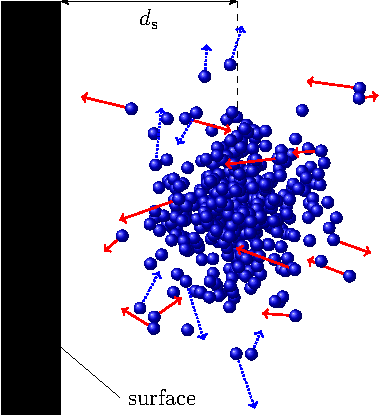
\includegraphics{P1/CeramPrincipe_a}} \qquad \qquad \qquad
\subfloat[]
{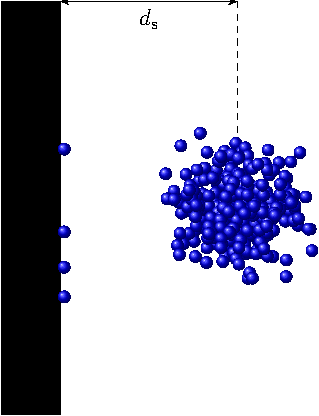
\includegraphics{P1/CeramPrincipe_b}}
\CaptionFigss{Principe de l'élimination sélective d'atomes sur une surface matérielle. \\
(a) : Un piège atomique est approché à une distance $\CeramDist$ d'une surface matérielle. Certains atomes (ceux dont le vecteur vitesse a été représenté) possèdent assez d'énergie mécanique pour atteindre la surface. Cependant, certains de ces atomes (dont le vecteur vitesse est représenté en pointillé) n'atteindrons pas la surface du fait de l'orientation de leur trajectoire. Ce mode d'évaporation est a priori unidimensionnel, \cad qu'il n'agit que sur un degré de liberté. \\
(b) : au contact de la surface, les atomes ont été éliminés du piège. Via les \colels entre atomes restants, le système évoluent vers un nouvel état d'\eqthdy d'énergie moyenne plus faible. Pour poursuivre l'évaporation, on peut alors diminuer à nouveau la distance $\CeramDist$.
}
\label{fig:CeramPrincipe}
\efigh

\subsection{Adaptation de la technique à un \jmg}
Afin d'adapter cette technique à un \jmg, il nous faut dévier la trajectoire de ce dernier vers une surface diélectrique placée dans le système à \uv. Notre \setup n'ayant initialement pas été prévu pour cette tâche, nous avons mis à profit les pièces de céramique qui servent à maintenir les tube de notre \gm (voir la figure~\nref{fig:CeramGuide}). 
\bfigh
\RemonteUnPeuFig
\subfloat[]
{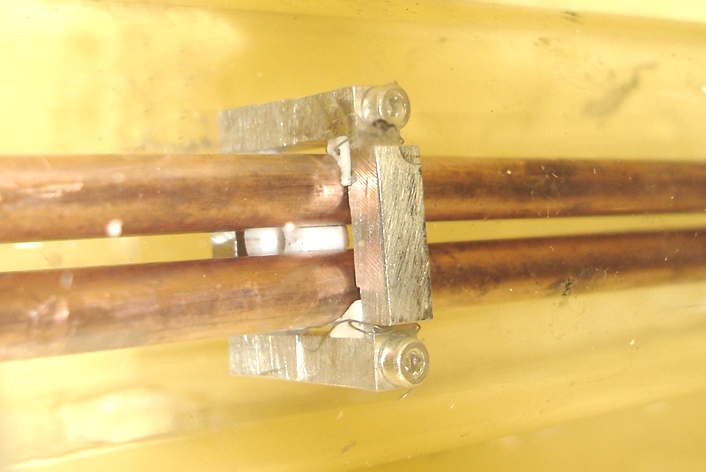
\includegraphics[height=6cm]{P1/DSC03881_Modif}}
\subfloat[]
{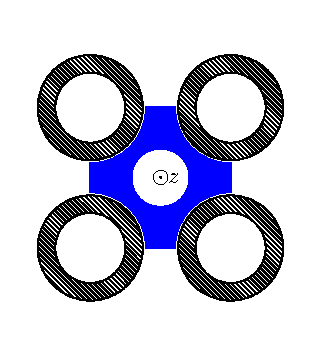
\includegraphics{P1/CeramTubes}} 

\RemonteUnPeuFig
\subfloat[]
{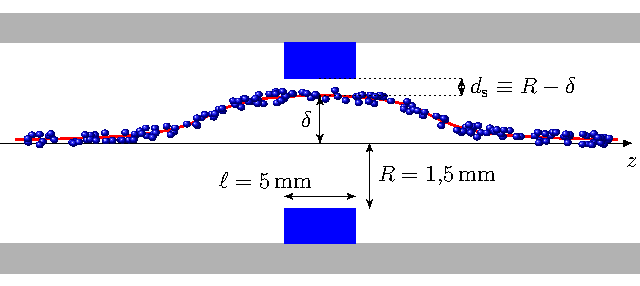
\includegraphics{P1/CeramTubesVueHaut}\label{fig:CeramGuide_c}}
\CaptionFig{Afin de maintenir les quatre tubes de cuivre à une distance donnée les uns des autres, des pièces de céramique sont réparties environ tous les \cm{40} le long du guide. La photographie (a) représente l'une de ces pièces à l'intérieur du tube de verre dans lequel règne un vide poussé. Le schéma (b) représente une coupe à l'échelle $3$ du guide au niveau d'une pièce de céramique (dessinée en bleu). La longueur d'une céramique est $\CeramLong=\mm{5}$. Le trou central de rayon $\CeramRay=\mm{1,5}$ permet au \jat de se propager suivant l'axe $z$ du guide. Le schéma (c) montre, vu de dessus, le jet localement dévié d'une distance $\Devi$ hors de cet axe. Si cette déviation se fait lors du passage dans l'une des céramiques, des atomes suffisamment énergétiques du jet peuvent être éliminés.}
\label{fig:CeramGuide}
\efigh

\ifthenelse{\FormatEUE > 0}{}
{\AjouteLigne}

Les \pdecs sont réparties environ tous les \cm{40} tout au long du guide et comportent un trou central de rayon $\CeramRay=\mm{1,5}$ %
\nome{\CeramRay}{Rayon du trou central des \pdecs}%
 au centre duquel passe le jet d'atome froids. L'extension longitudinale (selon l'axe $z$) de ces pièces est de $\CeramLong=\mm{5}$%
\nome{\CeramLong}{Extension longitudinale (selon l'axe $z$) des \pdecs}.
Il s'agit alors de dévier la trajectoire du jet d'une distance $\Devi$%
\nome{\Devi}{Déviation de la trajectoire du jet hors de l'axe $z$ du guide}%
 hors de l'axe $z$ vers le bord de l'une de ces \pdecs (voir la figure~\nref{fig:CeramGuide_c}). 


\subsubsection{Rappel sur le \gm}
Avant toute chose, rappelons que les quatre tubes de cuivre du guide produisent une configuration \qp de \chm.
Celle-ci se caractérise par une valeur minimale du champ tout au long de l'axe $z$ du guide. C'est autour de cette ligne que les atomes piégés dans l'état $\EtatFmF{1}{-1}$ orbitent durant leur propagation. 
Rappelons ici l'expression du vecteur \chm produit au voisinage de l'axe $z$ du guide (voir \vpageref{sec:ConfigMagnetiqueGuide}):
\[
	\vectBxyz = \vVecteur{-\gradB\,x}{\gradB\,y}{\Bpara} \mbox{\qquad avec \qquad} \gradB \equiv \frac{4\,\mu_0}{\pi\,\espTubes^2}\,I 
	\virguleformule
%	\label{eq:BQuadrAgain}
\]
où $\gradB\approx\gausspcm{800}$ est le \gtchm produit par le guide et $\Bpara\approx\gauss{1}$ est le champ uniforme longitudinal que nous ajoutons afin de minimiser les pertes par retournement de spin (voir \vpageref{AN:ValeurB0}).
\Remarque{
Dans tout ce chapitre, la température typique du \jat est de l'ordre de \microK{600}. Dans ces conditions, et comme nous l'avons vu dans la \autoref{sec:ConfigMagnetiqueGuide}, le \ppt \sotosay{ressenti} par les atomes est alors essentiellement linéaire (le paramètre $\alpha$ vaut environ $0,05$).%qui permet de mesurer l'harmonicité apparente du
}
La figure~\nref{fig:GuideChampTransverse_a} représente quelques lignes de champ dans un plan $(x,y)$, perpendiculaire à l'axe du guide. La figure~\nref{fig:GuideChampTransverse_b} montre, quant à elle, quelques vecteurs champs dans le plan horizontal $(x,z)$ contenant l'axe $z$ du guide. 
\bfigh
\subfloat[]
{\label{fig:GuideChampTransverse_a}
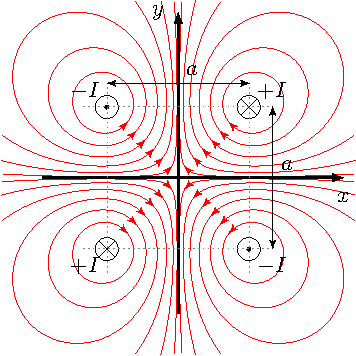
\includegraphics{P1/TubesQuadrupole_a}
}
\subfloat[]
{\label{fig:GuideChampTransverse_b}
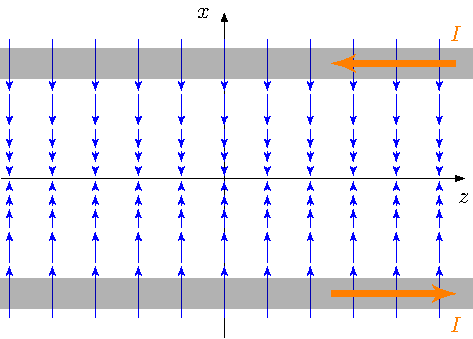
\includegraphics{P1/TubesQuadrupole_XZ}
}
\CaptionFig{Configuration de \chm \qpdd. (a): représentation de quelques lignes de champ dans le plan transverse $(x,y)$. (b) : dessin de quelques vecteurs champs dans une vue de dessus contenant l'axe du guide (l'unité de longueur des vecteurs est arbitraire). Le champ converge vers l'axe $z$ dans le plan $(x,z)$, et il diverge dans le plan vertical $(y,z)$. 
La position des tubes de cuivre est représentée par des zones grisées.}
\label{fig:GuideChampTransverse}
\efigh

\pagebreak

\subsection{Déviation du jet à l'aide d'une paire de bobines}\label{sec:EvapCeramBobines}
%Si nous pouvons utiliser l'une des \pdecs afin d'éliminer des atomes du jet, il nous faut encore disposer d'un moyen de dévier la trajectoire de ce dernier. 
Cette sous-section décrit l'une des deux méthodes que nous avons utilisées afin de dévier la trajectoire du jet. L'autre méthode (faisant intervenir des aimants permanents) fait l'objet de la \autoref{sec:EvapCeramAimants} en fin de ce chapitre.

Pour décaler la ligne qui correspond, à un minimum de module du \chm, il suffit de superposer localement un champ $\CeramBtrans$ %
\nome{\CeramBtrans}{Champ magnétique transverse permettant de dévier la trajectoire du jet}%
suivant une direction perpendiculaire à l'axe $z$. Dans notre cas, la direction du champ $\CeramBtrans$ est prise suivant l'axe $x$ de manière à dévier la trajectoire dans un plan horizontal%
%\footnote{De cette manière, nous évitons et à s'affranchir ainsi de variations d'altitude}%
.
L'amplitude $\Devi$ de la déviation hors de l'axe $z$ est alors donnée par :
\begin{equation}
	\Devi = \frac{\CeramBtrans}{\gradB}
\pointformule
\label{eq:Devi}
\end{equation}
Il faut cependant veiller à ne pas moduler la composante longitudinale du \chm (selon l'axe du guide). Nous verrons en effet dans le chapitre~\nref{chap:MiroirMobile} que cela aurait pour effet de produire une \bapot le long de l'axe du guide. 

Nous utilisons deux bobines de rayon \cm{4,5} et réalisées avec 107 tours de fil de cuivre de \mm{1,8} de diamètre. Comme le montre la figure~\nref{fig:GuideChampTransBobines}, elle sont placées symétriquement de part et d'autre du guide, à \cm{5} de l'axe $z$%
%\footnote{Les bobines  tube de verre dans lequel règne l'\uv ayant un }%
 et sont parcourues \emph{dans le même sens} par un courant ajustable de $0$ à \SI{40}{\ampere}. 
\bfigh
\subfloat[]
{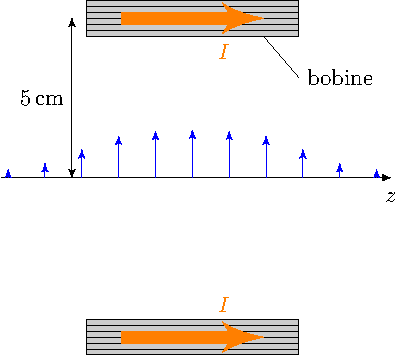
\includegraphics{P1/GuideChampTransBobines_a}
}
\subfloat[]
{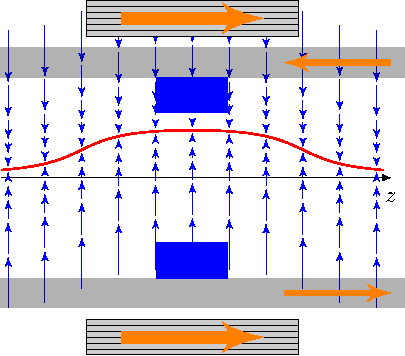
\includegraphics{P1/GuideChampTransBobines_b}
}
\CaptionFig{Représentation de l'effet de la superposition d'un \chm transverse sur le champ du guide.
(a) : dessins de quelques vecteurs champ pris le long de l'axe $z$, en ne considérant que les bobines positionnée symétriquement autour de l'axe du guide. 
(b) : représentation schématique de quelques vecteurs \chm lorsqu'on superpose le champ des bobines à celui du \gm. La ligne correspondant à un minimum local de \chm est déviée de l'axe $z$.}
\label{fig:GuideChampTransBobines}
\efigh

La configuration à deux bobines (qui rappelle une configuration Helmholtz) est parfaitement adaptée à nos besoins puisque le champ produit est purement transverse%
\footnote{Le champ est purement transverse sur l'axe $z$, mais ceci n'est plus vrai le long de la trajectoire moyenne des atomes qui est précisément déviée en dehors de cet axe. Cet effet est cependant complètement négligeable pour les extensions transverses considérées (voir l'application numérique).}
en tout point de l'axe $z$ du \gm. 
%De plus, le module du champ est quasiment constant au voisinage de la céramique. Ainsi le confinement transverse autour de la position d'équilibre n'est pratiquement pas modifié. 
\ApplicationNumerique{
Pour toutes les expériences décrites dans ce chapitre, le \gtchm fourni par le guide est égal à $\gradB=\gausspcm{800}$. Le champ transverse $\CeramBtrans$ créé au voisinage d'une céramique par la paire de bobines est proportionnel au courant qui les traverse et a été mesuré à \SI{9}{G\per\ampere}.

En terme de courant parcourant les bobines, l'amplitude $\Devi$ de la déviation du \jat est donnée par l'équation~\nref{eq:Devi} :
\[
\Devi = \frac{\CeramBtrans}{\gradB} \mbox{ , soit } \approx \SI{110}{\micro\meter\per\ampere}
\pointformule
\]
Le courant nécessaire pour dévier la trajectoire moyenne jusqu'au bord de la céramique (de rayon $\CeramRay=\mm{1.5}$) est de \SI{13}{\ampere}. 
}
Notons que même pour un tel courant, la composante longitudinale du champ le long de la trajectoire déviée reste très faible (inférieure à \SI{1}{G}). Nous verrons dans le chapitre~\nref{chap:MiroirMobile} que la colline de potentiel qui en résulte est donc complètement négligeable.
La situation aurait été singulièrement différente si une seule des deux bobines avait été utilisée pour dévier le jet (on atteindrait alors plusieurs dizaines de Gauss selon l'axe longitudinal).

\section{Résultats expérimentaux}
Dans cette section, nous présentons les résultats expérimentaux quant à l'effet d'une déviation de la trajectoire au niveau d'une \pdec. Ceci consiste principalement à étudier deux points :
\begin{itemizel}
	\item la réduction du \fat résultant directement du \fisp du jet,
	\item la variation de température du jet qui en résulte, après la \reth via les \colels entre atomes.
\end{itemizel}
\`A travers la mesure de ces deux grandeurs physiques, nous pourrons calculer les variations correspondantes de la \ddedpup. 


\subsection{Échauffement dû à la déviation du jet}
Dans la perspective d'utiliser notre technique pour le \rpef du jet, une étape préliminaire consiste à mesurer l'influence de la déviation du jet sur sa température. Le jet est en effet entrainé latéralement lors de son mouvement vers le bord de la céramique et les oscillations induites dans le \ppt peuvent induire un échauffement par un effet de \termetech{mélange non-linéaire}%
\footnote{Le mélange non-linéaire est illustré dans le chapitre~\nref{chap:PiegeDipolaire}, \vpageref{sec:MelangeNonLineaire}.}. 


\casse


Afin d'étudier ce point, nous installons les bobines dans une région du guide démunie de céramique. Ainsi, nous pouvons dévier le jet sans induire de pertes dues à la présence d'une surface. La température du jet est mesurée \m{3} en aval pour permettre une éventuelle \reth%
\footnote{La température du jet est mesurée par la technique décrite dans la section \vref{sec:MesureTempTrans}.}%
. 
En l'absence de déviation ($\Devi=0$) nous mesurons la température du jet à $T=\microKpm{630}{15}$. En présence d'une déviation importante, d'amplitude $\Devi=\mm{2}$, nous mesurons $T=\microKpm{620}{17}$. 
\Resultat
{
Il n'y a donc pas de chauffage notable dû à la déviation du \jat, tout du moins pour la gamme de températures dans laquelle nous travaillons.
}


\subsection{Variation du \fat}\label{sec:ResultatVariationFlux}
Revenons à l'étude du \fispse, avec les bobines placées au niveau d'une céramique. 
Nous nous intéressons dans cette sous-section à la variation du \fat induite par la déviation du jet vers la surface d'une \pdec. 
%
Nous comparons pour cela deux mesures de \fat%
\footnote{Nous utilisons la technique décrite dans la section \vref{sec:MesureDensiteGuideOuvert}.}%
:
\begin{itemize}
	\item une mesure du flux $\flux(\Devi)$ %
	\nome{\flux(\Devi)}{Flux atomique en aval de la céramique et en présence d'une déviation $\Devi$}%
	 en aval de la céramique et en présence d'une déviation d'amplitude $\Devi$,
	\item et une mesure du flux $\flux(\Devi=0)$ (toujours en aval de la céramique), mais en l'absence de déviation.
\end{itemize}
La figure~\nref{fig:CeramBobineFat} représente la fraction:%
\nome{\rapflux}{Rapport des \fats avec et sans déviation au niveau de la céramique}%
\[
\rapflux\equiv\frac{\flux(\Devi)}{\flux(0)}
\virguleformule
\]
en fonction de l'amplitude $\Devi$ de la déviation hors de l'axe $z$.
\bfighs
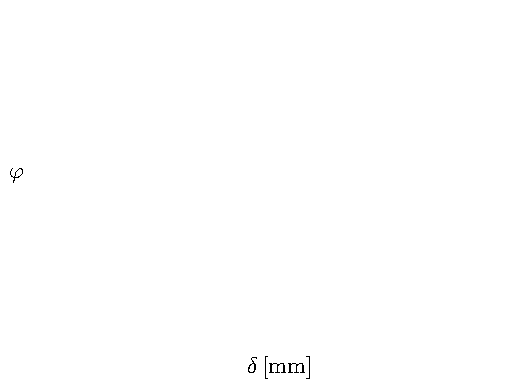
\includegraphics{P1/CeramBobineFat}
\CaptionFigs{Mesures représentant le rapport $\rapflux\equiv\ttfrac{\flux(\Devi)}{\flux(0)}$ des flux traversant la pièce en céramique avec et sans déviation, en fonction de l'amplitude $\Devi$ de la déviation hors de l'axe $z$ (selon l'axe $x$). Les valeurs négatives de $\Devi$ se rapportent à une déviation dans l'autre sens (vers les $x$ décroissants) et sont obtenues en changeant le sens du courant parcourant les bobines. On constate que si le jet est dévié de $\Devi\approx\CeramRay=\mm{1,5}$, tous les atomes sont éliminés.}
\label{fig:CeramBobineFat}
\efigh



\casse


\noindent Il est intéressant de discuter un point mis en évidence par la figure~\nref{fig:CeramBobineFat} : il apparait que la totalité des atomes sont éliminés sur la céramique si la trajectoire moyenne du jet est déviée de $\Devi\approx\CeramRay=\mm{1,5}$, \cad si celle-ci devient tangente à la surface. 
%
%\vspace{-0.6cm}


\subsubsection{Pouvions-nous prévoir ce résultat ?}
\inlinefig{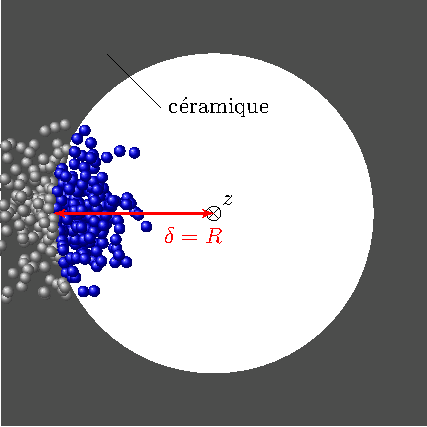
\includegraphics{P1/CeramAtomesDansCeram}} 
Dans le cas d'un nuage piégé, il semble évident que si le fond du piège est positionné au niveau de la surface ($\CeramDist~=~0$), tous les atomes vont y être éliminés après, au maximum, une demi-période d'oscillation. \label{Rq:PrevoirResultatDevi}

 Dans notre cas en revanche, le jet se propage suivant l'axe $z$ à une vitesse de \mps{1}. Ainsi, \emph{si la céramique était extrêmement fine} suivant l'axe $z$, seuls seraient éliminés les atomes qui se trouvent, au moment précis du passage dans la céramique, dans le demi-espace couvert par celle-ci. 
\noindent Sur le schéma ci-contre, qui représente une vue selon l'axe $z$, les atomes éliminés sont grisés. On s'attendrait donc à conserver environ la moitié des atomes (voir la figure \vref{fig:CeramBobineFatSimu}).
\picskip{0}
%\vspace{0.4cm}

\ApplicationNumerique
{
\noindent En réalité, la céramique possède une épaisseur $\CeramLong=\mm{5}$ suivant l'axe $z$. La vitesse moyenne du jet étant de $\vjet=\mps{1}$, chaque atome a besoin en moyenne d'un temps $\ttfrac{\CeramLong}{\vjet}=\ms{5}$ pour traverser la pièce de céramique. Ce temps est long devant la demi-période d'oscillation typiquement inférieure à \ms{0,5} (voir le chapitre~\nref{chap:JetAtomique}). C'est la raison pour laquelle tous les atomes sont éliminés pour une déviation d'amplitude $\Devi=\CeramRay=\mm{1,5}$.
}

\subsection{Gain en \ddedpup}\label{sec:ResultatVariationDDEDPUP}

Lorsqu'une partie des atomes les plus énergétiques du jet a été éliminée sur la \pdec, il s'en suit un retour vers un nouvel état d'\eqthdy%
\footnote{Nous avons en effet montré dans le chapitre~\nref{chap:JetAtomique} que le \jat que nous produisons possède un \tcolel suffisant pour autoriser la \reth.}%
.
Dans cette sous-section nous nous intéressons à la variation de température et de \ddedpup induite par le \fisp. 

\noindent Afin de mettre en évidence le refroidissement du jet, nous comparons toujours les résultats de deux mesures de température $T$, effectuées \m{3} en aval de la \pdec :
\begin{itemizel}
	\item une mesure $T(\Devi)$ correspondant au jet dévié d'une distance $\Devi$,
	\item et une mesure $T(\Devi=0)$ correspondant à la propagation habituelle du jet, \cad en l'absence de déviation. Dans notre cas, cette température est typiquement $T(0)=\microK{650}$.
\end{itemizel}



\Cahier{7,151}
\noindent Le tableau \vpageref[ci-dessous]{tab:CeramDDEDPUP} présente, pour différentes amplitudes $\Devi$ de déviation, quelques mesures expérimentales de rapports de températures 
$
\ttfrac{T(\Devi)}{T(0)}
%\virguleformule
$,
ainsi que les rapports de \fats
$
\rapflux=\ttfrac{\flux(\Devi)}{\flux(0)}
%\virguleformule
$
qui y sont associés. 

\noindent Ces deux données nous permettent de calculer%
\footnote{voir l'équation \vref{eq:rhojetaxe}.}
les gains correspondants pour la \ddedpup :
\[
%\GainDevi \equiv 
\frac{\rhojetaxe(\Devi)}{\rhojetaxe(0)}
\virguleformule
\]
où $\rhojetaxe$ désigne la \ddedpup sur l'axe du \jat:
\[
\setlength{\extrarowheight}{9 pt}\label{tab:CeramDDEDPUP}
\begin{array}{|c|c|c|c|c|}
\hline
   \Devi & 
   \mm{0,68} & \mm{0,79} & \mm{0,90} & \mm{1,0} \\
\hline
   \rapflux\equiv\frac{\flux(\Devi)}{\flux(0)} & 
   \val{0,88} & \val{0,82} & \val{0,71} & \val{0,60} \\
\hline
   \,\,\, \frac{T(\Devi)}{T(0)} \mbox{ avec } T(0)\approx\microK{650} \,\,\, & 
   \val{0,94}\pm\val{0,03} & \val{0,92}\pm\val{0,03} & \val{0,83}\pm\val{0,03} & \val{0,77}\pm\val{0,03} \\
\hline
   \frac{\rhojetaxe(\Devi)}{\rhojetaxe(0)} & 
   \val{1,08}\pm\val{0,09} & \val{1,09}\pm\val{0,09} & \val{1,34}\pm\val{0,11} & \val{1,50}\pm\val{0,12} \\
\hline
\end{array}
\]
\Resultat
{
%En utilisant une déviation de $\Devi=\mm{1,0}$ la température du jet obtenue après \reth est $T'=\microKpm{500}{10}$. La variation de \fat correspondant étant de $\rapflux=0,6$, nous
Nous pouvons donc obtenir un gain d'un facteur \val{1,5} en \ddedpup. Ceci s'accompagne d'une perte d'environ $10\%$ sur le \tcolel (voir la \autoref{sec:CeramSimuGainTcol}). Cette technique d'évaporation présente donc des performances comparables à l'évaporation par \firf décrite dans la \autoref{sec:EvapRf}.
}



\section{Dimensionnalité de l'évaporation}\label{sec:CeramBiDimensionnalité}
Comme nous l'avons mentionné dans la \autoref{sec:EvapCeramMiseEnOeuvre}, le processus d'évaporation par élimination sur une surface matérielle possède un caractère \emph{unidimensionnel}~\cite{HMO03} puisqu'il n'élimine les atomes qu'en fonction de l'un de leurs degrés de liberté en position%
\footnote{En toute rigueur, sur notre \setup, la surface interne de la céramique n'agit pas que sur un seul degré de liberté (suivant l'axe $x$). En effet, celle-ci n'est pas une surface plane~\cite{HMO03}, mais cylindrique. Elle agit donc aussi sur l'autre degré de liberté transverse (suivant l'axe $y$ dans notre cas).}
(suivant l'axe $x$ dans notre cas). 
On peut donc s'interroger sur son efficacité en terme de gain en \ddedpup. Nous pouvons en effet montrer que si l'évaporation concernait les deux degrés de liberté transverses, nous pourrions espérer un gain d'un facteur \val{3.4}~\cite{LaG05}.
%
Cette section a pour but de montrer pourquoi cette technique d'évaporation peu en fait aisément être rendue \emph{bidimensionnelle}.

\subsubsection{Redistribution de l'énergie mécanique transverse dans le \ppthyp}
Rappelons que le \ppt dans le \gm \emph{n'est pas de forme harmonique}, mais hyperbolique (voir la \autoref{sec:ConfigMagnetiqueGuide}). Le couplage entre les degrés de liberté transverses qui en résulte implique que les trajectoires atomiques projetées sur le plan transverse $(x,y)$ ne sont a priori pas des trajectoires fermées. La figure~\nref{fig:CeramTrajGuide_a} montre un exemple typique de trajectoire. On y voit bien la redistribution de l'énergie mécanique transverse suivant différentes directions du plan $(x,y)$ du fait que la trajectoire \sotosay{pivote}.

La figure~\nref{fig:CeramTrajGuide_b} montre d'ailleurs qu'une trajectoire atomique, qui n'atteindrait a priori pas la surface au moment où l'atome arrive au niveau de la céramique, peut en fait après un certain temps pivoter suffisamment pour l'atteindre.
%
\bfighss
\subfloat[]
{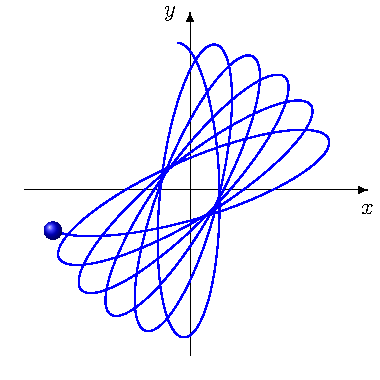
\includegraphics{P1/CeramTrajGuide_a}\label{fig:CeramTrajGuide_a}} \;
\subfloat[]
{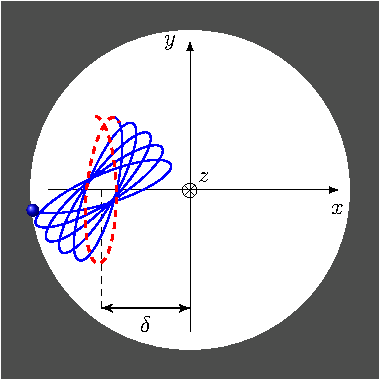
\includegraphics{P1/CeramTrajGuide_b}\label{fig:CeramTrajGuide_b}}
\CaptionFigs{Représentation d'une trajectoire atomique typique projetée dans le plan $(x,y)$. \\
(a) : Le \ppt non-harmonique fourni par le guide implique un couplage des degrés de liberté transverses. Ainsi, la direction pour laquelle l'atome est à l'apogée de sa trajectoire pivote au fil du temps. \\
(b) : Lorsqu'un atome pénètre dans le trou de la \pdec, sa trajectoire peut initialement ne pas atteindre la surface (partie rouge tiretée de la trajectoire). En effet, son énergie mécanique est essentiellement répartie selon la direction $y$. Cependant, au fil des oscillations, la trajectoire pivote et peut finir par atteindre la surface.% L'énergie mécanique est re-distribuée sur différente direction du plan ($x,y$).
}
\label{fig:CeramTrajGuide}
\efigh

\ifthenelse{\FormatEUE > 0}{}
{\AjouteLigne}
%
C'est cette redistribution au fil du temps de l'énergie mécanique sur différentes directions du plan $(x,y)$ qui peut rendre le processus d'évaporation presque aussi efficace que s'il était bidimensionnel. Il faut pour cela que les atomes restent suffisamment longtemps au niveau de la \pdec.
\Resultat
{
La \emph{dimensionnalité effective} de l'évaporation dépend de la longueur $\CeramLong$ de la \pdec suivant l'axe $z$ et de la vitesse moyenne $\vjet$ du \jat.
Pour nos paramètres expérimentaux typiques, une simulation numérique montre que l'évaporation serait considérée comme étant bidimensionnelle si la pièce de céramique avait une longueur d'au moins $\CeramLong=\cm{5}$ (voir la \autoref{sec:CeramSimuGain}).
}

\Remarque{Il convient de garder à l'esprit que la redistribution de l'énergie mécanique sur les degrés de liberté transverses est directement liée à l'anharmonicité du \ppt. Dans le cas d'un piégeage harmonique, les trajectoires sont toujours fermées, de forme elliptique.
Nous avons montré dans la \autoref{sec:ConfigMagnetiqueGuide} que la forme du potentiel auquel sont soumis les atomes dépend du facteur $\alpha$ défini à la \vpageref{Rq:alpha}.
% :
%%$\alpha = \ttfrac{\mu\,\Bpara}{\kb\,T}$ 
%\[
%\alpha = \alphaexpr
%\pointformule
%\]
Ainsi dans la perspective d'abaisser de plus en plus la température ($\alpha \ll 1$), nous finirons toujours par atteindre la limite d'un potentiel harmonique, et donc par annuler l'effet de bidimensionnalité décrit dans cette section.
}


\casse


\section{Interprétation des résultats}

Afin d'interpréter les variations de \fat en terme de \fispse, il serait utile de disposer d'une modélisation du problème. Cependant, dans le cas de l'évaporation du jet sur nos \pdecs, la formalisation du problème ne permet pas d'obtenir des résultats analytiques simples, et ce pour plusieurs raisons:
\begin{itemizel}
	\item le problème ne possède pas de symétrie de révolution autour de l'axe $z$ (contrairement au cas dans la \autoref{sec:MesureTempTrans} pour le \firf).
	\item Le \ppt n'est pas harmonique (voir la \autoref{sec:ConfigMagnetiqueGuide}). Comme nous l'avons vu, il en résulte un couplage entre les degrés de liberté transverses qui fait intervenir le temps passé au voisinage de la \pdec.
	\item la surface interne de la céramique n'est pas plane, mais cylindrique. Le critère de filtrage fait donc lui aussi intervenir les deux degrés de liberté transverses.
\end{itemizel}
Cette section a pour but de comparer nos résultats expérimentaux avec ceux obtenus grâce à des simulations numériques. Nous commençons, dans la sous-section suivante par décrire les \emph{ingrédients physiques} utilisés dans ces simulations.

\subsection{Simulations numériques}\label{sec:CeramSimu}
Les simulations numériques ont été effectuées par Antoine Couvert dans le cadre de son stage de DEA. La programmation en langage \termetech{Fortran 95}, met en \oe uvre une méthode de \termetech{Monte-Carlo} associée à un algorithme symplectique d'ordre~4~\cite{Yos93} pour calculer la trajectoire des atomes. 
Mentionnons que la simulation \emph{ne tient pas compte des \colels entre atomes}. Nous justifions cette simplification par le fait que les atomes restent au voisinage de la \pdec pendant typiquement \ms{5} (voir \vpageref{Rq:PrevoirResultatDevi}), alors que le \tcolel par atome est seulement de l'ordre de $\SI{10}{\reciprocal\second}$.
% \ll \ttfrac{1}{\val{0.005}}=\SI{200}{\reciprocal\second}$.

\noindent Les positions et vitesses initiales des atomes sont tirées aléatoirement par la méthode de réjection~\cite{PTV92} de manière à reproduire les grandeurs physiques qui caractérisent notre \jat, et que nous déterminons expérimentalement:
\begin{itemizel}
	\item la vitesse moyenne du jet $\vjet=\mps{1,0}$,
	\item sa température d'\eqthdy $T=\microK{650}$,
	\item le \gtchm imposé par le guide $\gradB=\gausspcm{800}$,
	\item le champ longitudinal $\Bpara=\gauss{1}$,
	\item la géométrie de la surface cylindrique de rayon $\CeramRay=\mm{1,5}$ et de longueur $\CeramLong=\mm{5}$.
\end{itemizel}
Pour reproduire le critère de \fispse, nous supposons que le jet se propage suivant une ligne droite (l'axe $z$), et qu'il passe au travers d'une \pdec qui, elle, est désaxée latéralement d'une distance $\Devi$. 
Nous supposons une \emph{efficacité d'évaporation de $100\%$}. Ainsi, toute trajectoire atteignant la surface du cylindre de rayon $\CeramRay=\mm{1,5}$, de longueur $\CeramLong=\mm{5}$ et dont l'axe est excentré d'une distance $\Devi$ par rapport à la trajectoire moyenne du jet, est considérée comme étant éliminée.


\casse


\subsection{Variation du \fat}

La figure~\nref{fig:CeramBobineFatSimu} représente les données expérimentales de la figure~\nref{fig:CeramBobineFat} (page \pageref{fig:CeramBobineFat}) ainsi que le calcul de $\rapflux$ obtenu par la simulation numérique. 
\bfighs
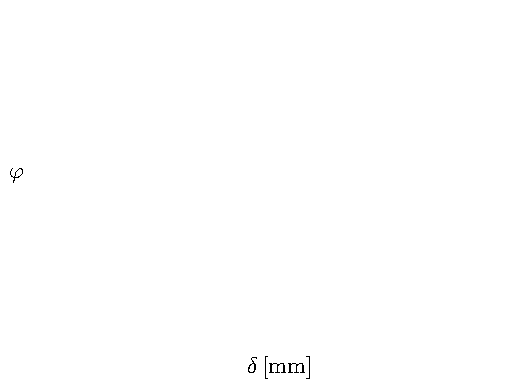
\includegraphics{P1/CeramBobineFatSimu}
\CaptionFigss{Représentation des variations du \fat en fonction de l'amplitude $\Devi$ de la déviation. Les données expérimentales de la figure~\nref{fig:CeramBobineFat} (page \pageref{fig:CeramBobineFat}) sont représentées par des carrés grisés. Les résultats de la simulation pour la fraction $\rapflux \equiv \ttfrac{\flux(\Devi)}{\flux(0)}$ sont représentés par une ligne continue. 
%Toutes les grandeurs physiques qui caractérisent le jet, le confinement et la géométrie de la pièce de céramique sont entrées dans la simulation telles qu'elles sont mesurées expérimentalement. Le seul ajustement effectuer sur le résultat de la simulation est un déplacement global de la courbe de \micron{-40} sur l'axe des abscisses. Ceci traduit simplement le fait que le trou central de la pièce de céramique utilisée est très légèrement désaxée par rapport à l'axe $z$.\\
La ligne pointillée représente le résultat de la simulation pour $\rapflux$ mais en considérant le cas d'une pièce de céramique de \emph{longueur extrêmement faible} ($\CeramLong=\micron{10}$). Dans ces conditions, comme nous l'avons mentionné dans la \autoref{sec:ResultatVariationFlux}, les atomes n'ont pas le temps d'effectuer une demi-période d'oscillation lors de la traversée de la céramique. On constate d'ailleurs, comme prévu dans ce cas, que pour une déviation d'amplitude $\Devi=\CeramRay=\mm{1,5}$, environ la moitié des atomes sont éliminés.
}
\label{fig:CeramBobineFatSimu}
\efigh


%\Remarque
{\label{Rq:DeviZero}
Rappelons que $\rapflux\equiv\ttfrac{\flux(\Devi)}{\flux(0)}$ est le rapport du flux traversant la céramique en présence d'une déviation $\Devi$ par le flux en l'absence de déviation ($\Devi=0$). 
Il est en effet important de ne pas confondre les deux grandeurs suivantes :
\begin{itemize}
	\item le flux \emph{traversant la céramique en l'absence de déviation} 
	\item et le flux \emph{en l'absence pur et simple de céramique}. 
\end{itemize}
%La deuxième de ces grandeurs n'est pas expérimentalement mesurable puisque les céramiques sont dans l'enceinte à vide. 
}
En outre, la simulation numérique montre que, \emph{même en l'absence de déviation}, le \fat est réduit d'environ $4\%$.
Ceci est dû au fait que, dans la gamme de température dans laquelle nous nous trouvons ($\approx\microK{650}$), la pièce de céramique élimine les atomes qui sont suffisamment énergétiques pour que leurs trajectoires s'éloignent de plus de $\CeramRay=\mm{1,5}$ de l'axe du guide. On s'attend à voir disparaître cet effet lorsque la température du jet est plus faible.
%\Resultat
%{}

Au vu de l'excellent accord avec les données expérimentales, il est important de rappeler que toutes les grandeurs physiques utilisées dans la simulation ont été mesurées expérimentalement. Il n'y a donc aucun paramètre ajustable, si ce n'est l'efficacité d'évaporation, que nous avons supposée de $\val{100}\%$.

\Remarque{
En fait, le seul ajustement effectué sur le résultat de la simulation correspond à déplacer globalement la courbe de la figure~\nref{fig:CeramBobineFatSimu} sur l'axe des abscisses. Ceci rend compte d'un léger parallaxe entre le trou central de la céramique et l'axe $z$.
Nous avons ainsi constaté que la pièce en céramique que nous utilisons pour nos expériences possède un trou désaxé de \micron{40} par rapport à l'axe du \gm.
}

\ifthenelse{\FormatEUE > 0}{}
{\AjouteLigne \AjouteLigne}

\subsection{Gain en \ddedpup}\label{sec:CeramSimuGain}
Intéressons nous maintenant à l'évolution des caractéristiques du jet après la traversée de la \pdec. La simulation ne tient pas compte des \colels entre atomes, qui sont indispensables pour accéder à la dynamique de la \reth. 
Nous pouvons néanmoins supposer qu'après le \fisp, le jet atteint un nouvel état d'\eqthdy, et effectuer un simple bilan d'énergie afin de déduire le gain $\GainCeram$ en \ddedpup:
%\RemonteUnPeuFig
\[
%\Delta\rhojetaxe \equiv 
\GainCeram \equiv \frac{\AvecTexte{\rhojetaxe}{après}}{\AvecTexte{\rhojetaxe}{avant}}
\virguleformule
\]
où $\AvecTexte{\rhojetaxe}{avant}$ et $\AvecTexte{\rhojetaxe}{après}$ sont les \ddedpup sur l'axe du jet, respectivement avant traversée de la céramique et après traversée de la céramique suivie d'une \reth.
% (voir la \autoref{sec:RethermJet}). 

La simulation permet de nous intéresser à des situations pour lesquelles la longueur $\CeramLong$ de la céramique serait différente de \mm{5}. 
La figure~\nref{fig:CeramBobineDDEDPUPSimu} représente les gains $\GainCeram$ en \ddedpup obtenus après \reth, et en considérant $\CeramLong=\micron{10}$, $\CeramLong=\mm{5}$, $\CeramLong=\mm{10}$ et $\CeramLong=\mm{100}$.
%
\bfighs
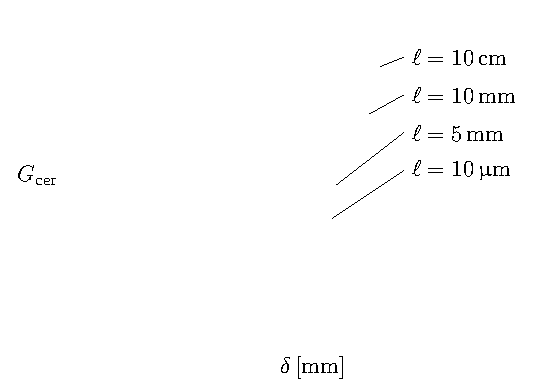
\includegraphics{P1/CeramBobineDDEDPUPSimu}
\RemonteUnPeuFig
\RemonteUnPeuFig
\CaptionTocCaptionFig{Représentation des résultats de la simulation numérique pour le gain en \ddedpup }{Représentation des résultats de la simulation numérique pour le gain en \ddedpup $\GainCeram%\equiv \ttfrac{\AvecTexte{\rhojetaxe}{après}}{\AvecTexte{\rhojetaxe}{avant}}
$ en fonction de la distance $\Devi$ de déviation. Les différentes courbes correspondent à différentes longueurs de la \pdec. On voit bien le caractère bidimensionnel de l'évaporation qui se manifeste avec l'augmentation de la longueur $\CeramLong$, comme mentionné en \autoref{sec:CeramBiDimensionnalité} (la ligne pointillée correspond précisément à une évaporation bidimensionnelle parfaite).
%Les symboles carrés correspondent à des données mesurées expérimentalement et sont donc à comparer à la courbe $\CeramLong=\mm{5}$.
}
\label{fig:CeramBobineDDEDPUPSimu}
\efigh

\casse

\subsubsection{Interprétation des résultats de la simulation numérique}\label{sec:CeramBobineDDEDPUPSimuInterpretation}
\noindent Proposons nous d'interpréter les résultats de la simulation présentés sur la figure~\nref{fig:CeramBobineDDEDPUPSimu}. On peut noter plusieurs points mis en évidence sur cette figure :
\begin{ditemize}
	\item comme prévu (voir la \autoref{sec:CeramBiDimensionnalité}), le caractère bidimensionnel de l'évaporation se manifeste lorsque nous prenons des longueurs $\CeramLong$ de plus en plus élevées. Pour $\CeramLong=\cm{10}$, on atteint quasiment les performances d'un processus d'évaporation à deux dimensions (ligne pointillée de la figure~\nref{fig:CeramBobineDDEDPUPSimu}).
	\item on constate que, \emph{même en l'absence de déviation} ($\Devi=0$), la \ddedpup du jet augmente sensiblement ($\approx+15\%$) du fait du passage dans la pièce de céramique. Ceci est la conséquence, comme nous l'avons noté dans la remarque \vpageref[ci-dessus]{Rq:DeviZero}, de l'élimination d'atomes suffisamment énergétiques pour qu'ils s'éloignent de plus de $\CeramRay=\mm{1,5}$ de l'axe $z$ du guide (le \fat est réduit d'environ $4\%$). 
	\item toutes les courbes (sauf pour $\CeramLong=\micron{10}$) convergent, quand $\Devi\rightarrow0$, vers la même valeur ($\approx\val{1.15}$) qui correspond aussi à celle obtenue pour une évaporation parfaitement bidimensionnelle. Ceci est prévisible dans la mesure où, si $\Devi=0$, la description du problème possède une symétrie de révolution. Le critère de \fisp et donc l'évaporation sont donc nécessairement bidimensionnels.
	\item la courbe correspondant à $\CeramLong=\micron{10}$ ne converge pas vers la même valeur que les autre quand $\Devi\rightarrow0$. En effet, comme nous l'avons vu dans la \autoref{sec:ResultatVariationFlux}, \emph{si la céramique est extrêmement fine}, les atomes n'ont pas le temps d'effectuer une demi-période d'oscillation au moment du passage dans celle-ci. N'est alors éliminé qu'une partie des atomes énergétiques qui devraient l'être.
	\item ce dernier point est d'ailleurs souligné par le fait qu'en $\Devi=\CeramRay=\mm{1,5}$, la totalité des atomes semblent être éliminés pour $\CeramLong \geqslant \mm{5}$, mais pas pour $\CeramLong=\micron{10}$ (voir \vpageref{Rq:PrevoirResultatDevi}).
\end{ditemize}



\subsubsection{Comparaison aux résultats expérimentaux}

Nous allons comparer les données de la simulation numérique aux résultats expérimentaux de la \autoref{sec:ResultatVariationDDEDPUP}. Il faut pour cela tenir compte d'un des points mentionnés ci-dessus : 
\emph{même en l'absence de déviation} ($\Devi=0$), la \ddedpup du jet augmente sensiblement.
Sur notre expérience, il est impossible de mesurer l'influence réelle d'une des \pdecs sur le jet puisque celles-ci sont placées dans l'enceinte à vide et ne peuvent donc pas être retirées du \setup. 
\inlinefig{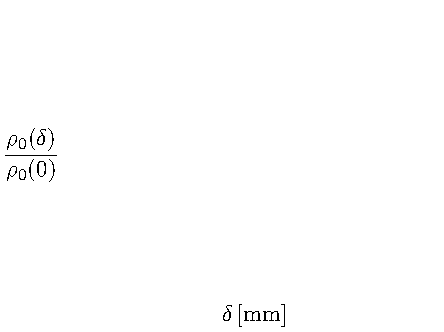
\includegraphics{P1/CeramBobineDDEDPUPSimuExp}} 
\noindent Dans la pratique, nous mesurons en fait le gain en \ddedpup en comparant l'effet d'une céramique avec une déviation d'amplitude $\Devi$ à l'effet de la même céramique sans déviation ($\Devi=0$). En d'autres termes, nous ne mesurons pas :
\[
\GainCeram 
\equiv \frac{\rhojetaxe(\Devi)}{\AvecTexte{\rhojetaxe}{sans céramique}}
\virguleformule
\mbox{ mais }\frac{\rhojetaxe(\Devi)}{\rhojetaxe(0)}
\pointformule
\]
\noindent La figure ci-contre représente les résultats de la simulation numérique pour  $\tfrac{\rhojetaxe(\Devi)}{\rhojetaxe(0)}$ (ligne continue), ainsi que les points mesurés expérimentalement.


\casse


\subsubsection{Influence des autres pièces de céramiques}
Il convient de mentionner que la grandeur physique à laquelle nous avons accès sur notre \setup n'est en fait pas exactement $\ttfrac{\rhojetaxe(\Devi)}{\rhojetaxe(0)}$. En effet, notre guide ne comporte pas qu'une seule pièce de céramique, mais une dizaine, réparties tous les \cm{40} environ. 
Pour notre étude nous utilisons \emph{l'une de ces céramiques}, placée environ \m{1} après l'entrée du guide. Ceci implique en outre que le \jat, au moment où il passe à travers \emph{cette} céramique, est déjà passé à travers d'autres pièces avant et en traversera d'autres après. 

\Resultat
{
Nous avons vu que, dans cette gamme de température ($\approx\microK{600}$), chaque céramique a un effet sur le jet, même si celui-ci n'est pas dévié. 
Nous mesurons donc toujours l'influence de toutes les céramiques, \emph{dont l'une seulement} est en présence d'une déviation d'amplitude $\Devi$ du \jat. 
}

De plus, cela veut dire que le jet est en permanence maintenu légèrement hors d'\eqthdy, puisque chaque céramique tronque partiellement la distribution atomique. Le jet n'a en effet pas le temps de \rether entre deux céramiques successives. La simulation numérique décrite dans la \autoref{sec:CeramSimu}, elle, ne rend pas compte de l'influence de toutes les céramiques puisqu'elle ne fait pas intervenir les processus collisionnels.


\subsection{Gain en \tcolel}\label{sec:CeramSimuGainTcol}
Dans le chapitre~\nref{chap:JetAtomique} nous avons souligné l'importance de maintenir un \tcolel soutenu au sein du jet. La figure~\nref{fig:CeramBobineGammaSimu} représente les résultats de la simulation numérique pour le gain en \tcolel 
$
\ttfrac{\gammacolapres}{\gammacol}
%\virguleformule
$
obtenu après \reth, en considérant comme précédemment $\CeramLong=\micron{10}$, $\CeramLong=\mm{5}$, $\CeramLong=\mm{10}$ et $\CeramLong=\mm{100}$.
%
\bfighs
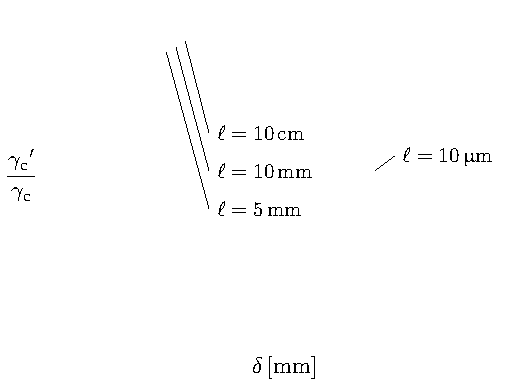
\includegraphics{P1/CeramBobineGammaSimu}
\CaptionFigss{Représentation des résultats de la simulation numérique pour le gain en \tcolel $\ttfrac{\gammacolapres}{\gammacol}$ en fonction de la distance $\Devi$ de déviation. Les différentes courbes correspondent à différentes longueurs de céramique. Le caractère \bd de l'évaporation mentionné en \autoref{sec:CeramBiDimensionnalité} permet d'augmenter substantiellement le \tcolel.
}
\label{fig:CeramBobineGammaSimu}
\efigh

\casse

Nous constatons sur la figure~\nref{fig:CeramBobineGammaSimu} qu'il est possible d'augmenter sensiblement le \tcolel : $6\%$ dans nos conditions expérimentales et jusqu'à $10\%$ pour une évaporation quasi-\bde%
%\footnote
{% 
. Cependant, pour obtenir les gains maximaux mentionnés ci-dessus (respectivement $6\%$ et $10\%$), il faut se contenter alors de gains plus modestes pour la \ddedpup (respectivement $1,3$ et $1,7$ environ)~\cite{LaG06}.
}%
\noindent Notons que les remarques faites sur la figure~\nref{fig:CeramBobineDDEDPUPSimu} (page \pageref{sec:CeramBobineDDEDPUPSimuInterpretation}) sont aussi valables pour la figure~\nref{fig:CeramBobineGammaSimu}.

\Resultat{La déviation du jet au niveau d'une \pdec permet en principe d'augmenter significativement le \tcolel, tout particulièrement si l'élimination est rendu \bde. Rappelons toutefois (voir la \autoref{sec:RethermJet}) que ce point est directement lié au fait que le \ppt n'est pas harmonique.}




\section{Déviation du jet à l'aide d'aimants permanents}\label{sec:EvapCeramAimants}
Nous avons décrit dans la \autoref{sec:EvapCeramMiseEnOeuvre} comment dévier la trajectoire moyenne du \jat à l'aide d'une paire de bobines positionnée symétriquement de part et d'autre du guide. Nous pouvons ainsi contrôler l'amplitude $\Devi$ de la déviation avec une grande précision.
Dans la perspective d'utiliser un grand nombre de zones d'évaporation, ce dispositif souffre cependant de quelques défauts :
\begin{itemize}
	\item l'encombrement spatial des bobines (d'environ \cm{10} suivant l'axe du guide) rend difficile l'enchainement de zones d'évaporation,
	\item la fabrication d'un grand nombre de bobines peut rendre la mise en pratique fastidieuse,
	\item il est nécessaire de disposer d'autant de sources de courant stabilisées que de paires de bobines.
\end{itemize}

Cette section a pour but de présenter brièvement une mise en \oe uvre beaucoup plus compacte de la méthode d'évaporation du jet sur une surface. Celle-ci, se basant sur l'utilisation d'aimants permanents, est bien moins onéreuse et sa mise en \oe uvre est rapide (pas de bobines à fabriquer, pas besoin d'alimentations stabilisées).

\subsection{Mise en \oe uvre}
\Cahier{8,62-65}
Dans cette sous-section nous décrivons brièvement le \setup qui nous permet d'évaporer le \jat sur une céramique à l'aide d'aimants permanents.
Tout comme nous l'avons vu dans la \autoref{sec:EvapCeramBobines}, il est important de produire une configuration antisymétrique de \chm par rapport à l'axe $z$ afin de ne pas produire de colline de potentiel le long du trajet du jet. 

\inlinefig{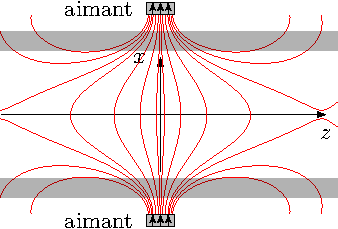
\includegraphics{P1/GuideChampTransMagnets}} 
Les aimants que nous utilisons sont composés d'un alliage de Niobium (Nb-Fe-B). L'annexe~\nref{annexe:ModelisationAimants} précise leurs caractéristiques. Deux aimants sont montés de manière symétrique, de part et d'autre du guide, au niveau de l'une des céramique. Les aimantations sont dirigées dans le même sens, suivant les $x$ croissants dans notre cas. La figure ci-contre représente quelques lignes du \chm ainsi produit dans le plan ($x,z$).
\noindent Afin de contrôler précisément l'écart $\Daimants$ entre les deux aimants, ceux-ci sont fixés sur des platines de micro-positionnement (voir la figure~\nref{fig:EvapMagnet}). 
Nous pouvons ainsi faire varier $\Daimants$ sur une plage de $58$ à $\mm{90}$. 
%La  représente une photographie du montage.
\picskip{0}
%
\bfigh
\RemonteUnPeuFig
{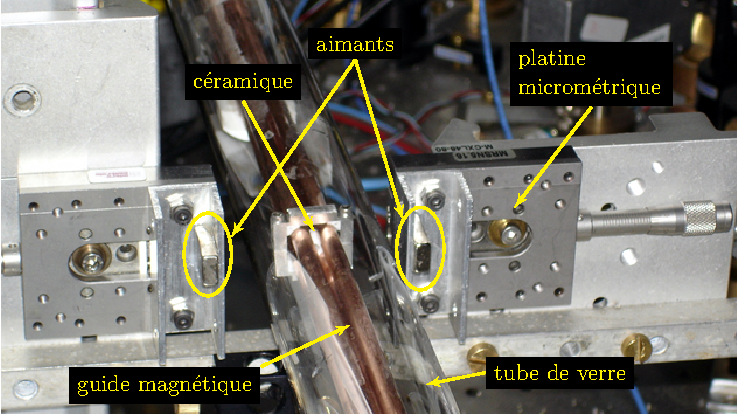
\includegraphics[scale=1]{P1/CeramEvapMagnets}}
\RemonteUnPeuFig
\CaptionFig{
(b) : photographie du \setup permettant d'évaporer le \jat sur une pièce de céramique. On y voit une portion du \gm sur laquelle se trouve l'une des pièces de céramique. De part et d'autre du guide, les deux platines de micro positionnement permettent d'ajuster la distance séparant les aimants de \mm{58} à \mm{90}.
}
\label{fig:EvapMagnet}
\efigh

\ifthenelse{\FormatEUE > 0}{}
{\AjouteLigne}

\subsection{Calibration du \chm produit par les aimants}
Afin de connaître précisément l'amplitude $\Devi$ de la déviation du jet il est impératif de calibrer la valeur du \chm transverse $\CeramBtrans$ imposé par les aimants au voisinage de l'axe $z$ du guide.
Celle-ci dépend naturellement de l'écart $\Daimants$ entre les deux aimants. La figure~\nref{fig:CeramAimantChamp} représente les mesures du \chm transverse 
%prises au long de l'axe $z$ pour différents écart $\Daimants$, ainsi que la valeur maximale $\Btransmax$, au niveau de la pièce de céramique, 
en fonction de $\Daimants$. 
\bfighsss
\subfloat[]{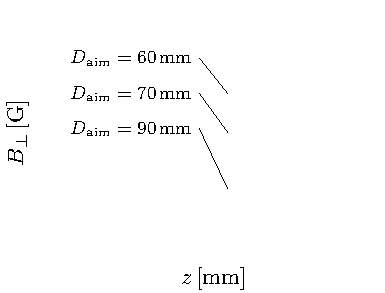
\includegraphics{P1/CeramAimantChampZ}}\,\,\,\,\,\,
\subfloat[]{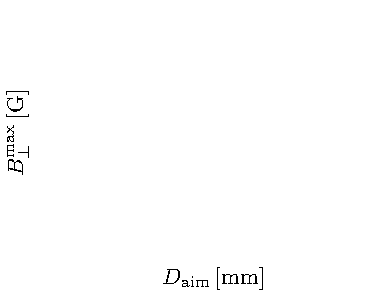
\includegraphics{P1/CeramAimantChampMax}}
\CaptionFigss{
(a) : mesure du \chm transverse $\CeramBtrans$ produit par les aimants en fonction de la position sur l'axe $z$. L'abscisse $z=0$ correspond à la position de la \pdec. Chaque courbe correspond à un écartement $\Daimants$ différent.\\
(b) : mesure du \chm transverse $\Btransmax$ produit au niveau de la \pdec en fonction de l'écart entre les aimants. La valeur $\Btransmax$ donne l'amplitude de la déviation $\Devi$ au niveau de la céramique grâce à la relation \vref{eq:Devi}.}
\label{fig:CeramAimantChamp}
\efigh

%Rappelons que c'est $\Btransmax$ qui donne l'amplitude de la déviation $\Devi$ grâce à la relation \vref{eq:Devi}.

\casse

\subsection{Variation du \fat}\label{sec:ResultatVariationFluxAimants}
Afin de valider cette technique se basant sur l'utilisation d'aimants permanents, nous la comparons brièvement à celle basée sur l'utilisation de bobines. 
Dans cette sous-section, nous présentons donc l'effet de ce dispositif sur le jet en terme de réduction du \fat, comme dans la \autoref{sec:ResultatVariationFlux}. 
La figure \vref{fig:CeramAimantFat} témoigne de l'équivalence de ces deux méthodes.
\bfighs
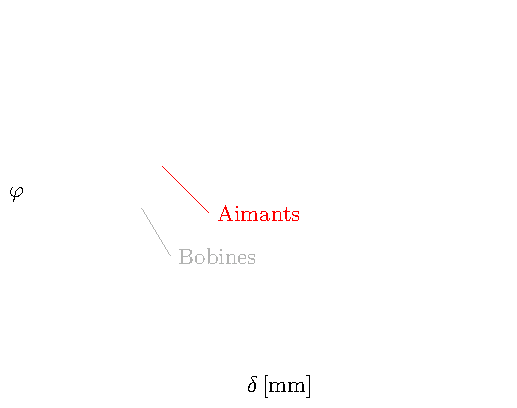
\includegraphics{P1/CeramAimantFat}
\CaptionFigss{Comparaison entre l'utilisation de bobines et l'utilisation d'aimants permanents. Nous représentons la réduction relative de \fat $\rapflux\equiv\ttfrac{\flux(\Devi)}{\flux(0)}$ des flux traversant la pièce en céramique avec, et sans déviation, en fonction de l'amplitude $\Devi$ de la déviation. \\
Les carrés grisés représentent les données de la figure \vref{fig:CeramBobineFat} (utilisation de bobines). \\
Les ronds rouges correspondent aux mesures effectuées en déviant la trajectoire à l'aide d'aimants permanents. Le \fat sans déviation est mesuré en retirant le dispositif représenté sur la figure~\nref{fig:EvapMagnet}.
Les valeurs négatives de $\Devi$ se rapportent à une déviation dans l'autre sens et sont obtenues en inversant l'orientation du dispositif.}
\label{fig:CeramAimantFat}
\efigh

\RemonteUnPeuFig
\RemonteUnPeuFig

\section{Conclusion}
Dans ce chapitre, nous avons présenté une technique permettant de mener à bien l'\evap d'un \jatmg. Nous avons adapté le principe d'élimination d'atomes énergétiques au contact d'une surface matérielle~\cite{HMO03} à notre \setup. Pour cela nous dévions localement la trajectoire du jet vers l'une des \pdecs présente dans notre \gm. 

\noindent Le contrôle de la déviation est assuré par la superposition local d'un \chm $\CeramBtrans$ transverse à l'axe du guide. 
Deux techniques sont présentées afin de produire ce champ:
\begin{itemizel}
	\item l'une se basant sur l'utilisation de bobines, 
	\item l'autre à base d'aimants permanents.
\end{itemizel}


%\casse

Ce processus d'évaporation peut, dans certaines conditions, être aisément rendu bidimensionnel et présente plusieurs avantages majeurs en comparaison de l'évaporation par \firf décrit dans le chapitre~\nref{chap:JetAtomique}:
\begin{itemizel}
	\item l'efficacité de l'élimination des atomes répondant au critère de filtrage est de $100\%$,
	\item l'action de \fisp est beaucoup plus locale puisqu'elle se produit au contact de la surface, soit quelques millimètres de long dans notre cas.
\end{itemizel}



%\subsubsection{Ouverture, possibilité de miniaturisation}
Concluons ce chapitre en soulignant un dernier point relatif à cette technique. Jusqu'ici nous avons décrit le cas d'un jet dévié de l'axe $z$ du \gm afin de lui faire approcher la surface d'une \pdec. 
\inlinefig{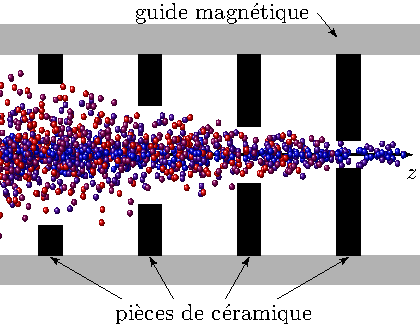
\includegraphics{P1/CeramPetitPetit}} 
Essayons d'imaginer un \setup qui serait optimisé pour pouvoir utiliser au mieux cette technique d'évaporation. Nous pourrions par exemple envisager de ne plus dévier le jet de son axe, mais plutôt d'utiliser tout au long du guide des céramiques dont le trou central serait de plus en plus étroits au fur et à mesure de la propagation. L'illustration ci-contre schématise cette idée en représentant un \jat se propageant suivant l'axe $z$ et passant à travers quatre \pdecs. Chacune d'elles élimine des atomes dont l'énergie est de plus en plus faible. 
\picskip{0}
Cet agencement, qui possède une symétrie de révolution, présente l'énorme avantage de produire une \emph{évaporation strictement \bde}, quelles que soient les conditions de piégeage et de température du jet. 
Sur un plan purement technique en revanche, ce type de dispositif est \emph{très peu flexible} puisqu'une fois placé dans un environnement \uv, il serait difficile d'ajuster la géométrie du système. L'espacement et les diamètres des céramiques devraient alors être calculés à l'avance, pour des caractéristiques initiales du jet très précises (en termes de flux, température, vitesse moyenne, confinement). 

\ifthenelse{\FormatEUE > 0}{}
{\AjouteLigne}

Pour prolonger cette idée, pourquoi ne pas envisager l'optimisation et la miniaturisation de ce type de structure? 
La figure~\nref{fig:CeramContinue} illustre l'utilisation d'une unique surface à symétrie de révolution dont la forme serait optimisée pour mener à bien le \rpef d'un \jatmg. L'encombrement total du système serait fonction uniquement des caractéristiques du jet incident, et non plus des contraintes liées à la portée d'une antenne \rf ou encore à l'encombrement de bobines. 
%Cette idée est à mettre en regard d'expériences effectuées dans le groupe d'Eric Cornell (\nomofficiel{University of Colorado}), et qui consistent à guider des atomes à l'intérieur de fibres optiques creuses~\cite{RMV95,MCA00}.
\bfighs
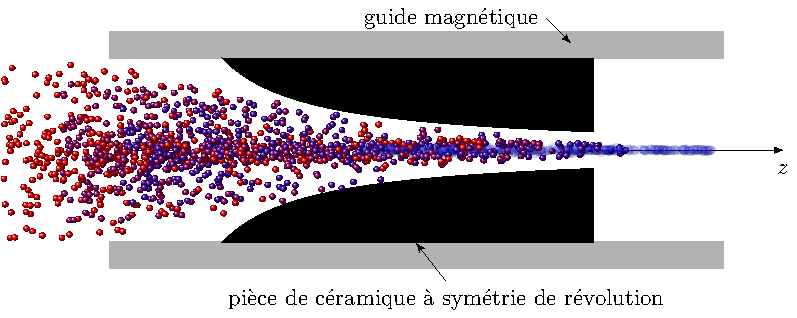
\includegraphics{P1/CeramContinue}
\CaptionFigss{Illustration d'une idée de principe. Une unique surface à symétrie de révolution à l'intérieur de laquelle peut se propager un \jatmg. La forme de cette surface serait optimisée afin de refroidir un jet ayant des caractéristiques données. Si ces dernières le permettent, la surface pourrait même être vue comme un système \sotosay{compact} acceptant un jet thermique \sotosay{en entrée} et fournissant \sotosay{en sortie} un faisceau de matière dans le \rdq.}
\label{fig:CeramContinue}
\efigh




}{}
%%%%%%%%%%%%%%%%%%%%%%%%%%%%%%%%%%%%%%%%%%%%%%%%%%%%%%%%%%%%%%%%%%%%%%%%%%%%%%%%%%%%%%%%%%
%%%%%%%%%%%%%%%%%%%%%%%%%%%%%%%%%%%%%%%%%%%%%%%%%%%%%%%%%%%%%%%%%%%%%%%%%%%%%%%%%%%%%%%%%%
%%%%%%%%%%%%%%%%%%%%%%%%%%%%%%%%%%%%%%%%%%%%%%%%%%%%%%%%%%%%%%%%%%%%%%%%%%%%%%%%%%%%%%%%%%
%
%\PutNewPageInToc
%
\ifthenelse{\IncludePartTwo > 0}{
\DontNumberThisInToc
\part{\TitrePartieDeux}
\chapter{\TitreChapitreTrois}\label{chap:MiroirMobile}

\bfigh
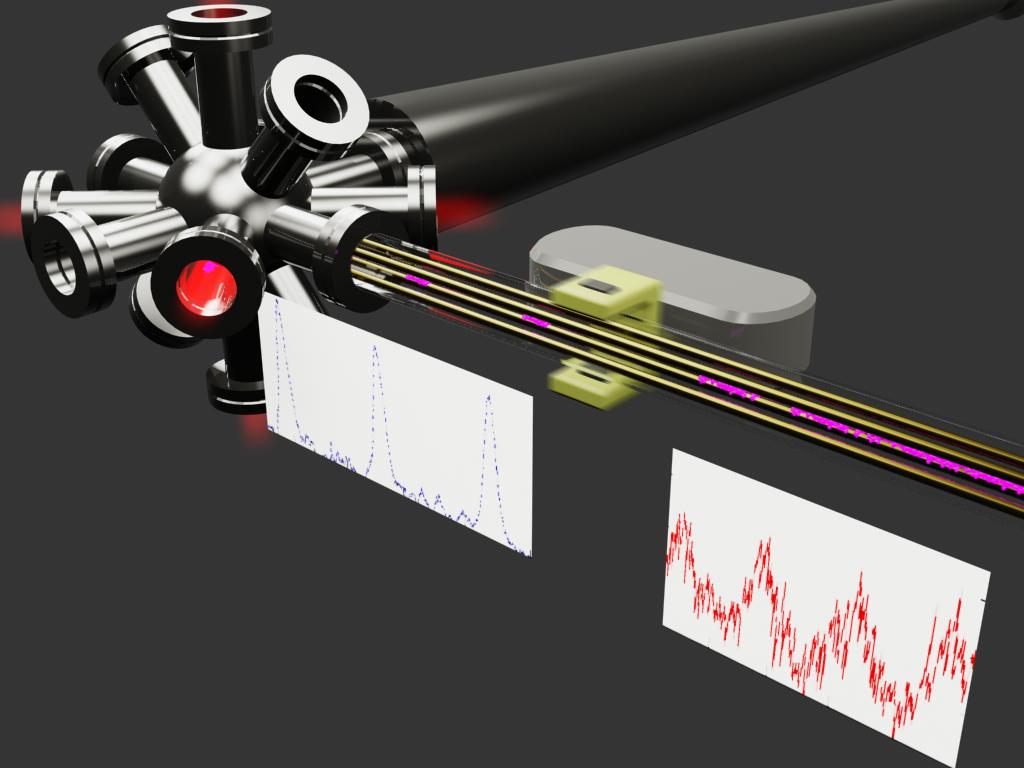
\includegraphics[width=\FigWidth]{P2/ChapitreMiroir}
{Représentation du \mimo utilisé sur notre \gm. Cette image a été publiée dans la section \nomofficiel{Highlight} de la revue EuroPhysics News afin d'illustrer les résultats de notre article~\cite{RWC06}.}%
% dont le résumé est fourni en annexe~\nref{annexe:Articles}.}%, \emph{A moving magnetic mirror to slow down a bunch of atoms}, joint en annexe.}
%\label{fig:MiroirEPN}
\efigh

\pagebreak

\minitoc

\section{Introduction}
Dans la première partie de ce manuscrit nous avons abordé le problème de la formation d'un \jatg, intense et lent. Rappelons-en ici les points importants qui nous seront utiles dans ce chapitre:
\begin{itemizel}
	\item l'injection pulsée de \pats dans le \gm permet d'obtenir des flux atomiques importants. L'optimisation de ce flux nous mène à l'utilisation de \emph{vitesses d'injection assez élevées} (typiquement \mps{1}).
	\item à l'inverse, nous avons tout intérêt à disposer d'un \jat (qui résulte du recouvrement des \pats) dont la \emph{vitesse moyenne est faible}, de manière à disposer d'un temps suffisant pour mener à bien le processus d'évaporation forcée. Corrélativement, pour un flux donné, un jet lent est linéiquement plus dense et chaque atome subit ainsi un nombre accru de collisions lors de sa propagation.
\end{itemizel}
Nous avons décrit une manière de concilier ces points, en ralentissant les atomes grâce à la mise en place d'une \secpent du \gm. Cette technique souffre cependant d'un défaut majeur : le ralentissement et la compression linéique du \jat s'accompagnent d'un échauffement et d'une mise hors d'\eqthdy de celui-ci.

\casse

Ce chapitre présente le ralentissement de \pats injectés dans le \gm par réflexion spéculaire sur un \mimamo. %Il est organisé de la manière suivante: 
Nous commencerons par souligne les limites liées à l'utilisation d'une \secpent comme moyen de ralentissement d'un \jat (voir l'annexe~\nref{annexe:SectionPentue}).
Après avoir introduit le principe de notre technique, et décrit la mise en \oe uvre expérimentale du \mima, nous présentons les résultats expérimentaux relatifs au ralentissement d'un \pat.
Finalement, nous discuterons nos résultats dans le contexte plus spécifique de l'utilisation de cette technique pour la formation d'un \jatuf et lent. 

La fin de ce chapitre sera consacrée à l'étude d'un point particulier de ce procédé de ralentissement. Celui-ci rend en effet possible l'obtention d'un jet ayant une \ddedp plus élevée que ce que nous obtiendrions grâce à l'utilisation d'une \secpent.
Ce point sera mis en regard du \thLi et nous amènera à considérer l'action du \mimo sur les \ps comme celle d'un \termetech{démon de Maxwell} (voir l'annexe~\nref{annexe:ThLi}).


\section{Limites du ralentissement par une \secpent}\label{sec:LimitePente}


Le fait de faire gravir une pente au \jat a bien pour effet de le ralentir, mais ceci se fait au prix d'un échauffement du jet, ou plus précisément, au prix d'une augmentation de la \dispvitlong. 

Le \thLi qui s'applique à tout système mécanique subissant une évolution hamiltonienne implique que, dans le cas d'un potentiel indépendant du temps, la \ddedp
reste constante le long de toute trajectoire. 
En d'autres termes, en suivant une particule dans son mouvement, la \fdd dans l'\edp qui l'environne reste constante. 
Rappelons que (d'après l'expression~\nref{eq:rhojetaxe} définie page \pageref{eq:rhojetaxe}) la \ddedp $\rhojetaxe$ suivant l'axe du \j suit la relation de proportionnalité%
\footnote{Toutes autres choses étant égales par ailleurs et en considérant le \pptlin, \cad avec le paramètre $\alpha = 0$.} :
\[
	\rhojetaxe \equiv \njetaxe \, \lambdaDB^3 
	\propto \frac{\flux}{\vjet\,T^\ttfrac{7}{2}} 
	\pointformule
\]
Or, pour un \j en régime stationnaire, le flux $\flux$ est constant lors de la propagation du jet. Le \thLi peut alors se traduire comme suit%
%\footnote{
%Nous supposons ici implicitement que le \jat est à l'\eqthdy de manière a pouvoir définir la température $T$.}% Il est cependant toujours possible de raisonner sur la dispersion de vitesse $\deltavjet$ du jet. On obtient alors $\vjet\,\deltavjet^\ttfrac{7}{4} = \const$.}
:
\begin{equation}
	\vjet\,T^\ttfrac{7}{2} = \const 
	\pointformule
	\label{eq:VT72Cste}
\end{equation}	
Ainsi, lors de sa propagation le long d'une \secpent, la vitesse moyenne du \jat va diminuer, alors que sa température va augmenter. 

\casse

%\Remarque%
\subsubsection{mise hors d'équilibre du \jat}
{
Précisons un point important relatif au fait que le jet gravit une pente.
En écrivant l'expression~\nref{eq:VT72Cste}, nous avons implicitement supposé que le jet est à l'\eqthdy de manière a pouvoir définir la température $T$. Il faut cependant remarquer le fait que la pente agit directement sur les degrés de liberté longitudinaux des atomes. L'annexe~\nref{annexe:SectionPentue} détail un calcul \ud montrant que la \dispvitlong du jet augmente au fur et à mesure que celui-ci progresse sur la \secpent. 
}



\section{Réflexion d'un \pat sur un \mimo}\label{sec:MethodeMiroir}

\subsection{Principe de la méthode}
Le principe mis en \oe uvre pour mener à bien le ralentissement des \pats dans le \gm rappelle qualitativement celui qu'un joueur de tennis utilise pour effectuer un \sotosay{amorti}. Lorsqu'une balle est soumise à un choc élastique avec un obstacle fixe (comme le terrain de tennis), le module de sa vitesse après l'impact reste inchangé, seule la direction de propagation de la balle est affectée par le rebond%
\footnote{On néglige tout effet dû à la rotation de la balle sur elle-même et aux frottements.}%
%
. \`A l'inverse, si la balle heurte un obstacle en mouvement (comme une raquette animée d'un mouvement de recul), la balle va pouvoir céder, ou absorber de l'énergie cinétique, et sa vitesse après le choc pourra être plus faible ou plus élevée%
\footnote{En réalité, au tennis, la raquette est presque immobile lors d'un amorti. Le véritable effet vient du fait que le joueur tient la raquette de manière relâchée, si bien que lors de l'impact, une partie ou la totalité de l'énergie cinétique de la balle est transmise à la raquette qui est alors projetée en arrière.}%
.


\subsubsection{Autres expériences utilisant ce principe}
Des expériences de physique atomique ont déjà exploité cette méthode afin de mener à bien le ralentissement d'atomes. L'obtention d'un faisceau ultra froid de neutrons a été rendue possible par réflexion spéculaire sur une surface de nickel en mouvement~\cite{SNS86}. Cette avancée fut à la source de beaucoup d'expériences dans les domaines de l'optique neutronique~\cite{WeK86,RaW01}.%
%} et de l'interférométrie avec des neutrons~\cite{


Dans un autre contexte, à l'université d'Austin (Texas), l'équipe du professeur Mark Raizen utilise des cristaux de silicium montés sur un rotor tournant à grande vitesse afin de décélérer par réflexion spéculaire un jet supersonique pulsé d'atomes d'hélium~\cite{LRB06}.
%, avec aussi pour but d'obtenir une source d'atome très intense pour les expériences d'optique atomique


\subsection{Modélisation simple de la collision avec un \mimo}
Afin de mieux comprendre la dynamique du problème, nous allons détailler dans cette section un modèle simple de la \colel d'un \pat avec une barrière en mouvement uniforme. Cette modélisation a été utilisée pour interpréter nos données expérimentales.%, dans le contexte de notre expérience de \pats guidés magnétiquement.

Nous nous intéressons à une modélisation unidimensionnelle du problème. De plus, nous négligeons les collisions entre atomes durant la propagation et la réflexion des \pats. Nous commençons donc par considérer la réflexion d'une seule particule. Une moyenne d'ensemble sera ensuite effectuée pour déduire l'évolution d'un \pat lors de la collision avec le \mimo.

\subsubsection{Collision d'une particule avec une barrière infinie de potentiel en mouvement}

Le problème le plus simple à envisager est celui de la collision élastique d'une seule particule sur une barrière infinie de potentiel. Un tel potentiel, qui réfléchit instantanément la particule incidente, joue le rôle d'un miroir, et sera désigné comme tel.
Nous utiliserons dans la suite les notations suivantes:
\begin{itemizel}
	\item l'origine des temps, $t=0$, est l'instant où la particule est injectée dans le \gm.
	\item $\Vmir$%
\nome{\Vmir}{Vitesse du \mimo}%
	, la vitesse du miroir sera prise indépendante du temps. Notamment, le mouvement de la barrière n'est pas affecté par la collision.
	\item la position du \mimo à l'instant initial est $\Zmirini \equiv \Zmir(t=0)$.%
\nome{\Zmir}{Position du \mimo à l'instant initial}% 
	\item $v(t)$ sera la vitesse (suivant l'axe du guide) de la particule dans le \reflab.
	\item la vitesse initiale (avant collision) de la particule est $\vatini$, sa vitesse finale (après collision) est $\vatfin$.
	\item $\tcol$ est l'instant de la collision.%
\nome{\tcol}{Instant de la collision d'un atome avec le \mimo}%
%
\end{itemizel}

\Remarque{\label{Rq:VitesseMiMoCste}
Nous considérons la vitesse du miroir comme étant constante.
Cette hypothèse est tout à fait valable dans le cas où la masse du \mimo (un objet macroscopique) est beaucoup plus importante que celle d'un atome. 
%Mais elle est aussi valable, même si les deux masses en jeu sont comparables, si la vitesse du miroir est asservie par un système extérieur.
}

\Resultat{
La figure~\nref{fig:MiroirChoc1Atome} permet d'analyser la dynamique du problème dans le \reflab et dans le \refmir. Après réflexion élastique sur le \mimo, la vitesse de la particule est:
%
\begin{equation}
	\vatfin \equiv v(t>\tcol) = 2 \Vmir - \vatini
	\pointformule
	\label{eq:Vreflexion}
\end{equation}
\finformule
}
\bfigh
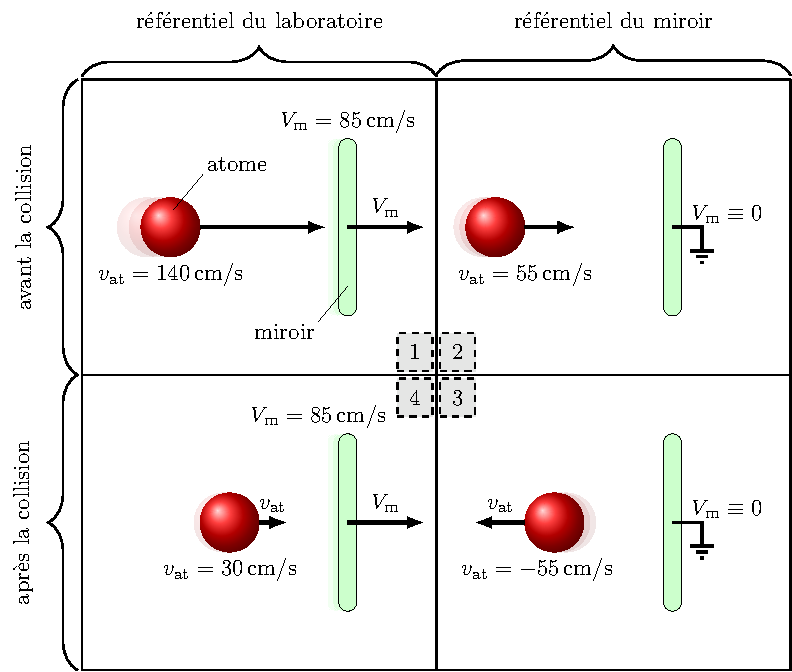
\includegraphics{P2/MiroirChoc1Atome}
\CaptionTocCaptionFig{Principe de la technique du ralentissement grâce à un miroir mobile}{ Principe de la technique du ralentissement grâce à un miroir mobile. Cette figure se lit dans le sens des aiguilles d'une montre en partant du cadran 1. Rappelons que la vitesse du \mimo est constante (voir remarque \vpageref{Rq:VitesseMiMoCste}).
\RemonteUnPeuFig
\vtop{\linewidth=\CaptionWidth %
\begin{description}
%
	\item[Cadran 1:] dans le \reflab, juste \emph{avant} la collision, la particule possède initialement une vitesse $\vatini \equiv v(t < \tcol)$ supérieure à la vitesse $\Vmir$ de la barrière. 
%	
	\item[Cadran 2:] dans le \refmir, juste \emph{avant} la collision, la particule possède une vitesse $\vatini-\Vmir$ > 0.
%	
	\item[Cadran 3:] dans le \refmir, juste \emph{après} la collision, qui se produit au temps $\tcol$, la particule possède une vitesse 
	$ - \left( \vatini-\Vmir \right) < 0$. La particule a été réfléchie.
%	
	\item[Cadran 4:] en nous replaçant dans le \reflab, juste \emph{après} la collision, nous calculons simplement la vitesse de la particule comme étant $ - \left( \vatini-\Vmir \right) + \Vmir$, soit :
\end{description}
	\[
	v_f \equiv v(t>\tcol) = 2 \Vmir - \vatini
	\pointformule
	\]
\RemonteUnPeuFig
\RemonteUnPeuFig
\RemonteUnPeuFig
\ApplicationNumerique{%
Pour des conditions typiques de nos expériences, il est ainsi possible de ralentir un atome de \cmps{140} à \cmps{30} grâce à un \mimo ayant une vitesse de \cmps{85}. L'énergie cinétique longitudinale de la particule a donc été réduite de $95\%$ (voir la section~\nref{sec:ResultatPaquetUnique}).}
}}
\label{fig:MiroirChoc1Atome}
\efigh

\subsubsection{Modélisation d'un \pat}

Pour un \pat dont l'extension longitudinale moyenne au moment de la collision est $\Delta_z$, l'instant $\tcol$ est différent pour chaque atome du paquet, et la réflexion s'étend donc sur un laps de temps de l'ordre de $\Tcol \equiv \tfrac{\Delta_z}{\MoyenneBraKet{\vatini}-\Vmir}$.
\nome{\Tcol}{Durée typique de la collision d'un \p avec le \mimo}%
%
  
Une description rigoureuse de la dynamique d'évolution  du \pat lors de sa réflexion devrait faire intervenir l'effet éventuel des collisions entre atomes. Nous pouvons cependant les négliger à partir du moment où $\Tcol$ est petit devant le temps moyen entre deux collisions inter-atomiques. Dans nos expériences cette hypothèse est bien vérifiée%
%\footnote{La densité des \pats dont il est question dans cette partie est effectivement assez faible pour pouvoir négliger les collisions durant la réflexion.}%
.

\`A l'instant $t=0$, le nuage est modélisé par une distribution spatiale ponctuelle, mais gaussienne en vitesse, \cad que la taille initiale du \pat est négligée. Cette modélisation n'a de sens que si la \dispvitlong conduit à un étalement du nuage au moment de la collision jusqu'à une taille grande devant la taille initiale réelle du \pat. Nous verrons plus loin que cette hypothèse est expérimentalement raisonnable (voir la section~\nref{sec:ResultatPaquetUnique}). Nous considérons donc la \fdd initiale dans l'\edpup:

\begin{equation}
	f_i(z,v) \equiv C \Expo{-\frac{m}{2\,\kb\,\Tlongini} 
	\left( v - \vinj \right)^2} \times \Dirac{z}
	\virguleformule
	\label{eq:fiPaquet}
\end{equation}
où $\vinj$ est la vitesse moyenne du \pat au moment de l'injection dans le \gm et $C$ est une constante de normalisation.
\nome{\vinj}{Vitesse moyenne du \pat au moment de l'injection}%
%


\subsection{Réflexion d'un \pat}
\subsubsection{Propagation libre du \pat}
Dès l'injection du \pat dans le \gm, la \dispvitlong conduit à un étalement du paquet. Nous faisons l'hypothèse que les atomes du paquet n'interagissent pas entre eux. Par suite, chaque atome se propage librement à vitesse constante et nous pouvons alors facilement écrire la \fdd du \pat à chaque instant avant la collision:
\begin{align}
	f(z,v,t) 
	&= 
%	\Integrale{
%	\Integrale{
\iint {{
	f_i(z_0,\vini)\,\Dirac{z - (z_0 + \vini t)}\,\Dirac{\vini - v}
	}{\ddint \vini}}{\ddint z_0} \nonumber \\
	&=
%	\Integrale{
%	\Integrale{
\iint {{
	C\,\Expo{-\frac{m}{2\,\kb\,\Tlongini} \,
	\left( \vini - \vinj \right)^2}\,\Dirac{z_0}\,\Dirac{z - (z_0 + \vini\,t)}\,\Dirac{\vini - v}
	}{\ddint \vini}}{\ddint z_0}
	\virguleformule
\end{align}
où l'on reconnaît, dans les fonctions $\Dirac{}$ de Dirac, la traduction d'un mouvement rectiligne uniforme.
%
\Resultat{
Nous obtenons donc l'expression de la \fdd du nuage (initialement ponctuel) dans le \gm avant la collision avec le \mimo:
\begin{equation}
	f(z,v,t) = C\,\Expo{-\frac{m}{2\,\kb\,\Tlongini} 
	\left( v - \vinj \right)^2}\,\Dirac{z - v\,t}
	\virguleformule
	\label{eq:ftPaquetAvantCol}
\end{equation}
\finformule
}
L'expression~\nref{eq:ftPaquetAvantCol} s'interprète de la manière suivante: 
\begin{itemize}
	\item on retrouve bien la même distribution en vitesse puisque le \pat se propage librement (c'est la distribution gaussienne),
	\item mais le terme $\Dirac{z - v\,t}$ traduit mathématiquement les corrélations position-vitesse qui se développent au cours de la propagation. Les atomes \sotosay{rapides} se retrouvent \sotosay{à l'avant} du nuage (\cad vers les $z$ élevés), alors que les atomes \sotosay{lents} restent à \sotosay{l'arrière} du nuage (vers les $z$ faibles).
\end{itemize}

\Resultat{
La \dat linéique $n(z,t)$ se déduit par une intégration sur la variable de vitesse $v$:
\begin{equation}
	n(z,t) \equiv \Integrale{f(z,u,t)}{\ddint u} 
	= C \, \Expo{-\frac{m}{2 \, \kb \, \Tlongini} 
	\, \left( \dfrac{z}{t} - \vinj \right)^2}
	\pointformule
	\label{eq:ntPaquetAvantCol}
\end{equation}%
\finformule
}


\casse


\subsubsection{Réflexion du \pat}\label{sec:ftPaquetReflechi}

Pour chacun des atomes d'un paquet décrit par la distribution~\nref{eq:fiPaquet}, l'instant $\tcol$ de la collision avec le \mimo correspond au temps qu'il a fallu pour que cet atome (dont la vitesse initiale est $\vini$) \sotosay{rattrape} le miroir, qui à l'instant $t=0$ se trouve en $z=\Zmirini$ et dont la vitesse est $\Vmir < \vini$:
\begin{equation}
	\tcol(\vini) = \frac{\Zmirini}{\vini - \Vmir}
	\pointformule
	\label{eq:tcol}
\end{equation}

\noindent
La figure~\nref{fig:TcolAtomeV0} représente, dans l'\edpup, les trajectoires de quelques atomes de la distribution~\nref{eq:fiPaquet}.

\bfigs
\includegraphics{P2/TcolAtomeV0}
\CaptionFigs{Représentation de la collision dans l'\edpup ($z$,$v$) pour quelques trajectoires atomiques correspondant à la distribution~\nref{eq:fiPaquet}. \\
À l'instant initial, tous les atomes sont en $z=0$, mais ont des vitesses initiales $\vini$ différentes. Les lignes pointillées représentent la vitesse $\Vmir$ et la position initiale est $\Zmirini$ du \mimo. La courbe hyperbolique représente les points de l'\edp où un atome de vitesse initiale $\vini$ rencontre le miroir. \\
Les cercles représentent quelques atomes à l'instant initial, à un instant \emph{avant} la collision du \pat, puis \emph{après} la collision.\\
$\Delta v$ désigne la dispersion de vitesse pour les trois atomes considérés dans cet exemple. La vitesse d'un atome après réflexion est symétrique de sa vitesse initiale par rapport à $\Vmir$. Ainsi, on constate que la réflexion, tout en ralentissant le paquet, conserve la dispersion de vitesses $\Delta v$, contrairement à l'effet d'une pente.}
\label{fig:TcolAtomeV0}
\efig

\noindent
Ainsi, en tenant compte de l'équation~\nref{eq:Vreflexion}, la vitesse au cours du temps $\vat(t)$ de cet atome s'écrit
\begin{equation}
	\vat(t; \vini) = 
	%\ArriveeHiglightColorMath{blue}
	{\vini\,\Heaviside{\tcol(\vini)-t}}
	+ 
	%\ArriveeHiglightColorMath{red}
	{(2\, \Vmir - \vini) \Heaviside{t-\tcol(\vini)}}
	\virguleformule
	\label{eq:vtAtomeReflexion}
\end{equation}
où les vitesses de la particule %\DepartHighlightColor{blue}
{avant} et %\DepartHighlightColor{red}
{après} la collision apparaissent clairement, $\Heaviside{}$ est la \termetech{fonction de Heaviside}. 
Aussi, nous connaissons la position $\zat(t)$ de cet atome en intégrant l'équation~\nref{eq:vtAtomeReflexion}:
%\MakeFlecheHighlightColor{blue}%
%\MakeFlecheHighlightColor{red}%
\begin{equation}
	\zat(t; \vini) \equiv \IntegraleBornes{\vat(t'; \vini)}{\ddint t'}{0}{t} = \vini t - 2\,(\vini-\Vmir)\,(t-\tcol(\vini)) \Heaviside{t-\tcol(\vini)}
	\pointformule
	\label{eq:ztAtomeReflexion}
\end{equation}
L'évolution de la fonction de distribution du \pat s'établit en utilisant les équations~\nref{eq:fiPaquet} et~\nref{eq:tcol} à~\nref{eq:ztAtomeReflexion}. 
%
\EnFaitNon
{

\begin{align}
	f(z,v,t) 
	=& 
	\iint
	%\DepartHighlightColorMath{blue}
	{
	f_i(z_0,\vini)
	}	
	%\DepartHighlightColorMath{red}
	{
	\Dirac{z - \zat(t)}
	}	
	%\DepartHighlightColorMath{green}
	{
	\Dirac{v - \vat(t)}
	}
	\ddint \vini \ddint z_0 \nonumber\\
	=& 
	\iint
	%\ArriveeHiglightColorMath{blue}
	{
	C \Expo{-\frac{m}{2\,\kb\,\Tlongini} 
	\left( \vini - \vinj \right)^2}\Dirac{z_0}
	}
	\nonumber\\
%%%%%%%%%%%%%%%%%%%%%%%%%%%%%%%%%%%%%%%%%%%%%%%%%%%%%%%%%%%%%%%%%%%%%%%%%%%%%%%%%%%%%%%%%%%%%%%%%%%%%%%%%%%%%%%%%%%%%%%%%%%%%%%%%%%%%%%%
	&	\;\;\;\;\;\;\;\;\;\; 
	%\ArriveeHiglightColorMath{red}
	{\DIRAC{z - \left( \vini t - 2(\vini-\Vmir)\left(t - \frac{\Zmirini}{\vini - \Vmir}\right) \Heaviside{t -  \frac{\Zmirini}{\vini - \Vmir}} \right)} 
	}
	\nonumber\\
%%%%%%%%%%%%%%%%%%%%%%%%%%%%%%%%%%%%%%%%%%%%%%%%%%%%%%%%%%%%%%%%%%%%%%%%%%%%%%%%%%%%%%%%%%%%%%%%%%%%%%%%%%%%%%%%%%%%%%%%%%%%%%%%%%%%%%%%
	&	\;\;\;\;\;\;\;\;\;\; 
	%\ArriveeHiglightColorMath{green}
	{\DIRAC{v - \left( \vini \Heaviside{\frac{\Zmirini}{\vini - \Vmir} - t} + (2 \Vmir - \vini) \Heaviside{t - \frac{\Zmirini}{\vini - \Vmir}} \right)}
	}
	\nonumber\\
	&	\;\;\;\;\;\;\;\;\;\; \ddint \vini \ddint z_0
	\pointformule
	\label{eq:ftPaquet}
\end{align}
%\MakeFlecheHighlightColor{blue}\MakeFlecheHighlightColor{red}\MakeFlecheHighlightColor{green}
%Dans cette égalité, les différents termes de l'intégrale sont repérés par des couleurs lors de leur développement. 
On note que l'intégration suivant la variable $z_0$ est immédiate du fait de la présence du terme $\Dirac{z_0}$, et nous effectuons le remplacement directement.
Cette équation~\nref{eq:ftPaquet} ne semble pas simple à intégrer dans la mesure où les termes de Dirac contiennent des fonctions de Heaviside et que la vitesse $\vini$ y apparaît plusieurs fois, notamment au dénominateur. 

En revanche, on remarque que la condition sur le temps $t$ pour qu'un atome ayant une vitesse initiale $\vini$ donnée ait subi la collision avec le \mimo et qui s'écrit:
\[
	t \geq \tcol(\vini) = \frac{\Zmirini}{\vini - \Vmir} 
	\virguleformule
\]
peut se traduire (d'après l'équation~\nref{eq:tcol}) de manière équivalente en une condition sur la vitesse initiale $\vini$ d'un atome, traduisant le fait que ce dernier \emph{aura} subi la collision à un temps $t$ donné:
\begin{equation}
	\vini \geq \vinicol(t) \equiv \Vmir + \frac{\Zmirini}{t} 
	\pointformule
	\label{eq:vinicolt}
\end{equation}
$\vinicol(t)$ est, pour ainsi dire, \sotosay{la vitesse initiale dont un atome a besoin afin de subir une collision à l'instant $t$ choisi}.


Grâce à cette formulation, on peut ré-écrire l'argument des fonctions de Heaviside des équations~\nref{eq:vtAtomeReflexion} et~\nref{eq:ztAtomeReflexion} de manière à exprimer l'équation~\nref{eq:ftPaquet} sous la forme:
\begin{align}
	f(z,v,t)
	=&
	\int
%%%%%%%%%%%%%%%%%%%%%%%%%%%%%%%%%%%%%%%%%%%%%%%%%%%%%%%%%%%%%%%%%%%%%%%%%%%%%%%%%%%%%%%%%%%%%%%%%%%%%%%%%%%%%%%%%%%%%%%%%%%%%%%%%%%%%%%%
	%\ArriveeHiglightColorMath{blue}
	{
	C \Expo{-\frac{m}{2\,\kb\,\Tlongini} 
	\left( \vini - \vinj \right)^2}
	}
	\nonumber\\	%%%%%%%%%%%%%%%%%%%%%%%%%%%%%%%%%%%%%%%%%%%%%%%%%%%%%%%%%%%%%%%%%%%%%%%%%%%%%%%%%%%%%%%%%%%%%%%%%%%%%%%%%%%%%%%%%%%%%%%%%%%%%%%%%%%%%%%%
	&	\;\;\;\;\; 
	%\ArriveeHiglightColorMath{red}
	{\DIRAC{z - \vini t + 2(\vini-\Vmir)\left(t - \frac{\Zmirini}{\vini - \Vmir}\right) \Heaviside{\vini - \vinicol(t)} }
	}
	\nonumber\\
%%%%%%%%%%%%%%%%%%%%%%%%%%%%%%%%%%%%%%%%%%%%%%%%%%%%%%%%%%%%%%%%%%%%%%%%%%%%%%%%%%%%%%%%%%%%%%%%%%%%%%%%%%%%%%%%%%%%%%%%%%%%%%%%%%%%%%%%
	&	\;\;\;\;\;
	%\ArriveeHiglightColorMath{green}
	{\DIRAC{v - \vini \Heaviside{\vinicol(t) - \vini} - (2 \Vmir - \vini) \Heaviside{\vini - \vinicol(t)}}
	}
	\nonumber\\
	&	\;\;\;\;\; \ddint \vini \nonumber
	\virguleformule
\end{align}
qui se coupe naturellement en deux en intégrant de $-\infty$ à $\vinicol(t)$, puis de $\vinicol(t)$ à $+\infty$. Ceci simplifie les fonctions de Heaviside qui valent sur ces domaines soit $0$, soit $1$:
\begin{align}
	f(z,v,t)	=&
	\IntegraleBornes{
	C \Expo{-\frac{m}{2\,\kb\,\Tlongini} \left( \vini - \vinj \right)^2}
	\Dirac{z - \vini t}
	\Dirac{v - \vini}
%	}
	}{\ddint \vini}{-\infty}{\vinicol(t)} \nonumber \\
	+&\IntegraleBornes{
	C \Expo{-\frac{m}{2\,\kb\,\Tlongini} \left( \vini - \vinj \right)^2}
	\Dirac{z - t( 2\Vmir-\vini) - 2 \Zmirini}
	\Dirac{\vini + v - 2 \Vmir}
%	}
	}{\ddint \vini}{\vinicol(t)}{+\infty} \nonumber
	\virguleformule
%	\label{eq:ftPaquetSimple}
\end{align}

}
%
%\Resultat
{
%En conclusion, nous pouvons établir 
On peut ainsi calculer
la \fdd d'un \pat initialement ponctuel de \templong $\Tlongini$ injecté à l'instant initial à une vitesse moyenne $\vinj$ en direction d'une barrière infinie de potentiel ayant une vitesse $\Vmir$ et une avance $\Zmirini$ à l'instant initial:
\begin{align}
	f(z,v,t)	=&%
	C \Expo{-\frac{m}{2\,\kb\,\Tlongini} \left( v - \vinj \right)^2}
	\Dirac{v - \frac{z}{t}}
	\Heaviside{\Vmir + \frac{\Zmirini}{t} - v}	\nonumber \\
	+&%
	C \Expo{-\frac{m}{2\,\kb\,\Tlongini} \left( v - 2 \Vmir + \vinj \right)^2}
	\Dirac{v - \frac{z-2\Zmirini}{t}}
	\Heaviside{\Vmir - \frac{\Zmirini}{t} - v}
	\pointformule
	\label{eq:ftPaquetResultat}
\end{align}
On distingue bien ici les deux termes correspondant:
\begin{itemizel}
	\item au nuage initialement injecté dans le guide magnétique (voir l'équation~\nref{eq:ftPaquetAvantCol}) qui intervient aux temps courts (avant la collision du nuage avec le \mimo).
	\item au nuage réfléchi, dont la vitesse moyenne est $2\,\Vmir-\vinj$ et qui intervient aux temps longs (après la collision). On remarque aussi dans ce terme, que la \templong n'a pas été modifiée lors de la collision. 
\end{itemizel}
}
Le fait de ne pas modifier la \dispvitlong du \pat est une propriété remarquable qui distingue la \techmimo par rapport à l'utilisation d'une \secpent. Ce point est discuté dans la section~\nref{sec:MiroirVioleLiouville}

%\Intuition{Une manière simple de se convaincre que les propriétés du \pat ne sont pas modifiées par la réflexion sur le \mimo peut se présenter sous cette forme, par analogie avec l'optique newtonienne:
%
%\emph{après} la collision, nous obtenons un \pat qui est tout simplement \emph{l'image} du paquet initial par réflexion dans un miroir, et dont les propriétés sont identiques. 
%}


\subsection{Évolution de la densité atomique dans le \gm}

Comme nous l'avons précisé dans le chapitre~\nref{chap:JetAtomique} (section~\nref{sec:MesureJat}), la grandeur qui nous est expérimentalement accessible par la mesure est la \datlin $n(z,t)$ dans le \gm. 
\Resultat{
Celle-ci s'obtient par intégration de l'équation~\nref{eq:ftPaquetResultat} par rapport à la variable $v$:
\begin{align}
	n(z,t) & \equiv	\Integrale{f(z,v,t)}{\ddint v} \nonumber \\
	& =C \left[ \Expo{-\frac{m}{2\,\kb\,\Tlongini} \left( \frac{z}{t} - \vinj \right)^2}
	\right.
	\nonumber \\
	& \qquad +
	\left.
	\Expo{-\frac{m}{2\,\kb\,\Tlongini} \left( \frac{z-2\Zmirini}{t} - 2 \Vmir + \vinj \right)^2} \right] \Heaviside{t\,\Vmir + \Zmirini - z}
	\pointformule
	\label{eq:NtPaquetResultat}
\end{align}
\finformule
}

\casse

\noindent
L'expression~\nref{eq:NtPaquetResultat} s'interprète en remarquant que La \dat est donnée par la somme des contributions de deux nuages se propageant en sens inverse:
\begin{itemize}
	\item le premier terme de la somme entre parenthèses correspond au nuage initial lancé dans le guide.
	\item le second terme correspond au nuage symétrique du premier par rapport au \mimo dont l'équation du mouvement est $\Zmirini + \Vmir\,t$.
	\item le terme $\Heaviside{\cdots}$ de Heaviside traduit mathématiquement le fait qu'aucun atome n'est en fait passé de l'autre coté du \mimo ($z > \Zmirini + t\,\Vmir$).
\end{itemize}


\noindent
La figure~\nref{fig:NtPaquetResultat} donne une représentation de l'expression~\nref{eq:NtPaquetResultat} en fonction de $z$ à des instants $t$ caractéristiques: \emph{avant}, \emph{pendant}, et \emph{après} la collision du \pat avec le \mimo.%

\bfigs
%
\ifthenelse{\NoAnimationsInFigures > 0}{%
\includegraphics{P2/NtPaquetResultatAnimate_1}%
}{%
\animategraphics[poster=last]{10}{images/P2/NtPaquetResultatAnimate}{}{}%
}
\CaptionFigs{\AnimateOnline Représentation de la \datlin $n(z,t)$ donnée par l'expression~\nref{eq:NtPaquetResultat} en fonction de $z$ pour différents instants : (a) avant, (b) pendant, et (c) après la collision.}
\label{fig:NtPaquetResultat}
\efig

%
%\subsection{Réflexion élastique sur une barrière harmonique en mouvement}\label{sec:BarriereHarmonique}
%L'étude d'une barrière de potentiel non-infini, \cad qui ne se comporte pas comme un miroir vis a vis des atomes est plus délicate. En effet, la relation~\nref{eq:Vreflexion} reste valable, mais l'équation~\nref{eq:vtAtomeReflexion} n'est plus juste dans la mesure où les atomes ne rebondissent plus instantanément. Le temps qu'un atome va mettre à être réfléchi (au sens de l'équation~\nref{eq:Vreflexion}) va en général dépendre de sa vitesse. 
%Il existe cependant une autre forme de potentiel qui donne un résultat simple: Un potentiel en forme de demi-parabole. En rencontrant un tel potentiel, toutes les particules mettent le même temps à être réfléchies puisque la (demi-)période d'oscillation est indépendante de la vitesse d'arrivée des atomes. Ainsi, tout ce passe avec une barrière à forme harmonique comme avec une barrière infinie, mais avec un décalage temporel d'une demi-période d'oscillation.


\section{Mise en \oe uvre expérimentale}\label{sec:MiroirMiseEnOeuvre}

%Comme évoquer plus haut, cette méthode repose sur l'utilisation d'un potentiel dépendant du temps, prenant la forme ici d'un \mimo. Il existe différentes manières expérimentales pour mettre en \oe uvre cette technique.
%Certaines équipe utilise des courant alternés dans des bobine afin de mettre en mouvement des atomes. da.................

\subsection{Un \mima à aimants permanents}

\subsubsection{Différentes manières de réfléchir des atomes}
La réflexion d'atomes sur \mimo a déjà été étudiée dans le contexte des atomes ultra-froids. L'utilisation d'ondes lumineuses évanescentes se propageant à la surface d'un prisme, et dont l'intensité était modulée dans le temps, permit la manipulation d'atomes pour l'optique atomique: focalisation de trajectoires atomiques, formation d'images multiples d'un point source et modulation de la phase d'onde de De Broglie~\cite{SSD95,ASD96}.

La mise en \oe uvre d'un \mima repose sur l'interaction Zeeman entre un \chm inhomogène et le moment dipolaire magnétique des atomes. 
Des miroirs magnétiques pour l'optique atomique ont été réalisés de manières variées, en utilisant des arrangements d'aimants permanents~\cite{SMR96}, des micro-électro-aimants~\cite{JDT98, DZL99}, ou encore divers supports magnétiques (tels que de des disquettes informatiques~\cite{HBR97}, des bandes vidéo~\cite{RHH00}).  
%L'équipe de Tilma Esslinger en Allemagne a montré qu'il était possible de manipuler, sur ce principe, des ondes cohérentes de matières (extraites d'un \bec d'atome de \Rb)~\cite{BKG01}.

\casse

\subsubsection{Produire une \bapot dans le \gm}

Nous allons maintenant nous intéresser à la réalisation expérimentale d'une barrière de potentiel magnétique sur l'axe $z$ de notre guide. La mise en mouvement de cette barrière sera traitée dans la \autoref{sec:MiroirMiseEnMouvement}.

%Dans le \gm de notre \setup, les atomes se propagent librement suivant la direction $z$. 
%La réalisation d'un \mima suivant l'axe de propagation des atomes repose sur le fait que, dans nos conditions expérimentales, le potentiel effectivement ressenti par les atomes est proportionnel au module du \chm\footnote{Le potentiel ressenti par les atomes est proportionnel au module du \chm seulement dans l'hypothèse d'une évolution adiabatique des atomes au sein du \chm, \cad que les moments magnétiques des atomes doivent rester alignés avec les ligne de champ. Cette hypothèse est valide pour toute nos expériences.} et dépend donc de la composante longitudinale du \chm. 
Nous avons choisi d'utiliser des aimants permanents afin de moduler la valeur du \chm longitudinal $\Bpara\,\Vecteur{e_z}$ sur l'axe du guide. En effet, nous avons vu dans la section~\nref{sec:ConfigMagnetiqueGuide} que le potentiel auquel sont soumis les atomes dans le guide dépend, entre autres choses, de la composante longitudinale du \chm. Ainsi, une valeur localement élevée du champ $\Bpara$ va avoir pour effet de repousser les atomes de \Rb préparés dans l'état $\EtatSFmF{1}{-1}$.
Nous pourrons donc réflechir un atome dans le guide si la \bapot magnétique possède une hauteur suffisante (\cad supérieure à l'énergie cinétique longitudinale de l'atome).

\EnFaitNon{
Le \chm longitudinal dont il est question ici peut etre produit de différentes manières:
\begin{itemize}
	\item Bobine suivant l'axe du \gm: Cette technique est simple à mettre en \oe uvre mais la mise en mouvement d'une bobine enroulée autour du guide parait délicate, notamment s'il s'agit de faire se mouvoir ce montage de manière répétée.
	\item Paire de bobines placées de part et d'autre du guide:] Ceci rappelle la configuration utilisée pour l'évaporation du \jat sur une céramique du chapitre~\nref{chap:Ceramique} dans leque les bobines étaient placées en configuration Helmholtz, produisant un fort champ transverse. Afin de créer un champ longitudinal sur l'axe du \gm, les bobines doivent être placées en configuration anti-Helmholtz. Le champs transverses des deux bobines s'annulent ainsi sur l'axe du guide. 
	\item Paire d'aimants permanents: Encore en rapport avec le chapitre mentionné précedemment dans lequel nous avons utilisé une paire d'aimants permanent créant un fort \chm transverse. Cette fois-ci, les aimants sont placés en vis-à-vis avec des aimentations opposées de manière à produire un champ longitudinal sur l'axe du \gm. 
\end{itemize}

C'est cette dernière solution qui à été retenue car elle ne nécessite pas d'apport de courant et se présente sous la forme d'un montage léger et facile à mettre en mouvement. 
}


\subsection{Disposition des aimants autour du \gm}
%Nous décrivons ici la configuration géométrique utilisée pour le positionnement des aimants.

%\Remarque
{
\subsubsection{Disposition symétrique des aimants}
Si nous désirons moduler spatialement la composante longitudinale $\Bpara$ du \chm sur l'axe du guide, il est en revanche très important de ne pas générer de composantes transverses. En effet, nous avons vu au chapitre~\nref{chap:Ceramique} que moduler le champ transverse a pour effet de dévier latéralement la trajectoire des atomes. Ceci conduit à une élimination de certains atomes si cette déviation se fait au niveau d'une pièce en céramique (voir la \autoref{sec:ResultatVariationFlux}).

Afin de ne pas avoir de composantes transverses du \chm au niveau de l'axe du guide, celui-ci doit être un \emph{axe de symétrie} pour l'alimentation, \cad qu'il faudra disposer les aimants de manière symétrique par rapport au guide, avec leur aimantation deux à deux opposées. Dans notre cas, l'aimantation de chaque aimant pointe vers le guide.
La configuration choisie ainsi que l'allure de la \bapot produite suivant l'axe du \gm sont représentées sur la figure \ref{fig:AimantPaireChampLong}.
}
\bfighs
\subfloat[]{\includegraphics{P2/AimantPaireChampLong}}
\subfloat[]{\includegraphics{P2/AimantPaireChampLongAxe}}
\CaptionFigs{
(a): disposition des aimants autour de l'axe $z$ du \gm et représentation de quelques lignes de \chm des aimants. Une configuration symétrique de l'aimantation par rapport à l'axe $z$ permet de produire un champ purement longitudinal sur cet axe. L'espacement entre les aimants est d'environ \cm{5}.
(b): allure du module du \chm sur l'axe $z$ du guide. Pour des atomes préparés dans l'état $\EtatSFmF{1}{-1}$, cela correspond à une \bapot dont la hauteur est déterminée par la valeur maximale $\Bparamir$. L'extension longitudinale de cette barrière est d'environ \cm{5}.
}
\label{fig:AimantPaireChampLong}
\efigh

\casse

Les aimants utilisés sont les mêmes que ceux qui ont servi pour l'évaporation sur une céramique (chapitre~\nref{chap:Ceramique}) et sont décrits dans l'annexe~\nref{annexe:ModelisationAimants}.
Ils sont placés sur un support en polystyrène %
\footnote{L'utilisation d'un matériau léger pour confectionner le support du \mimo est justifiée dans la \autoref{sec:MiroirMiseEnMouvement}.} %
ayant la forme d'un \enquote{U}.
La figure~\nref{fig:MiroirMontageAimant} représente ce montage et le positionnement de celui-ci autour du \gm. 
\bfighs
\subfloat[]{\includegraphics{P2/MiroirMontageAimant}}\quad
\subfloat[]{\includegraphics[height = 7cm]{P2/MiroirMontageAimantPhoto}}
\CaptionFigs{(a): Vue schématique en coupe du \mima en place autour du guide. L'utilisation de plusieurs aimants de chaque côté permet de créer des \chms plus importants et donc d'augmenter la hauteur de la \bapot. Avec quatre aimants de chaque coté du guide, nous disposons d'une \bapot d'une hauteur $\mu \, \Bparamir$ avec $\Bparamir \equiv \max({B_0}(z)) = \gauss{160}$. (b): photographie du montage. Les aimants sont fixés sur un support en polystyrène.}
\label{fig:MiroirMontageAimant}
\efigh


\subsection{Potentiel \sotosay{ressenti} par les atomes dans le \gm}\label{sec:MiroirPotentielRessenti}
Intéressons nous plus précisément au potentiel auquel sont soumis les atomes dans le \gm.
Rappelons que l'équation~\nref{eq:PotentielTubesHyp} montre la dépendance du potentiel de piégeage en fonction de la composante longitudinale $B_0\,\Vecteur{e_z}$ du \chm le long de l'axe du guide. 
Cette dépendance est ici mise à profit afin de produire la réflexion des atomes grâce à une modulation spatiale du \chm longitudinal ${B_0}(z)\,\Vecteur{e_z}$.


La superposition du champ transverse fourni par le guide et du champ longitudinal produit par le \mima nous permet de déduire le potentiel auquel sont soumis les atomes%
\footnote{Un \chm de la forme $\Vecteur{B}={B_0}(z)\,\Vecteur{e_z}$ ne vérifie évidemment pas les équations de Maxwell puisqu'il n'est pas de divergence nulle. Néanmoins, les gradients transverses de \chm mis en jeu par le \mima sont très faibles (typiquement quelques dizaine de \gausspcm{}) en comparaison du gradient produit par le \gm (de l'ordre de \gausspcm{500}). On peut donc considérer raisonnablement que le potentiel auquel sont soumis les atomes est bien celui donné par la formule~\nref{eq:MiroirUB0}.}%
:

\begin{equation}
	U(r,z) = \mu\,\Module{\Vecteur{B}} = \mu\,\sqrt{\gradB^2\,r^2 + {{\Bpara}(z)}^2}
	\pointformule
	\label{eq:MiroirUB0}
\end{equation}

\ApplicationNumeriqueTitre{Hauteur de la \bapot sur l'axe du guide}{
Calculons la hauteur de la \bapot qui résulte de la mise en place du \mima sachant que:
\begin{itemize}
	\item le \mima produit sur l'axe du guide un champ longitudinal dont la valeur maximale est $\Bparamir=\gauss{160}$.
	\item les atomes de \Rb sont piégés dans l'état $\EtatSFmF{1}{-1}$ dont le moment magnétique est $\mu = \tfrac{\muB}{2} \approx \SI{4.6E{-24}}{\square\meter\ampere}$.
\end{itemize}
Nous déduisons que, pour qu'un atome soit réfléchi par cette \bapot magnétique,  la vitesse relative maximale $\vmax$ de l'atome par rapport au miroir est donnée par:
\[ 
	\frac{1}{2}\,m\,\vmax^2 = \mu\,\Bparamir 
	\virguleformule
\]
qui correspond ici à:
\[
	\vmax = \SI{1}{\meter\per\second}
	\pointformule
\]
\finformule
}%
\nomeRemonte{\vmax}{Vitesse maximale relative à la \bapot pour qu'un atome soit réfléchi}{3cm}%

%\RemarqueTitre
\subsubsection{Caractère tridimensionnel du mouvement}{
%\inlinefig{\includegraphics[height=3cm]{P1/TrajGuide_a}}
Il est important de garder à l'esprit que les atomes ne se propagent pas \emph{exactement} suivant l'axe $z$. Ils sont aussi animés d'un mouvement dans le plan transverse $(x,y)$ (voir la section~\nref{sec:MesureTempTrans}). Or nous avons vu dans la section~\nref{sec:ConfigMagnetiqueGuide} que plus la composante longitudinale $\Bpara$ est importante, plus le piège s'ouvre transversalement.
Réciproquement, plus un atome \sotosay{orbite} loin de l'axe du guide, moins il est sensible à la présence du \mima. 
%Pour s'en convaincre, il suffit de dériver le potentiel $U(r,z)$ par rapport à $z$.
% et de constater que c'est une fonction dont le module est décroissant en $r$..
%Ceci est dû au fait que le module du \chm donné par l'équation~\nref{eq:MiroirUB0} est d'autant plus sensible à la composante longitudinale ${B_0}(z)$, que la composante transverse $\gradB^2\,r^2$ est petite.
%\[
%\Diff{U(r,z)}{z} =\mu\,\Diff{\Bpara(z)}{z}\,\frac{1}{\sqrt{1+\tfrac{\gradB^2\,r^2}{\Bpara^2}}}
%\]

Il en résulte un couplage entre le mouvement transverse des atomes et le mouvement longitudinal suivant l'axe du guide.
Nous allons cependant négliger cet effet et considérer que la modélisation \emph{unidimensionnelle} est correcte.
Nous justifions ce choix par le fait que:
\begin{itemize}
	\item les fréquences d'oscillations transverses dans le \gm sont de l'ordre du kilohertz.
	\item le temps que met un atome à être réfléchi est typiquement d'un dixième de seconde (déduit de l'extension longitudinale de la barrière, $\approx \cm{6}$, et de vitesses relatives inférieures à $\vmax = \SI{1}{\meter\per\second}$).
\end{itemize} 
Les deux échelles de temps étant très différentes, il est raisonnable de négliger le couplage entre degrés de liberté transverses et longitudinal.
% (C'est une \emph{approximation séculaire}).
}

\NoteGael{PEUT ETRE FIGURE 3D\\
La figure~\nref{fig:PotentielGuideB0} montre la déformation du potentiel auquel les atomes sont soumis dans le \gm en présence du \mima.
%\bfig
%\includegraphics[width = \linewidth]{P2/PotentielGuideB0}
%\CaptionFig{fig:PotentielGuideB0}
%\label{fig:PotentielGuideB0}
%\efig
}

\vspace{5cm}

\casse

\section{Mise en mouvement du miroir} \label{sec:MiroirMiseEnMouvement}

Afin de mettre en mouvement le \mima%représenté sur la figure~\nref{fig:MiroirMontageAimant}
, nous l'avons fixé sur un \sotosay{tapis roulant} longeant le \gm. Dans la suite, ce système sera désigné par le terme \sotosay{\conv}.  Une représentation du système fait l'objet des figures~\nref{fig:MiroirConveyerSchema} et~\nref{fig:MiroirConveyerPhoto}.

\bfig
\includegraphics{P2/MiroirConveyer}
\CaptionFig{Schéma représentant le \setup du \mimamo. Celui-ci est fixé à la courroie du \conv et parcourt le rail de manière cyclique à la vitesse $\Vmir$. À chaque extrémité il subit une phase de retournement hémicirculaire. \\
Une fois injecté dans le \gm, le \pat issu du \pmo (PMO) atteint la région couverte par le \conv.  \\
Un laser sonde positionné en $z=\zsonde$ permet de mesurer la \datlin (voir la section~\nref{sec:MesureDensiteGuide}).
%En pratique, le \pmo (PMO) est protégé de par un bouclier en $\mu$-métal contre l'influence du miroir magnétique.
}
\label{fig:MiroirConveyerSchema}
\efig
\bfig
\includegraphics[width = \linewidth]{P2/MontageMiroirConveyer}
\CaptionFig{Photographie du \setup. On y distingue le \gm dans le tube de verre et le \mimo fixé sur le \conv.}
\label{fig:MiroirConveyerPhoto}
\efig

\RemarqueTitre{Accélération violente en bout de rail}{
Le fonctionnement cyclique du \conv implique que le \mimo fixé à la courroie doit subir à chaque extrémité du rail une phase de retournement hémicirculaire. 
On notera que cette accélération en bout de rail n'est pas purement centrifuge. En effet, le miroir doit résister non-seulement à une force centrifuge qui tend à l'arrachement radial du miroir, mais aussi à une force de cisaillement qui tend à faire plier le miroir autour de l'axe de rotation. 

Cette deuxième composante vient tout simplement du fait que :
\begin{itemize}
	\item sur la partie rectiligne du \conv, chaque point du miroir possède la même vitesse (celle de la courroie), 
	\item lors de la phase circulaire, les points du miroir situés loin de l'axe de rotation doivent posséder une vitesse plus importante.
\end{itemize}

En d'autres termes, cela traduit la \emph{mise en rotation} du miroir à l'instant \emph{précis} où celui-ci passe de la partie rectiligne à la partie circulaire. Cette accélération est très violente, elle est même théoriquement infinie si l'on devait considérer le système comme étant rigide. En pratique, la courroie absorbe le choc en se déformant, mais il est prudent d'assurer une bonne rigidité de fixation des aimants tout en maintenant la légèreté de l'ensemble afin d'en minimiser le moment d'inertie.
}

\subsection{Le \conv}

Le \conv a été acheté auprès de la société NORCAN. La longueur du rail est de $\cm{120}$, et la courroie de $\cm{250}$ de long qui est enroulée autour, comporte 50 emplacements de fixation (tous les \cm{5}). Le moteur électrique monté d'origine sur le système est de type asynchrone triphasé et est refroidi par un ventilateur dont l'axe est solidaire de l'arbre moteur. Il est par ailleurs contrôlé par un boîtier électronique externe fournissant le courant alternatif à la fréquence voulue, et sur lequel peuvent être programmés les différents paramètres liés au mouvement du \conv:
\begin{itemize}
	\item tension efficace appliquée au moteur,
	\item accélération au démarrage et au freinage,
	\item vitesse maximale, etc...
\end{itemize}

La liaison cinématique entre l'arbre moteur et le \conv est effectuée par un étage de démultiplication à vis sans fin de rapport $\ttfrac{1}{10}$. L'ensemble moteur est monté sur \termetech{silent-bloc} afin d'éviter les contraintes mécaniques entre le \conv et le bloc moteur.

\EnFaitNon
{
\subsection{Mesure de stabilité de la vitesse du tapis}
Une connaissance précise de la vitesse du \conv est requise pour mener à bien les expériences de \mimo. 
Aucun dispositif n'étant prévu à cet effet, nous avons installé une diode électroluminescente (LED) couplée à une photodiode dans le carénage de protection du moteur, de manière à ce que le faisceau lumineux soit coupé à chaque passage d'une des 5 palles du ventilateur (solidaire de l'arbre moteur). 
Le signal \sotosay{haché} récupéré par la photodiode nous permet de déterminer la vitesse de rotation du moteur et d'en déduire la vitesse du \conv (de manière très précise du fait de l'étage de démultiplication qui joue en notre faveur).\Cahier{8,22} \Cahier{7,35}
\picskip{0}
Nous avons ainsi pu mesurer la stabilité de la vitesse du \conv dans différentes conditions, et il s'est avéré qu'avec les réglages d'origine, la vitesse du \conv n'était pas stable à faible vitesse (en dessous de $\cmps{20}$, les fluctuations relatives de vitesse atteignaient près de $50$\%)\Cahier{7,163}. 
Grâce aux différentes possibilités de réglage offertes pas le boîtier électronique du \conv, il nous a été possible d'augmenter le couple du moteur. En contrepartie d'un échauffement accru du moteur, la stabilité en vitesse du \conv est grandement améliorée puisqu'il est possible de faire fonctionner le \conv à une vitesse de $\cmps{5}$ sans à coup (fluctuations inférieures à $10$\%).
% (la dispersion de vitesse est inférieur à $\cmps{2}$).
\Cahier{7,187 peut être encore mieux avec 8,21-22 pour la figure~\nref{fig:ConvStability} aussi.}
}

{\AjouteLigne}

\subsection{Synchronisation du mouvement avec le reste de l'expérience}

%La stabilité en vitesse du \conv dont il est question plus haut nous permet de considérer sa vitesse comme constante sur toute la durée d'une expérience de réflexion d'atome. 
Il est absolument crucial pour nos expériences de disposer d'une synchronisation parfaite du \mimo avec le lancement du \pat dans le \gm. Le mouvement du \conv est difficile à contrôler de manière dynamique du fait de l'inertie du système, d'autant plus que le boîtier électronique qui le commande n'est pas prévu pour ce genre de tâche. En revanche, tout notre dispositif expérimental de production et d'injection de \pats est piloté par un ordinateur \nomofficiel{National Instruments} qui permet, entre autres choses, de déclencher les séquences expérimentales. 

Dans le but d'assurer une bonne synchronisation, nous avons placé à proximité du \conv une sonde magnétique sensible au passage du \mimo et qui déclenche l'exécution de notre séquence. Cette dernière comporte d'ailleurs un \sotosay{temps mort}(pendant lequel rien ne se passe) réglable à volonté depuis l'ordinateur et qui permet de définir l'avance $\Zmirini$ qu'a le \mimo par rapport au \pat lors de son injection dans le \gm. 


%\casse


\section{Résultats obtenus}\label{sec:Resultats}
Les expériences réalisées dans le but de démontrer l'efficacité de cette technique seront présentées selon deux aspects complémentaires:
\begin{itemizel}
	\item expériences avec des \pats uniques afin de tester les prédictions théoriques et de démontrer l'efficacité de notre méthode de ralentissement. Elles font l'objet de la sous-section~\nref{sec:ResultatPaquetUnique}.
	\item expériences avec des \patss pour étudier le problème dans le contexte plus précis de notre expérience, \cad en vue de réaliser un \jatgm lent et ultra froid. Elles font l'objet de la sous-section~\nref{sec:ResultatPaquetMultiple} et nous amèneront à considérer les avantages de la \techmimo par rapport à l'utilisation d'une \secpent.
\end{itemizel}
Pour tous les résultats présentés ci-dessous, un courant de $\SI{200}{\ampere}$ dans chaque tube du \gm a été utilisé, générant ainsi un gradient transverse de \chm $b'=\gausspcm{500}$. 

Dans toute la suite, l'origine de l'axe $z$ du \gm est prise comme étant la position initiale du \pat (qui correspond à la position du \pmo), et le temps $t=0$ est défini par l'instant où le \pat est injecté dans le \gm. 
La détection des atomes s'effectue grâce à la technique décrite dans la section~\nref{sec:MesureDensiteGuide}. Nous pouvons de cette manière accéder à la \datlin $n(z,t)$ en $z = \zsonde = \cm{175}$ (sauf mention contraire). 

\subsection{Réflexion d'un paquet unique} \label{sec:ResultatPaquetUnique}
Chaque expérience décrite dans cette sous-section consiste en l'injection à une vitesse $\vinj$ d'un seul \pat dans le \gm. On étudie le comportement de ce paquet en présence du \mimo dont la vitesse est $\Vmir < \vinj$ et sa position à l'instant initial est $\Zmirini$.

\ifthenelse{\FormatEUE > 0}{}
{\AjouteLigne}

\subsubsection{Caractérisation du \pat avant la collision}
\label{sec:CaracPatLibre}
De manière à pouvoir étudier la réflexion sur le \mimo, il nous faut d'abord caractériser le \pat avant la réflexion. 
Pour ce faire, chaque expérience impliquant le \mimo est réalisée \emph{une deuxième fois}, à l'identique, mais \emph{sans l'intervention du \mimo}. Nous obtenons de cette manière, pour chaque expérience, un signal supplémentaire de détection correspondant à la propagation libre d'un \pat. 
%
\inlinefig{{\includegraphics[scale=0.97]{P2/CourbePaquetLibre}}}%
%
De ce signal $n(\zsonde,t)$, nous déduisons les caractéristiques initiales du paquet en ajustant une fonction%
\footnote{Rappelons la formule :
$
n(\zsonde,t) = C\,\Expo{-\tfrac{m}{2\,\kb\,\Tlongini}
	\,\left( \tfrac{\zsonde}{t}-\vinj\right)^2}
$, dont les paramètres à ajuster sont la vitesse d'injection $\vinj$, la \templong $\Tlong$ ainsi que l'amplitude $C$ du signal.}
 donnée par l'équation~\nref{eq:ntPaquetAvantCol}. 
La figure ci-contre montre un exemple de signal expérimental de détection $n(\zsonde,t)$ pour un \pat typique en propagation libre. On y distingue nettement le passage du \pat devant le laser sonde, environ \seconde{1.5} après son injection. 
\picskip{3}
\noindent
En utilisant la fonction d'ajustement (dessinée en rouge), nous déduisons la vitesse d'injection $\vinj = \cmps{120}$ et la \templong $\Tlong = \microK{150}$ du \pat (cette température correspond à une \dispvitlong de \cmps{12}).
%, et pour lequel nous déduisons une vitesse moyenne de \cmps{142} ainsi qu'une \dispvitlong de \cmps{12} (correspondant à une \templong de \microK{150}).
%\bfig
%\includegraphics[width = \linewidth]{P2/CourbePaquetLibre}
%\CaptionFig{%
%On distingue sur cette figure un pic de détection aux environs de $t=\SI{1.2}{\second}$ qui traduit l'arrivée du \pat au niveau de la sonde située en $z=\zsonde = \cm{175}$. En utilisant une fonction d'ajustement de la forme de~\nref{eq:ntP..}, il est possible de déduire la vitesse d'injection $\vinj = \cmps{142}$ et la \templong $\Tlong = \microK{150}$ du \pat.}
%\label{fig:CourbePaquetLibre}
%\efig
\Remarque{
N'oublions pas que l'équation~\nref{eq:ntPaquetAvantCol} suppose que le \pat soit initialement ponctuel, alors que son extension suivant l'axe $z$ après la phase de capture dans le \pmo et de refroidissement dans la mélasse mouvante est plutôt de l'ordre de $\cm{1}$. Il est néanmoins raisonnable de négliger cette taille initiale si la \dispvitlong induit un étalement qui devient prédominant. Or, dans nos expériences, celle-ci est typiquement de l'ordre de $\cmps{10}$. Donc quelques dixièmes de seconde de propagation libre suffisent à rendre l'hypothèse raisonnable. C'est bien le cas dans toutes nos expériences.
}

\subsubsection{Caractérisation du \pat après la collision}

Fort de la connaissance des caractéristiques du \pat avant la collision, nous pouvons désormais nous concentrer sur l'étude du signal de détection $n(z,t)$ observé dans une expérience de collision avec un \mimo.

\nnRemarque{
La description d'une collision avec une barrière de potentiel ayant la forme décrite par la figure~\nref{fig:AimantPaireChampLong} est compliquée dans la mesure où le temps mis par une particule pour \sotosay{rebrousser chemin} dépend a priori de sa vitesse d'arrivée sur la barrière de potentiel. Nous avons cependant décidé d'appliquer le modèle de la barrière de potentiel infinie afin d'interpréter nos données. 

Ce choix est justifié par le fait que nos \pats possèdent une \dispvitlong relativement faible par rapport à leur vitesse moyenne (même dans le \refmir, dans lequel la collision est décrite simplement). Chaque atome met ainsi environ le même temps pour être réfléchi.
}

La figure~\nref{fig:CourbePaquetReflechi} représente le signal de détection en $z = \zsonde = \cm{175}$ en fonction du temps pour un \pat injecté à une vitesse $\vinj = \cmps{142}$ en propagation libre, puis pour un \p identiquement préparé, mais ayant subi une réflexion sur le \mimo animé d'une vitesse $\Vmir = \cmpspm{86}{2}$. 
%
\bfighs
\includegraphics{P2/CourbePaquetReflechi}
\CaptionFigss{%
Signal d'absorption de la sonde donnant la \datlin $n(\zsonde, t)$ (a) pour le \pat en propagation libre. Par ajustement de la fonction~\nref{eq:ntPaquetAvantCol} (représentée en rouge), nous déduisons $\vinj = \cmps{120}$ et la \templong $\Tlong = \microK{150}$; (b) pour un \p identique, mais ayant subi une collision avec le \mimo  se déplaçant avec une vitesse $\Vmir = \cmpspm{86}{2}$. L'échelle du graphe (b) est dix fois plus précise que celle du graphe (a).
En utilisant les caractéristiques mesurées du \pat en propagation libre, nous pouvons comparer la \datlin mesurée à celle attendue en appliquant la formule~\nref{eq:NtPaquetResultat} (la courbe est tracée en rouge).}
\label{fig:CourbePaquetReflechi}
\efigh

\pagebreak

\Resultat{
La courbe expérimentale obtenue pour le \p après réflexion est compatible avec celle prévue théoriquement par l'expression~\nref{eq:NtPaquetResultat}. Le \p possède alors une vitesse moyenne $2\,\Vmir-\vinj \approx\cmps{30}$, et sa \dispvitlong est restée inchangée. Ceci signifie que son énergie cinétique a été diminuée d'environ \val{96}\%.
}


\subsection{Réflexions de \patss} \label{sec:ResultatPaquetMultiple}
Comme mentionné dans le chapitre~\nref{chap:JetAtomique} (\autoref{sec:InjectionGuide}), l'intérêt de disposer d'une méthode pour ralentir les \pats réside dans le fait que l'injection périodique dans le \gm est plus efficace (en terme de flux) si la vitesse de lancement est élevée.

Nous avons mené des expériences de principe visant à prouver la faisabilité d'un \setup optimisé pour la formation d'un jet%
\footnote{En effet, notre expérience n'ayant pas été initialement prévue pour étudier la réflexion de \pats sur un \mimo, nous n'avons pas pu jouer sur tous les paramètres qui seront décrits dans la \autoref{sec:MiroirParamPertinent}}%
. 
Pour ce faire, nous avons injecté des \pats de manière périodique dans le \gm, toujours en maintenant une bonne synchronisation de l'injection avec le mouvement du \mimo%
\footnote{en pratique, le \conv tourne en continu de manière indépendante, et c'est la \seqexp qui se déclenche périodiquement au moment idoine en fonction de la position du miroir}. En pratique, sur notre \setup, le taux de répétition pour l'injection est limité par la vitesse du miroir que nous pouvons ajuster typiquement entre \cmps{60} et \cmps{120}. La \couconv mesurant \cm{250}, nous pouvons répéter un cycle toutes les \val{2} à \seconde{4}.

\bfigss
\subfloat
{\label{fig:CourbePaquetsSuccessifs_a}
\includegraphics{P2/CourbePaquetsSuccessifs_a}}\\
\RemonteUnPeuFig
\RemonteUnPeuFig
\RemonteUnPeuFig
\subfloat
{\label{fig:CourbePaquetsSuccessifs_b}
\includegraphics{P2/CourbePaquetsSuccessifs_b}}\\
\RemonteUnPeuFig
\RemonteUnPeuFig
\RemonteUnPeuFig
\subfloat
{\label{fig:CourbePaquetsSuccessifs_c}
\includegraphics{P2/CourbePaquetsSuccessifs_c}}
\CaptionFigss{%
Ralentissement successifs de \pats. Les signaux d'absorption représentés donnent la \dat linéique $n(\zsonde = \cm{175}, t)$ (a) pour les \pats en propagation libre (vitesse d'injection $\vinj = \cmps{120}$); et (b), pour des \pats identiquement préparés, mais ayant chacun subi une collision avec le \mimo  se déplaçant avec une vitesse $\Vmir = \cmpspm{85}{2}$. Les \pats ont clairement été ralentis, et sont sur le point de se chevaucher. La courbe (c) correspond à une sonde positionnée plus en aval ($\zsonde = \cm{225}$) et illustre le fait que les \pats ralentis commencent bien à se chevaucher.}
\label{fig:CourbePaquetsSuccessifs}
\efig
La figure~\nref{fig:CourbePaquetsSuccessifs} correspond à un signal d'absorption $n(\zsonde, t)$ obtenu lors du ralentissement de \patss. L'injection des \ps se fait à $\vinj = \cmps{120}$, et le \mimo se déplace à $\Vmir = \cmpspm{85}{2}$.
On y voit clairement l'effet de ralentissement de chaque \pat. Cependant, leur étalement spatial n'est pas suffisant pour observer le recouvrement en $z=\zsonde=\cm{175}$. De manière à observer leur recouvrement, la même expérience est effectuée, mais en positionnant cette fois la sonde en $\zsonde=\cm{225}$ (figure~\nref{fig:CourbePaquetsSuccessifs_c}).

\subsubsection{Expériences à deux miroirs}
Pour les expériences de ralentissement successifs qui font l'objet de la figure~\nref{fig:CourbePaquetsSuccessifs}, le taux de répétition est d'environ une injection toutes les trois secondes. Nous allons voir dans la sous-section suivante qu'il serait intéressant de pouvoir ajuster le taux de répétition afin d'optimiser la \dat du jet obtenu par recouvrement des \ps.

Nous avons effectué une expérience de principe montrant qu'il est possible de doubler le taux de répétition en plaçant deux miroirs magnétiques sur la \couconv. La figure~\nref{fig:CourbePaquetsSuccessifs2Bar} représente le signal d'absorption $n(\zsonde, t)$ obtenu lors du ralentissement de \patss. 
\bfigss
\subfloat
{\label{fig:CourbePaquetsSuccessifs_2Bar}
\includegraphics{P2/CourbePaquetsSuccessifs_2Bar}}
\CaptionFigss{%
Ralentissement successifs de \pats. Les signaux d'absorption représentés donnent la \dat linéique $n(\zsonde, t)$ prise dans des conditions similaires à celle qui font l'objet de la figure~\nref{fig:CourbePaquetsSuccessifs_b} , avec un \mi (courbe rouge), puis avec deux \mis (courbe bleu) fixés sur la \couconv. Nous démontrons ainsi dans le deuxième cas le ralentissement de \patss avec un taux de répétition deux fois plus élevé.}
\label{fig:CourbePaquetsSuccessifs2Bar}
\efig


\casse


\subsection{Paramètres pertinents à considérer pour la formation d'un jet}\label{sec:MiroirParamPertinent}

\subsubsection{Représentation schématique dans l'\edpup}
Le système que nous avons défini étant unidimensionnel, il est commode de représenter graphiquement son évolution sur l'espace des coordonnées $(z,v_z)$ de l'\edpup. 

\inlinefig{\includegraphics{P2/PhaseSpacePaquetLibre}}
La figure ci-contre montre un exemple de propagation libre d'un \pat. Pour plus de clarté, nous représenterons les \emph{paquets initiaux par des rectangles} dans l'\edpup et nous \emph{négligerons les collisions inter-atomiques}. 
Cela nous permettra de décrire les phénomènes physiques que nous voulons mettre en valeur grâce à une simplification des schémas, tout en permettant une représentation aisée des deux paramètres cruciaux en jeu:
\begin{itemize}
	\item l'extension spatiale $\DeltaZPaquet$ d'un paquet,
	\item et sa \dispvitlong $\DeltaVPaquet$.
\end{itemize}
\picskip{0}

\Remarque{
La \dispvitlong implique l'étalement spatial du \p suivant l'axe $z$.
L'inclinaison du \p dans l'\edpup traduit quant à elle les corrélations position-vitesse qui s'établissent lors de la propagation:
\begin{itemize}
	\item les atomes initialement les plus rapides vont progressivement se retrouver à l'avant du nuage ($z$ élevés).
	\item les atomes les plus lents restent à l'arrière du nuage ($z$ faibles).
\end{itemize}
}

\subsubsection{Optimisation du taux de répétition}

Intéressons nous maintenant à l'optimisation de la \techmimo en vue de la formation d'un \jat lent. Le traitement séquentiel des \ps ainsi que les contraintes sur les vitesses d'injection (liées à notre \setup) en font un problème non trivial. 

\noindent Lors du ralentissement d'un \pat, le \mimo ne doit pas interagir avec le paquet précédemment ralenti. Ceci implique notamment des contraintes sur:
\begin{itemizel}
	\item la durée $\Tcol$ de la collision entre un \pat et le \mimo,%
\nome{\Tcol}{Durée de la collision entre un \pat et le \mimo}%
	\item la longueur $\Lcol$ nécessaire pour effectuer la réflexion.%
\nome{\Lcol}{Longueur nécessaire pour effectuer la réflexion d'un \pat}%
\end{itemizel}

%\Resultat
{
Les différents paramètres à prendre en compte et qui sont récapitulés sur la figure~\nref{fig:ParamImportant} 
 sont :
\begin{itemize}
	\item \dispvitlong $\Dv$ de chaque \pat,%
\nome{\Dv}{Dispersion de vitesse longitudinale d'un \pat}%
	\item extension $\Dz$ initiale des paquets,%
\nome{\Dz}{Dispersion en position initiale d'un \pat}%
	\item vitesse $\vinj$ d'injection,
	\item distance $\Zmirini$ initiale du miroir lors de l'injection d'un paquet,
	\item vitesse $\Vmir$ du miroir,
	\item épaisseur $\EpMir$ du miroir,%
\nome{\EpMir}{Épaisseur du miroir}%
	\item période $\Trep$ de répétition d'un cycle d'injection et ralentissement.%
\nome{\Trep}{Période de répétition d'un cycle d'injection}%
\end{itemize}
}
\bfig
\RemonteUnPeuFig
\subfloat
[$t=0$: injection du \p $n$]
{\label{fig:ParamImportant_a}
\includegraphics{P2/ParamImportant_a}}\\
\RemonteUnPeuFig
\subfloat
[$t=t_1$: début de la collision du \p $n$]
{\label{fig:ParamImportant_b}
\includegraphics{P2/ParamImportant_b}}\\
\RemonteUnPeuFig
\subfloat
[$t=t_2 \equiv t_1 + \Tcol$: la collision se termine, le miroir va se repositionner]
{\label{fig:ParamImportant_c}
\includegraphics{P2/ParamImportant_c}}\\
\RemonteUnPeuFig
\subfloat
[$t=t_1 + \Trep + \Tcol$: fin de la collision $n+1$, le \p $n$ n'est pas affecté]
{\label{fig:ParamImportant_d}
\includegraphics{P2/ParamImportant_d}}
\RemonteUnPeuFig
\CaptionFig{Succession de schémas représentant l'évolution des \pats lors de ralentissements successifs et qui correspondent à: (a) l'instant initial $t=0$ d'injection du \sotosay{paquet $n$}; (b) l'instant $t=t_1$ du début de la collision avec le \mimo; (c) l'instant $t = t_2 \equiv t_1 + \Tcol$ de la fin de la collision; (d) l'instant $t=t_1 + \Trep + \Tcol$ de la fin de la collision avec le \sotosay{paquet $n+1$}. Il faut alors que tous les atomes du \sotosay{paquet $n$} aient quitté la zone d'action du miroir. % définie par $\Lcol + \EpMir$.
On comprend l'importance de disposer d'un agencement permettant au \mi de n'agir que sur une distance donnée. 
}
\label{fig:ParamImportant}
\efig

\noindent On peut montrer que la durée $\Tcol$ et la longueur $\Lcol$ sur laquelle s'opère la collision s'expriment comme suit:
\begin{align}
	\Tcol =& 2\,\frac{\Zmirini\,\Dv + \Dz\,(\vinj-\Vmir)}{(\vinj-\Vmir)^2 - \Dv^2} 
	\nonumber \\
	\Lcol =& \Vmir\,\Tcol
	\pointformule
	\label{eq:TcolLcol}
\end{align}
La condition sur la période de répétition $\Trep$ afin que le \mimo ne \sotosay{gêne} pas le \pat précédemment ralenti peut se traduire de la manière suivante : les premiers atomes ralentis, et qui deviennent alors les plus lents (voir figure~\nref{fig:ParamImportant_a}) doivent parcourir une distance $\Lcol + \EpMir$, avant que l'arrière du miroir ne les \sotosay{rattrape}, à l'itération suivante, un temps $\Trep + \Tcol$ plus tard (voir figure~\nref{fig:ParamImportant_d}). Ceci se traduit mathématiquement par :
\[
	(\Trep + \Tcol)\,\left( 2\,\Vmir - (\vinj+\Dv) \right) \geq \Lcol + \EpMir
	\virguleformule
\] 
et implique une borne inférieure $\Trepmin$ à la période de répétition:%
\nome{\Trepmin}{Période minimale de répétition de l'injection}%
\begin{align}
	\Trep \geq \Trepmin \equiv & \frac{\Lcol + \EpMir}{2\,\Vmir - \vinj - \Dv} - \Tcol \nonumber \\
	= & \frac
	{ \EpMir\,(\vinj - \Dv - \Vmir) + 2\,\Dz\,(\vinj - \Vmir) + 2\, \Zmirini \Dv
	}
	{ (2\,\Vmir - \vinj - \Dv)\,(\vinj - \Dv - \Vmir)
	} 
	\pointformule
	\label{eq:DefTrepMin}
\end{align}

\noindent Afin de produire des flux atomiques élevés, on désire répéter l'injection d'un nouveau \p le plus souvent possible%
\footnote{En pratique cependant, nous sommes confrontés au fait que le nombre d'atomes dans chaque \p injecté dépend fortement de la cadence d'injection. Nous négligeons ici cet aspect afin de simplifier la formulation du problème de l'optimisation du flux avec la \techmimo.}%
, \cad qu'on désire minimiser la valeur $\Trepmin$.\\
Comment y parvenir ?\\
Nous allons reformuler l'équation~\nref{eq:DefTrepMin} en faisant apparaître :
\begin{itemize}
	\item la vitesse relative $\vrel \equiv \vinj - \Vmir$ entre les \ps incidents et le \mimo.
	On a bien sûr $\vrel>\Dv$, sans quoi certains atomes des \ps n'atteindraient jamais le \mi.
	\item la vitesse finale des \ps $\vfin \equiv 2\,\Vmir-\vinj$ après réflexion. Là encore, $\vfin>\Dv$, sans quoi certains atomes ralentis reviendraient en arrière.
\end{itemize} 
%

\pagebreak

\Resultat{
Nous obtenons ainsi l'expression suivante pour la période de répétition minimale~$\Trepmin$ :
\begin{equation}
\begin{cases}
\Trepmin = \frac{\EpMir}{\vfin - \Dv} + 
	\frac
	{ 2\,\Dz\,\vrel + 2\, \Zmirini \Dv	}
	{ (\vfin - \Dv)\,(\vrel - \Dv)	} 
	\\
	\vrel > \Dv
	\\
	\vfin > \Dv
\end{cases}
%	\pointformule
	\label{eq:DefTrepMinRel}
\end{equation}
Ayant pour objectif de minimiser cette période, il faut remarquer que :
\begin{itemize}
	\item la taille $\DeltaZPaquet$ et la \dispvitlong $\DeltaVPaquet$ initiales doivent évidemment être les plus faibles possibles. 
	\item le miroir doit agir très tôt après l'injection, ce qui se traduit par le fait que $\Zmirini$ doit être le plus faible possible.
	\item nous voulons produire un \jat lent par recouvrement de \ps et avoir une vitesse finale $\vfin$ assez faible, ce qui ne va pas dans le sens de diminuer $\Trepmin$. 
%En pratique, $\vfin \approx 3\,\Delta v$ est une valeur qui permet de produire un jet monocinétique, \cad dont tous les atomes vont dans la même direction.
	\item la vitesse relative $\vrel$ doit être la plus élevée possible. Cependant, nous avons vu dans la \autoref{sec:MiroirPotentielRessenti} que celle-ci est limitée par la hauteur de la \bapot magnétique produite par le \mi.
\end{itemize}
}


\section{Miroir mobile \emph{\sotosay{démoniaque}}, et \thLi}\label{sec:ThLiMiMo}

Nous allons montrer dans cette section qu'il y a un avantage certain à ralentir des \pats à l'aide de la \techmimo.%, en comparaison du résultat obtenu avec une \secpent.
Ce procédé rend en effet possible l'obtention d'un jet ayant une \ddedp plus élevée que ce que nous obtiendrions grâce à l'utilisation d'une \secpent.
Ce point sera mis en regard du \thLi et nous amènera à considérer l'action du \mimo sur les \ps comme celle d'un \termetech{démon de Maxwell} (voir l'annexe~\nref{annexe:ThLi}).

\subsection{Augmentation de la \dmdedp}\label{sec:MiroirVioleLiouville}

%Nous avons vu que le processus de ralentissement par réflexion sur le miroir n'induit \emph{aucune augmentation} de la \dispvitlong (voir section~\nref{sec:ftPaquetReflechi}).

\Remarque{%
Pour la suite, il peut être utile de définir la notion de : \\
\sotosay{\emph{\dmdedpup}} qui sera notée $\rhomoyz$.
Celle-ci correspond à la moyenne, sur l'axe $z$, de la \ddedpup pour la distribution considérée. Pourquoi s'intéresser à cette grandeur? 

Lorsque les \pats vont s'étaler longitudinalement, puis se recouvrir pour former un jet continu, la \ddedpup sera donnée par cette moyenne. 
%De même, la \datlin du jet correspondra à la densité atomique moyenne des \ps sur l'axe $z$ (C'est simplement la conseravtion du flux).
%Cette moyenne sera en fait effectuée \emph{en amont}, ou \emph{en aval} de la zone où sont ralentis les paquets, suivant que l'on considère la \fdd des paquets initiaux, ou bien celle des paquets ralentis.
}%
\nomeRemonte{\rhomoyz}{Moyenne sur l'axe $z$ de la \ddedpup}{4cm}%

\casse

\subsubsection{Propagation de \pss injectés à intervalles réguliers}
Représentons maintenant l'évolution des \patss subissant un ralentissement.
La figure~\nref{fig:MiroirPhaseSpaceReflexion} représente l'évolution de \patss dans trois cas: 
\begin{itemize}
	\item (a): propagation libre de \pats injectés à une vitesse moyenne~$\vinj$, et à intervalles temporels réguliers $\Trep$,
	\item (b): effet d'une \secpent ralentissant les \ps préparés \emph{dans les mêmes conditions} que pour (a),
	\item (c): intervention périodique du \mimo pour ralentir chaque \p, ceux-ci étant encore une fois préparés dans les même conditions que pour (a).
\end{itemize}
%
\bfigs
\subfloat
{\label{fig:EvolLibrePaquetsJet}
%\includegraphics{P2/MiroirPhaseSpaceReflexion_a}
\includegraphics{P2/EvolLibrePaquetsJet}
 }\\\RemonteUnPeuFig\RemonteUnPeuFig
\subfloat
{\label{fig:EvolPentePaquetsJet}
\includegraphics{P2/EvolPentePaquetsJet}
 }\\\RemonteUnPeuFig\RemonteUnPeuFig
\subfloat
{\label{fig:EvolMiroirPaquetsJet}
%\includegraphics{P2/MiroirPhaseSpaceReflexion}
\includegraphics{P2/EvolMiroirPaquetsJet}\RemonteUnPeuFig
 }
 \RemonteUnPeuFig\RemonteUnPeuFig
\CaptionTocCaptionFig{Schématisation de l'évolution de \patss dans l'\edpup}
{Représentation de l'évolution de \patss dans l'\edpup. La partie droite des graphes représente dans chaque cas le \jat qui serait obtenu par le recouvrement des \ps et après avoir atteint un état d'\eqthdy.
\\
\vtop{\linewidth=\CaptionWidth %
\begin{itemize}
	\item (a): plusieurs \pss injectés à intervalles de temps réguliers.
	%à une vitesse $\vinj$, et à intervalles de temps réguliers $\Trep$. 
	Ces \ps sont en propagation libre. %La distance moyenne entre chaque \p est $\Trep\,\vinj$. 
	\item (b): identique à (a), mais en présence d'une \secpent qui ralentit les \ps dans le \gm. Les lignes correspondent à quelques trajectoires dans l'\edp. À cause du ralentissement, la distance moyenne entre \ps est réduite, mais on constate une nette augmentation de la \dispvitlong. Le \thLi implique que $\rhomoyz$ n'est pas plus élevée que ce qu'elle était en (a).
	\item (c): encore une fois identique à (a), mais chacun des \pss subit la réflexion sur le \mimo (voir la figure~\nref{fig:NtPaquetResultat}). La distance moyenne entre \p est réduite aussi, %devient alors $\Trep\,\left( 2\Vmir-\vinj \right)$.
mais la réflexion \emph{ne modifie pas la distribution de vitesse} des \ps. Ceci implique que $\rhomoyz$ \emph{devient plus importante} grâce au \mimo.
\end{itemize}}
}
\label{fig:MiroirPhaseSpaceReflexion}
\efig
%
%\Remarque{
%Sur la figure~\nref{fig:MiroirPhaseSpaceReflexion} on remarque que les \pats \sotosay{s'enchevêtrent} au fur et à mesure de leur propagation. Le chevauchement de plusieurs \p mène en réalité à la production d'un \jat. C'est parce que nous avons négligé les collisions inter-atomiques que les \ps restent bien séparés dans l'\edpup. Les collisions ont pour effet de gommer les corrélations position-vitesse.
%}
%Cette figure~\nref{fig:MiroirPhaseSpaceReflexion} illustre le cas de \ps injectés à intervalles réguliers $\Trep$, puis ralentis d'une vitesse moyenne $\vmoy=\vinj$ à $\vapresmoy < \vmoy$. 
Dans les cas (b) et (c), une conséquence directe du ralentissement est que la distance moyenne $\distpat$ entre les centres de masse des \ps diminue:%
(et ce quelle que soit la technique employée). En effet, par définition:
\[
 \distpat \equiv \Trep\,\vmoy
 \virguleformule
\]
où $\vmoy$ est la vitesse moyenne des \pats.
La \datlin moyenne $\nmoyz$ sur l'axe $z$ est donc plus élevée après ralentissement des atomes%
%\footnote{Ceci traduit }
:
\[
	\nmoyz \equiv \frac{\Npat}{\distpat} 
	= \frac{\Npat}{\vmoy\,\Trep}
\virguleformule
\]
$\Npat$ étant le nombre d'atomes dans chaque \p.


\subsubsection{La \dmdedpup $\rhomoyz$ peut-elle augmenter ?}
\noindent Rappelons que l'utilisation d'une \secpent impose une augmentation de la \dispvitlong ($\Dv\propto\ttfrac{1}{\vmoy}$), alors que la \techmimo la laisse inchangée.
La \dmdedpup s'exprime%
%\footnote{Dans cette expression, $m$ est la masse d'un atome.}
:
\begin{equation}
	\rhomoyz \equiv \frac{\Npat\,\hbar}{\DeltaVPaquet\,\distpat\,m} 
	= \frac{\Npat\,\hbar}{\DeltaVPaquet\,\vmoy\,\Trep\,m}
\pointformule
	\label{eq:RhoMoyZ}
\end{equation} 

\noindent On peut donc faire le constat suivant, illustré sur la figure~\nref{fig:MiroirPhaseSpaceReflexion}:
\begin{itemize}
	\item $\rhomoyz$ ne peut pas être augmentée par l'utilisation d'une \secpent,
	\[
	\rhomoypente = \rhomoylibre = \frac{\Npat\,\hbar}{\DeltaVPaquet\,\vinj\,\Trep\,m}
	\pointformule
	\]
	\item en revanche, la \techmimo augmente $\rhomoyz$ de manière évidente puisque,
\begin{align}
	\rhomoymiroir &= \frac{\Npat\,\hbar}{\DeltaVPaquet\,\left(2\Vmir-\vinj\right)\,\Trep\,m} 
	\nonumber\\
	&= \frac{\vinj}{2\Vmir-\vinj} \times \rhomoylibre
	\nonumber\\
	&> \rhomoylibre
	\pointformule
	\label{eq:RhoMiroirPlusGrand}
\end{align}	
\end{itemize}
Dans la suite, nous allègerons les notations en prenant : $\rhomoym\equiv\rhomoymiroir$.%
\nome{\rhomoym}{Densité moyenne dans l'\edp après action du \mimo}%

\Resultat{
Ceci signifie que, utilisant la \techmimo, le \jat qui sera obtenu après recouvrement des \ps aura une \ddedpup plus élevée que celle d'un jet qui aurait été obtenu avec des \ps non ralentis, ou même que celle d'un jet ralenti par une \secpent.
}

\subsection{Miroir mobile \emph{\sotosay{démoniaque}}}

La conclusion ci-dessus peut paraître surprenante au premier abord :
le \thLi n'implique-t-il pas une conservation de la \ddedpup en toute situation ?  Précisément non. L'annexe \vref{annexe:ThLi} présente l'énoncé du \thLi. Celui-ci permet de comprendre pourquoi cette technique permet d'augmenter la \ddedpup.
En effet, afin d'agir sur les \patss, le \mimo \emph{\sotosay{utilise} une information} sur la distribution initiale des atomes, à savoir:
\begin{itemize}
	\item une information sur la distribution des vitesses,
	\item mais aussi, \emph{et surtout}, une information sur la distribution en \ps distincts injectés à des instants connus.
\end{itemize}
%
%\RemonteUneLigne
%
\Resultat{
Le \mimo \sotosay{agit} comme un \emph{démon de Maxwell} (voir l'annexe~\nref{annexe:ThLi}). Nous pouvons d'ailleurs exprimer la limite absolue de cette technique quant à la \ddedpup du jet ainsi formé. 
Le miroir n'utilisant pas une information à l'échelle microscopique, \cad sur les atomes individuels, il sera impossible de dépasser la densité initiale $\rhomoyp$ d'un \pat:\vspace{-10pt}
\[
	\rhomoym
	<  \rhomoyp
	\equiv  \frac{\Npat\,\hbar}{\DeltaZPaquet\,\DeltaVPaquet\,m}
\pointformule
\]
\finformule
}%
\nomeRemonte{\rhomoyp}{Densité initiale d'un \pat dans l'\edpup}{2cm}%
%
%\AjouteLigne
%\RemonteUneLigne
%\RemonteUneLigne
\RemonteUneLigne
%
\subsection{Optimisation de la vitesse du \mi}
%
Dans cette sous-section, nous discutons de l'optimisation de la \techmimo. Nous nous proposons de calculer la vitesse optimale $\Vmiropt$ %
\nome{\Vmiropt}{Vitesse optimale du \mimo pour maximiser le rapport $\Rmax$}%
qui, pour une situation expérimentale donnée, va maximiser le rapport :
\begin{equation}
	\Rmax \equiv \dfrac{\rhomoym}{\rhomoyp} 
%	= \dfrac{
%	\frac{\Npat\,\hbar}{\DeltaVPaquet\,\left(2\Vmir-\vinj\right)\,\Trepmin\,m} }
%	{\frac{\Npat\,\hbar}{\DeltaZPaquet\,\DeltaVPaquet\,m}}
	=\frac{\DeltaZPaquet}{\left(2\Vmir-\vinj\right)\,\Trepmin}
	\virguleformule
	\label{eq:Rmax}
\end{equation}%
\nome{\Rmax}{Rapport de la \ddedp du jet et d'un \p}%
où nous avons utilisée l'expression~\nref{eq:RhoMiroirPlusGrand} en supposant que le taux de répétition de l'injection est optimale, \cad que $\Trep=\Trepmin$ (voir l'équation~\nref{eq:DefTrepMinRel}). 

\subsubsection{Cas d'un miroir d'épaisseur nulle agissant dès l'injection}
\inlinefig{\includegraphics{P2/MiroirRmaxCasSimple}}
Afin de simplifier le raisonnement nous allons nous placer dans un cas précis pour lequel nous supposerons (voir l'illustration ci-contre):
\begin{itemize}
	\item que l'épaisseur du miroir est nulle, $\EpMir=0$,
	\item que le miroir agit sur les \ps dès leur injection. \\ En d'autres termes, le miroir est supposé au contact du \\\p à l'instant $t=0$, ce qui se traduit par $\Zmirini=\Dz$.
\end{itemize}
L'expression~\nref{eq:Rmax} peut alors se mettre sous la forme suivante, ne faisant intervenir que des grandeurs adimensionnées:
\begin{equation}
%\begin{cases}
\Rmax(x,y) = 
\frac{ \left( 2\,x-y-1 \right)  \left( x+y-1 \right) }{ \left( x
-y-1 \right)  \left( 2\,x-1 \right) }\\
\virguleformule
	\label{eq:RmaxSimple}
\end{equation}
où $x\equiv \ttfrac{\Vmir}{\vinj}$ et $y\equiv \ttfrac{\Dv}{\vinj}$. 
%\picskip{0}

\casse

\noindent
La vitesse optimale $\Vmiropt$ du miroir est obtenue en résolvant l'équation $\frac{\partial \Rmax}{\partial x}=0$ :
\begin{equation}
	\Vmiropt \equiv x^\ast \, \vinj = \vinj\,\frac{1+y+\sqrt {1-y-2\,y^{2}}}{3}
	\virguleformule
	\label{eq:VmirOpt}
\end{equation}
dont le domaine de validité est $0<y<\frac{1}{3}$.

Comme le montre la figure~\nref{fig:Xetoile}, une propriété remarquable de l'expression~\nref{eq:VmirOpt} est que $\Vmiropt$ est quasiment constante sur tout le domaine de validité%
\footnote{Les variations relative de $\Vmiropt$ sur le domaine $0<y<\frac{1}{3}$ sont inférieure à \val{3}\%.}.% et est approximativement égale à $\ttfrac{\vinj\,2}{3}$. 
\bfighss
\subfloat[]{\includegraphics{P2/MiroirXetoile}\label{fig:Xetoile}}
\,\,
\subfloat[]{\includegraphics{P2/MiroirRetoile}\label{fig:Retoile}}
\CaptionFigs{Représentation des quantités adimensionnées $x^\ast\equiv\ttfrac{\Vmiropt}{\vinj}$ et $\Rmax^\ast\equiv\Rmax(x^\ast,y)$ en fontion de $y\equiv \ttfrac{\Dv}{\vinj}$.
$x^\ast$ est quasiment constante sur tout le domaine de validité $[0;\tfrac{1}{3}]$ et approximativement égale à $\tfrac{2}{3}$.
On voit que $\Rmax^\ast\rightarrow1$ quand $y$ tend vers 0, \cad que l'on peut atteindre la limite $\rhomoym = \rhomoyp$ si la \dispvitlong des \pats est très inférieure à la vitesse d'injection.
}
\efigh

\Resultat{
Quelles que soient les conditions expérimentales, la vitesse du miroir devra donc toujours être ajustée à la valeur :\vspace{-10pt}
\[
\Vmiropt \approx \frac{2}{3} \, \vinj 
\pointformule
\]
\finformule
}
Dans ces conditions, le rapport $\Rmax^\ast(y) \equiv \Rmax(x^\ast,y)$, est une fonction qui tend vers 1 quand $y$ tend vers 0 (voir la figure~\nref{fig:Retoile}). 
On peut donc s'approcher de la limite $\rhomoym = \rhomoyp$ si la \dispvitlong des \pats est très inférieure à la vitesse d'injection. 
Cette situation limite correspond à ralentissement instantané de chaque \p de manière à les positionner les uns contres les autres après le ralentissement.

\NoteGael{ A FAIRE PEUT ETRE UN JOUR :

Calcul de ce qu'on peut faire avec un miroir uniformément accéléré (ralenti?)
}

\casse

\subsubsection{Cas d'un miroir d'épaisseur nulle agissant après l'injection}
\inlinefig{\includegraphics{P2/MiroirRmaxCasPropag}}
Si nous considérons cette fois-ci le cas d'un miroir d'épaisseur nulle, mais agissant sur le \p après que celui-ci se soit propagé librement sur une distance $D$ (voir l'illustration ci-contre), on peut montrer que l'expression~\nref{eq:RmaxSimple} devient:
\[
\Rmax'(x,y,D) = \frac{\Rmax\xy}{1+y\,\frac{D}{\Dz}}
\pointformule
\]
L'expression de $\Vmiropt$ reste donc inchangée%
\footnote{La dérivation $\ttfrac{\partial\Rmax'(x,y,D)}{\partial x} = 0$ est en effet équivalente à  $\ttfrac{\partial\Rmax(x,y)}{\partial x} = 0$.}
 et la courbe $\Rmax'^\ast$ conserve la même allure que sur la figure~\nref{fig:Retoile}.
On peut interpréter cette expression aisément : le terme au dénominateur traduit simplement le fait que le \p s'est étalé spatialement. 
\picskip{1}
%\vspace{5pt} 
\noindent En effet, on peut mettre ce terme sous la forme:
\[
1+y\,\dfrac{D}{\Dz} = \dfrac{\Dz + \Dv\,t'}{\Dz} = \dfrac{\Dz'}{\Dz}
\virguleformule
\]
où $t'$ est le temps de propagation libre, $t'=\ttfrac{D}{\vinj}$ et $\Dz'$ est donc la taille du \p au début de la réflexion. On est ainsi ramené à la même situation que précédemment, mais en considérant un \p initialement plus étalé.

\subsubsection{Cas d'un miroir d'épaisseur non nulle agissant dès l'injection}
\inlinefig{\includegraphics{P2/MiroirRmaxCasEpais}}
Considérons enfin le cas d'un miroir dont on ne néglige pas l'épaisseur $\EpMir$, mais en supposant qu'il agisse sur les \ps dès leur injection, \cad $\Zmirini=\Dz$ (voir l'illustration ci-contre). On peut montrer que la vitesse optimale $\Vmiropt$ du miroir est alors supérieure à $\tfrac{2}{3}\,\vinj$ et que la valeur maximale de $\Rmax^\ast(y)$ quand $y\rightarrow0$ est :
\[
\Avec{\Rmax^\ast}{\EpMir\neq0} = \frac{1}{1+\dfrac{\EpMir}{\DeltaZPaquet}} < 1
\pointformule
\]
On comprend la signification physique de cette expression : le miroir ayant une épaisseur non-nulle, il est impossible, même dans les meilleures conditions ($y\ll1$), de placer un \pat à moins de $\EpMir$ du \p précédemment ralenti.
\picskip{1}

\casse

\subsection{Conclusion}
Dans ce chapitre, nous avons décrit la mise en \oe uvre d'une technique de ralentissement des \pats par réflexion sur un \mimamo. Nous avons observé le ralentissement de \pats individuels ainsi que d'une succession de \ps qui, se recouvrant par la suite, forment un \j continu et très lent. Les limites des performances observée en terme de \fat sont pour l'instant dues au fait que notre \setup n'avait pas initialement été prévu pour effectuer cette tâche.

Nous avons souligné les paramètres importants à considérer afin de pouvoir, dans le futur,  concevoir une nouvelle expérience qui serait optimisée pour tirer pleinement partie des qualités de cette technique. En effet, nous avons constaté que :
\begin{itemizel}
	\item le ralentissement par réflexion n'augmente pas la \dispvitlong des \pats, contrairement à l'utilisation d'une \secpent (voir le chapitre~\nref{chap:JetAtomique}),
	\item la \ddedpup du jet ainsi formé peut être supérieure à celle obtenue en l'absence de ralentissement, ou même à celle obtenue par l'utilisation d'une \secpent.
\end{itemizel}
Ce dernier point est remarquable et nous a amené à considérer l'action du \mimo sur les \ps comme celle d'un \termetech{démon de Maxwell} (voir l'annexe~\nref{annexe:ThLi}).





%En utilisant les notations de la section~\nref{sec:MiroirParamPertinent}, nous pouvons définir l'entropie d'un système composé d'un nombre $n$ de \pats ayant une extension spatiale $\DeltaZPaquet$ et une \dispvitlong $\DeltaVPaquet$:
%%\picskip{3}
%\[
%S = n \times \Npat\,\Ln{n\,\Dz\,\Dv\,\frac{m}{\hbar}}
%\virguleformule
%\]
%où $\Npat$ est le nombre d'atomes dans chaque \p. Cette expression correspond à $n$ fois l'entropie d'un \p, à ceci près qu'on ne sait pas a priori dans quel \p se trouve un atome donné, d'où le facteur $n$ dans le logarithme $\Ln{\cdots}$.
%%\footnote{En effet, l'entropie est une grandeur extensive.}.
%
%%
%%
%\noindent En s'étalant, puis en se recouvrant, les \ps vont se mélanger pour former un \jat. La \dispvitlong du jet sera identique à celle des \ps initiaux (par conservation de l'énergie). Les deux figures ci-contre représentent les \ps s'étalant, puis, ayant formé le \jat.%
%%\picskip{0}
%%
%%\inlinefig{\fbox{\includegraphics{P2/EntropiePaquetsJet}}}
%%
%Connaissant l'espacement $\distpat$ entre les centres de masses de deux \ps consécutifs, nous pouvons exprimer l'entropie du jet formé par le recouvrement de $n$ \ps:
%\begin{equation}
%S = n\, \Npat\, \Ln{n\,\frac{\distpat}{2}\,\Dv\frac{m}{\hbar}}
%\pointformule
%	\label{eq:EntropieJet}
%\end{equation}
%Cette expression traduit le fait qu'un atome donné peut alors se trouver n'importe où dans le jet dont la longueur considérée ici est $n\,\distpat > n\,\DeltaZPaquet$.
%L'entropie a naturellement augmenté lors de la formation du jet (c'est un phénomène irréversible). %, et atteint une valeur qui correspond à une \ddedp
%%un volume $\Omega$ plus grand dans l'\edpNp. 
%%\picskip{0}
%%
%%
%
%%\inlinefig{\fbox{\includegraphics{P2/EntropiePaquetsMiroir}}}


%\section{Miroir mobile avec beaucoup de collisions entre atomes}
%
%Et aussi 
%
%ouverture sur une trajectoire du miroir exploitant non seulement l'information \sotosay{vitesse et position du \pat}, mais aussi l'information \sotosay{corrélation position vitesse}.
%
%par exemple, un miroir qui ralenti lors de la collision va beaucoup ralentir les atomes rapides (a l'avant du paquet) et peu les atomes lents (à la traine du paquet)...
%
%= focalistion 
%
%-> Vitesse miroir pour focaliser dans l'espace des vitesse
%
%-> Forme barrière pour focaliser dans l'espace des position (mais la \dispvitlong reste inchangée)


\chapter{\TitreChapitreQuatre}\label{chap:Convoyeur}

\bfigh
\includegraphics[width=\FigWidth]{P2/ChapitreConvoyeur}
\SansCaption
\efigh

\pagebreak
\Cahier{D�but de l'�tude : 7,164}

\minitoc
\vspace{0.5cm}

\section{Transport de \patufs : introduction}\label{sec:ConvIntro}

\subsection{Enjeu g�n�ral}
Le transport de \patufs a connu un d�veloppement remarquable ces derni�res ann�es. La motivation initiale r�sidait dans le transport d'une chambre de pr�paration de ces nuages d'atomes vers une autre chambre o� le vide, de bien meilleure qualit�, �tait mis � profit pour �tudier le r�gime de d�g�n�rescence quantique dans des conditions optimales.

Les premi�res exp�riences combinant deux chambres � vide utilisaient alors deux \pmos. Le premier assurait le chargement et le refroidissement d'un nuage d'atomes qui, lanc� ou tombant simplement sous l'effet de la gravit�, �tait r�cup�r� dans une autre chambre par le deuxi�me pi�ge~\cite{CMW91}. Dans d'autres dispositifs, le deuxi�me pi�ge est aliment� par un jet d'atomes froids, r�alis� gr�ce � un \pmo comportant un axe de fuite~\cite{LCR96, DSW98}. 

Une nouvelle g�n�ration de \setups a ensuite vu le jour avec la mise en place d'un seul \pmo et d'un syst�me de transport magn�tique ou optique des atomes froids vers la seconde chambre � vide. Cette derni�re permet de b�n�ficier d'un acc�s optique optimal. 

\casse

\inlinefig{\begin{minipage}{6.6cm}
\vspace{1pt}\hspace{1pt} 
\includegraphics[width=6.4cm]{P2/TransportHansch}~\\
\RemonteUnPeuFig \RemonteUnPeuFig \RemonteUnPeuFig \RemonteUnPeuFig \RemonteUnPeuFig 
\begin{center}{Image issue de la r�f�rence~\cite{GBH01}}\vspace{2pt}\end{center}%%
\end{minipage}}
L'�quipe du professeur Theodor H�nsch de l'universit� de Munich a d�velopp� d�s 2001 un transport magn�tique sur une distance de \cm{30}~\cite{GBH01}. Le principe de sa m�thode repose sur l'utilisation d'un enchev�trement de paires de bobines dans lesquelles des courants altern�s permettent de d�placer le minimum d'un potentiel magn�tique (voir l'illustration ci-contre). 
\picskip{0}
\noindent Ce m�me groupe propose la m�me ann�e une version miniaturis�e d'un dispositif de transport magn�tique en imprimant, par lithographie sur une \termetech{puce � atomes}, les fils conducteurs qui g�n�rent les \chms~\cite{HRH01}. Ce type d'approche permet m�me de transporter des \bec~\cite{HHS05}. 
L'�quipe d'Eric Cornell de l'universit� de \nomofficiel{Boulder} (USA) utilise depuis 2002 un syst�me de transport magn�tique qui consiste � d�placer m�caniquement une paire de bobines~\cite{LHW03, NSH05}. 

Le transport d'atomes froids s'effectue �galement par des moyens purement optiques. Le groupe du professeur Wolfgang Ketterle (\nomofficiel{Massachusetts Institute of Technology}) a ainsi mis au point en 2002 une \termetech{pince optique} autorisant le transport sur plus de \cm{40} d'un \bec~\cite{GCL02}. Une autre m�thode optique de transport consiste � produire un r�seau de pi�ges optiques en mouvement en utilisant les interf�rences entre deux faisceaux lasers contrapropageants~\cite{STW06,MGW03}.
%Nous discuterons plus en d�tails des exp�riences de transport de \natufs dans le chapitre \vref{chap:PiegeDipolaire}. 
Ces innovations ont depuis largement �t� reprises et adapt�es par un grand nombre de groupes de recherche travaillant sur des gaz quantiques d�g�n�r�s. 


\subsection{Logique de cette approche pour la formation d'un \jatuf}

La motivation de notre �quipe vis-�-vis du transport de \patufs diff�re sensiblement du cadre dans lequel ces premi�res �tudes ont �t� men�es. Nous souhaitions en effet mettre au point le transport, non pas d'un seul \p, mais de \emph{plusieurs \ps simultan�ment} sur une partie du \gm. Nous expliquons ci-dessous l'int�r�t de mettre au point un tel \setup.
%\cite{}.
%Ceux-ci sont destin�s � traverser des zones d'�vaporation au fil de leur avanc�e, puis � �tre rel�ch�s dans le \gm. 


\subsubsection{Rappel : les trois difficult�s inh�rentes � l'�vaporation d'un \jatg}
\`A la fin du chapitre~\nref{chap:JetAtomique}, nous avons mentionn� trois raisons expliquant pourquoi l'\evap d'un \jat est une t�che fondamentalement plus ardue que celle d'un nuage pi�g�. Rappelons bri�vement ces trois points :
\begin{itemize}
	\item l'injection puls�e implique une \emph{dilution spatiale} des \ps suivant l'axe du \gm. Ceci se traduit par une perte en \dat, et donc en \tcolel.
	\item le guide ayant une longueur finie, le temps allou� pour r�aliser l'�vaporation est limit� par la vitesse moyenne du jet. En pratique nous disposons d'environ \seconde{6}.
	\item le \emph{confinement purement transverse} rend le processus d'�vaporation moins efficace que dans le cas d'un pi�geage suivant les trois dimensions. Il est en particulier impossible d'observer un emballement de l'�vaporation dans un \ppthar%
\footnote{Les lois d'�chelle pour l'�vaporation � 2 dimensions sont en effet nettement moins favorables qu'avec un pi�geage \td~\cite{LaG06,DMK95,KeV96}.}. 
\end{itemize}
Nous avons donc conclu � la n�cessit� de d�velopper de nouveaux outils visant � am�liorer les conditions d'�vaporation dans le \gm. Ainsi, dans le chapitre~\nref{chap:MiroirMobile}, nous avons d�crit une technique permettant de ralentir les \pats par r�flexion sur un \mimamo. Le jet ainsi form� par recouvrement de ces \ps est plus lent et plus dense. Ceci r�pond donc a priori aux deux premi�res difficult�s cit�es ci-dessus.



\subsubsection{Pour aller plus loin}

La mise en \oe uvre de la technique du \mimamo est instructive puisqu'elle nous a permis de mettre en �vidence les possibilit�s li�es � l'utilisation d'un potentiel d�pendant du temps afin d'agir sur les degr�s de libert� externes des atomes.

Dans ce chapitre, nous allons pr�senter une technique originale permettant de maintenir momentan�ment un pi�geage \td dans le \gm. Pour ce faire, les \ps successivement inject�s dans le guide sont imm�diatement recaptur�s dans un \tpm en mouvement. 

Nous commencerons ce chapitre par l'�tude des caract�ristiques du confinement dans le \tp. Nous �tudierons ensuite les param�tres intervenant lors du pi�geage et du transport d'un \pat. Nous expliciterons, avec l'appui de simulations num�riques, les m�canismes physiques � l'\oe uvre dans ce probl�me de transport multiple. 
%Nous d�taillerons ons les limites de notre premier dispositif, et les perspectives ouvertes par nos travaux. 
Nous pr�senterons enfin les r�sultats d�montrant le transport ainsi que le refroidissement des paquets pi�g�s dans le \tpm.


\section{Un train de pi�ges magn�tiques � aimants permanents}\label{sec:ConvTrainAimants}

Cette section a pour but de d�tailler le \setup permettant de produire un \tp ainsi que les caract�ristiques du confinement magn�tique correspondant. 
\Remarque{
Rappelons que le confinement transversal des atomes est assur� par le guide qui fournit un \gtchm $\gradB$ (voir la \autoref{sec:ConfigMagnetiqueGuide}). Dans tout ce chapitre, il sera question d'une valeur de $\gradB = \gausspcm{800}$. 
}
Le principe de pi�geage suivant la dimension longitudinale de l'axe $z$ du guide est directement inspir� de la technique du \mima. La modulation du \chm longitudinal $\Bpara(z)$ induit une variation de l'�nergie potentielle le long de l'axe $z$. 



Afin de cr�er un \tp, nous avons mis en place des aimants permanents%
%
\footnote{Ce sont les m�mes aimants permanents que nous avons utilis�s pour l'�vaporation sur une pi�ce de c�ramique (\autoref{sec:EvapCeramAimants}), et pour la mise en \oe uvre du \mimamo (\autoref{sec:MiroirMiseEnMouvement}). Leurs caract�ristiques principales sont donn�es dans l'Annexe \ref{annexe:ModelisationAimants}.}
%
sur la \couconv dont les caract�ristiques ont d�j� �t� d�taill�es dans la \autoref{sec:MiroirMiseEnMouvement} traitant de la mise en mouvement du \mimamo. Cette courroie comporte $50$ sites de fixation espac�s de \cm{5}. 

\casse


La figure~\nref{fig:ConvMontageAimant} montre la mani�re dont les aimants sont dispos�s:
\begin{itemize}
	\item tous les \cm{5} sur la \couconv longeant le guide,
	\item avec l'aimantation suivant l'axe $z$ du guide,
	\item les aimants de deux sites cons�cutifs sont dirig�s dans des directions oppos�es.
\end{itemize}
\bfigh
\subfloat{\includegraphics{P2/ConvMontageAimant}}\\
\subfloat{\includegraphics{P2/conv_photo_DSC05141}}
\CaptionFig{La \couconv longe le tube de verre du \gm sur une longueur de \cm{120}. Elle comporte $50$ sites de fixation espac�s de \cm{5}. Sur chacun d'eux, un ou plusieurs aimants permanents sont fix�s, l'aimantation s'exer�ant selon l'axe $z$. Les aimants de deux sites cons�cutifs sont dirig�s dans des directions oppos�es de mani�re � produire la configuration de \chm illustr�e sur la figure~\nref{fig:ConvChampQP}. 
Un \pat inject� dans le guide se propage librement jusqu'en $z\approx\cm{25}$ o� l'influence du champ fourni par les aimants se fait sentir.
Un \lsonde permet de mesure la \datlin $n(z=\zsonde,t)$ dans le guide (voir la \autoref{sec:MesureDensiteGuide}). 
%Notons qu'une plaque de $\mu$-m�tal de $\cm{40x40}$ (non repr�sent�e) sert � prot�ger la chambre du \pmo de l'influence des aimants du \conv.
Sur la photographie du \setup on distingue le convoyeur longeant le \gm. La chambre du \pmo se trouve dans le coin sup�rieur droit de l'image et les \pats se propagent vers la gauche.
}
\label{fig:ConvMontageAimant}
\efigh
Notons qu'il est possible, sur chaque site de la courroie, de fixer plusieurs aimants de mani�re � obtenir une modulation plus intense du \chm. En pratique, nous avons conduit des exp�riences, avec \val{1}, \val{2} ou \val{3} aimants sur chaque site.

\EnFaitNon{
\bfigh
%\includegraphics[width=\FigWidth]{P2/conv_photo_DSC05141}
%\movie[width=6cm,height=4cm,autostart,loop,poster]{}{videos/MOV05127_NEW.MPG}
%\includemovie[autoplay,repeat,poster,textee={\includegraphics[width=\FigWidth]{P2/conv_photo_DSC05141}}]{6cm}{4cm}{videos/MOV05127_NEW.MPG}
\CaptionFig{Photographie du \setup. On distingue le convoyeur longeant le \gm. La chambre du \pmo se trouve dans le coin sup�rieur droit de l'image et les \pats se propagent vers la gauche.}
\label{fig:ConvPhoto}
\efig
}

\casse

\subsection{Obtention d'un train de \pmqps}
Dans le \gm, le pi�geage des atomes suivant l'axe $z$ est assur� par la modulation de la composante longitudinale $\Bpara(z)$.
La mise en place de la cha�ne d'aimants le long du guide conform�ment � la figure~\nref{fig:ConvMontageAimant} produit une configuration de \chm dont la figure~\nref{fig:ConvChampQP} repr�sente, dans le plan horizontal $(x,z)$, quelques lignes de champ ainsi que quelques lignes �quipotentielles. 
\bfigh
\subfloat{\includegraphics{P2/ConveyerChampMagnetique}}\\
\subfloat{\includegraphics{P2/ConveyerEquipot}}
\CaptionFig{Allure de quelques lignes de champ et de quelques lignes �quipotentielles (pour lesquelles le module du \chm est constant). En superposant le champ produit par les aimants � celui du \gm nous obtenons une succession de \pqps tridimensionnels d�cal�s transversalement de part et d'autre de l'axe du guide. La profondeur de ces pi�ges est contr�l�e en ajustant la distance $\ConvDaimant$ s�parant les aimants de l'axe du guide.}
\label{fig:ConvChampQP}
\efigh

\noindent Le \chm produit par la cha�ne d'aimants est ainsi caract�ris�:% par le fait que:
\begin{itemizel}
	\item le module de $\Bpara(z) = \ConvBparaAim(z)$ %
	\nome{\ConvBparaAim}{Composante longitudinale du \chm produit par la cha�ne d'aimants}%
	s'annule dans chaque plan m�dian%
	\footnote{En affirmant ceci, on n�glige les effets de bord, \cad que l'on n�glige le fait que la cha�ne d'aimants n'est pas infinie.} %
	s�parant deux aimants successifs (plan d'anti-sym�trie pour l'aimantation),
	\item la composante transverse $\ConvBtrans$%
	\nome{\ConvBtrans}{Composante transverse du \chm produit par la cha�ne d'aimants}%
	, elle, y est maximale. En ajoutant la contribution du \gtchm du guide, nous obtenons l'annulation de $\Btrans = \ConvBtrans + \Btransguide$, non plus sur l'axe $z$, mais le long d'une ligne d�vi�e %
	\footnote{Cette ligne d�vie de l'axe $z$ du fait de la modulation spatiale du \chm transverse produit par les aimants. C'est ce principe qui est mis en \oe uvre dans le chapitre~\nref{chap:Ceramique}, traitant de l'�vaporation du jet en d�viant sa trajectoire vers une surface mat�rielle.}
%
de l'axe.
\end{itemizel} 
%
\Resultat{%
La superposition du champ fourni par les aimants � celui du guide conduit donc � une succession de \pqps tridimensionnels espac�s de $\ConvDqp = \cm{5}$ et r�partis successivement de part et d'autre de l'axe du guide. Les pi�ges sont situ�s dans les plans m�dians entre deux aimants successifs. Nous produisons donc, tout au long des \cm{120} du \conv, environs $20$ \pmqps.%
}
%
La mise en mouvement de la \couconv � une vitesse constante $\vconv$ %
\nome{\vconv}{Vitesse du \tp}%
entra�ne la cha�ne d'aimants et permet de transporter des \pats le long du \gm. 
La figure~\nref{fig:ConvAnimQPChampLong} repr�sente les variations de la composante longitudinale $\ConvBparaAim(z)$ du \chm produit par les aimants au voisinage de l'axe $z$ du guide.
\bfigh
\subfloat{%
\ifthenelse{\NoAnimationsInFigures > 0}{%
\includegraphics{P2/ConvAnimQPChampLong_1}%
}{%
\animategraphics{10}{images/P2/ConvAnimQPChampLong}{}{}}%
}\\
\subfloat{%
\ifthenelse{\NoAnimationsInFigures > 0}{%
\includegraphics{P2/ConvAnimQPChampLongModule_1}%
}{%
\animategraphics{10}{images/P2/ConvAnimQPChampLongModule}{}{}}%
}
\CaptionFig{%
\AnimateOnline Allure de la composante longitudinale $\Bpara(z)$ du \chm sur l'axe $z$ du guide pour la configuration repr�sent�e sur la figure~\nref{fig:ConvMontageAimant}.
Le potentiel magn�tique $\ConvUaxe(z,t)$ auquel sont soumis les atomes est proportionnel au module du champ $\left\lvert{\Bpara}\right\rvert$. 
La configuration obtenue est celle d'un \tpqpt, pour laquelle le champ s'annule ponctuellement. L'espacement entre deux pi�ges successifs est $\ConvDqp = \cm{5}$.%
}
\label{fig:ConvAnimQPChampLong}
\efigh


\subsubsection{Profondeur des \pqps}
La profondeur des \pqps est d�termin�e par l'amplitude $\ConvBamplit$ %
\nome{\ConvBamplit}{Amplitude des variations du \chm longitudinal sur l'axe du guide}%
des variations du \chm longitudinal $\Module{\ConvBparaAim(z)}$ au voisinage de l'axe du guide. Pour le \setup repr�sent� sur la figure~\nref{fig:ConvMontageAimant}, $\ConvBamplit$ d�pend de plusieurs param�tres, � savoir:
\begin{itemize}
	\item les caract�ristiques des aimants permanents,
	\item la distance $\ConvDaimant$ � laquelle se trouve les aimants de l'axe du guide,
	\item le nombre d'aimants fix�s sur chaque \scc.
	\item l'espacement des sites de fixation sur la \couconv.
\end{itemize}
%

\pagebreak

Pour de simples raisons d'encombrement, la distance $\ConvDaimant$ s�parant les aimants de l'axe $z$ du guide est d'au moins \mm{35}. Pour une configuration avec 2 aimants par site, nous mesurons%
\footnote{L'amplitude $\ConvBamplit$ varie en fonction de la distance $\ConvDaimant$ en suivant une loi de d�croissance exponentielle. Ceci est d� au caract�re multipolaire de l'agencement des aimants.}
%
 :
\begin{align}
\ConvBamplit &\approx \gauss{55} \mbox{, avec }\ConvDaimant=\mm{35}\virguleformule \nonumber \\
\ConvBamplit &\approx \gauss{25} \mbox{, avec }\ConvDaimant=\mm{45}\virguleformule \nonumber \\
\ConvBamplit &\approx \gauss{9} \mbox{, avec }\ConvDaimant=\mm{55} \nonumber
\virguleformule
\end{align}
Pour $\ConvDaimant=\mm{35}$ la composante transverse du \chm produit par les aimants atteint $\Btrans \approx \gauss{40}$.

\ApplicationNumerique{
\Cahier{7,179}
�valuons la profondeur des \pqps. 
Rappelons que nous consid�rons des atomes de \Rb pi�g�s dans l'�tat $\EtatSFmF{1}{-1}$. Consid�rons une configuration � deux aimants par site, positionn�s � $\ConvDaimant=\mm{35}$ de l'axe $z$. On a donc $\ConvBamplit \approx \gauss{55}$ et la profondeur des pi�ges est :
\[
\ConvUaxe = \mu\,\ConvBamplit = \SI{1.4E{-26}}{\joule}
\pointformule
\]
Ceci correspond � une temp�rature $T\approx\milliK{1}$ ou encore � une �nergie cin�tique $\tfrac{1}{2}\,m\,v^2$ avec $v = \cmps{40}$.

Du fait de la valeur �lev�e du champ transverse $\Btrans \approx \gauss{40}$ produit par les aimants au niveau des \pqps, ces derniers sont d�cal�s de l'axe du guide d'une distance (voir le chapitre~\nref{chap:Ceramique}) :
\[
\Devi = \frac{\Btrans}{\gradB} \approx \mm{0,5}
\pointformule
\]
Cette valeur est � mettre en regard du rayon interne $\CeramRay = \mm{1,5}$ des \pdecs � travers lesquelles les atomes doivent passer lors de leur propagation dans le \gm. Pour une telle d�viation $\Devi$, certains atomes �nerg�tiques seront �limin�s des pi�ges pendant le transport (voir la \autoref{sec:ResultatVariationFlux}).
}
Nous pouvons donc souligner deux d�fauts majeurs du pi�geage dans un \tpqp:
\begin{itemize}
	\item la pr�sence dans chaque pi�ge d'un point de \chm nul est g�nante si nous envisageons le \rpe des \pats, et ce � cause des pertes par retournement de spin.
	\item le d�calage $\Devi$ des pi�ges hors de l'axe $z$ du guide peut conduire � l'�limination non contr�l�e d'atomes du fait de la pr�sence des \pdecs r�parties sur toute la longueur du guide.
\end{itemize}
%
La \autoref{sec:ConvTrainIP} montrera comment nous pouvons contourner ces deux d�fauts en produisant un \tpIP.
Nous avons toutefois bri�vement �tudi� le transport de \pats dans un \tpqp. Les r�sultats correspondant font l'objet de la sous-section suivante.


\casse


\subsection{Pi�geage d'un \pat dans un \tpqp}
\Cahier{from : 7,166}
Dans toute la suite de ce chapitre les r�sultats pr�sent�s concernent des exp�riences faisant intervenir des paquets contenant typiquement $\val{E9}$ atomes, pr�par�s puis inject�s dans le guide suivant la proc�dure d�crite dans la \autoref{sec:PaquetsPmo}. 

Dans cette sous-section, nous �tudions l'influence du \tpqp sur la propagation d'un \pat dans le \gm. Pour ce faire, nous pla�ons le \lsonde � une distance $\zsonde=\m{1,75}$, soit \cm{20} apr�s le \conv%
\footnote{Rappelons que l'origine de l'axe $z$ est prise au niveau du \pmo.}%
. Les figures~\nref{fig:ConvSignalQP1pkt} et~\nref{fig:ConvSignalQP1pktRalenti} repr�sentent les mesures de \datlin $n(\zsonde,t)$ obtenues dans diff�rentes configurations:
\begin{itemize}
	\item avec une vitesse du \conv $\vconv$ �gale � la vitesse d'injection $\vinj$, mais pour diff�rentes profondeurs des \pqps, $\ConvBamplit = \gauss{0}$, $\gauss{9}$ et $\gauss{55}$ (figure~\nref{fig:ConvSignalQP1pkt}),
	\item avec une profondeur fix�e, mais pour diff�rentes vitesses du \conv, $\vconv < \vinj$ (figure~\nref{fig:ConvSignalQP1pktRalenti}).
\end{itemize} 

\bfighs
\includegraphics{P2/ConvSignalQP1pkt}
\CaptionFigs{Mesure de l'influence du \tpqp sur la propagation d'un \pat dans le \gm. Le \lsonde est positionn� en $\zsonde=\m{1,75}$ (\cm{20} en aval du \conv) et mesure la \datlin $n(\zsonde,t)$ en fonction du temps $t$ apr�s l'injection. En l'absence de \conv, le signal de d�tection perdure pendant plusieurs secondes, signe de l'�talement spatial durant la propagation du \p. En pr�sence d'un \tpqp anim� d'une vitesse $\vconv=\vinj=\cmps{80}$, et dont la profondeur correspond � $\ConvBamplit=\gauss{9}$, une petite partie des atomes arrive de mani�re group�e (pics rep�r�s par le symbole $\bullet$). Avec $\ConvBamplit=\gauss{55}$, le signal est intense et localis� dans le temps, signe que les atomes ont quasiment tous �t� pi�g�s et que l'�talement spatial a �t� momentan�ment gel�.}
\label{fig:ConvSignalQP1pkt}
\efigh
\bfighs
\includegraphics{P2/ConvSignalQP1pktRalenti}
\CaptionFigs{Dans les m�mes conditions que pour la figure~\nref{fig:ConvSignalQP1pkt}, avec $\ConvBamplit=\gauss{55}$, mais pour diff�rentes vitesses du \conv $\vconv < \vinj$. Les pics de d�tection (rep�r�s par le symbole $\bullet$), localis�s autour d'un temps correspondant approximativement � $t=\ttfrac{\zsonde}{\vconv}$ mettent en �vidence le pi�geage d'atomes dans le \tpqp � la vitesse $\vconv$. On constate cependant que certains atomes ne sont pas pi�g�s et traversent le \tp rapidement (pics rep�r�s par le symbole $\ast$), et d'autres le traversent lentement (pics rep�r�s par le symbole $\div$). Ces ph�nom�nes sont d�crits dans la suite (\autoref{sec:InfluenceVitesseConv})}
\label{fig:ConvSignalQP1pktRalenti}
\efigh

\subsubsection{Interpr�tation des r�sultats pr�liminaires}
\noindent Proposons-nous d'interpr�ter les mesures pr�sent�es sur les figures~\nref{fig:ConvSignalQP1pkt} et~\nref{fig:ConvSignalQP1pktRalenti}. Plusieurs points doivent en effet attirer notre attention :
\begin{ditemize}
	\item en l'absence du \tpqp et du fait de l'�talement du \pat lors de sa propagation libre dans le guide, le signal de d�tection dure plusieurs secondes (figure~\nref{fig:ConvSignalQP1pkt}). En revanche, en pr�sence du \tp on observe un pic de d�tection localis� autour de $t=\ttfrac{\zsonde}{\vconv}$, qui traduit le fait que l'�talement du paquet a momentan�ment �t� \sotosay{gel�}.
	\item pour une faible profondeur des pi�ges (\gauss{9} sur la figure~\nref{fig:ConvSignalQP1pkt}), une grande partie du signal de d�tection (correspondant aux atomes les plus lents) reste tr�s proche de celui obtenu sans le \tp. Seule une petite partie des atomes a donc effectivement �t� pi�g�e%
	\footnote{Ce point est discut� dans la \autoref{sec:InfluenceVitesseConv}.}. 
	\item pour une profondeur plus �lev�e (\gauss{55} sur la figure~\nref{fig:ConvSignalQP1pkt}), il est possible de pi�ger presque int�gralement les atomes. Nous avons par ailleurs mis en �vidence que, si la profondeur est trop �lev�e, une grande partie des atomes est r�fl�chie � l'entr�e du \tp. Ceux-ci n'atteignent donc jamais le \lsonde et ne sont pas mesur�s. Nous avons d�fini, pour notre \setup, une plage convenable de profondeur des pi�ges de \gauss{35} � \gauss{55} (voir la \autoref{sec:ConvSimuNum}). 
	\item on constate sur la figure~\nref{fig:ConvSignalQP1pktRalenti} qu'il est possible de ralentir efficacement le \pat. En effet, le temps $t$ d'arriv�e du pic de d�tection correspond au temps attendu si l'on consid�re que le \p est captur� apr�s \cm{25} de propagation libre. 
	\item si le train va tr�s lentement par rapport � la vitesse d'injection ($\vconv=\cmps{37}$ sur la figure~\nref{fig:ConvSignalQP1pktRalenti}), un deuxi�me pic de d�tection apparait (pic rep�r� par le symbole $*$) et rend compte du fait qu'une partie des atomes est beaucoup trop rapide pour �tre ralentie par le \tp. 
\end{ditemize}



\section{Obtention d'un \tpIP}\label{sec:ConvTrainIP}

\subsection{Dispositif}
Nous avons mentionn� dans la \autoref{sec:ConvTrainAimants} que si le \tpqp permet de transporter des \pats, il est difficilement envisageable de les y refroidir de mani�re pouss�e. %De plus le d�calage des pi�ges hors de l'axe du guide  
Cette section montre comment nous pouvons produire un \tp de type \IP, qui se pr�te particuli�rement bien � la manipulation et au refroidissement d'ensembles atomiques ultra-froids.

La solution consiste � superposer au champ du guide et du train d'aimants, un troisi�me \chm suivant l'axe $z$ du guide. Pour ce faire, nous avons bobin� un sol�no�de autour du guide. La figure~\nref{fig:ConvMontageIP} d�crit le dispositif. 
\bfigh
\includegraphics{P2/ConvMontageIP}
\CaptionFigs{Repr�sentation du dispositif permettant de produire un \tpIP. Le sol�no�de bobin� autour du guide mesure \m{1} de long et est constitu� d'un enroulement de \val{250} spires carr�es de $\ConvDSpire = \cm{15}$ de c�t� (les param�tres intervenant dans le choix de la taille $\ConvDSpire$ des spires sont discut�s dans la \autoref{sec:ChoixDimensionSpire}). 
Le \gm n'est pas positionn� sur l'axe du sol�no�de, mais contre l'une de ses faces int�rieures. Ceci est simplement destin� � pouvoir approcher le \conv aussi pr�s que possible de l'axe du guide. L'allure du champ produit sur l'axe du guide est repr�sent� sur la figure~\nref{fig:ConvAnimIPChampLong}.}
\label{fig:ConvMontageIP}
\efigh

La composante longitudinale $\Bpara(z)$ du \chm alors produit sur l'axe du guide est la somme des contributions dues aux aimants et au sol�no�de:%
\nome{\ConvBparaSol}{Composante longitudinale du champ produit par le sol�no�de}%
\begin{equation}
	\Bpara(z) = \ConvBparaAim(z) + \ConvBparaSol(z)
\virguleformule
	\label{eq:BparaConv}
\end{equation}
%
o� il convient de souligner le fait que $\ConvBparaSol(z)$ est toujours du m�me signe alors que $\ConvBparaAim(z)$ change fr�quemment de signe (voir la figure~\nref{fig:ConvAnimQPChampLong}).

\casse

La d�pendance en $z$ du champ longitudinal produit par le sol�no�de sur l'axe du guide d�pend de ses dimensions et de son positionnement par rapport au guide (ce point est discut� dans la \autoref{sec:ChoixDimensionSpire}). En jouant sur ces param�tres et sur le courant traversant le sol�no�de, nous pouvons obtenir un champ longitudinal $\Bpara(z)$ dont le signe ne change jamais sur l'axe $z$, tout en pr�sentant des minima locaux (voir la figure~\nref{fig:ConvAnimIPChampLong}). Nous produisons ainsi un \tpIP.
\bfighs
\subfloat{%
\ifthenelse{\NoAnimationsInFigures > 0}{%
\includegraphics{P2/ConvAnimQPChampLong_1}%
}{%
\animategraphics{10}{images/P2/ConvAnimQPChampLong}{}{}}%
}\\
\RemonteUnPeuFig
\subfloat{\includegraphics{P2/ConvAnimIPChampLongSol}}\\
\RemonteUnPeuFig
\subfloat{%
\ifthenelse{\NoAnimationsInFigures > 0}{%
\includegraphics{P2/ConvAnimIPChampLong_1}%
}{%
\animategraphics{10}{images/P2/ConvAnimIPChampLong}{}{}}%
}\\
\CaptionFigss{\AnimateOnline Allure de la composante longitudinale $\Bpara(z)$ du \chm sur l'axe $z$ du guide pour la configuration repr�sent�e sur la figure~\nref{fig:ConvMontageIP}.
Ce champ est compos� de la contribution $\ConvBparaAim$ des aimants et de celle $\ConvBparaSol$ du sol�no�de de mani�re � produire un \tpIP. Dans cette configuration, le \chm ne s'annule en aucun point. L'espacement entre deux pi�ges successifs est $\ConvDip = \cm{10}$.}
\label{fig:ConvAnimIPChampLong}
\efigh

\noindent Le module du \chm au fond des puits de potentiel magn�tique n'est pas nul, mais vaut:%
\nome{\ConvBparaMin}{Module du \chm au fond des pi�ges de \IP}%
\begin{equation}
\ConvBparaMin \equiv \ConvBparaSol - \ConvBamplit > 0
\pointformule
	\label{eq:BparaConvMin}
\end{equation}
Le courant parcourant le sol�no�de permet d'ajuster pr�cis�ment la valeur de $\ConvBparaMin$. 
\Resultat{%
En pratique, nous ajustons toujours le courant du sol�no�de de mani�re � avoir $\ConvBparaMin \approx \gauss{1}$, valeur assurant de faible pertes par retournement de spin tout en maintenant un bon confinement transverse des atomes (voir la \autoref{sec:ConfigMagnetiqueGuide}, \vpageref{AN:ValeurB0}).%
}

\casse

\noindent
La configuration de \chm ainsi obtenue fait l'objet de la figure~\nref{fig:ConvChampIP} qui repr�sente, dans le plan horizontal $(x,z)$, quelques lignes de champ ainsi que quelques lignes �quipotentielles. 

\Remarque{
Le nombre de \pIPs produit par cette configuration est d'environs $10$, soit deux fois moins que le nombre de \pqps dont il sont issus (voir la \autoref{sec:ConvTrainAimants}). En effet, dans cette configuration, les minima de module du \chm se trouvent face aux aimants dont le champ s'oppose au champ du sol�no�de au niveau de l'axe $z$ du guide (ce qui correspond � un aimant sur deux). L'espacement entre deux pi�ge successifs est donc $\ConvDip = \cm{10}$.
}
%
\bfighs
\subfloat{\includegraphics{P2/ConveyerChampMagnetiqueIP}}\\
\subfloat{\includegraphics{P2/ConveyerEquipotIP}}
\CaptionFigss{sRepr�sentation de l'allure de quelques lignes de \chm ainsi que de quelques lignes �quipotentielles (suivant lesquelles le module du \chm est constant) pour la configuration d�crite sur la figure~\nref{fig:ConvMontageIP}. En superposant le champ produit par les aimants � celui du sol�no�de et du \gm nous obtenons une succession de \pIPs sur l'axe du guide. }
\label{fig:ConvChampIP}
\efigh

\casse

\Remarque{
La figure~\nref{fig:ConvChampIP} met en �vidence le fait que les \pIPs ne sont pas r�partis spatialement de part et d'autre de l'axe $z$ du guide (contrairement aux \pqps). En effet, les extrema de \chm sont maintenant situ�s, non plus dans des plans m�dians entre deux aimants successifs, mais dans des plans \emph{passant} par les aimants, l� o� le champ magn�tique transverse $\ConvBtrans$ est tr�s faible%
\footnotemark. 
En cons�quence, les \pIPs sont positionn�s \emph{sur l'axe $z$ du \gm}, ce qui pr�sente l'avantage de produire des pi�ges qui passent au centre des \pdecs (voir le chapitre~\nref{chap:Ceramique}).
}
\footnotetext{Le champ magn�tique transverse $\ConvBtrans$ est m�me th�oriquement nul dans les plans \emph{passant} par les aimants, si l'on consid�re une cha�ne infinie d'aimants.}


%\casse

\RetireLigne
\subsection{Caract�ristiques des \pIPs}

\subsubsection{Profondeur}
Du fait de l'encombrement spatial d� � la pr�sence du sol�no�de, la distance $\ConvDaimant$ s�parant les aimants de l'axe $z$ du guide est d'au moins \mm{45}.
Pour une configuration avec \val{2} aimants par site et avec $\ConvDaimant=\mm{45}$, l'amplitude des variations de la composante longitudinale du \chm est $\ConvBamplit \approx \gauss{25}$. 

On observe sur la figure~\nref{fig:ConvAnimIPChampLong} que, si le nombre de pi�ges est divis� par deux, leur profondeur, elle, est doubl�e. En effet, celle-ci est donn�e par l'amplitude \termetech{cr�te-�-cr�te} $2\, \ConvBamplit$ des variations de la composante longitudinale du \chm. En utilisant deux aimants sur chaque \scc,  nous pouvons donc obtenir des profondeurs de pi�ge correspondant typiquement � $2\,\ConvBamplit \approx \gauss{50}$.

\nnRemarqueTitre{Fluctuations de la profondeur}{
En pla�ant une sonde de \chm aux abords du \conv, nous avons constat� que, d'un pi�ge � l'autre, la profondeur varie typiquement de $5\%$. Ceci est probablement d� � la dispersion des aimantations des aimants. 
Soulignons cependant le fait que ces fluctuations ne sont a priori pas probl�matiques puisqu'elles concernent une statistique sur l'ensemble des pi�ges.

En rep�rant chaque pi�ge lors de son passage devant la sonde, nous avons mesur�,  au fil des passages successifs, des fluctuations typiquement inf�rieures � $1\%$ pour chaque pi�ge. Ces fluctuations sont � mettre sur le compte des vibrations de la \couconv.
}

\subsubsection{Fr�quences d'oscillation}
L'autre caract�ristique importante des \pIPs est la force du confinement. C'est la valeur de la composante longitudinale $\ConvBparaMin$ du champ sur l'axe du guide qui d�termine la forme du confinement hyperbolique dans le plan transverse%
\footnote{On n�glige l'influence du \gtchm produit par les aimants au niveau de l'axe $z$ du guide. Celui-ci est en effet de l'ordre de \gausspcm{20} � comparer � celui fourni par le guide, qui est de typiquement \gausspcm{1000}.}%
. Quant au confinement suivant l'axe longitudinal $z$, il est principalement caract�ris� par la profondeur des pi�ges et leur espacement.

\casse

\ApplicationNumerique{
On peut exprimer le confinement en termes de fr�quences d'oscillation des atomes dans le pi�ge. On consid�re une configuration � deux aimants par site, positionn�s � $\ConvDaimant=\mm{35}$ de l'axe $z$, et avec $\ConvBparaMin\approx\gauss{1}$. 
On obtient alors typiquement:
\begin{itemize}
	\item des fr�quences d'oscillation selon les axes du plan transverse d'environ \SI{700}{\hertz}, 
	\item et une fr�quence d'oscillation suivant l'axe longitudinal d'environ \SI{3}{\hertz}.
\end{itemize}
La moyenne g�om�trique de ces fr�quences d'oscillation, d'environ \SI{120}{\hertz}, est comparable � celle obtenue dans un pi�ge magn�tique typique utilis� pour les exp�riences de \condbe.
}

\subsection{Choix des dimensions du sol�no�de}\label{sec:ChoixDimensionSpire}
La mise en place d'un sol�no�de permet de maintenir une valeur minimale du \chm au sein du \tp afin de s'affranchir des pertes par retournement de spin. Mais, si le contr�le du courant �lectrique traversant le sol�no�de permet d'ajuster la valeur $\ConvBparaSol$ du \chm produit sur l'axe $z$ du guide, nous allons montrer que ses dimensions ne peuvent pas �tre choisies arbitrairement. Ce sont elles qui d�termineront le taux d'accroissement du champ $\ConvBparaSol$ � l'entr�e et � la sortie du sol�no�de.

\Remarque{\inlinefig{\includegraphics{P2/ConvSolenoideEntreeChamp}}
Le taux d'accroissement du champ magn�tique sur l'axe d'un sol�no�de dont la longueur est grande devant son rayon r�pond � une loi du type :
\[
	\ConvBparaSol(z) \propto \frac{z}{\sqrt{z^2+R^2}}+1
	\virguleformule
%	\label{eq:SolenoidChampAxe}
\]
o� $R$ est le rayon du sol�no�de(voir l'illustration ci-contre). Le champ $\ConvBparaSol(z)$ passe de $10\%$ � $90\%$ de sa valeur maximale sur une distance $\Delta z = \tfrac{8\,R}{3}$.
\picskip{0}
}

%\casse

\noindent Soulignons les points importants qu'il faut garder � l'esprit pour le choix des dimensions du sol�no�de:
\begin{itemizel}
	\item nous l'avons dit, le champ \emph{ne doit pas s'annuler} dans le \tpm. Ceci est tout particuli�rement vrai \emph{en sortie du train} dans la mesure o�, si nous refroidissons les \pats pi�g�s, ceux-ci seront d'autant plus sensibles aux pertes par retournement de spin.
	\item la valeur minimale $\ConvBparaMin$ du \chm au fond des pi�ges doit rester assez faible, soit environ \gauss{1} afin de \emph{maintenir un bon confinement} transverse. 
	\item en sortie du \tp, les \pats ne doivent \emph{pas �tre acc�l�r�s} par un fort gradient de \chm suivant l'axe longitudinal.
\end{itemizel}

\casse

\noindent
La figure~\nref{fig:ConvAnimIPChampLongDefauts} illustre trois cas caract�ristiques d'un mauvais choix des dimensions du sol�no�de:
\begin{itemizel}
	\item s'il est de trop faible diam�tre, ou trop court, le champ $\ConvBparaSol$ aux extr�mit�s du \tp devient plus faible que l'amplitude $\ConvBparaAim$ des barri�res produites par les aimants. On revient alors localement � une configuration de \pqp.
	\item on peut alors �tre tent� d'augmenter le courant parcourant le sol�no�de afin de compenser cet effet aux extr�mit�s du \tp. On a alors une forte valeur de $\ConvBparaMin$ sur toute la longueur du \conv et les atomes sont lib�r�s du \tp dans un fort gradient longitudinal. Ceux-ci subissent donc une forte acc�l�ration dans le guide.
	\item enfin, si le sol�no�de est de trop grand diam�tre, ou trop long, le champ $\ConvBparaSol$ aux extr�mit�s du \tp devient significativement plus �lev� que l'amplitude $\ConvBparaAim$ des barri�res produites par les aimants. $\ConvBparaMin$ augmente en sortie de \conv et les atomes sont l� aussi lib�r�s du \tp dans un fort gradient longitudinal de champ magn�tique. 
\end{itemizel}
%
\bfigh
\RemonteUnPeuFig
\subfloat{%
\ifthenelse{\NoAnimationsInFigures > 0}{%
\includegraphics{P2/ConvAnimIPChampLongModuleDefauts_1}%
}{%
\animategraphics{10}{images/P2/ConvAnimIPChampLongModuleDefauts}{}{}}%
}
\CaptionFigss{\AnimateOnline Illustration de trois cas caract�ristiques d'un mauvais choix des dimensions du sol�no�de. Dans le cas d'un sol�no�de trop court ou de diam�tre trop faible, le \chm s'annule en sortie du train. Si on compense cet effet en augmentant le courant, le \pat est soumis � une forte acc�l�ration longitudinale due � la d�croissance brusque du champ. Dans le cas d'un sol�no�de trop long ou de diam�tre trop �lev�, le \pat est lib�r� du \tp dans un gradient longitudinal de \chm. Il subit l� aussi une forte acc�l�ration.}
\label{fig:ConvAnimIPChampLongDefauts}
\efigh

Nous avons choisi un diam�tre de $\ConvDSpire = \cm{15}$ de mani�re � voir une mont�e du champ $\ConvBparaSol$ le long de l'axe $z$ sur une distance $\Delta z \approx \cm{20}$, l�g�rement sup�rieure � la distance typique ($\approx \cm{15}$) d'�tablissement des \bapots dues aux aimants du \conv. 

\vspace{5cm}

\casse


\section{Pi�geage d'un \pat dans le \tpIP}\label{sec:Piegeage1pkt}
\Cahier{from : 7,190}
Nous allons maintenant nous int�resser aux pi�geage et au refroidissement de \pats dans le \tpIP en mouvement. Notre but est, rappelons le, de capturer les paquets, de mani�re � momentan�ment :
\begin{itemize}
	\item limiter la dilution longitudinale afin de maintenir un \tcolel �lev�,
	\item recr�er des conditions de pi�geage tridimensionnel, 
\end{itemize} 
et cela afin de b�n�ficier d'une �vaporation plus efficace. De plus, nous pouvons envisager de ralentir les paquets lors de leur capture de mani�re � disposer par la suite d'un \jat lent sur la derni�re partie du guide.

Lorsque les \pats atteignent le \tpIP en mouvement, ils sont soumis � un potentiel d�pendant du temps : des \bapots magn�tique s'�l�vent sur leur chemin.
%Le but �tant de capturer les atomes entre deux de ces barri�res, 
Dans cette section, nous nous proposons d'�tudier l'influence des diff�rents param�tres intervenant lors de la capture d'un seul \pat par le \tpIP. Afin de souligner les effets physiques mis en jeu lors de ce processus, les observations exp�rimentales seront mises en rapport avec des r�sultats de simulations num�riques.
Rappelons que les \pats dont il est question dans la suite contiennent typiquement $\val{E9}$ atomes et sont pr�par�s puis inject�s dans le guide suivant la proc�dure d�crite dans la \autoref{sec:PaquetsPmo}. 

Trois crit�res intuitifs peuvent d'ores et d�j� �tre soulign�s en ce qui concerne l'alimentation optimale du \tp : 
\begin{itemize}
	\item l'extension longitudinale du paquet doit �tre sensiblement plus petite que la distance entre deux pi�ges cons�cutifs,
	\item le lancement des paquets doit �tre synchronis� avec le d�placement des pi�ges, 
	\item la vitesse d'injection du paquet doit �tre voisine de la vitesse de d�placement du \tpIP.
\end{itemize}
Chacun de ces points fait l'objet d'une sous-section ci-dessous.


\subsection{Extension longitudinale du \pat}
\inlinefig{\includegraphics[width=7.cm]{P2/ConvIPExtensionLongi}}
%\RemonteUnPeuFig

\ifthenelse{\FormatEUE > 0}{}
{\AjouteLigne}

Nous consid�rons dans cette sous-section que la vitesse d'injection $\vinj$ du \p correspond � la vitesse $\vconv$ du \tp.
Si nous voulons avoir \sotosay{une chance} de capturer int�gralement un \pat dans l'un des pi�ges en mouvement, il semble n�cessaire que son extension longitudinale soit inf�rieure � la distance entre deux pi�ges cons�cutifs. Sur l'illustration ci-contre nous repr�sentons de mani�re sch�matique deux situations. Dans la premi�re, le nuage poss�de une extension longitudinale suffisamment faible pour �tre captur� dans l'un des puits de potentiel. Dans la seconde situation il est impossible d'y parvenir et l'on communique, lors du pi�geage, une �nergie potentielle consid�rable au \pat.
%\picskip{0}

\casse

D�s l'injection dans le \gm, le \pat commence � s'�taler spatialement du fait de sa \dispvitlong. Comme nous l'avons vu dans le chapitre~\nref{chap:MiroirMobile}, la \templong d'un paquet, une fois inject� dans le guide, est typiquement de $T=\microK{150}$. Ceci correspond � une \dispvitlong :
\begin{equation}
	\deltavjet = \sqrt{\frac{\kb\,T}{m}} \approx \cmps{12}
	\pointformule
	\label{eq:ConvDeltaV}
\end{equation}
\ApplicationNumerique{
La vitesse d'injection $\vinj$ �tant voisine de \mps{1}, la distance entre le \pmo et le \tp �tant de \cm{25}, le paquet s'�tale librement pendant environ \seconde{0,25}. La taille d'un paquet au moment d'atteindre le \tp est donc typiquement de \cm{6}. 
Cette extension longitudinale n'est pas beaucoup plus faible que la distance  $\ConvDip=\cm{10}$ s�parant deux pi�ges cons�cutifs. Nous montrerons dans la suite (figure~\nref{fig:ConvIP1pktPhase}) que la capture dans ces conditions reste toutefois convenable.
%Une mani�re d'am�liorer ce point serait de rapprocher le plus possible le \conv de la zone du \pmo.
}


\Remarque{
Il convient de noter que notre technique de capture dans un \tpIP a �t� mise en \oe uvre sur un \setup qui n'avait pas �t� pr�vu pour cette t�che lors de sa conception. Les contraintes d'encombrement spatial autour de la chambre du \pmo nous emp�chent d'approcher le \conv plus pr�s de l'entr�e du \gm.
Le but de nos �tudes consiste pr�cis�ment en la compr�hension des param�tres cruciaux de ce type de m�thode, de mani�re � pouvoir concevoir dans le futur un nouveau dispositif optimis� pour tirer parti au mieux de cette technique.
}
%\Remarque{
%Notre \setup n'ayant initialement pas �t� pr�vu pour cette t�che sp�cifique, et pour des raisons d'encombrement, le \conv ne peut pas �tre positionn� � moins de $z\approx\cm{25}$ du \pmo. 
%%Les \pats ne sont donc \emph{recaptur�s} dans le \tpqp qu'apr�s \cm{25} de propagation libre.
%Un \p inject� dans le guide se propage donc librement dans le guide sur une distance d'environ $\cm{25}$ avant d'�tre \emph{recaptur�} dans le \tpqp. 
%}

 

\subsection{Influence de la synchronisation}\label{sec:ConvInfluenceSynchro}
\inlinefig{\includegraphics[width=7.cm]{P2/ConvIPCaptureSynchroPetit}}
\RemonteUnPeuFig
Si la taille d'un \pat doit �tre plus petite que l'espacement entre deux pi�ges cons�cutifs, cela ne saurait �tre une condition suffisante afin de mener � bien la capture dans le \tp. Le \p doit bien entendu arriver au niveau du \conv \sotosay{au bon moment}. Nous repr�sentons ci-contre deux situations faisant intervenir un \pat de faible extension longitudinale. La premi�re repr�sente un \p atteignant le \tp de mani�re � �tre entour� de deux \bapots. Dans la seconde situation, le \p arrive une demi-p�riode plus tard et \sotosay{chevauche} une barri�re.

\noindent Cette situation est pr�judiciable � deux �gards:
\begin{itemize}
	\item les atomes du \p vont se s�parer de chaque c�t� de la \bapot,
	\item l'�nergie fournie aux atomes lors de l'apparition de la barri�re de  potentiel est tr�s �lev�e.
\end{itemize}

\casse

\subsubsection{Mesures exp�rimentales}\label{sec:PiegeageMesure1pkt}
Afin de d�montrer exp�rimentalement l'influence de la synchronisation sur le pi�geage d'un \pat dans le \tpIP, nous avons mesur� la \datlin $n(\zsonde,t)$ en $\zsonde\approx\cm{100}$, \cad dans la zone couverte par le \conv. 
%Le \lsonde est positionn� en $\zsonde\approx\cm{100}$. 
\noindent La figure~\nref{fig:ConvIP1pktPhase} illustre le r�sultat de deux mesures effectu�es en utilisant un \tp dont la profondeur correspond � $2\,\ConvBamplit=\gauss{32}$ et se d�pla�ant � une vitesse $\vconv=\vinj=\cmps{88}$:
\begin{itemize}
	\item l'une correspondant � un \pat int�gralement pi�g� dans l'un des \pIPs,
	\item l'autre, obtenue avec la m�me \seqexp, mais en retardant l'injection du \p de \ms{57}. Ce d�phasage correspond � la moiti� du temps s�parant l'arriv�e de deux barri�res successives.
\end{itemize}
Dans le deuxi�me cas, les atomes sont clairement s�par�s en deux ensembles, dans deux pi�ges contigus. 
Il convient donc de toujours tenir compte de la synchronisation de l'injection des \pats afin d'assurer une capture optimale dans le \tpIP.
%
\bfighss
\includegraphics{P2/ConvIP1pktPhase}
\CaptionFigsss{Mesures exp�rimentales de la \datlin $n(\zsonde,t)$ au sein du \tpIP ($\zsonde\approx\cm{100}$). Le graphe sup�rieur correspond � une bonne synchronisation de l'injection du \pat, lequel est int�gralement captur� dans l'un des \pIPs (la courbe gris�e repr�sente le \chm $\Bpara(t)$ au niveau du \lsonde). Sur le graphe inf�rieur, l'injection est synchronis� de mani�re � retarder la capture de la moiti� du temps s�parant deux pi�ges successifs. Le \pat est alors scind� en deux parties, dans deux pi�ges contigus. 
}
\label{fig:ConvIP1pktPhase}
\efigh


\casse


\subsection{Influence de la vitesse d'injection}\label{sec:InfluenceVitesseConv}

Jusqu'� pr�sent, nous avons discut� des param�tres influant sur la capture d'un \p dans le \tpIP dont la vitesse $\vconv$ de d�placement est �gale � la vitesse d'injection $\vinj$ du \p. Dans cette sous-section, nous abordons le cas d'une capture avec un \conv ayant une vitesse $\vconv\neq\vinj$.

La figure~\nref{fig:ConvIP1pktVitesse} pr�sente des donn�es prises dans des conditions telles que $2\,\ConvBamplit=\gauss{55}$, $\ConvBparaMin=\gauss{1}$, et pour diff�rentes vitesses du \conv : $\vconv = \cmps{115}$, $\cmps{90}$, $\cmps{82}$, $\cmps{65}$, $\cmps{50}$, $\cmps{33}$. Le \lsonde permettant de mesurer la \datlin est positionn� \cm{20} en aval du \conv : $\zsonde=\cm{175}$. 
Les temps d'arriv�e des pics de d�tection (rep�r�s par le symbole $\bullet$) ainsi que leur extension temporelle mettent en �vidence le pi�geage d'une partie substantielle des atomes, et ce sur une \emph{large plage de vitesse}. 
\bfighss
\includegraphics{P2/ConvIP1pktVitesse}
\CaptionFigss{Mesure en fonction du temps suivant l'injection d'un paquet de la \datlin $n(\zsonde,t)$ en aval du \conv ($\zsonde=\cm{175}$). Pour une gamme de vitesses allant de \cmps{33} � \cmps{115} une partie substantielle des atomes est pi�g�e dans le \tpIP (pics de d�tection rep�r�s par le symbole $\bullet$). Si la vitesse $\vconv$ du \conv est tr�s faible par rapport � la vitesse d'injection $\vinj$ une partie des atomes traverse le \tp presque sans �tre ralentie (pic de d�tection rep�r� par le symbole $\ast$). On constate aussi que certains atomes allant plus lentement que le \conv peuvent traverser le \tp (signaux rep�r�s par le symbole $\div$).}
\label{fig:ConvIP1pktVitesse}
\efigh

\casse

\noindent Soulignons aussi le fait qu'une partie des atomes n'est pas pi�g�e 
%mais traverse le \tpIP presque sans modification de vitesse:
:
\begin{ditemize}
	\item les atomes dont la vitesse est largement sup�rieure � $\vconv$  ne peuvent �tre ralentis suffisamment � l'entr�e du \tp. Le temps d'arriv�e de ces atomes au niveau du \lsonde correspond approximativement au temps d'arriv�e d'un \pat libre (signaux rep�r�s par le symbole~$\ast$ sur la figure~\nref{fig:ConvIP1pktVitesse}).
	\vspace{0.5ex}
	\item \inlinefig{\includegraphics[width=6.cm]{P2/ConvIPAtomesLents}}%
%	\vspace{-.3cm}
	\vspace{0.8ex}
	certains atomes, dont la vitesse est largement plus faible que $\vconv$, peuvent aussi traverser le \tp (signaux rep�r�s par le symbole~$\div$). Bien qu'ayant initialement une faible �nergie cin�tique, ils peuvent acqu�rir l'�nergie n�cessaire lors de l'apparition des \bapots magn�tique.%
\picskip{0}
%	\RemonteUnPeuFig
	\item enfin, certains atomes sont r�fl�chis d�s l'entr�e du \tp et ne parviennent donc pas jusqu'au \lsonde. La mise en �vidence de ces atomes se fait en estimant le nombre d'atomes participant au signal d'absorption, et en le comparant au cas d'un \pat se propageant librement dans le guide (voir la remarque \vpageref[ci-dessous]{Rq:NbrAtomSonde}).
\end{ditemize}

\RemarqueTitre{Estimation du nombre d'atomes pi�g�s}{\label{Rq:NbrAtomSonde}
Le \lsonde permet de mesurer la \datlin en un point du \gm. Pour obtenir le nombre d'atomes concern�s par la mesure, il faut effectuer une int�gration temporelle du \fat $\flux(\zsonde,t)$. Celui-ci peut �tre estim�%
\footnotemark%
 :
\begin{itemize}
	\item dans le cas d'un \pat se propageant librement dans le guide par l'expression $\flux(\zsonde,t) = n(\zsonde,t) \, \ttfrac{\zsonde}{t}$. Celle-ci se traduit par le fait que les atomes atteignant le \lsonde en un temps $t$ sont anim�s d'une vitesse $v = \ttfrac{\zsonde}{t}$.
	\item dans le cas d'atomes pi�g�s dans le \tp et du fait de la faible extension temporelle du signal mesur�, on peut estimer la vitesse des atomes comme �tant en moyenne �gale � la vitesse du \conv, $\flux(\zsonde,t) = n(\zsonde,t) \, \vconv$.
\end{itemize}
}
\footnotetext{Rappelons que $\zsonde$ est la distance s�parant la sonde du \pmo sur l'axe $z$ de propagation des \pats. L'origine des temps correspond au moment de l'injection dans le \gm.}%
\inlinefig{\includegraphics{P2/ConvIP1pktVitesseNumat}}
Pour chaque courbe repr�sent�e sur la figure~\nref{fig:ConvIP1pktVitesse}, et en tenant compte de la vitesse des atomes passant devant le \lsonde, nous pouvons estimer la fraction d'atomes pi�g�s dans le \tpIP en fonction de la vitesse $\vconv$ du \conv. Sur le graphe ci-contre, la ligne en trait pointill� repr�sente (en unit� arbitraire) une distribution de vitesse gaussienne centr�e en $\vinj$ et de variance $\Delta v=\cmps{12}$ (valeur typique pour nos \pats). Celle-ci met en �vidence le fait que le \tp fait plus que \sotosay{s�lectionner} la fraction d'atomes ayant une vitesse initiale voisine de celle du \conv, \cad que des processus de ralentissement permettent de capturer des atomes ayant une vitesse significativement plus �lev�e.
%On constate donc qu'une fraction substantiel des atomes peut �tre pi�g�s dans le \tpIP. %\picskip{0}

\casse

\subsection{Simulations num�riques}\label{sec:ConvSimuNum}
Cette sous-section pr�sente le r�sultats de simulations num�riques d�velopp�es par Antoine Couvert et \dgo, afin de mieux comprendre la physique mise en jeu lors de la capture d'un \pat dans le \tpIP. 

Nous utilisons pour cela une mod�lisation par un probl�me unidimensionnel, suivant l'axe $z$, de particules soumises au potentiel $\ConvUaxe(z,t)$ repr�sent� sur la figure \vref{fig:ConvAnimIPChampLong}. L'algorithme de calcul (m�thode de Runge-Kunta d'ordre 4) ne fait pas intervenir les collisions entre atomes.
Les conditions initiales des simulations sont choisies de mani�re � reproduire une distribution $\Distribini(z,\vz)$ gaussienne en position, centr�e en $z=0$ (position du \pmo), et en vitesse, centr�e sur la vitesse d'injection $\vinj$. La distribution initiale $\Distribini(z,\vz)$ ne fait pas intervenir de corr�lation position-vitesse:
% et est caract�ris�e par seu
\begin{equation}
	\Distribini(z,\vz) = C
	\, \Expo{-\dfrac{z^2}{2\,\Dzini^2}}
	\, \Expo{-\dfrac{\left(\vz-\vinj\right)^2}{2\,\deltavjet^2}}
	\virguleformule
	\label{eq:distribSimu}
\end{equation}
o� $C$ est une constante de normalisation.

\inlinefig{\includegraphics{P2/ConvSimuVi88Initial}}
\noindent Les r�sultats des simulations num�riques seront pr�sent�s sous la formes de graphiques dans l'\edpup. Chacun des $\val{E5}$ atomes de la simulation y est rep�r� par un point ($z,\vz$). 

\noindent L'illustration ci-contre repr�sente la propagation libre d'un \pat � diff�rents instants ($t=0$, $t=\seconde{0.3}$ et $t=\seconde{0.8}$). Pour toutes nos simulations, les conditions initiales sont caract�ris�es par : 
\begin{itemize}
	\item la vitesse d'injection, $\vinj=\cmps{88}$, 
	\item la \dispvitlong, \\$\deltavjet=\cmps{12}$ (soit $\microK{150}$), 
	\item l'extension longitudinale du \p, $\Dzini=\cm{2}$.
\end{itemize}


\subsubsection{Capture d'un \pat }
Consid�rons le cas d'un \pat captur� par le \tpIP allant � une vitesse $\vconv=\vinj=\cmps{88}$. La figure~\nref{fig:ConvSimuViVc88_50G} repr�sente l'�volution du \p un temps $t\approx\seconde{1,2}$ apr�s son injection. On y distingue bien les atomes pi�g�s qui �voluent suivant des trajectoires ressemblant � des ellipses dans l'\edpup%
%
\footnote{C'est dans un pi�ge harmonique que les trajectoires dans l'\edp sont rigoureusement elliptiques.}%
.
La synchronisation de l'injection est faite de mani�re � placer le plus possible d'atomes dans un seul pi�ge (ici, $82\%$ des atomes). 
%
\bfighs
\includegraphics{P2/ConvSimuViVc88_50G}
\CaptionFigs{Repr�sentation de la distribution d'atomes dans l'\edpup � un instant $t \approx \seconde{1,2}$ suivant l'injection du \p dans le \gm. 
La vitesse du \conv est �gale � la vitesse d'injection, $\vconv = \vinj = \cmps{88}$.
Le potentiel de pi�geage du train au temps $t$ est repr�sent� (en rouge) en unit�s arbitraires de mani�re � situer la position des pi�ges.}
\label{fig:ConvSimuViVc88_50G}
\efigh

La simulation permet de montrer que dans nos conditions exp�rimentales ($\deltavjet=\cmps{12}$, $\Dzini=\cm{2}$), et m�me avec une bonne synchronisation, une partie des atomes n'est pas pi�g�e, mais progresse dans le \tp avec une vitesse moyenne inf�rieure � $\vconv$. 

\casse

\subsubsection{Ralentir un \pat dans le \tpIP}
Nous nous int�ressons maintenant au cas du ralentissement d'un \pat lors de la capture dans le \tp. 
La figure~\nref{fig:ConvSimuVi88Vc50} repr�sente les r�sultats de simulations en prenant une vitesse du \conv $\vconv=\cmps{50}$ inf�rieure � la vitesse d'injection $\vinj=\cmps{88}$. Trois valeurs diff�rentes de profondeur des pi�ges sont utilis�es. Elle correspondent � des modulations du \chm longitudinale de, respectivement, $2\,\ConvBamplit = \gauss{50}$, $\gauss{20}$ et $\gauss{80}$.
%
\bfigs
\subfloat%[]
{\label{ConvSimuVi88Vc50_a}
\includegraphics{P2/ConvSimuVi88Vc50_50G}
}\\
\RemonteUnPeuFig
\subfloat%[]
{\label{ConvSimuVi88Vc50_b}
\includegraphics{P2/ConvSimuVi88Vc50_20G}
}\\
\RemonteUnPeuFig
\subfloat%[]
{\label{ConvSimuVi88Vc50_c}
\includegraphics{P2/ConvSimuVi88Vc50_80G}
}
\CaptionFigs{Repr�sentation dans l'\edpup de l'�volution, apr�s un temps $t\approx\seconde{1,2}$,  d'un \pat captur� par le \tpIP. Le \conv est anim� d'une vitesse $\vconv=\cmps{50}$, inf�rieure � la vitesse d'injection du \p, $\vinj=\cmps{88}$. Chaque graphique correspond � une valeur diff�rente de la profondeur des pi�ges (correspondant � $2\,\ConvBamplit = \gauss{50}$, $\gauss{20}$ et $\gauss{80}$). Le potentiel de pi�geage du train au temps $t$ est repr�sent� (en rouge) en unit�s arbitraires de mani�re � situer la position des pi�ges.}
%\label{fig:ConvSimuVi88Vc50_50G}
\label{fig:ConvSimuVi88Vc50}
\efig
%
On peut ainsi distinguer les trois comportements typiques mis en �vidence exp�rimentalement sur la figure \vref{fig:ConvIP1pktVitesse}:
\begin{ditemize}
	\item pour une hauteur de barri�re trop faible (\gauss{20}), une fraction importante des atomes, les plus \emph{rapides}, ne peuvent �tre suffisamment ralentis par les \bapots � l'entr�e du \tp. Ces atomes traversent alors chaque pi�ge du train avec une vitesse moyenne sup�rieure � $\vconv$.
%
\ApplicationNumerique{�valuons la vitesse relative $\vrel\equiv v -\vconv$ d'un atome de \Rb abordant le \tp afin que celui-ci passe avec certitude au dessus des \bapots. Pour $2\,\ConvBamplit=\gauss{20}$, on a :
	\begin{equation}
	\frac{1}{2}\,m\,\vrel^2 = 2\,\ConvBamplit\,\mu 
	\mbox{~,~ soit $\vrel \approx \cmps{35}$}
	\pointformule
	\label{eq:VrelConv20G}
\end{equation}
Or, dans la simulation num�rique de la figure~\nref{fig:ConvSimuVi88Vc50}, environ $60\%$ des atomes poss�dent une vitesse initiale sup�rieure de $\cmps{35}$ � celle du \conv%
\footnotemark%
. On comprend donc bien pourquoi la majorit� d'entre eux passent au dessus de toutes les barri�res.%
}
\footnotetext{Si le fait d'avoir une vitesse relative sup�rieure � $\vrel$ est une condition \emph{suffisante} pour traverser tous les pi�ges, ce n'est pas une condition \emph{n�cessaire}. En effet, certains atomes poss�dant une vitesse initiale trop faible peuvent acqu�rir beaucoup d'�nergie s'ils \sotosay{chevauchent} une barri�re lors de son apparition � l'entr�e du train. Ce ph�nom�ne est directement li� � la taille et la synchronisation du \pat � l'entr�e du \tp (voir la \autoref{sec:ConvInfluenceSynchro}).}
%
	\item lorsqu'on augmente la hauteur des \bapots, cette cat�gorie d'atomes rapides et non-pi�g�s disparait progressivement. 
	\ApplicationNumerique{Le m�me calcul que pr�c�demment avec $2\,\ConvBamplit=\gauss{50}$ donne $\vrel \approx \cmps{45}$ : seulement $5\%$ des atomes poss�dent une vitesse initiale suffisante pour assurer une travers�e des barri�res.}%
	En contrepartie, certains atomes subissent un tel ralentissement � l'entr�e du \tp que leur vitesse moyenne devient tr�s faible. Ces atomes, dans le r�f�rentiel en mouvement li� au \conv se propagent en sens inverse, et traversent aussi les barri�res.
%
	\item si on augmente trop la hauteur des barri�res (\eg \gauss{80}), on constate qu'il est m�me possible de r�fl�chir une fraction importante des atomes � l'entr�e du \tp. Ce r�sultat est int�ressant dans la mesure o� il est difficile de mesurer exp�rimentalement le nombre d'atomes r�fl�chis puisque ceux-ci n'atteignent jamais le \lsonde. Le m�canisme physique mis en jeu est bien entendu du type de celui que nous avons d�crit dans le chapitre~\nref{chap:MiroirMobile} traitant de la r�flexion d'un \pat sur un \mimamo.
\end{ditemize}

\Resultat{
L'analyse num�rique qui fait l'objet des figures~\nref{fig:ConvSimuViVc88_50G} et~\nref{fig:ConvSimuVi88Vc50} permet de distinguer trois types de trajectoires atomiques dans l'\edpup: 
\begin{itemize}
	\item les atomes qui poss�dent initialement ou qui acqui�rent suffisamment d'�nergie pour passer au dessus des \bapots du \tp, 	
	\item les atomes qui sont ralentis lors de l'entr�e dans le \tp si bien que leur vitesse moyenne est inf�rieure � celle du \conv. Ces atomes passent aussi au dessus des \bapots en se propageant plus lentement que le \tp. Si la hauteur des barri�res est grande, on peut m�me r�fl�chir une partie des atomes.
	\item enfin, les atomes captur�s dans l'un des pi�ges.
\end{itemize}
}





\section{Pi�geage et refroidissement de \patss}
Nous avons montr� que notre technique permet de capturer et de transporter efficacement un \pat dans un \tpIP.  Dans cette section nous exposons les r�sultats relatifs au pi�geage de plusieurs \ps simultan�ment, ainsi que de leur \rpef. C'est en effet cet aspect que nous cherchons � mettre en valeur dans le contexte de notre exp�rience de production et d'�vaporation d'un \jatuf.

\casse

\subsection{Injection r�p�t�e de \pats}
Pour d�montrer l'efficacit� du pi�geage de \pats inject�s successivement, nous pla�ons le \lsonde en $\zsonde\approx\cm{100}$ afin de mesurer la \datlin $n(\zsonde,t)$ dans le \tp (comme dans la \autoref{sec:PiegeageMesure1pkt} o� il s'agissait du pi�geage d'un \p).
La figure~\nref{fig:ConvIPMultiPakets} illustre deux mesures exp�rimentales effectu�es dans le cas d'une injection p�riodique, \val{4,4} fois par seconde:
\begin{itemize}
	\item la premi�re est effectu�e en l'absence du \conv. On y observe comme pr�vu%
	\footnote{Voir le chapitre~\nref{chap:JetAtomique}.}
	la formation d'un \jat continu, r�sultat du recouvrement des \pats qui se propagent librement dans le guide.
	\item la seconde est effectu�e en pr�sence du \tpIP%
	\footnote{Dans les \seqexps en question, l'injection de chaque \p est synchronis�e avec le \conv de mani�re � optimiser le chargement des pi�ges.}
	ayant une profondeur donn�e par $2\,\ConvBamplit=\gauss{32}$ et anim� d'une vitesse $\vconv=\vinj=\cmps{88}$.
\end{itemize}
%
\bfighs
\includegraphics{P2/ConvIPMultiPakets}
\CaptionFigs{Mesure de la \datlin $n(\zsonde,t)$ au sein du \tpIP ($\zsonde\approx\cm{100}$). Le graphe sup�rieur correspond, en l'absence du \conv, � la formation d'un \jat continu obtenu par le recouvrement de \pats inject�s \val{4,4} fois par seconde (voir la \autoref{sec:FormationJetContinu}). Le graphe inf�rieur correspond lui aux m�mes conditions exp�rimentales, mais en pr�sence du \tpIP anim� d'une vitesse $\vconv=\vinj=\cmps{88}$, le tout �tant convenablement synchronis� (voir la \autoref{sec:PiegeageMesure1pkt}). L'�chelle verticale est identique pour les deux graphes. Le fait qu'un pi�ge sur deux soit vide prouve que chaque \pat est captur� int�gralement dans un pi�ge donn�. La \datlin est plus �lev�e dans les pi�ges (d'un facteur 2 � 3) que dans le \jat obtenu dans les m�mes conditions.
}
\label{fig:ConvIPMultiPakets}
\efigh

\Resultat{%
Nous observons donc non-seulement le pi�geage individuel de chaque \p dans le \tpIP, mais aussi et surtout, que la \dat est plus �lev�e dans les pi�ges (d'un facteur 2 � 3) que dans le \jat en absence de \conv. Ce dernier point, synonyme d'un \tcoli �lev�, est tr�s important dans la perspective de mettre en \oe uvre le \rpef des \ps durant leur transport. Le \tcolel moyen par atome dans les pi�ges est estim� � environ $\SI{10}{\reciprocal\second}$.
}

\subsection{�chauffement d� � la capture dans le \tp}\label{sec:EchauffCaptureConv}
Avant de pr�senter les r�sultats relatifs au refroidissement de \pats pi�g�s dans le \tpIP, nous soulevons dans cette sous-section un point essentiel relatif � la capture des \ps.  
En effet, ceux-ci subissent alors une compression, et il en r�sulte une augmentation de leur temp�rature. Cet effet est d'autant plus marqu� que les \ps poss�dent une grande extension longitudinale.
R�ciproquement, � la sortie du convoyeur, une d�compression longitudinale et un refroidissement prennent place. 


\subsubsection{�chauffement lors d'une capture instantan�e des \pats}
Essayons de comprendre les processus physiques � l'origine de l'�chauffement. Nous envisageons pour cela le cas d'une capture instantan�e des \pats, \cad en consid�rant que ceux-ci sont soumis � l'apparition brusque des pi�ges magn�tiques. Nous supposerons de plus que la synchronisation de l'injection est parfaite, \cad que le \cdm du \p se place exactement au fond du pi�ge. 
%Dans ces conditions, nous nous proposons d'estimer l'�chauffement du \p lors de la capture si sa taille de ce
\Remarque{
Cette situation ne correspond pas pr�cis�ment � ce qui se produit lors de la capture dans le \tp puisque les \bapots se forment progressivement (en quelques dixi�mes de seconde typiquement). Cependant, une telle �tude simplifi�e permet de se rendre compte des ordres de grandeur des �nergies mises en jeu lors de la capture.
} 
\inlinefig{\includegraphics[width=6cm]{P2/ConvIPExtensionLongiChauffage}}
\noindent \begin{minipage}{9.3cm}
\noindent La figure ci-contre illustre le m�canisme de chauffage d'un \pat du fait de son extension longitudinale finie en consid�rant deux cas :
\begin{itemize}
	\item celui d'une faible extension longitudinale du \p, 
	\item celui d'une extension longitudinale comparable � l'espacement $\ConvDip$ entre pi�ges. 
\end{itemize}
Au moment ou les barri�res apparaissent, les atomes se voient fournir une �nergie potentielle d'autant plus �lev�e que ceux-ci explorent une large plage du dit potentiel. Dans le cas o� la taille du \p est comparable � la distance $\ConvDip$ entre deux pi�ges (soit \cm{10}) on peut estimer le gain d'�nergie comme �tant de l'ordre de la valeur moyenne du potentiel $\MoyenneBraKet{\ConvUaxe}$. 
\end{minipage}
\vspace{0.1cm}
\picskip{1}

\ApplicationNumerique
{Consid�rons un \pat dont l'extension longitudinale au moment du pi�geage est d'environ \cm{10}. 
%Nous choisirons une distribution gaussienne de variance $\Delta x=\cm{3}$ pour la position des atomes au sein du \p. 
En prenant les conditions expos�es ci-dessus, avec des pi�ges dont la profondeur est donn�e par $2\,\ConvBamplit=\gauss{35}$, l'�nergie potentielle acquise en moyenne par chaque atome en entr�e est de l'ordre de :
\[
	\MoyenneBraKet{\ConvUaxe} 
	= \muB\,\ConvBamplit
%	\frac{
%	\Integrale{\ConvUaxe(x)\,\Expo{\dfrac{-x^2}{2\,\Delta x}}}{\dx}
%	}{
%	\Integrale{\Expo{\dfrac{-x^2}{2\,\Delta x}}}{\dx}
	\approx \SI{5E{-27}}{\joule} \pointformule 
	%\,\,\,\mbox{ce qui correspond � environ \microK{350}} \nonumber
%	\label{eq:ConvUaxeMoyen}
\]
Cette �nergie correspond, en terme de temp�rature, � $\MoyenneBraKet{\ConvUaxe} = \kb\,\Tlong$ avec \mbox{$\Tlong \approx \microK{350}$}.
}
%
N'oublions pas qu'une fois les atomes captur�s, l'�nergie potentielle acquise selon l'axe $z$ longitudinal va se redistribuer sur tous les degr�s de libert�%
\footnote{
Nous avons en effet vu que le \tcolel moyen par atome dans les pi�ges est estim� � environ $\SI{10}{\reciprocal\second}$, ce qui autorise une \reth rapide.}%
. 
Afin d'�tudier de probl�me, on devrait donc consid�rer :
\begin{itemize}
	\item les $3$ degr�s de libert� en vitesse,
	\item les $2$ degr�s de libert� transverses dans un \pc lin�aire,
	\item et le degr� de libert� longitudinal selon lequel on mod�lise le pi�geage par un confinement harmonique.
\end{itemize}
Apr�s \reth il ne resterait ainsi plus qu'un quart de l'�nergie potentielle acquise selon l'axe longitudinal (se reporter � la remarque sur le th�or�me du viriel, \vpageref{Rq:Viriel}). 

\subsubsection{Limites de la mod�lisation unidimensionnelle}
D'apr�s la mod�lisation simple que nous venons de d�crire, nous pourrions conclure que la temp�rature du \p augmenterait donc finalement d'au plus \microK{80}. 

\noindent \emph{Cependant}, il convient ici de rappeler que si la \templong $\Tlong$ des \ps est d'environ \microK{150} juste apr�s leur injection, la \tempt, elle, est beaucoup plus �lev�e (de l'ordre de \microK{600}) du fait de la compression non-adiabatique � l'entr�e du \gm (voir la \autoref{sec:EntreeGuideNonAdiabatique}). 
\Resultat{
Quand on consid�rait des \ps se propageant librement, la \reth �tait n�glig�e (voir la \autoref{sec:EntreeGuideNonAdiabatique}). Dans le \tp, il faut en tenir compte et conclure que la \templong des \pats augmente bien, mais surtout du fait de la \reth avec les degr�s de libert� transverses, sur lesquels beaucoup d'�nergie \thiq est disponible. La \templong des \ps atteint une valeur de l'ordre de \microK{500}.
}

%En sortie du \tp, la disparition soudaine des barri�res emporte avec elle l'�nergie potentielles longitudinale sans conduire � un refroidissement dans la mesure o� l'�nergie restante est d�j� bien r�partie sur les autres degr�s de libert�.
\EnFaitNon{
Nos simulations montrent qu'un paquet initialement sans dispersion de vitesse longitudinale, mais dont l'extension est comparable � la distance entre deux pi�ges successifs, ressort du \tp avec une dispersion de vitesse longitudinale de l'ordre%
\footnote{L'amplitude des \bapots magn�tique utilis�e pour ces simulations correspond � $2\,\ConvBamplit=\gauss{35}$. Ces simulations se base sur une mod�lisation par un probl�me � une dimension.}%
 de $\Delta v = \cmps{10}$, ce qui correspond � une temp�rature $\Tlong\approx\microK{100}$.
Apr�s \reth, \cad apr�s la redistribution de cette �nergie sur les degr�s de libert� transverses, cet exc�s de temp�rature est de \microK{20}. 
Un paquet dont la taille initiale est plus petite subit naturellement un moindre �chauffement. 
}

\EnFaitNon{
II - 3 - c - �nergie des particules pi�g�es. Sortie du convoyeur.
Les simulations r�v�lent �galement un autre effet d'autant plus prononc� que l'�nergie des particules pi�g�es est �lev�e. Il s'agit d'une l�g�re acc�l�ration des particules � la sortie du convoyeur. Pour nos param�tres exp�rimentaux, la temp�rature du jet produit en l'absence de convoyeur est de l'ordre de \microK{600}. Nos mesures r�alis�es apr�s la sortie du convoyeur confirment qu'elle n'est pas affect�e par la pr�sence du convoyeur. 
}

\RetireLigne

%\subsubsection{Simulation nu}
\subsubsection{Mesures exp�rimentales de temp�rature}
Nous avons effectu� des mesures de \tempt sur le \jat au bout du \gm (voir la \autoref{sec:MesureTempTrans}). Nous estimons ainsi mesurer la temp�rature $T$ du jet puisque ce dernier a eu le temps d'�voluer vers l'\eqthdy durant les trois derniers m�tres de propagation. Dans des conditions exp�rimentales typiques%
\footnote{Se reporter � la \autoref{sec:FormationJetContinu} pour le d�tail des conditions exp�rimentales typiques.}%
, avec une injection des \pats � une vitesse $\vinj=\mps{1}$, nous comparons deux cas exp�rimentaux:
\begin{itemize}
	\item en l'absence de \conv, la \tempt du jet mesur�e est $T=\microKpm{600}{20}$,
	\item en pr�sence du \tpIP anim� d'un mouvement uniforme � une vitesse $\vconv=\vinj=\mps{1}$, et dont la profondeur correspond � $2\,\ConvBamplit=\gauss{35}$, nous mesurons  $T=\microKpm{590}{20}$.
\end{itemize}
%
\Resultat{%
Nous ne d�tectons donc pas de variations mesurables de temp�rature dues au \tp, dans la limite de la pr�cision dont nous disposons pour la mesure de la \tempt du jet.
}

%\RemarqueTitre{Un autre d�mon de Maxwell}{
%En toute rigueur, il faudrait m�me s'attendre � mesurer une temp�rature du \jat plus faible en pr�sence du \tp. En effet, si l'�chauffement � l'entr�e du train est relativement faible, la temp�rature longitudinale $\Tlong$ y augmente beaucoup du fait de la \reth avec les autres degr�s de libert� et atteint $\Tlong=\Teq\approx\microK{500}$. Or, en sortie du train, le refroidissement d� � la d�compression se fait en proportion de la temp�rature $\Teq$. On reprend donc plus d'�nergie � chaque \pat que ce qu'on en a fournie.
%
%ET DONC UNE PHRASE DEMON DE MAXWELL QUI SERA ECRITE APRES AVOIR REPRIS LA FIN DU CHAPITRE MIROIR !
%}

\subsection{Refroidissement par \evap dans le \tp}
Le transport multiple de \pats dans le \tp de type \IP se pr�te fort bien � la mise en \oe uvre du refroidissement par �vaporation. Afin de d�montrer ceci exp�rimentalement nous avons plac� quatre antennes \rfs sur le tube de verre du guide magn�tique dans la zone couverte par le \conv. La mise en \oe uvre de cette technique est d�crite dans la \autoref{sec:EvapRf}. Chaque paquet atomique pi�g� traverse ainsi successivement quatre zones d'�vaporation durant son transport. Nous mesurons l'effet de l'�vaporation sur la \tempt $\Ttrans$ du jet ainsi obtenu en bout de \gm.

\Resultat{
L'�vaporation des \ps durant leur transport nous a ainsi permis de r�duire la temp�rature du \jat par un facteur $2$ (passant de \microK{590} � \microK{280}). Le \fat est quant � lui r�duit d'un facteur $4$. Nous pouvons ainsi estimer le gain en \ddedpup%
\footnotemark%
:
\begin{equation}
	\frac{\rhojetaxeapres}{\rhojetaxe} \approx \val{2}
	\pointformule
	\label{eq:GainPsdConv}
\end{equation}
\finformule
}
\footnotetext{On se reportera � la \autoref{sec:GuidageJet} pour le calcul du gain en \ddedpup sur l'axe du \jat.}

\section{Conclusion}

Gr�ce � un agencement p�riodique d'aimants permanents fix�s sur un \conv longeant le guide, nous avons produit un \tpIP mobiles. Les paquets d'atomes inject�s dans le guide sont re-captur�s longitudinalement puis rel�ch�s \m{1,2} en aval. Ce dispositif permet de contourner les trois difficult�s majeures li�es � la manipulation d'un \jatuf 
%pour le \rpef 
que nous avons mentionn�es � la fin du chapitre~\nref{chap:JetAtomique}. 
Nous avons en effet d�montr� exp�rimentalement que la capture dans le \tp en mouvement permet de :
\begin{itemize}
	\item limiter la dilution longitudinale afin de maintenir un \tcolel �lev�,
	\item recr�er des conditions de pi�geage tridimensionnel, 
\end{itemize} 
et cela afin de b�n�ficier d'une �vaporation plus efficace. De plus, nous pouvons envisager de ralentir les paquets lors de leur capture de mani�re � disposer, par la suite d'un \jat lent sur la derni�re partie du guide.

Nous avons de plus mis en \oe uvre le \rpef sur $5$ paquets simultan�ment et avec une alimentation p�riodique du \tp. Ceci constitue une premi�re dans notre communaut� et ouvre diverses perspectives, comme la parall�lisation de la production de \becs. 
Ces exp�riences nous ont  en outre permis de d�finir les param�tres critiques qui permettront sans doute la mise au point d'un futur \setup enti�rement optimis� pour l'usage de cette technique. 


On peut toutefois se demander si notre technique, qui fait intervenir des pi�ces m�caniques mobiles soumises � d'in�vitables vibrations, resterait exploitable s'il s'agissait de refroidir des \pats jusqu'� des temp�rature beaucoup plus faibles. 
En particulier, un \bec r�sisterait-il aux vibrations du dispositif?
%, notamment de la courroie du \conv?



}{}
%%%%%%%%%%%%%%%%%%%%%%%%%%%%%%%%%%%%%%%%%%%%%%%%%%%%%%%%%%%%%%%%%%%%%%%%%%%%%%%%%%%%%%%%%%
%%%%%%%%%%%%%%%%%%%%%%%%%%%%%%%%%%%%%%%%%%%%%%%%%%%%%%%%%%%%%%%%%%%%%%%%%%%%%%%%%%%%%%%%%%
%%%%%%%%%%%%%%%%%%%%%%%%%%%%%%%%%%%%%%%%%%%%%%%%%%%%%%%%%%%%%%%%%%%%%%%%%%%%%%%%%%%%%%%%%%
\ifthenelse{\IncludePartThree > 0}{
\DontNumberThisInToc
\part{\TitrePartieTrois}
\chapter{\TitreChapitreCinq}\label{chap:PiegeDipolaire}

\bfig
\includegraphics[width=\FigWidth]{P3/ChapitreMonster3ds286}
\SansCaption
\efig

\pagebreak

\minitoc
\vspace{0.5cm}


%13nK = lambda debroglie = 1.5$µ$m ! ! ! ! (à vérifier)
\section{Introduction}

\subsection{De l'amélioration de la préparation des \nats}\label{sec:MotivationPD}

\`A la fin du chapitre~\nref{chap:JetAtomique}, nous avons évoqué trois points soulignant les difficultés liées à l'évaporation d'un \jat. Nous avons conclu qu'il était primordial d'optimiser le nombre de \colels subies en moyenne par chaque atome durant sa propagation dans le \gm. Les chapitres~\nref{chap:Ceramique},~\nref{chap:MiroirMobile} et~\nref{chap:Convoyeur} décrivent trois techniques permettant :
\begin{itemize}
	\item de disposer d'un nouveau moyen d'évaporation dans le \gm (chapitre~\nref{chap:Ceramique}),
	\item de produire un jet plus lent et plus dense (chapitres~\nref{chap:MiroirMobile} et~\nref{chap:Convoyeur}),
	\item d'améliorer les conditions d'évaporation en maintenant momentanément un \pp \td dans le guide (chapitre~\nref{chap:Convoyeur}).
\end{itemize}

\casse

\noindent
Il convient de remarquer que la mise en \oe uvre de ces trois techniques concerne la manipulation d'atomes \ufs, \emph{une fois ceux-ci injectés dans le \gm}.

Rappelons un point que nous avons aussi mentionné dans le chapitre~\nref{chap:JetAtomique} (voir \vpageref{sec:EntreeGuideNonAdiabatique}), quant à l'entrée des \pats dans le \gm : l'extension transverse des \ps (de l'ordre de \mm{1}) entraine un fort échauffement du fait de la soudaine compression dans le \ppt du guide. En pratique, le \p voit sa température décuplée, passant d'environ \microK{50} à quelques \microK{600}.% (voir \vpageref{AN:EntreeGuideEchauffement}).

Il paraît logique de s'intéresser à l'optimisation de cette phase cruciale de l'expérience puisqu'une température initiale du \jat dix fois plus faible pourrait en principe signifier un \tcolel  ainsi qu'une \ddedpup significativement plus élevés. 
\ApplicationNumerique{
En considérant les lois de proportionnalité relatives aux propriétés du \jat (voir \vpageref{RQ:ProportionProprieteJet}), on peut estimer l'influence de la température $T$ du jet.
Ainsi, une température dix fois plus faible conduirait à :
\begin{itemize}
	\item un \tcolel décuplé,
	\item une \ddedpup plus élevée de trois ordre de grandeur.
\end{itemize}
Ces chiffres ne sont bien évidemment qu'une estimation qui ne tient compte que de l'effet de la température $T$, toutes autres choses étant égales par ailleurs (flux $\flux$, vitesse  moyenne $\vmoy$, forme du \pct).
}
Nous avons donc tout intérêt à améliorer le mode de production et d'injection des \pats dans le \gm.



\subsection{Vers l'utilisation d'un \pd}
L'objet de ce chapitre est de présenter une méthode de production de \pats très denses grâce à un piège optique à force dipolaire (aussi appelé \pd , ou encore \termetech{pince optique}). La faible extension transverse des \pats ainsi produits (typiquement \micron{50}) en fait une technique prometteuse quant à l'injection dans un guide.

Nous décrirons la mise en place et la caractérisation d'un laser d'une puissance de \W{300} sur notre \setup. 
Après avoir décrit le protocole de production de \pats denses, nous nous concentrerons sur leur transport par la mise en mouvement du \pd. Un modèle analytique simple nous servira de support pour présenter les résultats expérimentaux liés à l'optimisation du transport.

\casse

\subsubsection{Le piégeage dipolaire de \natufs}
La technique du piégeage d'atomes neutres \ufs par force dipolaire est utilisée depuis 1986~\cite{CBA86}. La mise en \oe uvre du \rpef dans ce type de piège~\cite{ALD95} se prête bien à la production de \becs~\cite{BSC01,CRG03,CRG03a,WHM03,REN04}. En effet, ce type de dispositif présente en général trois avantages par rapport à l'utilisation d'un piège magnétique:
\begin{itemize}
	\item le \pp y est plus confinant et les \dats sont très élevées. L'évaporation y est donc plus rapide (typiquement quelques secondes contre quelques dizaines de secondes pour un piège magnétique%
	\footnote{Nous considérons ici les pièges magnétiques macroscopiques, \cad utilisant des bobines pour générer les \chms. Les expériences de condensation sur puces permettent elles aussi d'évaporer en quelques secondes~\cite{DSI04}.}).
	\item l'absence de bobines pour générer les \chms offre un accès optique optimal.
	\item le piégeage étant purement optique, il est possible d'utiliser un \chm externe pour disposer d'un degré de liberté supplémentaire afin de manipuler les variables internes ou externes des atomes, ou encore pour ajuster les interactions inter-atomiques.
\end{itemize}
%Sur notre \setup, nous 

\subsubsection{Logique de cette approche pour la compression des \pats}
Sur notre \setup, l'utilisation d'un \pd est très intéressante de par les \dats très élevées qu'il est possible d'atteindre par cette technique. 
Si la \dat dans un \pmo de \Rb est typiquement de l'ordre de quelques \atpcc{E10}, elle peut être \val{100} à \val{1000} fois plus élevée dans un \pd~\cite{BSC01}.



\section{Mise en place d'un laser d'une puissance de 300 Watts}

Grâce à un financement spécifique de la \dga, nous avons fait l'acquisition auprès de la société allemande \nomofficiel{IPG} d'un \lyb à fibre d'une puissance de \W{300}. 
Cette section vise à décrire les propriétés de ce laser ainsi que le nouveau \setup que nous avons monté afin d'étudier spécifiquement, et en toute sécurité, la production et la mise en mouvement de \pats très denses.

\subsection{Propriétés du laser}

Le \lyb délivre une puissance laser d'un peu plus de \W{300} à une longueur d'onde $\LO = \nm{1072}$.
Son mode transverse, à la puissance nominale, est très proche%
\footnote{La qualité d'un mode gaussien \temzz est souvent caractérisée par le facteur  $M^2$, appelé \termetech{facteur de qualité}, ou \termetech{facteur de propagation} du faisceau~\cite{SaT91}.}
 d'un mode gaussien \temzz avec un $M^2$ nominal de $\val{1.02}$.
L'onde laser est polarisée linéairement et possède une faible longueur de cohérence longitudinale puisque sa dispersion en longueur d'onde est $\Delta \LO = \nm{2}$. Cette caractéristique ne pose pas de problèmes a priori puisque nous ne souhaitons pas faire interférer ce faisceau avec lui-même%
\footnote{Il en serait tout autrement si nous voulions produire, par exemple, un réseau optique. En effet, une dispersion en longueur d'onde de l'ordre de \nm{1} correspond à une cohérence longitudinale d'environ \mm{1}.}%
. 

\casse

\subsubsection{Mise en sécurité de la salle d'expérimentation}
L'utilisation d'une telle puissance laser dans une salle d'expérimentation implique le respect de certaines règles évidentes de sécurité:
\begin{itemize}
	\item installation d'une cloison isolant l'expérience de celles des autres équipes,
	\item indicateur lumineux indiquant le fonctionnement du laser,
	\item port de lunettes de sécurité,
	\item sécurité coupant instantanément l'émission laser en cas d'ouverture de la porte,
	\item flux d'air filtré sur tout le \setup afin d'éviter les dépôts de poussière sur les composants optiques du \ldp%
	\footnote{Avec une telle puissance, une poussière brulée sur un composant optique pourrait endommager sa surface.
	% Le faisceau serait alors diffusé aléatoirement.
	}.
%	\item éclairage puissant de l'expérience afin d'assurer une bonne contraction de la pupille à tout instant. Ceci vise à minimiser d'éventuel dommage en cas de problème.
\end{itemize}
De plus, il est de rigueur d'utiliser des composants optiques présentant de faibles coefficients de dilatation thermique et disposant d'un traitement de surface adapté. 
\Remarque{
Au delà de la simple nécessité d'éviter les interférences et pertes de puissance laser, il faut garder à l'esprit que chaque pour-cent de la puissance laser correspond à plusieurs watts. Par exemple, chaque face non-traitée d'une lentille ou d'un hublot réfléchira typiquement $\val{4}\%$ de la puissance lumineuse, soit potentielement \W{12}.
}

\subsubsection{Précautions particulières avec les hublots}
Nous attirons l'attention sur le fait que les hublots de l'enceinte à vide doivent être \emph{minutieusement sélectionnés}. En effet, nos hublots, bien qu'adaptés à de telles puissances (en termes de matériaux et de traitement de surface) ont présenté quelques signes inquiétants dès l'utilisation d'intensités de l'ordre de \Wpcmc{1000} à la surface du hublot. Certain points des hublots se mettent alors à émettre une lumière blanche intense (probablement le signe d'une température locale très élevée). Ces points étant apparemment aléatoirement répartis, il est conseillé de faire, pour chaque hublot, des tests préalables avant de construire le dispositif final. Une fois l'enceinte sous \uv, il est en effet difficilement envisageable de changer un hublot défectueux%
\footnote{D'autres équipes de recherches manipulant des \ldps à \micron{1.5} et \micron{10} ont aussi abouti à la même conclusion.}.


\subsection{Montage d'un nouveau \setup}
Comme nous l'avons dit, le but de l'utilisation d'un tel laser est d'augmenter la \dat des \ns dans un \pd, avant que ceux-ci ne soient injectés dans le \gm. Aussi, le faisceau laser de piégeage doit être aligné suivant l'axe $z$ du guide. 
Cependant, l'utilisation de telles puissances laser ne permet pas, à cette étape d'investigation, de \sotosay{simplement} combiner la présence du \lyb et du \gm. En effet, si les lasers habituellement utilisés ont peu d'impact sur les matériaux constituant notre \setup, nous pourrions sérieusement endommager ce dernier avec une puissance de \W{300}.
%Il faut d'ailleurs mentionné que ce type de laser est normalement utilisé dans l'industrie pour la découpe de métaux. 
Si le \fl entrait dans le guide, des réflexions sur les tubes du cuivre et sur la face interne du tube de verre induiraient une diffusion totalement incontrôlable d'une forte puissance lumineuse.

%De plus, les hublots qui permettent l'accès optique à la chambre de \pmo ne sont pas traités pour l'anti-réflection à une \lo de $\LO=\nm{1072}$.  Il est donc préférable d'utiliser des hublots traités.

\casse

Il a ainsi été décidé de procéder à l'étude des possibilités offertes par ce laser en montant un nouveau \setup, plus simple car sans \gm, et possédant des hublots spécifiquement prévus pour l'utilisation d'une grande puissance laser à cette \lo (voir la figure~\nref{fig:ChangeSetup}).
%
\bfighs
\includegraphics{P3/MonsterChangeSetup}
\CaptionFig{Représentation schématique des deux versions du \setup, avant et après changement. La deuxième version ne fait plus intervenir le \gm. }
\label{fig:ChangeSetup}
\efigh

\subsection{Contrôle de la puissance et de la positon du \fld}
Notre \lyb est conçu pour opérer à sa puissance nominale de \W{300} pour répondre aux caractéristiques spécifiées par le constructeur (en termes de qualité de faisceau, de largeur spectral, de bruit d'intensité, etc\ldots).
Il est possible de n'utiliser qu'un pourcentage de la puissance nominale, mais le boîtier de commande du laser ne permet pas de la faire varier dynamiquement.

Pour pouvoir contrôler dynamiquement la puissance laser utilisée pour produire le \pd depuis le dispositif informatique de l'expérience, nous utilisons un \aom refroidi par eau. La puissance laser diffractée%
\footnote{Nous obtenons, dans les meilleurs conditions, jusqu'à environ \val{85}\% de lumière diffractée dans l'ordre $1$.}
 dans l'ordre $1$ est pilotée, via une tension de commande analogique, par l'alimentation électrique du modulateur. Celle-ci est capable de délivrer jusqu'à \W{35} d'onde \rf dans un câble coaxial. 

\EnFaitNon{
Afin de s'affranchir des inévitables fluctuations de puissances lumineuses, nous avons de plus mis en place une boucle d'asservissement. Le système informatique de notre expérience commande directement cette boucle de manière à avoir une puissance proportionnelle à la tension de commande.

Une autre source de perturbation pour nos expériences réside dans les fluctuations de la position du \fld. Un système d'asservissement opto-mécanique de la position du laser%
\footnote{Ce système d'asservissement a été essentiellement développé par Antoine Couvert, doctorant, et Tomasz Kawalec, post-doctorant.}%
, nous permet d'assurer un positionnement stable. Nous ne détaillons pas ce système ici.
 }
%\bfig
%\includegraphics{P3/MonsterAsservissementLaser}
%\CaptionFig{}
%\label{fig:AsservissementLaser}
%\efig




\section{Piégeage optique par \fds}

Lorsqu'un atome est placé dans un champ de lumière laser, il se produit un \termetech{couplage dipolaire électrique} qui résulte de l'interaction du \che $\Evect$ de l'onde avec le \da $\Pvect$ induit par ce-dernier. Il en résulte principalement deux processus qui peuvent influer sur les degrés de liberté externes de l'atome :
\begin{itemizel}
	\item la \emph{force de pression de radiation}, qui provient de cycles d'absorption d'un photon laser, suivi d'une ré-émission spontanée. Cette force joue un rôle important lorsque la pulsation laser est proche d'une résonance d'une transition électronique de l'atome. Notons par ailleurs que son caractère dissipatif la rend peu adaptée pour manipuler des ensembles atomiques dont la température est inférieure à la température de recul ($\Trecul\approx\microK{0.4}$ pour le \Rb).
	\item la \termetech{\fd} qui dérive d'un potentiel et intervient quand l'intensité laser n'est pas uniforme dans l'espace et que sa pulsation est désaccordée par rapport à une transition. La \fd présente l'avantage d'être non-dissipative, ce qui permet de manipuler les atomes de manière cohérente et à des températures arbitrairement faibles.
Pour cela, il faut cependant que l'émission spontanée puisse être négligée (voir la \autoref{sec:PiegeageEtChauffage}). 
\end{itemizel}

Dans l'annexe~\nref{annexe:ForceDipolaire} nous décrivons la \fd électrique. On y trouvera 
%une approche qualitative en utilisant un raisonnement classique, puis 
un traitement quantique menant à une interprétation en terme de déplacement des niveaux d'énergie de l'atome. 

\subsection{Potentiel dipolaire et chauffage pour un atome alcalin}\label{sec:PiegeageEtChauffage}

Dans cette sous-section, nous donnons l'expression du potentiel dipolaire dans le cas d'un atome alcalin. Nous discuterons par la suite du taux de chauffage lié à l'émission spontanée des atomes piégés.


\subsubsection{Potentiel dipolaire}

Dans le cas d'un atome alcalin dans son état fondamental $\OrbitalSJ$, l'expression~\nref{eq:DeltaEiFinalAlcalin} de l'annexe~\nref{annexe:ForceDipolaire} nous donne l'expression du potentiel dipolaire en fonction du moment angulaire total $F$ et du sous-état magnétique $\mF$. Cette expression n'est valide que pour un désaccord du laser grand devant la structure hyperfine %
\nome{\Udip}{Potentiel dipolaire}%
:
\begin{align}
	&\Udip\xyz = \PropUI \times I\xyz 
\virguleformule
\text{ avec }
	\label{eq:UpropI}
\\
	\PropUI &= 
	\frac{\pulsSpont\,{\LO}^3}{16\,\pi^2\,c}\,
	\left[
	\left(\dfrac{1
	}{\desacU}
	+\dfrac{1
	}{\desacU + 2\,\pulsLaser}
	\right)\,
	\left( 1 - \polarindice \, \gF \, \mF \vphantom{\dfrac{1}{\desacU + 2\,\pulsLaser}}
	\right)
	+ 
	\left(\dfrac{1
	}{\desacD}
	+\dfrac{1
	}{\desacD + 2\,\pulsLaser}
	\right)\,
	\left( 2 + \polarindice \, \gF \, \mF \vphantom{\dfrac{1}{\desacU + 2\,\pulsLaser}}
	\right)
	\vphantom{\,\sum_{j \in \OrbitalPJdeux} }
	\right]\nonumber
\virguleformule
\end{align}%
\nomeRemonte{\PropUI}{Facteur de proportionnalité entre $\Udip$ est l'intensité laser}{1.5cm}%
où $\gF$ est le \termetech{facteur de Landé}, $\polarindice$ est un indice qui caractérise la polarisation de l'onde laser ($\polarindice=0,\pm1$ respectivement pour linéaire et circulaire $\sigma^\pm$). Les pulsations $\desacU$ et $\desacD$ correspondent aux désaccords de l'onde laser par rapport aux \termetech{lignes} $D_1$ et $D_2$.
% (voir la figure \vref{fig:RbNiveaux}).

%Ces lignes $D_1$ et $D_2$, dont les \los sont notées $\LO_1$ et $\LO_2$, sont communes à tous les atomes alcalins et correspondent à une transition de type $\OrbitalSJ\rightarrow\OrbitalPJun$ et $\OrbitalSJ\rightarrow\OrbitalPJdeux$.
%
Dans toute la suite, nous considèrerons le piégeage d'atomes de \Rb avec un \fld possédant une polarisation linéaire ($\polarindice=0$).

\ApplicationNumerique{
Évaluons la constante de proportionnalité $\PropUI$ dans le cas du \Rb dans son état fondamental et en considérant l'interaction avec une onde polarisée \emph{linéairement} ($\polarindice=0$) issue de notre \lyb ($\LO=\nm{1072}$) : 
\[
\PropUI \approx \SI{-2.06E-36}{\joule\per({\watt\per\square\meter})}
\pointformule
\]
Afin d'avoir, par exemple, un piège d'une profondeur correspondant à une température $T=\milliK{1}$, il faut donc une intensité d'environ $\Wpcmc{E6}$.
}

\subsubsection{Taux de chauffage}
Comme nous l'avons précisé au début de la section, la \fd est conservative et permet a priori de manipuler des ensembles atomiques à des températures arbitrairement faibles. En pratique, il faut cependant tenir compte de la diffusion de photons qui va se traduire par un taux de chauffage. Dans la limite considérée précédemment, où le désaccord $\desac$ est grand devant la structure hyperfine de l'atome, on peut montrer~\cite{GWO99} que le taux de diffusion par atome $\Gammadif$ est approché%
\footnote{Les termes \termetech{anti-résonants} sont négligés dans cette expression. }
 par l'expression:
\begin{equation}
	\Gammadif 
	\approx I \, \frac{\pulsSpont^2\,{\LO}^3}{16\,\pi^2\,c\,\hbar}
	\, \frac{1}{\deseffcarre}
%	\, \left(\frac{2}{{\desacD}^2} + \frac{1}{{\desacU}^2} \right)
	\pointformule
	\label{eq:TauxAbsorption}
\end{equation}
où nous avons utilisé la notation : $\frac{1}{\deseffcarre} \equiv \left(\frac{2}{{\desacD}^2} + \frac{1}{{\desacU}^2} \right)$.

\noindent On exprime le taux de chauffage $\dT$ par la relation suivante ($\vrecul$ étant la vitesse de recul) :
\begin{equation}
	\dT 
	= \Gammadif \, \frac{m\,\vrecul^2}{\kb} 
	\approx
	I \, \frac{\pulsSpont^2\,\hbar\,\LO}{4\,c\,\kb\,m}
	\, \frac{1}{\deseffcarre}
%	\, \left(\frac{2}{{\desacD}^2} + \frac{1}{{\desacU}^2} \right)
	\pointformule
	\label{eq:TauxChauffage}
\end{equation}
On comprend quel est l'intérêt d'utiliser un laser très désaccordé de manière à minimiser ce taux de chauffage.
\ApplicationNumerique{
Dans nos conditions, et pour le \Rb, nous pouvons exprimer le taux de chauffage $\tdT$ au fond d'un piège de profondeur $\Uprof$. En considérant que $\Uprof$ correspond à une température $T_0=\ttfrac{\Uprof}{\kb}$, on peut écrire :
\begin{equation}
	\dT = T_0 \times \smun{2.4E-3} 
	\pointformule
	\label{eq:ChauffageSurT0}
\end{equation}
Ainsi, pour prendre un exemple, si la profondeur du \pd correspond à \milliK{1}, le taux de chauffage dû à la diffusion sera de $\dT\approx\microKps{2.4}$.
}
Cette application numérique montre que, dans nos conditions, le chauffage sera toujours négligeable par rapport à la profondeur du \pd (pour des temps de piégeage de quelques secondes). Celui-ci est donc parfaitement adapté au \rpef (voir la \autoref{sec:EvapPD}).


\casse


\subsection{Piégeage dans un faisceau unique}

\subsubsection{Faisceau gaussiens \temzz}
Nous supposerons dans toute la suite que le mode transverse de propagation du \fl est un \temzz. Dans la suite, l'origine des cordonnées \xyz sera pris comme étant le point de focalisation du faisceau.
Rappelons l'expression de l'intensité $\Ixyz$ d'une telle onde monochromatique se propageant suivant l'axe $z$~\cite{SaT91}:
\begin{equation}
	\Ixyz = \frac{2\,P}{\pi\,\wz^2}\,\Expo{-\dfrac{2\,(x^2+y^2)}{\wz^2}}
	\virguleformule
	\label{eq:ITEMZZ}
\end{equation}
où $P$ %
\nome{P}{Puissance de \fld}%
est la puissance de \fl. 
Le rayon à $\ttfrac{1}{\rm e^2}$ dépend de la coordonnée $z$ :
\begin{equation}
	\wz = \wzexpr
	\virguleformule
	\label{eq:WZ}
\end{equation}
où $\wzero$ %
\nome{\wzero}{\termetech{Waist} du \fl}%
est le rayon minimum, ou \termetech{waist} du faisceau. 
La \ldr $\zR$ %
\nome{\zR}{Longueur de Rayleigh du \fl}%
s'exprime en fonction du \waist via :
\begin{equation}
	\zR = \zRexpr
	\pointformule
	\label{eq:ZR}
\end{equation}
La figure~\nref{fig:TEMzz} représente un profil typique d'intensité et permet d'illustrer les notations introduites dans les équations~\nref{eq:ITEMZZ} à~\nref{eq:ZR}.
\bfighs
\includegraphics{P3/MonsterTEMzz}
\includegraphics{P3/MonsterTEMzzDensityPlot}
\CaptionFigs{Représentation de la fonction $\wz$ qui donne le rayon à $\ttfrac{1}{\rm e^2}$ du \fl en fonction de la coordonnée $z$. Le graphe inférieur représente en unités arbitraires de couleur l'intensité en fonction des cordonnées ($z,r$). Si on considère un faisceau typique, ayant un \waist de $\wzero=\micron{50}$, ces graphes sont dessinés à l'échelle \val{3} selon $z$ et à l'échelle \val{80} selon $r$. La \ldr $\zR$ est définie par $w(\zR) = \sqrt{2}$.}
\label{fig:TEMzz}
\efigh

\casse

\subsubsection{Potentiel de piégeage}
D'après les équations~\nref{eq:UpropI} et~\nref{eq:ITEMZZ} à~\nref{eq:ZR}, nous pouvons calculer le potentiel $\Udipxyz$ engendré par un faisceau unique du \lyb:
\begin{equation}
	\Udipxyz = - \Uprof\,\left(\frac{\wzero}{\wz}\right)^2\,\Expo{-\dfrac{2\,(x^2+y^2)}{\wz^2}}
	%\mbox{, avec $r$}
	\virguleformule
	\label{eq:UdipxyzFaisceauUnique}
\end{equation}
où $\Uprof$ est la profondeur du \pd (on prend par convention $\Uprof>0$).
%
La figure~\nref{fig:FormesUdipHarmonique} représente le potentiel $\Udip$ suivant l'axe longitudinal $z$ et suivant une direction transverse :
\begin{itemize}
	\item dans chaque plan transverse $\xy$ le potentiel $\Udipxyz$ possède une forme gaussienne de demi-largeur à $\ttfrac{1}{\rm e^2}$ donnée par $\wz$.
	\item suivant l'axe $z$, $\Udip(0,0,z)$ est de forme lorentzienne avec une demi-largeur à mi-hauteur donnée par $\zR$.
\end{itemize}
%
\bfighs
\includegraphics{P3/FormesUdipHarmonique}
\CaptionFigs{Représentation du \ppllor, selon l'axe $z$ du \pd, ainsi que du \pcthar. On représente en plus le \pphar correspondant au développement limité au fond du \pd. Si on considère un \fl dont le \waist vaut $\wzero=\micron{50}$, l'abscisse du graphe de gauche est à l'échelle ($\zR \approx \mm{7}$), alors que celle du graphe de droite est grossie $200$ fois. Ceci illustre le fait que le \pd en faisceau unique est toujours beaucoup plus confinant transversalement.}
\label{fig:FormesUdipHarmonique}
\efigh

\RemarqueTitre{Anisotropie du \pd en faisceau unique\label{Rq:AnisotropiPD}}{
On constate grâce à l'équation~\nref{eq:ZR} que le rapport entre la taille longitudinale $\zR$ du piège et sa taille transverse $\wzero$ est donné par 
\[
\frac{\zR}{\wzero} = \pi\,\frac{\wzero}{\LO}
\virguleformule
\] 
\cad par le rapport entre le \waist $\wzero$ et la \lo $\LO$. On comprend donc que ce type de \pd en faisceau unique soit toujours très anisotrope avec un confinement typiquement \val{10} à \val{100} fois plus fort selon les directions transverses (voir la figure~\nref{fig:FormesUdipHarmonique}).
}

\casse

Dans le cas où un \nat est piégé à l'\eqthdy dans le potentiel $\Uprof$ il est commode d'introduire le paramètre sans dimension $\eta$ %
\nome{\eta}{Paramètre décrivant la profondeur du piège par rapport à la température}%
:
\begin{equation}
	\eta
	 \equiv \dfrac{\Uprof}{\kb\,T}
	 \virguleformule
	\label{eq:EtaPD}
\end{equation}
qui est défini par le rapport des deux énergies en jeu :
\begin{itemize}
	\item la profondeur $\Uprof$ du \pd,
	\item l'énergie thermique moyenne $T$ des atomes du jet.
\end{itemize} 

\subsubsection{Approximation par un piège harmonique}
Si l'énergie thermique $\kb\,T$ des atomes piégés dans le potentiel $\Udipxyz$ est très inférieure à la profondeur $\Uprof$, \cad si $\eta\gg1$, l'extension du \nat suivant l'axe $z$ est faible devant la \ldr $\zR$, et est radialement faible devant le \waist $\wzero$. Dans ce cas les atomes n'explorent qu'une toute petite partie du \pp, et on peut considérer avec une bonne approximation que le piège est harmonique en effectuant le développement limité au deuxième ordre en \xyz:
\begin{equation}
	\Avec{\Udipxyz}{\eta\gg1} \approx ~~ \Udiphxyz ~~ \equiv ~~ \Uprof\,\left( -1+\dfrac{x^2+y^2}{\ttfrac{\wzero^2}{2}}+\dfrac{z^2}{\zR^2} \right)
	\pointformule
	\label{eq:Udiphxyz}
\end{equation}%
\nome{\Udiph}{Approximation harmonique du potentiel dipolaire au fond du piège}%
Les pulsations d'oscillation radiale (dans le plan transverse $\xy$) et longitudinale (selon l'axe $z$) sont données respectivement par:
\begin{equation}
%	\PulsTrans = \sqrt{\frac{4\,\Uprof}{m\,\wzero^2}} 
	\PulsTrans = \frac{1}{\wzero}\,\sqrt{\dfrac{4\,\Uprof}{m}}
	\mbox{~~~~~~et~~~~~~} 
%	\PulsLong = \sqrt{\frac{2\,\Uprof}{m\,\zR^2}}
	\PulsLong = \frac{1}{\zR}\,\sqrt{\dfrac{2\,\Uprof}{m}}
	\pointformule
	\label{eq:FreqUdiphxyz}
\end{equation}
La figure~\nref{fig:FormesUdipHarmonique} représente le \pphar correspondant. 
%\bfigh
%\includegraphics{P3/FormesUdipHarmonique}
%\CaptionFig{Représentation du \ppllor, selon l'axe $z$ du \fl, ainsi que du \pcthar (voir la figure~\nref{fig:FormesUdipxyz}). }
%\label{fig:FormesUdipHarmonique}
%\efigh
Celle-ci montre en outre que ce développement n'est valable que sur une extension longitudinale relativement faible.
\ApplicationNumerique{Pour déterminer la plage sur laquelle l'approximation harmonique $\Udiph(0,0,z)$ est correcte, on peut utiliser la formule 
\[
z_\chi = \frac{\zR}{\sqrt{\chi}}
\virguleformule
\]
qui définit la distance $z$ pour laquelle $\Udiph(0,0,z)$ correspond à $\Udip(0,0,z)$ avec un écart relatif inférieur à $\ttfrac{1}{\chi}$. 
En terme d'énergie, ceci correspond à un paramètre $\eta_\chi\equiv\ttfrac{\Uprof}{\kb\,T}$ tel que:
\[
\eta_\chi = {\chi+1}
\pointformule
\]
Ainsi, l'approximation harmonique $\Udiph$ s'écarte de $\Udip(0,0,z)$ de $\val{10}\%$ pour $z\approx\ttfrac{\zR}{3}$ qui correspond à $\eta\approx\val{11}$. Un atome explorant une telle plage du \pplor voit sa pulsation d'oscillation $\PulsLongLor$ plus élevée de $6\%$ par rapport à la pulsation $\PulsLong$ du piège $\Udiph$.
}
\Remarque{
Il convient de noter que l'approximation harmonique selon les axes transverses est toujours meilleure que selon l'axe longitudinal. On peut facilement obtenir des expressions de $z_\chi$ et $\eta_\chi$ pour le \pc gaussien. Celles-ci font intervenir la fonction \termetech{$W$ de Lambert}%
\footnotemark%
, mais on peut écrire avec une bonne approximation :
\[
r_\chi \approx \frac{\wzero}{\sqrt{\chi}}
\text{~~et~~}
\eta_\chi \approx  \frac{\chi + 1}{2}
\pointformule
\]
\finformule
}
\footnotetext{La fonction \termetech{$W$ de Lambert} est la fonction réciproque de la fonction définie par $f(x)=x\,\expo{x}$.}


\subsection{Lois de proportionnalité et ordres de grandeur}\label{sec:Proportionalite}

Nous avons exprimé quelques grandeurs physiques en fonction de la profondeur $\Uprof$ et des paramètres géométriques ($\wzero$ et $\zR$) du \pd. Nous donnons ici les lois de proportionnalité en fonction de la puissance $P$ du \fl et du \waist $\wzero$. Ces deux paramètres sont en effet ceux sur lesquels nous pouvons agir dynamiquement%
%\footnote{Nous avons en effet utilisé une technique de zoom optique afin de pouvoir modifier le \waist $\wzero$ du \fl (voir la \autoref{sec:ZoomOptique}).}%
.
Nous exprimerons aussi les caractéristiques importantes d'un \nat piégé et supposé à l'\eqthdy dans le \pphar $\Udiph$, en fonction de sa température $T$. 

\newcommand{\fois}{\times}
\newcommand{\with}{~~,&\text{avec ~~ }}
\newcommand{\foiswith}[3]{\alpha_{#1} \times #2%\fois &&\!\!\!\!\!\!\!\!#1 %
\with &&{\alpha_{#1}=#3}&\approx }
\Resultat{
D'après les équations~\nref{eq:UpropI},~\nref{eq:ITEMZZ},~\nref{eq:ZR} et~\nref{eq:FreqUdiphxyz}, nous exprimons les caractéristiques du \pd :
\begin{subequations}
\begin{align}
	\Uprof &= \foiswith{1}{\frac{P}{\wzero^2}
	}{
	\frac{2\,\PropUI}{\pi} }
	\SI{1.31E-36}{SI}%
	\\
	\PulsTrans &= \foiswith{2}{\frac{\sqrt{P}}{\wzero^2} 
	}{
	\sqrt{\frac{8\,\PropUI}{\pi\,m}} }
	\SI{6.03E-6}{SI}%
	\\
	\PulsLong &= \foiswith{3}{\frac{\sqrt{P}}{\wzero^3}
	}{
	\sqrt{\frac{4\,\PropUI\,\LO^2}{\pi^3\,m}} }
	\SI{1.46E-12}{SI}%
%	\\
%	\dT &= \foiswith{1}{\frac{\sqrt{P}}{\wzero^3}
%	}{
%	\sqrt{\frac{4\,\PropUI\,\LO^2}{\pi^3\,m}} }
%	\SI{1.46E-12}{SI}%
\end{align}	
\label{eq:LoisProportionnalitePiege}
\end{subequations}
\finformule
}
Si nous considérons un \n composé de $N$ atomes piégés dans un état proche de l'\eqthdy (défini par la température $T$), nous pouvons de plus exprimer les paramètres importants tels que la \dat moyenne $\overline{\dens}$, la \dmdedpup $\overline{\rho}$ et le \tcolel moyen par atome $\overline{\gammacol}$:%
\nome{\overline{\dens}}{Densité atomique moyenne du \n dans le \pd}%
\nome{\overline{\rho}}{Densité moyenne dans l'\edp du \n dans le \pd}%
\nome{\overline{\gammacol}}{Taux de \colels moyen du \n  dans le \pd}

%\renewcommand{\foiswith}[1]{\fois &&\!\!\!\!#1 \with &&{#1}&\approx }
\Resultat{
\finformule
\begin{subequations}
\begin{align}
	\overline{\dens} &= \foiswith{4}{\frac{N\,P^\frac{3}{2}}{\wzero^7\,T^\frac{3}{2}}
	}{
	\frac{4\,\PropUI^\frac{3}{2}\,\sqrt{2}\,\LO}{{\kb}^\frac{3}{2}\,\pi^{4}} }
	\SI{3.59E-27}{SI}%
	\\
	\overline{\rho} &= \foiswith{5}{\frac{N\,P^{\frac{3}{2}}}{\wzero^7\,T^3}
	}{
	\frac{16\,\PropUI^\frac{3}{2}\LO\,\hbar^{3}}{\kb^3\,\pi^\frac{5}{2}\,m^\frac{3}{2}} }
	\SI{2.36E-56}{SI} \label{eq:LoisProportionnaliteNatRho}%
	\\
	\overline{\gammacol} &= \foiswith{6}{\frac{N\,P^{\frac{3}{2}}}{\wzero^7\,T}
	}{
	\frac{8\,\PropUI^{\frac{3}{2}}\,\LO\,\sigma}{\pi^\frac{9}{2}\,\sqrt{m}\,\kb} }
	\SI{1.99E-41}{SI}%
\end{align}	
\label{eq:LoisProportionnaliteNat}
\end{subequations}
\finformule
}

\ApplicationNumerique{
Exprimons quelques profondeurs de piège $\Uprof$ et pulsations d'oscillation $\PulsTrans$ et $\PulsLong$ pour différent \waists $\wzero$ et différentes puissances $P$ :
\newcommand{\Ueg}{{{\Uprof}}=}
\newcommand{\Puz}{\PulsTrans=}
\newcommand{\Pur}{\PulsLong=}
\begin{footnotesize}
\begin{center}
	\begin{tabular}{|*{5}{c|}}
	\hline
	\backslashbox{$\wzero$}{$P$}
	&\W{1}&\W{10}&\W{100}&\W{300}\\
	\hline
&$\Ueg\microK{2.1}$&$\Ueg\microK{21}$&$\Ueg\microK{210}$&$\Ueg\microK{620}$\\
	\micron{200}	
&$\Puz\rps{140}$&$\Puz\rps{440}$&$\Puz\rps{1400}$&$\Puz\rps{2400}$\\
&$\Pur\rps{0.17}$&$\Pur\rps{0.54}$&$\Pur\rps{1.7}$&$\Pur\rps{2.9}$\\
	\hline
&$\Ueg\microK{8.2}$&$\Ueg\microK{82}$&$\Ueg\microK{820}$&$\Ueg\microK{2500}$\\
	\micron{100}
&$\Puz\rps{560}$&$\Puz\rps{1800}$&$\Puz\rps{5600}$&$\Puz\rps{9700}$\\
&$\Pur\rps{1.35}$&$\Pur\rps{4.3}$&$\Pur\rps{13.5}$&$\Pur\rps{23.5}$\\
	\hline
&$\Ueg\microK{33}$&$\Ueg\microK{330}$&$\Ueg\microK{3300}$&$\Ueg\microK{9900}$\\
	\micron{50}
&$\Puz\rps{2200}$&$\Puz\rps{7100}$&$\Puz\rps{22000}$&$\Puz\rps{39000}$\\
&$\Pur\rps{11}$&$\Pur\rps{34}$&$\Pur\rps{110}$&$\Pur\rps{190}$\\
	\hline	
	\end{tabular}
\end{center}
\end{footnotesize}
}

\subsubsection{Anharmonicité du \pplor}
Si le \nat occupe une large extension spatiale du \pplor, on ne peut plus définir une pulsation $\PulsLong$ d'oscillation puisque celle-ci dépend de l'amplitude du mouvement. En revanche, on peut calculer la pulsation $\PulsLongLor(\zmaxTraj)$ pour chaque trajectoire atomique en fonction de l'abscisse maximale $\zmaxTraj$ de sa trajectoire sur l'axe $z$ du \pd. L'expression exacte fait intervenir une fonction \termetech{elliptique de type E}, mais peut être approchée numériquement par une loi quadratique%
 \footnote{L'expression exacte est : $
	\PulsLongLor(\zmaxTraj) = \PulsLong \, \left(
	\frac {2}{\pi }
	\,\sqrt{1+{\left(\frac{\zmaxTraj}{\zR}\right)}^{2}}
	\,{\it EllipticE}\left( i\,\frac{\zmaxTraj}{\zR} \right)
	\right)^{-1}
%	\label{eq:PulsLongLorElliptic}
$%
. L'expression approchée~\nref{eq:PulsLongLor} s'écarte de moins de $3\%$ de la valeur exacte sur une plage d'amplitude allant jusqu'à $\zmaxTraj= 5 \, \zR$.} :
\begin{equation}
	\PulsLongLor(\zmaxTraj) \approx \frac{\PulsLong}{1+ \val{0.67}\, \left( \dfrac{\zmaxTraj}{\zR} \right)^2}
	\pointformule
	\label{eq:PulsLongLor}
\end{equation}

%\subsubsection{Influence de la gravité}
% EXPRESSION DE LA LONGEUR EFFECTIVE DU PIEGE, DE LA PUISSANCE CRITIQUE, ...


\subsection{Caractérisation expérimentale du \pd}
\subsubsection{Caractéristiques géométriques}
Les caractéristiques géométriques du \fl sont très importantes dans la mesure où ce sont elles qui déterminent la profondeur, la taille et les fréquences d'oscillation dans le \pd. Il est donc primordial de disposer d'une mesure expérimentale de ces caractéristiques. Il va de soi que la puissance élevée du \lyb pose quelques problèmes de compatibilité avec les instruments de mesures usuels.

La solution retenue consiste à effectuer un diagnostic sur la lumière non-réfléchie par miroir. Nos miroirs sont en effet traités pour optimiser la réflexion du \ldp (avec un coefficient de réflexion $R=\val{99.6}\%$), et sont par ailleur faits d'un bloc de verre transparent aux faces parallèles. Nous pouvons ainsi utiliser un très faible pourcentage de la lumière laser afin de l'envoyer sur un capteur CCD. 

\casse

\noindent
La figure~\nref{fig:DignosticLaser} illustre le montage et une mesure de profil d'intensité.
\bfighs
\includegraphics{P3/MonsterDignosticLaser}
\CaptionFigssss{Le \fl est réfléchi sur l'un des miroir de notre \setup. Environ \val{0.4}\% de la lumière traverse un miroir muni d'un traitement anti-reflet. En utilisant cette \sotosay{fuite} de lumière, et en recommençant une seconde fois cette opération sur un autre miroir, on récupère une fraction d'environ \val{E-5} de la puissance du faisceau initial. Un capteur CCD dont on peut régler précisement l'exposition peut alors être utilisé pour mesurer la répartition d'intensité (image sur la droite). Le graphe représente en unité arbitraire le profil d'intensité le long de la ligne horizontale sur l'image. La ligne pointillée (rouge) qui y est superposée  correspond à l'ajustement d'une fonction gaussienne sur le profil.}
\label{fig:DignosticLaser}
\efigh
En effectuant ce type de mesure en plusieurs points de l'axe du \fl, nous avons constaté la présence d'aberrations sphériques. 
%On observe par exemple une asymétrie du faisceau, avec 

\Remarque{
 Ces aberrations géométriques sont partiellement dues à la qualité des composants optiques (nous n'utilisons que des lentilles sphériques). Nous avons aussi constaté une dépendance de ces aberrations vis à vis de la puissance délivrée par le boîtier du \lyb. Le faisceau est de bonne qualité quand on utilise le laser à sa puissance nominale de \W{300}.

De plus, malgré le flux laminaire d'air filtré sur le \setup, les composants optiques accumulent une fine couche de poussière à l'endroit précis du passage du \fl. Celle-ci détériore fortement la qualité du faisceau. Un nettoyage régulier des composants est donc indispensable.
}

\subsubsection{Mesure des pulsations d'oscillation propres}
Comme nous venons de le mentionner, le \fld possède des aberrations au point de focalisation. Ceci implique que les caractéristiques géométriques propres aux faisceaux gaussiens ne permettent pas de décrire quantitativement le \pd.
Afin d'exploiter au mieux les données expérimentales liées au piégeage de \nat dans le \pd, nous mesurons donc expérimentalement les pulsations propres d'oscillation dans le \pd. Nous procédons différemment pour les pulsations d'oscillation transverse et longitudinale.

\subsubsection{Mesures des pulsations d'oscillation transverse}
Les oscillations dans le plan transverse $\xy$ ont une pulsation typique de l'ordre du kilo hertz. Pour la mesurer, nous utilisons une technique de \termetech{chauffage paramétrique}~\cite{Jau01}. Celle-ci consiste à moduler très légèrement %
\footnote{L'amplitude de modulation correspond à quelques pour-cent de la puissance laser totale.}
 la puissance du \fld à une pulsation donnée, et à observer l'effet sur le \nat qui y est piégé. Quand la pulsation de cette excitation correspond à un multiple pair de la pulsation propre d'oscillation dans le \pd, on observe une forte augmentation de la température du \n. Celle-ci s'accompagne d'une baisse du nombre d'atomes piégés du fait de la profondeur finie du \pd.

 

\subsubsection{Mesures de la pulsation d'oscillation longitudinale}
Les oscillation suivant l'axe longitudinal $z$ ont une pulsation typique de l'ordre de la dizaine de hertz et se prêtent mal à l'utilisation de la technique décrite ci-dessus. Pour mesurer cette pulsation, nous déplaçons rapidement la position du \pd suivant l'axe $z$, d'une distance petite devant la \ldr (la mise en mouvement du \pd est traitée dans la \autoref{sec:MisEnMouvementPD}). Nous observons alors les oscillations du \cdm du nuage.


\section{Production de \nats très denses}
Dans cette section, nous décrivons le protocole expérimental que nous utilisons pour alimenter le \pd en atomes, ainsi que pour y effectuer le \rpef.
Pour les expériences dont il est question dans ce chapitre, le \waist du \fld est mesuré à $\wzero\approx\micron{45}$, ce qui correspond à une \ldr de $\zR\approx\mm{6}$. 

\subsection{Alimentation du \pd}\label{sec:ChargementPD}

L'alimentation du \pd se fait à partir d'un \pmobd%
\footnote{Il s'agit du même \pmo dont les caractéristiques sont données dans le chapitre~\nref{chap:JetAtomique}. Le caractère \bd du piège est obtenu grâce à une configuration ne faisant pas intervenir de champ de confinement longitudinal.}%
.
Bien que n'ayant que peu étudié le chargement du \pd, nos observations sont compatibles avec celles qui font l'objet de la référence~\cite{ATS05}, à savoir que le nombre d'atomes piégés dépend du volume de capture, \cad du volume de recouvrement du \fl avec le \pmo.
Il est en revanche insensible à la puissance du \ldp, à partir d'un certain niveau.
%	

\noindent Nous observons de plus que le nombre d'atomes capturés est très sensible au bon alignement du \flp sur l'axe du \pmo. 
Afin de favoriser le chargement d'atomes dans l'état fondamental $\EtatSF{1}$, la lumière du laser \termetech{repompeur} est occultée sur la zone de recouvrement du \fld et du \pmo. Nous produisons ainsi une configuration de \termetech{\pmo sombre}~\cite{KDJ93}. 


\casse


\subsubsection{Séquence de chargement}
Nous procédons de la manière suivante, le \fld étant présent en permanence, à une puissance $P_0=\W{80}$, ce qui correspond à une profondeur de piège $\Uprof\approx\kb\times\milliK{3}$ :
\begin{itemize}
	\item le \pmobd est chargé pendant \ms{500} à partir du \fat provenant du \ZS (voir la \autoref{sec:PaquetsPmo}). 
	\item le désaccord des faisceaux du \pmo passe alors de $\desac=-\val{3}\,\pulsSpont$ à $\desac=-\val{7.7}\,\pulsSpont$ en \ms{5} (rappelons que $\pulsSpont$ est la largeur naturelle de la transition optique).
	\item les \chms sont coupés, ainsi que le laser repompeur pour obtenir une accumulation des atomes dans le sous-état $\EtatSF{1}$. Cette phase dure typiquement \ms{1}. Les atomes qui ne sont pas capturés dans le \pd sont alors en chute libre.
\end{itemize}
%
Le nombre d'atomes capturés est mesuré en effectuant une image par absorption (voir le chapitre~\nref{chap:Imagerie}). La température est mesurée par la technique habituelle de \termetech{\tof}.
Il est cependant nécessaire d'attendre environ \ms{50} avant d'effectuer des mesures fiables, le temps que les atomes non-piégés du \pmo tombent hors de la zone de mesure.
\Resultat{
Dans ces conditions (\ms{50} après avoir coupé le \pmo), nous obtenons un nombre d'atomes de $N=\val{3E7}$ atomes à une température typique $T\approx\microK{500}$. D'après%
\footnotemark
 les équations~\nref{eq:LoisProportionnaliteNat}, on peut estimer les grandeurs physiques suivantes :
 \begin{itemize}
	\item la \dat, $\overline{\dens}\approx\atpcc{7E12}$,
	\item le \tcolel, $\overline{\gammacol}\approx\smun{800}$,
	\item la \dmdedpup, $\overline{\rho}\approx\val{E-6}$.
\end{itemize}

}
\footnotetext{Les équations~\nref{eq:LoisProportionnalitePiege} et~\nref{eq:LoisProportionnaliteNat} sont valables dans le cas d'un \pphar. Nous les considérons valables ici dans la mesure où la température du \nat correspond à un paramètre $\eta$ d'environ~6.}
%
Étant donné le \tcolel relativement élevé, on peut estimer que, durant les \ms{50} suivant l'extinction du \pmo, une partie des atomes capturés dans le \pd ont déjà été évaporés.

\ifthenelse{\FormatEUE > 0}{}
{\AjouteLigne}

\subsection{Pertes atomiques}
Une donnée importante concernant le piégeage optique dans le \fld est la durée de vie du \nat qui y est piégé. Nous avons mesuré, pour différentes configurations, le nombre d'atomes dans le piège, en fonction du temps de piégeage.
\inlinefig{\includegraphics[scale=0.9]{P3/MonsterDureeVie}~} 
Les courbes obtenues sont toutes de la forme de celle représentée ci-contre. Sur ce graphe dont l'échelle des ordonnées est en unités logarithmiques, on distingue deux comportements asymptotiques: 
%\begin{itemize}
%	\item 
	quand le nombres d'atome est assez faible, la décroissance est exponentielle et traduit les pertes d'atomes dues aux collisions avec le gaz résiduel de l'enceinte à vide.
%	\item 
En revanche, pour les grands nombres d'atomes, les pertes sont plus élevées.
%\end{itemize}
\noindent
Nous ne détaillons pas ici les données expérimentales. 
\picskip{0}

\casse

\noindent
Nous nous contentons de préciser que celles-ci sont compatibles avec une loi de décroissance du nombre $N$ d'atomes du type:
\begin{equation}
	\Derive{N}{t} = - \frac{N}{\tau} - \beta\,N\,\overline{\dens}
\virguleformule
	\label{eq:PertesAtomiques}
\end{equation}
où $\ttfrac{1}{\tau}$ est le taux caractéristique de décroissance exponentielle dû aux collisions avec le gaz résiduel et $\overline{\dens}$ est la \dat moyenne dans le \pd. Le coefficient $\beta$ dépendent de l'intensité laser moyenne $\overline{I}$ dans le piège : 
\[
\beta(\overline{I}) \propto \overline{I}^2
\pointformule
\]
Le deuxième terme de la loi~\nref{eq:PertesAtomiques} décrit un processus de perte atomique \termetech{à deux corps} et \termetech{assisté par deux photons}. Les pertes atomiques observées ne sont donc pas dues à un processus de photo-ionisation direct. En effet celle-ci requiert une énergie d'environ \eV{4}, ce qui correspond à plus de trois photons laser. Les pertes sont probablement dues à des processus de photo-associations d'atomes de \Rb. 
Le détail des résultats relatifs à ces expériences seront présentés dans la thèse d'Antoine Couvert.



\subsection{Évaporation et compression de \nats}\label{sec:EvapPD}

Comme nous l'avons souligné dans l'introduction de ce chapitre, l'objectif principal de nos travaux est de développer une technique d'injection de \patufs dans un \gm. Or, juste après la capture dans le \pd, la température du \nat est relativement élevée ($\approx \microK{500}$).
%De plus, nous verrons dans la \autoref{sec:TransportOptimal} que le tr
%Dans cette sous-section nous 

Il est possible d'agir sur les caractéristiques du \n en faisant varier la puissance lumineuse $P$ du \fld en fonction du temps. D'après les expressions~\nref{eq:LoisProportionnalitePiege}, cette opération agit sur deux caractéristiques du piège:
\begin{itemize}
	\item la profondeur $\Uprof$ varie proportionnellement à $P$,
	\item les pulsations d'oscillation $\PulsTrans$ et $\PulsLong$ varient proportionnellement à $\sqrt{P}$.
\end{itemize}

\subsubsection{Refroidissement par \evap}
Nous avons mis en \oe uvre la technique du \rpef consistant à réduire progressivement la puissance lumineuse $P$.
%
Lors d'un processus d'\evap, on peut habituellement considérer que le paramètre $\eta\equiv\ttfrac{\Uprof}{\kb\,T}$ reste approximativement constant. 
La température du \n est alors proportionnelle à la puissance $P$ du \fld :
\begin{equation}
	\begin{cases}
	T\propto P\\
	\eta \approx \const
	\end{cases}
	\text{, durant l'évaporation}
\pointformule
	\label{eq:PropTEtaEvap}
\end{equation}
On pourra consulter avec intérêt la référence~\cite{OGG01} pour obtenir les lois de variation du nombre d'atomes et de la \ddedpup du \n piégé dans le \fld.
%
\Resultat{\label{Res:NuageEvap}
Donnons un exemple typique de \n obtenu après avoir effectué une rampe d'évaporation.
Après la phase de chargement du \pd (se référer à la \autoref{sec:ChargementPD}), nous diminuons la puissance de $P_0\approx\W{80}$ à $P'=\W{0.47}$ en~\seconde{3.3}. 

Durant cette évaporation, le nombre d'atomes diminue de $N\approx\val{3E7}$ à $N'\approx\val{6E6}$, et leur température de $T\approx\microK{500}$ à $T'\approx\microK{3.7}$. La loi~\nref{eq:PropTEtaEvap} sur la température est approximativement vérifiée.
Aussi, on déduit les variations de la \dat, du \tcolel et de la \ddedp:
\[
\begin{cases}
	 \overline{\dens}\approx\atpcc{7E12} &\longrightarrow \overline{\dens}'\approx\atpcc{E12} \\
	 \overline{\gammacol}\approx\val{800} &\longrightarrow \overline{\gammacol}'\approx\val{10}\\
	 \overline{\rho}\approx\val{E-6} &\longrightarrow \overline{\rho}'\approx\val{E-3}
\end{cases}
\]
\finformule
}

\Remarque{
Nous ne somme pas parvenus à produire de \bec dans le \pd en faisceau unique. 
En revanche, nous avons adopté une configuration de faisceaux croisés~\cite{BSC01,KWW05}.
Le faisceau horizontal est croisé à $\SI{45}{\degree}$ par un faisceau ayant un \waist de  \micron{200}. %Leurs puissances respectives sont diminuées pendant l'évaporation qui nous. 
Ce dispositif nous permet de produire un \bec contenant typiquement \val{2E5} atomes en environ \seconde{4}. 
Les travaux effectués avec le \becc seront détaillés dans le manuscrit de thèse d'Antoine Couvert.
}
%Tomek 1234:
%X\cite{CRG03}
%X\cite{BSC01}
%X\cite{KWW05}
%\cite{DJG06}
%Cornelussen 40 41 42 43:
%X\cite{BSC01}
%X\cite{CRG03}
%NOT\cite{CKO03}
%X\cite{REN04}
%Cornelussen 66 69:
%X\cite{CRG03a}
%X\cite{WHM03}
%71 72 73 74 75:
%X\cite{ALD95}
%\cite{KCM00}
%\cite{SMC98}
%\cite{THK03}
%\cite{FSW98}
%Grimm:
%\cite{GWO99}

\subsubsection{Compression du \n}
Il est possible d'augmenter le paramètre $\eta$ en augmentant progressivement la puissance lumineuse $P$. Lors d'une telle compression, on considère que le nombre $N$ d'atomes et la \dmdedpup $\overline{\rho}$ restent constants. D'après l'expression~\nref{eq:LoisProportionnaliteNatRho}, la température du \nat varie alors proportionnellement à $\sqrt{P}$.
La profondeur $\Uprof$ variant proportionnellement à $P$, on en déduit que:
\begin{equation}
\begin{cases}
T \propto \sqrt{P}\\
\eta \propto \sqrt{P}
\end{cases}
\text{, durant une compression à nombre d'atomes constant}
\pointformule
	\label{eq:PropTEtaCompression}
\end{equation}
%D'après les équations~\nref{eq:LoisProportionnaliteNat}, 
\Resultat{
Pour poursuivre l'exemple donné \vpageref[ci-dessus]{Res:NuageEvap}, nous donnons les caractéristiques du \n après recompression. Celle-ci consiste à ré-augmenter la puissance par un facteur $90$, jusqu'à $P''=\W{42}$.
La température passe alors de $T'\approx\microK{3.7}$ à $T''\approx\microK{43}$ et le paramètre $\eta$ atteint $\approx50$. La loi~\nref{eq:PropTEtaCompression} est approximativement vérifiée.
Aussi :
\begin{equation}
	\begin{cases}
	\overline{\dens}'\approx\atpcc{E12} &\longrightarrow 	\overline{\dens}''\approx\atpcc{3E13} \\
	 \overline{\gammacol}'\approx\val{10} &\longrightarrow \overline{\gammacol}'\approx\val{80}\\
	\overline{\rho}''\approx\val{E-3} &\longrightarrow \overline{\rho}''\approx\val{0.6E-3}
	\end{cases}
	\label{eq:NuageRecomp}
\end{equation}
\finformule
}

\casse

\subsection{Retour sur l'injection par une technique de mélasse mouvante}
Pour conclure cette section nous rappelons l'idée qui a motivé la mise en \oe uvre d'un \pd. L'objectif principal est de pouvoir injecter des \patufs et denses dans un \gm (voir la \autoref{sec:MotivationPD}). Nous avons montré dans cette section, que notre \fld permet de produire de tels \ns. 

Nous allons montrer ici que, pour la mise en mouvement de ces \pats, un problème ce pose quant à l'utilisation de la technique de \termetech{mélasse mouvante}~\cite{CSG91} que nous utilisions auparavant pour injecter les atomes issus du \pmo dans le guide (voir le chapitre~\nref{chap:JetAtomique}).
En effet, celle-ci consiste à utiliser la pression de radiation par l'interaction avec des \fls proches de résonance et n'est efficace que si le \n est optiquement peu épais, \cad que l'onde doit pouvoir le traverser sans être significativement absorbée.
%
\RemarqueTitre{Épaisseur optique du \n}{
%Intéressons nous à la \pro du \n dont les caractéristiques sont énoncées ci-dessus. 
La \pro $\OptProf$ est une grandeur qui sera définie et discutée plus en détails dans le chapitre~\nref{chap:Imagerie} (voir \vpageref{eq:DefOptProf}). Elle caractérise l'absorption d'une onde lumineuse traversant le \n.
}
Pour les \ns dont nous avons donné les caractéristiques \vpageref[ci-dessus]{eq:NuageRecomp}, les \pros peuvent typiquement atteindre $\OptProf\approx\val{1E4}$ selon l'axe du \fld et $\OptProf\approx\val{100}$ selon une direction transverse. De telles \pros sont incompatibles avec la technique de \termetech{mélasse mouvante}, et il est nécessaire de disposer d'une autre méthode de mise en mouvement des \nats denses.

Précisément, dans les deux sections suivantes (\nref{sec:TransportOptimal} et~\nref{sec:ModelisationTransport}), nous allons détailler la mise en mouvement du \n grâce à un déplacement au \pd.

{\AjouteLigne}

\section{Transport optimisé de \nats}\label{sec:TransportOptimal}
%
Dans cette section, nous allons détailler l'aspect pratique de la mise en mouvement du \pd. Précisons que, lors d'un déplacement du \fld, les atomes qui y sont piégés vont être excités. La figure~\nref{fig:PiegeBougeAB} illustre ce propos.
%
\bfighs
\includegraphics{P3/PiegeBougeAB}
\CaptionFigs{Mise en mouvement d'un piège d'un point $A$ à un point $B$. Une particule initialement au repos au fond du piège peut être excitée suivant son mode d'oscillation dipolaire lors du mouvement. On peut comparer cet effet à celui provoqué par un mouvement brusque d'un récipient contenant un liquide.}
\label{fig:PiegeBougeAB}
\efigh

\noindent 
Nous allons donc être amené à considérer l'excitation d'un \nat, consécutivement à un déplacement du piège.
%Dans cette section et la suivante, nous allons détailler l'étude que nous avons menée quant au transport rapide d'un ensemble atomique. 


\subsection{Mise en perspective et enjeux}
Comme nous l'avons vu en introduction du chapitre~\nref{chap:Convoyeur} (voir \vpageref{sec:ConvIntro}), le transport d'ensembles atomiques \ufs a déjà été mis en \oe uvre dans de nombreux groupes. Rappelons que le transport magnétique sur des distances macroscopiques est principalement effectué en déplaçant mécaniquement des bobines~\cite{LHW03,NSH05}, ou en faisant varier alternativement les courants parcourant un enchevêtrement de bobines~\cite{GBH01}. Nous avons présenté dans le chapitre~\nref{chap:Convoyeur} une nouvelle méthode consistant à déplacer un train d'aimants permanents le long d'un \gm~\cite{LRW06}. 
Le transport dans un \pd se fait soit, en déplaçant mécaniquement un composant optique~\cite{GCL02}, soit en générant un réseau optique \ud dont la position est ajustée en contrôlant le désaccord relatif entre les fréquences de deux \fls contrapropageants~\cite{KAS01,STW06}.
Il est important de remarquer que toutes ces expériences de transport sont effectuées dans le \termetech{régime adiabatique}, \cad que la durée du transport est toujours grande devant la période d'oscillation du piège%
%\footnote{Dans le cas d'un piège est anisotrope, c'est de la période d'oscillation du piège, \emph{suivant la direction du transport}.}%
. 
En effet, une mise en mouvement trop rapide induirait une excitation du mode d'oscillation dipolaire dans le piège (une oscillation du \cdm du nuage). Ceci conduirait donc à un échauffement de l'ensemble atomique, voire à la perte d'une partie des atomes. 

\Resultat{
Nous nous intéressons plus particulièrement à la possibilité de mettre un piège en mouvement sur des échelles de l'ordre de la période d'oscillation, tout en assurant que le \nat n'est pas ou peu excité en fin de transport. 
}
%Nous décrirons le dispositif nous permettant de déplacer le \pd, et, après avoir décrit un modèle analytique unidimensionnel simple, nous interprèterons nos données expérimentales.

\nnRemarque{
On peut se représenté une image naïve de cet effet en imaginant un verre d'eau qu'il faudrait déplacer d'un bout à l'autre d'une table. Si la mise en mouvement du verre est suffisamment lente, on pourra déplacer le verre sans renverser d'eau. Si le mouvement est brusque en revanche, une partie de l'eau sortira du verre.
}

\ifthenelse{\FormatEUE > 0}{}
{\AjouteLigne\AjouteLigne}


\subsection{Mise en mouvement du \pd}\label{sec:MisEnMouvementPD}
La mise en mouvement du \pd est assurée par une unité de translation qui permet de déplacer la lentille de focalisation (voir la figure~\nref{fig:TranslationStage}). Le modèle XMS100 de la société \nomofficiel{Newport} permet de déplacer cette lentille sur une plage de \cm{10}, avec une répétabilité de l'ordre de la centaine de nanomètres.
%
\bfighs
\includegraphics{P3/MonsterTranslationStage}
\CaptionFigs{Le \fl arrive approximativement parallèle sur la lentille. Celle-ci est fixée sur une unité de translation. Le fait de déplacer la lentille selon l'axe optique $z$ permet de déplacer le point de focalisation de la même valeur sans modifier le \waist. }
\label{fig:TranslationStage}
\efigh

\casse

\RetireLigne
\RetireLigne
\RetireLigne
\RetireLigne
\RetireLigne
\RetireLigne

Grâce à ce système nous pouvons imposer un mouvement au \pd le long de l'axe $z$. La position du piège en fonction du temps sera notée $\zct$%
\nome{\zct}{Position, en fonction du temps, du fond du \pd selon l'axe $z$}%
, et nous désignerons sa vitesse instantanée par $\dzct$ %
\nome{\dzct}{Vitesse, en fonction du temps, du fond du \pd selon l'axe $z$}%
et son accélération par $\ddzct$%
\nome{\ddzct}{Accélération, en fonction du temps, du fond du \pd selon l'axe $z$}%
.
Dans toute la suite, nous décrirons ce type de mouvement par un \emph{\pacc}, \cad par la donnée pour chaque instant $t$ de l'accélération imposée au piège. 

De plus, afin de simplifier la description du problème, nous supposerons que :
\begin{itemize}
	\item à l'instant initial $t=0$, le piège est immobile en $z=0$,
	\item la mise en mouvement se fait en un temps fini $\tfin$%
	\nome{\tfin}{Durée de la mise en mouvement}%
	, \cad que l'accélération $\ddzct$ possède un support compact.
\end{itemize}
Ces conditions sont résumées ci-dessous par:
\begin{equation}
\begin{cases}
	\zc_{(t\leqslant0)}   ~~ = ~~  0& \\
	\dzc_{(t\leqslant0)}  ~~ = ~~  0& \\
	\ddzc_{(t<0)} ~~ = ~~ \ddzc_{(t>\tfin)} ~~ = ~~ 0&
\end{cases}
%	\pointformule
	\label{eq:ZcDzcIni}
\end{equation}

La figure~\nref{fig:ProfilDeplacement} représente un exemple particulièrement simple de \pacc correspondant à deux phases d'accélération constante%
\nome{\AccZc}{Valeur maximale de l'accélération du \pd}%
, $\AccZc$ et $-\AccZc$.
Le mouvement durant un temps total $\tfin$, le piège se déplace de $\DistZc=\AccZc\,\ttfrac{\tfin^2}{4}$.%
\nome{\DistZc}{Longueur du déplacement du \pd}%
%
\bfighs
\includegraphics{P3/MonsterProfilDeplacement}
\CaptionFigs{Représentation d'un \pacc particulièrement simple composé de deux phases d'accélération uniforme ($\AccZc$ et $-\AccZc$) de durées égales $\ttfrac{\tfin}{2}$. Les vitesses~$\dzc$ et les positions~$\zc$ correspondantes sont aussi représentées en fonction du temps $t$. Le mouvement durant un temps total $\tfin$, le piège se déplace de $\DistZc=\AccZc\,\ttfrac{\tfin^2}{4}$.}
\label{fig:ProfilDeplacement}
\efigh


\casse

\RetireLigne
\RetireLigne

\subsection{Mesures d'oscillations résiduelles après transport}
Dans cette sous-section nous présentons les données expérimentales liées au transport d'un \n piégé dans le \fld.
Pour deux configurations expérimentales différentes, nous avons mesuré l'amplitude $\Aosc$ %
\nome{\Aosc}{Amplitude des oscillations résiduelles en fin de transport}%
 des oscillations du \cdm du \n à la suite d'une mise en mouvement du \pd.
 
 
\subsubsection{Préparation des \nats}

Pour confronter nos données expérimentales au modèle décrit dans la \autoref{sec:ModelisationTransport}, nous souhaitons nous placer dans des conditions où le \pd peut être considéré comme étant harmonique. Ceci revient à produire un \nat dont le paramètre $\eta\equiv\ttfrac{\Uprof}{\kb\,T}$ est grand.
\`A cette fin, le protocole expérimental utilisé est le suivant:
\begin{itemize}
	\item typiquement \val{3E7} atomes sont chargés dans le \pd (le \waist est $\wzero=\micron{45}$, et la puissance laser est $P_0=\W{80}$). La température est typiquement $T\approx\microK{500}$, et $\eta\approx6$ (voir la \autoref{sec:ChargementPD}).
	\item la puissance $P$ du \ldp est baissée linéairement en fonction du temps jusqu'à une valeur $\Pmin$, induisant ainsi le \rpef du \n.
	\item la puissance est alors ré-augmentée jusqu'à une valeur $\Ptrans$ avant de commencer le transport. Cette phase de re-compression permet d'ajuster la valeur de $\eta$ (voir la \autoref{sec:EvapPD}).
\end{itemize}
La dernière phase (re-compression) est nécessaire à deux égards : ($i$) elle permet d'augmenter la profondeur du piège afin de minimiser les pertes atomiques pendant les phases d'accélération, et ($ii$) elle augmente les fréquences d'oscillation du piège afin de pouvoir effectuer une mise en mouvement rapide.

\vspace{5pt}
\noindent En pratique, nous avons étudié deux configurations que nous dénoterons par :
\begin{ditemize}
	\item \emph{\confa:} la puissance est baissée de $P_0\approx\W{80}$ à $\Pmin\approx\W{3.5}\approx\ttfrac{P_0}{23}$ en \ms{600}. La température du \n est alors $T=\microKpm{27}{1}$. La remontée de la puissance jusqu'à $\Ptrans=\W{37}$ porte cette température à $T=\microKpm{160}{10}$. On commence le transport avec un paramètre $\eta\approx13$ et un nombre d'atomes d'environ \val{2E6}.
	\item \emph{\confb:} la puissance est baissée de $P_0\approx\W{80}$ à $\Pmin\approx\W{0.47}\approx\ttfrac{P_0}{170}$ en \ms{3300}. La température du \n est alors $T=\microKpm{3.7}{0.5}$. La remontée de la puissance jusqu'à $\Ptrans=\W{42}$ porte cette température à $T=\microKpm{43}{2}$. On commence le transport avec un paramètre $\eta\approx50$ et un nombre d'atomes d'environ \val{5E6}.
\end{ditemize}
Nous avons mesuré expérimentalement les pulsations d'oscillations du \pd:
\begin{itemize}
	\item radialement, $\PulsTrans\approx 2\,\pi\times\kHz{2}$ pour les deux configurations,
	\item longitudinalement, on mesure $\PulsLong\approx 2\,\pi\times\Hzpm{(8.1}{0.3)}$ pour la \confa, 
	\item et $\PulsLong\approx2\,\pi\times\Hzpm{(8.9}{0.3)}$ pour la \confb.
\end{itemize}
Les périodes d'oscillations longitudinales sont donc respectivement de \seconde{0.12} et \seconde{0.11}. On constate que le piégeage longitudinal est plus faible que la valeur théorique prévue (voir la \autoref{sec:Proportionalite}). Ceci est probablement dû au fait que le faisceau, après la traversée de toutes les optiques, n'est plus gaussien.


\casse

\subsubsection{Transport aller-retour}
Sur notre \setup, le dispositif d'imagerie du \nat ne permet d'observer que la région du \pmo.
Le \pacc $\ddzc(t)$ que nous utilisons correspond donc à un aller-retour. 
\noindent
La figure~\nref{fig:ProfilAllerRetour} représente, en fonction du temps, l'accélération, la vitesse et la position du piège. 
%
\bfighs
\includegraphics{P3/MonsterProfilAllerRetour}
\CaptionFigs{Représentation du \pacc utilisé pour nos expériences. Celui-ci correspond à un aller-retour, et est composé de phases d'accélération uniforme ($\AccZc$ et $-\AccZc$). Les vitesses~$\dzc$ et position~s$\zc$ correspondantes sont aussi représentées en fonction du temps $t$. Le mouvement durant un temps total $\tfin$, le piège s'éloigne de sa position d'origine de $\DistZc=\AccZc\,\ttfrac{\tfin^2}{16}$. La longueur totale parcourue est $2\,\DistZc=\AccZc\,\ttfrac{\tfin^2}{8}$}.
\label{fig:ProfilAllerRetour}
\efigh

Nous avons choisi d'effectuer un mouvement qui se décompose en quatre phases d'égale durée $\tfrac{\tfin}{4}$ et d'accélération uniforme, respectivement $\AccZc$, $-\AccZc$, $-\AccZc$, $\AccZc$.
La vitesse maximale $\VitZc$ %
\nome{\VitZc}{Valeur maximale de la vitesse du \pd}%
et la position maximale $\DistZc$ atteinte par le piège sont respectivement données par :
\[
\begin{cases}
	\VitZc  & = \AccZc\,\frac{\tfin}{4} \\
	~\DistZc & = \AccZc\,\frac{\tfin^2}{16} \\
\end{cases}
\pointformule
\]
 
\subsubsection{Mesure de l'amplitude $\Aosc$ des oscillations}
Afin de mesurer l'amplitude $\Aosc$ des oscillations après le transport, nous effectuons \val{30} prises d'images%
\footnote{Rappelons que, le processus d'imagerie étant destructif, chaque cliché correspond en fait à l'exécution d'une \seqexp. Seul l'instant de la prise d'image varie d'une séquence à l'autre.
}
 séparées de \ms{10} à partir du temps $t=\tfin$, correspondant à la fin du transport, \cad une fois que le \pd est arrêté en $z=0$.
La position $z(t>\tfin)$ du \cdm du \n est repérée en ajustant une fonction gaussienne \bde sur chaque image. 
Sur ces données de positions, nous ajustons alors une fonction sinusoïdale pour déduire l'amplitude $\Aosc$ des oscillations suivant l'axe longitudinal. 

\RemarqueTitre{Prédiction \sotosay{naïve}}{
%\inlinefig{%
%\begin{tikzpicture}[scale=1]
%\tkzInit[xmin=0,xmax=4,ymin=0,ymax=3]
%\tkzX[label=$\tfin$, orig, noticks, poslabel=-0.6cm]
%\tkzY[label=$\Aosc$, noticks, poslabel=-0.6cm]
%\tkzFct[samples = 100,color = red, lw=1.5pt](0.1..5){1/sqrt(\x)}
%\end{tikzpicture}
%}%
%\begin{minipage}{8.3cm}
En mesurant l'amplitude $\Aosc$ des oscillations après un transport sur une distance $\DistZc$ donnée, et dont la durée totale est $\tfin$, on pourrait \sotosay{naïvement} s'attendre à observer que :
\begin{itemize}
	\item plus la durée $\tfin$ est grande, plus le mouvement est lent, donc plus les oscillations en fin de transport auront une faible amplitude $\Aosc$.
	\item plus $\tfin$ est faible, plus le mouvement est violent, donc plus $\Aosc$ sera grand.
\end{itemize}
%\end{minipage}
}
\ifthenelse{\FormatEUE > 0}{}
{\RemonteUneLigne\AjouteLigne}

\subsubsection{Résultats}
La figure~\nref{fig:TransportDataAmplFit} représente, pour les \confab, la mesure de l'amplitude $\Aosc$ des oscillations après un transport en fonction de la durée totale $\tfin$ de ce transport. Le \pacc utilisé est celui représenté sur la figure~\nref{fig:ProfilAllerRetour}.
%
\bfighss
\subfloat[]{
\includegraphics{P3/MonsterTransportDataAmplSchem1Fit}}
\subfloat[]{
\includegraphics{P3/MonsterTransportDataAmplSchem2Fit}}
\CaptionFigs{Représentation, pour les \confab, de l'amplitude $\Aosc$ des oscillations après un transport en fonction de la durée totale $\tfin$ de ce transport. Le \pacc utilisé est celui représenté sur la figure~\nref{fig:ProfilAllerRetour}. On s'attend bien à observer une diminution de l'amplitude $\Aosc$ quand le temps de transport $\tfin$ augmente. On observe cependant une série de temps $\tfin$ pour lesquels $\Aosc$ est très faible.
La ligne continue rouge correspond à l'expression  théorique~\nref{eq:AoscProfilAllerRetour} déduite d'une modélisation par un \pphar \ud (voir la \autoref{sec:ModelisationTransport}). Pour la \confa, l'expression théorique a été ajustée grâce à un facteur multiplicatif globale~($\times\val{0.5}$).}
\label{fig:TransportDataAmplFit}
\efigh

On constate sur les données expérimentales, qu'il existe une série de temps $\tfin$ pour lesquels l'amplitude $\Aosc$ devient très faible.
Afin d'interpréter ces données, nous avons effectué une modélisation du transport qui fait l'objet de la \autoref{sec:ModelisationTransport}. Celle-ci rappelle des travaux initialement effectués pour décrire le transport d'ions piégés~\cite{RLB06}. L'expression obtenue pour l'amplitude en fin de transport est représentée sur la figure~\nref{fig:TransportDataAmplFit} (ligne continue rouge) et rend bien compte de l'existence de durées \emph{optimales} pour la mise en mouvement du \pd.

Sur nos expériences de transport, nous sommes actuellement limités par la vitesse et l'accélération maximales que nous autorise notre platine de translation%
\footnotemark.
Ceci limite les possibilités d'effectuer des transports en des temps courts, proches de la période d'oscillation propre du \pd. Sur les données expérimentales de la figure~\nref{fig:TransportDataAmplFit} les temps de transport minimaux sont d'environ $2$ périodes. %
%
\footnotetext{L'accélération maximale est d'environ \mpsc{5} et la vitesse maximale est d'environ \cmps{35}.}

\casse

\section{Modélisation pour un piège unidimensionnel harmonique}\label{sec:ModelisationTransport}

Pour étudier le problème de l'excitation d'un \n après un transport non-adiabatique, nous avons effectué une modélisation \ude en considérant un \pphar $\Uh(z,t)$, mobile suivant l'axe horizontal $z$ du déplacement:
\begin{equation}
	\Uh(z,t) = \frac{1}{2}\, m \,\PulsUh^2 \, (z-\zct)^2
	\pointformule
	\label{eq:Uh1D}
\end{equation}
où $\zct$ désigne la position du piège sur l'axe $z$ à chaque instant $t$. 

\subsection{Étude du mouvement du \cdm dans le référentiel du piège}

Dans la suite, nous considérons qu'à l'instant $t=0$ le \cdm du \nat est immobile au fond du piège, en $z=0$. 
\Resultat{
Une propriété particulièrement intéressante du \pphar est que le mouvement du \cdm d'un système à $N$ particules est complètement découplé des autres degrés de liberté et est \emph{indépendant de la nature des interactions} entre particules. Ce mode d'oscillation du \cdm est appelé \termetech{mode de Kohn}\footnotemark.

Dans toute la suite, nous étudierons le mouvement du \cdm du \n. Celui-ci sera traité comme le mouvement d'une seule particule dans le \pphar.
}
%
\footnotetext{Cette propriété remarquable a été étudiée pour des systèmes quantiques piégés par Kohn (1961) puis Brey \etal (1989)~\cite{Koh61,BJH89}.}%

Nous nous proposons d'étudier l'énergie mécanique communiquée au \nat
% dans le référentiel du piège,
 à la fin du mouvement (\ie en $t=\tfin$).
Afin de simplifier notre étude tout en conservant toute la généralité du problème, il est commode de se placer dans le référentiel du piège. Celui-ci n'est pas galiléen puisqu'il est animé d'une vitesse $\zct$ par rapport au \reflab. Il faut donc tenir compte du champ de forces d'inertie d'entrainement:
\begin{equation}
	\Fe(t) = -m\,\ddzct
	\label{eq:ForceInertie}
\end{equation}
%
\Remarque{Précisons que les forces d'inertie d'entrainement correspondent à un champ de force \emph{uniforme}. Ceci implique que dans le référentiel lié au piège, le \pp conserve sa forme harmonique. L'étude des \termetech{modes de Kohn} y reste donc valable%\footnotemark%
.}%
%\footnotetext{Il en aurait été autrement s'il avait fallu tenir compte, par exemple, de forces centrifuges, ou de forces de Coriolis.}
%

\casse


\subsection{Mouvement du \cdm du \n}
L'équation du mouvement du \cdm du \n, dont la position est notée $\zpt$ dans le référentiel du piège, s'obtient alors très simplement de manière formelle:
\begin{align}
	\zpt &= \frac{1}{m\,\PulsUh} \, 
	\IntegraleBornes{\Fe(u) \, \sin\bigl(\PulsUh\,(t-u)\bigr)}
	{\ddint u}{0}{t}
%	\nonumber \\ 	&
	= 	-\frac{1}{\PulsUh} \, \IntegraleBornes{\ddzc(u) \, \sin\bigl(\PulsUh\,(t-u)\bigr)}
	{\ddint u}{0}{t}
%	\nonumber \\
%	&= 	-\IntegraleBornes{\dzc(u) \, \cos\bigl(\PulsUh\,(t-u)\bigr)}
%	{\ddint u}{0}{t}
	\virguleformule
	\label{eq:MouvZp}
\end{align}
où nous avons tenu compte des conditions initiales~\nref{eq:ZcDzcIni}, et où la deuxième égalité est obtenue grâce à l'équation~\nref{eq:ForceInertie}. 
La vitesse $\vpt$ s'obtient en dérivant l'expression~\nref{eq:MouvZp}:
\begin{equation}
	\vpt % \equiv \Derive{\zpt}{t}	
%	= 	\IntegraleBornes{\PulsUh\,\dzc(u) \, \sin\bigl(\PulsUh\,(t-u)\bigr)}
%	{\ddint u}{0}{t} ~~ - ~~ \dzct
	= 	- \IntegraleBornes{\ddzc(u) \, \cos\bigl(\PulsUh\,(t-u)\bigr)}
	{\ddint u}{0}{t}
	\pointformule
	\label{eq:MouvVp}
\end{equation}



\subsection{Amplitude des oscillations en fin de transport}\label{sec:AmplFinTransport}

Nous sommes intéressés par l'amplitude $\Aosc$ des oscillations du \cdm du \n à la fin du transport. Celle-ci dépend de la position $\zp$ et de la vitesse $\vp$ dans le référentiel du piège au temps $t=\tfin$. 
\`A partir des équations~\nref{eq:MouvZp} et~\nref{eq:MouvVp}, on peut alors calculer l'amplitude $\Aosc$ en fin de transport par :
\begin{equation}
	\Aosc^2 = \zp(\tfin)^2 + \dfrac{\vp(\tfin)^2}{\PulsUh^2}
	\pointformule
	\label{eq:AoscZpVp}
\end{equation}

\noindent On peut exprimer $\Aosc$ d'une manière élégante si on remarque que les équations~\nref{eq:MouvZp} et~\nref{eq:MouvVp} peuvent être formulées comme suit:
\begin{equation}
	\begin{cases}
	~~~\zpt &= ~~ 
	\Reelle{ \frac{\im}{\PulsUh} \, \Expo{\im\,\PulsUh\,t} \, \IntegraleBornes{\ddzc(u) \, \Expo{-\im\,\PulsUh\,u}}
	{\ddint u}{0}{t} }
 \vspace{1ex}	\\
	-\frac{\vpt}{\PulsUh} &= ~~ 
	\Imaginaire{ \frac{\im}{\PulsUh} \, \Expo{\im\,\PulsUh\,t} \, \IntegraleBornes{\ddzc(u) \, \Expo{-\im\,\PulsUh\,u}}
	{\ddint u}{0}{t} }
	\end{cases}
	\virguleformule
	\label{eq:MouvZpVpExpo}
\end{equation}
où $\Reelle{}$ et $\Imaginaire{}$ désignent respectivement les parties réelle et imaginaire d'un nombre complexe. L'équation~\nref{eq:AoscZpVp} s'écrit alors sous la forme:
\[
	\Aosc^2 
	= \Module{
	\frac{\im}{\PulsUh} \, \Expo{\im\,\PulsUh\,t} \, \IntegraleBornes{\ddzc(u) \, \Expo{-\im\,\PulsUh\,u}}
	{\ddint u}{0}{\tfin}
	}^2 
	~~~ = ~~ ~~ \Module{
	\frac{\im}{\PulsUh} \, \Expo{\im\,\PulsUh\,t} \, \IntegraleBornes{\ddzc(u) \, \Expo{-\im\,\PulsUh\,u}}
	{\ddint u}{-\infty}{\infty}
	}^2 
	\virguleformule
%	\nonumber
%	\label{eq:AoscPrelim}
\]
où la deuxième égalité fait intervenir le fait que la fonction $\ddzc$ est nulle en dehors de l'intervalle~$\left[ \,0\, ;\, \tfin \,\right]$.
%
\Resultat{
On peut donc écrire une relation entre l'amplitude $\Aosc$ en fin de transport et le \pacc $\ddzct$:
\begin{equation}
	\Aosc = \frac{1}{\PulsUh} \, \Module{
	\Fourier{\ddzc}(\PulsUh)
	}
	\virguleformule
	\label{eq:AoscModuleFourier}
\end{equation}
où $\Fourier{g}(\PulsUh)$ désigne la \tf :
$\IntegraleBornes{g(u)\,\Expo{-\im\,\PulsUh\,u}}{\ddint u}{-\infty}{\infty}$\pointformule
}
%
Notons que dans l'expression~\nref{eq:AoscModuleFourier} la durée de transport $\tfin$ intervient implicitement dans la fonction $\ddzct$. Afin de la faire apparaître explicitement, nous proposons de définir un \pacc \termetech{normalisé}, $\ddzcnv$ %
\nome{\ddzcn}{Profil d'accélération \termetech{normalisé}}%
tel que:
\begin{equation}
%	\ddzct \equiv \AccZc\, \ddzcn\left(\frac{t}{\tfin}\right) 
	\ddzcnv \equiv \frac{\ddzc\left(\tadim\,\tfin\right)}{\AccZc}
	\virguleformule
	\label{eq:ddzcnormalise}
\end{equation}
où $\tfin$ est la durée du mouvement et $\AccZc$ est la valeur maximale de l'accélération en valeur absolue ($\AccZc>0$). 
\inlinefig{\includegraphics{P3/MonsterProfilNormaliseAllerRetour}~} 
\noindent Le \paccn ne prend des valeurs non-nulles que sur l'intervalle $[0;1]$ et ses valeurs sont comprises entre $-1$ et $1$.
Le \paccn décrit donc la \emph{forme} de la fonction $\ddzct$. Par exemple, le profil de la figure \vref{fig:ProfilAllerRetour}, qui correspond à un aller-retour, est entièrement décrit par la donnée du \pn $\ddzcnv$ (représentée ci-contre), de $\tfin$ et de la valeur maximale $\AccZc$ de l'accélération.
\picskip{0}
%
\Resultat{
Par un changement de variable, on peut donc ré-écrire l'expression~\nref{eq:AoscModuleFourier} en une équation faisant intervenir la forme $\ddzcn$ du profil, sa durée $\tfin$ et son amplitude $\AccZc$:
\begin{equation}
	\Aosc = \frac{\AccZc\,\tfin}{\PulsUh} \, \Module{
	\Fourier{\ddzcn}(\PulsUh\,\tfin)
	}
	= \AccZc\,\tfin^2 
	\times \frac{
	\Module{	\Fourier{\ddzcn}(\PulsUh\,\tfin)	}
	}{\PulsUh\,\tfin}
	\virguleformule
	\label{eq:AoscModuleFourierNormalise}
\end{equation}
où la deuxième égalité fait apparaître le terme $\AccZc\,\tfin^2$ qui est proportionnel à la distance totale parcourue (pour un \paccn donné). 
%Autrement dit, pour une distance de parcouru $\DistZc$ donnée, on pourra représenter 
}
%\Remarque{
%a
%}

\subsection{Confrontation aux données expérimentales; mélange non-linéaire}\label{sec:MelangeNonLineaire}
En appliquant la relation~\nref{eq:AoscModuleFourier} au \pacc utilisé expérimentalement pour faire faire un mouvement aller-retour au piège (voir la figure~\vref{fig:ProfilAllerRetour}), on obtient:
\begin{equation}
	\Aosc = 2\,\DistZc
	\,\sin_c^{\,2}\left(\frac{\PulsLong\,\tfin}{8}\right)
	\,\Module{\sin\left(\frac{\PulsLong\,\tfin}{4}\right)}
	\virguleformule
	\label{eq:AoscProfilAllerRetour}
\end{equation}
où $2\,\DistZc = \AccZc\,\ttfrac{\tfin^2}{8}$ est la distance totale parcourue durant le transport, et $\sin_c(u)$ désigne le sinus cardinal $\ttfrac{\sin(u)}{u}$.
Notons que la figure~\vref{fig:TransportDataAmplFit} montre que cette expression, appliquée aux cas des \confab, présente un très bon accord avec nos données expérimentales.  


\casse

\subsubsection{Atténuation des oscillations du \cdm par mélange non-linéaire}

Il faut noter sur la figure~\ref{fig:TransportDataAmplFit}, que pour la \confa, l'expression~\nref{eq:AoscProfilAllerRetour} a été ajustée par un facteur multiplicatif global~($\times\val{0.5}$). Ceci indique que pour cette configuration, les oscillations en fin de transport sont plus faibles que celles prédites par le modèle. 
%Il faut en effet garder à l'esprit que l

En réalité, ceci est dû au fait que le \n explore, durant le transport, une large plage du \pp. Celui-ci n'étant pas parfaitement harmonique, mais lorentzien, la pulsation $\PulsLongLor$ d'oscillation de chaque atome dépend en fait de l'amplitude de celle-ci (voir l'équation \vref{eq:PulsLongLor}).

La figure~\nref{fig:MonsterOscillPasMemePulsation} illustre le fait que l'extension spatiale du \n joue alors un rôle important. En effet, plus elle est grande, plus le \termetech{spectre} de pulsations du \n sera large. 
%Il en résulte un effet de brouillage sur la position du \cdm du nuage. 
Cet effet, qui provient des non-linéarités du \pp, est appelé \termetech{mélange non-linéaire} et induit un \emph{amortissement des oscillations du \cdm} du \n.
%
\bfighs
\subfloat[]{\includegraphics{P3/MonsterOscillTousMemePulsation}}\\
\RemonteUnPeuFig
\RemonteUnPeuFig
\RemonteUnPeuFig
\subfloat[]{\includegraphics{P3/MonsterOscillPasMemePulsation}}\\
\RemonteUnPeuFig
\RemonteUnPeuFig
\RemonteUnPeuFig
\subfloat[]{\includegraphics{P3/MonsterOscillPasMemePulsationPetitNuage}}\\
\CaptionFigs{Illustration schématique du \termetech{mélange non-linéaire}. Sur la gauche, un nuage est représenté dans le \pp. Les graphes sur la droite représentent quelques trajectoires atomiques du \n. Trois cas sont considérés :
\\
(a), dans un \pphar, tous les atomes ont la même pulsation d'oscillation. En conséquence, quelle que soit la taille du \n, on n'observe pas d'atténuation des oscillations du \cdm.
\\
(b), dans un \pp non-harmonique, la pulsation d'oscillation dépend de l'amplitude du mouvement de chaque atome. Ici, nous avons considéré la dépendance de l'expression~\nref{eq:PulsLongLor}. On observe alors un brouillage des oscillations du \cdm.
\\
(c), si la taille du \n est faible, le brouillage s'établit plus lentement puisque le spectre de pulsation représenté par le \n est plus étroit.}
\label{fig:MonsterOscillPasMemePulsation}
\efigh


\casse

\subsection{Analogie avec l'optique et l'analyse spectrale}
L'expression~\nref{eq:AoscModuleFourier}, qui permet de calculer l'amplitude $\Aosc$ des oscillations en fin de transport, est une simple \tf du \pacc. Sur le plan formel, il peut être intéressant de rapprocher cette expression de celle utilisée en optique pour décrire la diffraction de Fraunhofer%
\footnote{L'amplitude du champ électromagnétique diffracté dans une direction donnée est proportionnelle à la \tf de la transmittance de l'objet diffractant}%
~\cite{Goo05}, et en traitement du signal par analyse spectrale de Fourier~\cite{Har78}.
%
Cette analogie formelle peut grandement enrichir notre analyse dans la mesure où nous pouvons comparer :
\begin{itemize}
	\item la minimisation des oscillations consécutives à une mise en mouvement du piège,
	\item l'\termetech{apodisation} des faisceaux diffractés par une ouverture finie en optique,
	\item l'analyse de Fourier de signaux limités dans le temps qui fait intervenir des \termetech{fonctions de fenêtrage}.
\end{itemize}
Ces deux derniers problèmes ont en effet été largement étudiés et nous pouvons bénéficier des résultats obtenus dans ces domaine.

\ifthenelse{\FormatEUE > 0}{}
{\AjouteLigne}
%\AjouteLigne
%\AjouteLigne
\RemonteUnPeuFig
\RemonteUnPeuFig


\subsubsection{Exemple : le \pBH}
Un exemple de profil optimisé en analyse spectrale est le \pBH%
\footnote{Le \pBH est une fonction fenêtre définie sur l'intervalle $[0;1]$ par :\\$f(u)=\val{0.35875}-\val{0.48829}\,\cos(2\,\pi\,u)
+\val{0.14128}\,\cos(4\,\pi\,u)-\val{0.01168}\,\cos(6\,\pi\,u).
$}
\cite{Har78}. 
Ce profil est remarquable du fait que sa \tf est quasiment nulle%
\footnote{La \tf du \pBH est inférieure à \val{E-5} au delà de l'intervalle $[-4\,\pi ; 4\,\pi]$. Elle est d'ailleurs déjà inférieure à \val{E-2} au delà de l'intervalle $[-3\,\pi ; 3\,\pi]$.}
 en dehors de l'intervalle $[-4\,\pi ; 4\,\pi]$. 
Ceci signifie que les oscillations résiduelles seront très faibles, quel que soit le temps de transport $\tfin$, du moment que $\tfin$ est supérieur à \val{4} périodes d'oscillations (voir la figure~\nref{fig:MonsterProfilDeplacementHB}).
\bfighs
\subfloat{
\includegraphics{P3/MonsterProfilDeplacementHB}}\\
\RemonteUnPeuFig
\RemonteUnPeuFig
\RemonteUnPeuFig
\subfloat{
\includegraphics{P3/MonsterDeplacementHBAosc}}
\CaptionFigss{Représentation d'un \pacc correspondant à un déplacement d'une distance $\DistZc$ et faisant intervenir une fonction de \BH (trait rouge épais). Notons que c'est ici la vitesse $\dzc$ qui suit ce profil et l'accélération $\ddzc$ est calculée en dérivant $\dzc$. Le profil en trait fin bleu représente un mouvement de même déplacement $\DistZc$, mais fait de portions d'accélérations uniformes.
Le graphe inférieur représente (en unités arbitraires) l'amplitude des oscillations en fin de transport. Avec le \pBH, on constate l'absence quasi-totale d'oscillations dans le cas où le transport dure plus de $4$ périodes.}
\label{fig:MonsterProfilDeplacementHB}
\efigh

%\casse

Ce type de \pacc serait particulièrement adapté dans le cas où tous les atomes n'ont pas la même période d'oscillations propres, comme par exemple:
\begin{itemize}
	\item quand le potentiel \sotosay{vu} par les atomes dépend de leur état interne,	
	\item dans un piège contenant deux espèces atomiques.
\end{itemize}
Il suffit alors d'effectuer le mouvement en un temps quatre fois supérieur à la plus grande des périodes d'oscillations propres.


\subsection{Transport sur des durées inférieures à la période d'oscillation propre}
Nous avons montré qu'il est possible d'effectuer un déplacement non-adiabatique, sans induire d'oscillations du \cdm du \n après cette opération. Cependant, les données expérimentales ainsi que les exemples présentés dans ce chapitre, ne concerne que des temps de transport $\tfin$ supérieurs à la période d'oscillation propre du piège.
Pour finir cette section, nous donnons un exemple théorique de \pacc qui permet de déplacer un \n en un temps arbitrairement faible. 
Ce profil, représenté sur la figure~\nref{fig:TransportUltraRapide}, n'est bien sûr qu'un exemple (assez simple), faisant intervenir des phases d'accélérations uniformes.
%
\bfighs
\subfloat{
\includegraphics{P3/MonsterTransportUltraRapide}}\\
\RemonteUnPeuFig
\RemonteUnPeuFig
\subfloat{
\includegraphics{P3/MonsterTransportUltraRapideAosc}}
\CaptionFigs{Représentation d'un \pacc permettant d'effectuer le transport en un temps $\tfin$ arbitrairement faible. Plus le paramètre $\epsilon$ est faible, plus le temps de transport pourra être bref, mais plus le déplacement $\DistZc$ sera faible. Le graphe inférieur représente (en unités arbitraires) l'amplitude des oscillations en fin de transport (nous avons choisi $\epsilon=0.15$).}
\label{fig:TransportUltraRapide}
\efigh


Il faut bien sûr garder à l'esprit que, pour une distance de transport $\DistZc$ donnée, plus le temps $\tfin$ est bref, plus le mouvement du \pd sera violent. En pratique, deux facteurs limites le transport sur des échelles de temps inférieures à la période d'oscillation:
\begin{itemize}
	\item les limites de vitesse et d'accélération du piège,
	\item la raideur et la profondeur du \pc selon la direction du mouvement.
\end{itemize}


\casse


\subsection{Conclusion}% et perspectives}

Nous avons montré dans ce chapitre que le \fld semble être une bonne manière de produire, puis de mettre en mouvement des \patufs et denses. 
Les résultats présentés dans la section précédente montrent qu'il est possible de mettre rapidement en mouvement un \nat piégé de manière \termetech{optimale}, \cad sans affecter ces caractéristiques après le mouvement.

La perspective ouverte par ces résultats est celle d'un \setup combinant le \fld et un \gm. On pourrait alors injecter des \pats denses avec un bon taux de répétition. Les \paccs qui ont été présenté dans ce chapitre (figure~\nref{fig:ProfilAllerRetour} et~\nref{fig:ProfilDeplacement}), correspondent à des \sotosay{déplacements} du \pd, \cad à un mouvement dont l'état final possède une vitesse nulle. On peut cependant considérer des \paccs se terminant par une vitesse finie du piège (voir la figure~\nref{fig:MonsterProfilLancementHB}).
%
\bfighs
\subfloat{
\includegraphics{P3/MonsterProfilLancementHB}}\\
\RemonteUnPeuFig
\RemonteUnPeuFig
\RemonteUnPeuFig
\RemonteUnPeuFig
\subfloat{
\includegraphics{P3/MonsterLancementAosc}}
\CaptionFigs{Représentation d'un \pacc correspondant à un \sotosay{lancement}. Le profil en trait fin bleu représente un mouvement d'accélération uniforme conduisant à la même vitesse finale.
L'amplitude des oscillations dans le référentiel en mouvement à la fin du lancement est représentée sur le graphe inférieur représente (en unités arbitraires).}
\label{fig:MonsterProfilLancementHB}
\efigh



%\subsection{Compression par zoom optique}\label{sec:ZoomOptique}
%
%
%Dans la \autoref{sec:Proportionalite}, nous avons donné quelques lois de proportionnalité pour les caractéristiques du \pd et d'un \nat qui y serait à l'\eqthdy. Il est important de remarquer que les trois grandeurs physiques :
%\begin{itemize}
%	\item la \dat moyenne $\overline{\dens}$,
%	\item la \dmdedpup $\overline{\rho}$, 
%	\item le \tcolel moyen par atome $\overline{\gammacol}$,
%\end{itemize}
%dépendent toutes de la valeur du \waist suivant une loi en $\ttfrac{1}{\wzero^7}$ (toute autre chose étant égale par ailleurs).
%
%compression~\cite{HDW01}
%compression \bec~\cite{KWW05}
%
%\subsection{Lancement du \nat}\label{sec:LancementNat}
%




\chapter{\TitreChapitreSix}\label{chap:Imagerie}

\bfigh
\includegraphics[width=\FigWidth]{P3/ChapitreImagerie}
\SansCaption
\efigh

\pagebreak

\minitoc
\vspace{0.5cm}

\noindent Lorsque l'on manipule des atomes froids, il est primordial de pouvoir caractériser les ensembles atomiques mis en jeu.
Les quantités physiques auxquelles nous voulons avoir accès sont le plus souvent:
\begin{itemize}
	\item le nombre d'atomes,
	\item la distribution spatiale des atomes dans le nuage,
	\item la distribution de vitesse,
	\item la \ddedpup.
\end{itemize}
Les techniques qui permettent d'acquérir ces informations sont quasi-exclusivement de nature optique, \cad se basant sur des processus d'absorption, de diffusion, ou de déphasage d'une onde lumineuse%
%
%\footnote{Mentionnons un exemple de technique non optique développée par le groupe d'Alain Aspect (institut d'optique, Orsay): Les atomes d'un \bec d'atomes d'hélium méta-stables sont lâchés en chute libre sur un capteur matriciel. Certains atomes d'hélium méta-stables délivrent une énorme énergie électrique ($\approx 20$ eV) en se désexcitant au contact du capteur. En mesurant précisément les temps et position d'arrivée sur le capteur, il est possible de construire une image en trois dimension de la distribution spatiale au sein du \bec. Il est même possible d'observer l'analogue atomique de l'effet Hanbury Brown Twiss~\cite{SHP05}.}.

Dans ce chapitre, nous allons décrire les deux principales méthodes couramment utilisées pour produire des images d'ensembles atomiques ultra-froids : l'\termetech{\ipf} et l'\termetech{imagerie par absorption dans le régime de faible saturation}. Les limites de ces méthodes, quand il s'agit de produire des images de \ns denses, nous amèneront à nous pencher sur des techniques plus élaborées, mais plus complexes à mettre en \oe uvre. 
%Nous avons ainsi été amenés à développer une nouvelle méthode d'imagerie par absorption. Cette dernière exploite la réponse non-linéaire des atomes lorsqu'ils sont soumis à un laser résonnant fortement saturant. J'ai contribué à l'élaboration puis à la mise en \oe uvre d'un protocole de mesure fiable pour ce nouveau type d'imagerie. Nous l'avons utilisé de manière systématique pour l'étude du piège magnéto-optique comprimé. Cette méthode étant remarquablement robuste, nous espérons que nos travaux contribueront à en populariser l'utilisation dans notre communauté. 
Enfin, nous présenterons le nouveau protocole d'imagerie que nous avons développé lors de ma deuxième année de thèse. Celui-ci permet de résoudre les structures de \nats denses et donne accès à des mesures quantitatives et précises.

\casse

\section{Imagerie d'un ensemble atomique froid}\label{sec:FaireLimage}
Dans cette section, nous allons décrire un dispositif optique minimal, qui nous permettra d'introduire les notions nécessaires à l'étude de l'imagerie d'un ensemble atomique. Nous porterons notre attention sur la nature numérisée de l'information obtenue lors d'une prise d'image. Les interactions atome-laser seront aussi décrites, puisque les équations qui en découlent permettent d'exploiter de manière quantitative les données contenues dans une image.


\subsection{Système optique}\label{sec:SystOptique}
Afin de concentrer notre attention sur le principe des méthodes d'imagerie, nous considèrerons le dispositif le plus simple possible en négligeant les imperfections des composants optiques%
\footnote{Nous négligerons donc les imperfections comme l'astigmatisme, les aberrations sphériques, etc.}%
. Nous supposerons être dans le cadre de l'approximation de Gauss. 
L'axe optique sera pris comme étant l'axe $z$. 
La figure~\nref{fig:SytemeOptique} représente un système optique simple permettant de produire l'image du \nat sur un capteur CCD composé d'une matrice de pixels. Nous pouvons ainsi mesurer la répartition d'intensité lumineuse $\Ixy$ provenant du plan objet%
%
\footnote{CCD est l'acronyme anglais de \termetech{Charge-Coupled Device} qui signifie \termetech{détecteurs à couplage de charge}. Ce type de capteur fournit un signal électrique dont la tension est proportionnelle à \emph{l'énergie lumineuse} collectée pendant le temps d'exposition $\texpo$. Connaissant ce temps, l'efficacité de détection et la surface représentée par un pixel dans le plan objet, nous pouvons déduire l'intensité lumineuse de la lumière qui a atteint chaque pixel.}%
.
%\subsubsection{aezaezaezaeaeaea}
%Certaines conditions doivent être réunies afin que le système optique puisse fournir des images exploitables. En particulier, la taille du nuage suivant l'axe $z$ sera supposée très faible par rapport à la \termetech{profondeur de champ} du système optique. En d'autres termes, dans l'approximation de Gauss, 
%\RemarqueTitre{Profondeur de champ}
%{
%}
\bfighs
\includegraphics[scale=1]{P3/SytemeOptique}
\CaptionFigssss{Schéma représentant un système optique simple. Le plan objet, conjugué du capteur CCD se situe au niveau du nuage. Un point $(x',y')$ du capteur correspond à un point $(x,y) = (\ttfrac{x'}{\Grandis},\ttfrac{y'}{\Grandis})$ du plan objet, où $\Grandis=\ttfrac{\LentilleCCD}{\NuageLentille}$ est le grandissement du système optique.}
\label{fig:SytemeOptique}
\efigh

{\AjouteLigne}

Dans toute la suite, nous considèrerons un \nat dont la \dat sera notée $\densxyz$. Ce \n est situé au niveau du plan objet de système optique, et nous supposerons que chaque point $\xyz$ du nuage possède un point image en $(x',y')$ sur le capteur CCD. 
Ceci implique que le système n'est pas sensible à la position $z$ des atomes, mais uniquement à leur position $\xy$, projetée sur le plan objet.%
\nome{\denscol}{Densité colonne d'atome intégrée selon l'axe $z$}%{2cm}% 
%Le grandissement de ce système optique, $\Grandis=\ttfrac{\LentilleCCD}{\NuageLentille}$, définit la relation entre les bases $\xy$ et $(x',y')$ : un point $(x',y')$ du capteur correspond à un point $(x,y) = (\ttfrac{x'}{\Grandis},\ttfrac{y'}{\Grandis})$ du plan objet.
%
\Resultat
{
L'existence de cet axe privilégié d'observation, nous conduira par la suite à considérer la \emph{\dcol} $\denscolxy$ définie par:%
%\RemonteUnPeuFig
\begin{equation}
	\denscolxy \equiv \Integrale{\densxyz}{\dz}
	\pointformule
%\RemonteUnPeuFig
	\label{eq:denscol}
\end{equation}
Celle-ci correspond à la densité surfacique d'atomes si le nuage était projeté sur le plan $\xy$. Obtenir une image du \n consistera à mesurer cette grandeur.
}
Il est clair que la connaissance de la \dcol $\denscolxy$ ne suffit pas à déterminer la \dat $\densxyz$ du \n. Cette ambigüité de la mesure peut être levée en supposant que le \n possède certaines symétries.

\subsubsection{Échantillonnage spatial}
	Le nombre fini de pixels sur le capteur fixe une limite quant à la précision spatiale du signal fourni par le CCD. C'est ce qu'on appelle l'\emph{échantillonnage spatial} (aussi désigné par le terme \emph{pixelisation}). Pour les capteurs CCD usuels, la taille d'un pixel est typiquement de l'ordre de $\Lpix=\micron{5}$%
\footnote{Le capteur CCD utilisé sur notre \setup est un modèle \textbf{Basler A102 f} monochrome. La dimension des pixels est de $\micron{6.45} \times \micron{6.45}$. 
}%
. Cette limitation est à prendre en compte quand on désire faire des images d'ensembles atomiques dont l'extension spatiale est très faible (typiquement inférieure à \micron{100}). Le système optique devra alors être conçu de manière à fournir une image agrandie du nuage sur le capteur. 
	
\noindent Dans la suite, nous négligerons cet aspect. Par ailleurs, le signal fourni par la matrice du capteur sera noté $\Signal\xy$, où $\xy$ correspondra aux coordonnées \emph{dans le plan objet du \nat}.



\subsubsection{Système laser}%\label{sec:ImagerieLaser}
Sauf mention contraire, le système laser que nous considèrerons dans la suite est schématisé sur la figure~\nref{fig:SystemeLaser}.
Nous pouvons produire des impulsions lumineuses dont la durée $\TPulse$, et la puissance $\PLaser$ sont contrôlées précisément. Les impulsions les plus courtes que nous utilisons avec notre système ont une durée $\TPulse = \nanos{250}$.
\bfigh
\includegraphics[scale=1]{P3/SystemeLaser}
\CaptionFigs{Schématisation d'un système laser simple. Une diode laser est verrouillée en fréquence grâce à un circuit d'asservissement. Les fluctuations de fréquence ainsi obtenues doivent être très faibles devant la largeur spectrale naturelle $\pulsSpont$ du \Rb. On peut typiquement espérer une puissance utilisable de quelques milliwatts. Pour disposer de plus de puissance, une seconde diode laser (\emph{esclave}), plus puissante, peut être \emph{injectée} par le premier faisceau et délivrer alors quelques dizaines de milliwatts. Un modulateur acousto-optique permet de produire des impulsion lumineuses de durée et de puissance contrôlées. 
Afin de s'affranchir des inévitables fuites de lumière à travers le modulateur, un obturateur mécanique est utilisé pour couper le faisceau durant les périodes d'inutilisation.}
\label{fig:SystemeLaser}
\efigh


\casse

\subsubsection{Utilisation du capteur CCD comme puissance-mètre}
Mentionnons un dernier point quant à l'interprétation du signal fourni par le capteur CCD. Dans les conditions de fonctionnement normal, chaque pixel fournit un signal $\Signal$ proportionnel à l'énergie lumineuse $\Epix$ accumulée pendant le temps d'exposition $\TPulse$. Or, nous verrons dans la suite que l'information que nous exploitons en pratique est \emph{la répartition d'intensité} $\Ixy$ dans le plan objet du système optique (là où se trouve le nuage). Le capteur CCD peut tout à fait fournir cette information si l'on connait les paramètres suivants :
\begin{itemize}
	\item la sensibilité du capteur,
	\item le grandissement $\Grandis$ %
	\nome{\Grandis}{Grandissement du système optique}%
	du système optique qui détermine la surface que représente un pixel dans le plan objet,
	\item la durée $\TPulse$ %
	\nome{\TPulse}{Durée du pulse du faisceau imageur}%
	d'exposition qui détermine la puissance lumineuse reçue,
	\item les pertes et atténuations $\AttenOptique$ sur le trajet du faisceau dans le système optique, entre le plan objet et le capteur.
\end{itemize}
Nous désignerons par $I'\xpyp$ la répartition d'intensité mesurée sur le capteur. L'intensité $\Ixy$ dans le plan objet se déduit alors par l'expression:%
\nome{\Ixy}{Intensité lumineuse dans le plan objet}%
\begin{equation}
	\Ixy = \AttenOptique \, \Grandis^2 \, I'(\Grandis\,x,\Grandis\,y)
	\label{eq:ICCD}
\end{equation}
Dans toute la suite de ce chapitre, les signaux provenant du capteur CCD seront systématiquement interprétés \emph{en terme d'intensité $\Ixy$ dans le plan objet}.
\Resultat{
Cependant, afin de souligner le caractère expérimental de cette grandeur mesurée par le capteur CCD, nous utiliserons la notation $\Iccdxy$ pour désigner l'intensité $\Ixy$ observée dans le plan objet où se situe le \nat.
}


\subsection{Interaction atome-laser}\label{sec:interAtomeLaser}
Afin d'interpréter les données acquises par des méthodes optiques, il est primordial de connaître les processus d'interaction entre les atomes et le champ électromagnétique.
La description détaillée de ces processus sort du cadre de ce manuscrit. Cependant, nous allons rappeler quelques notions élémentaires dans le cas simple d'un atome à deux niveaux en interaction avec une onde lumineuse monochromatique cohérente.
Le cas, expérimentalement pertinent, d'un atome ayant une structure énergétique complexe est abordé dans la~\autoref{sec:ipafos}.

{\AjouteLigne}

\subsubsection{Modélisation par atome à deux niveaux d'énergie}
%\vspace{-1cm}
\inlinefig{\includegraphics{P3/EnergieAtome2Niveaux}}
%Rappelons les notations nécessaires à l'étude de l'imagerie
Nous examinons ainsi l'interaction entre les atomes du nuage et la lumière monochromatique d'un laser de pulsation $\pulsLaser$%
\nome{\pulsLaser}{Pulsation du laser imageur}%
. Nous considérons le cas simple d'un \emph{atome à deux niveaux d'énergie}: l'état \emph{fondamental} par $\EtatG$ et l'état \emph{excité} $\EtatE$. L'énergie $\energieGE$ qui sépare ces deux niveaux correspond à une pulsation de résonance
$
\pulsReso = \ttfrac{\energieGE}{\hbar}
%\virguleformule
$.%
\nome{\pulsReso}{Pulsation de résonance de l'atome à 2 niveaux}%
%pour la transition \TransGE. 
Cette transition possède une largeur spectrale naturelle $\pulsSpont$ liée à la durée de vie $\tSpont$ du niveau excité. Le désaccord entre la pulsation laser $\pulsLaser$ et la pulsation $\pulsReso$ de résonance sera noté $\desac$ %
\nome{\desac}{Désaccord entre la pulsation laser $\pulsLaser$ et la pulsation $\pulsReso$ de résonance}%:
\[
\desac \equiv \pulsLaser - \pulsReso
\pointformule
\]
\picskip{0}

\casse


\RemarqueTitre{Élargissement inhomogène}{
Nous négligerons dans toute la suite les sources d'élargissement inhomogène, \cad que nous considèrerons que les atomes du \n réagissent tous de la même manière vis à vis de la lumière. La pulsation de résonance $\pulsReso$ est ainsi la même pour tous les atomes. Ceci suppose en particulier que:
\begin{itemize}
	\item la température du nuage soit faible devant la température Doppler afin de s'affranchir de l'effet Doppler.	Pour le \Rb, $\TDoppler \approx \microK{146}$.
	\item il n'y ait pas de gradient de \chm notable sur l'extension spatiale du \n.
\end{itemize}
De manière plus générale, tout type de confinement (magnétique, dipolaire, etc) déplaçant les niveaux énergétiques des atomes, devra être coupé lors de la prise d'images. Ceci signifie que le nuage est alors en expansion balistique.
}

\subsubsection{Équations de Bloch optiques}
Rappelons simplement que, dans le cas considéré ici d'une onde lumineuse cohérente agissant sur un système à deux niveaux, il est possible de décrire l'évolution des populations et des cohérences atomiques grâce aux \termetech{\EBO}%
\footnote{Nous supposerons dans toute la suite que la distance moyenne entre atomes est supérieure à la longueur d'onde du laser, sans quoi des effets \termetech{collectifs} peuvent intervenir et le formalisme des \EBO ne serait plus adapté.}%
. Celles-ci s'obtiennent en effectuant plusieurs approximations que nous rappelons ici:
\begin{itemizel}
	\item l'approximation du \termetech{champ tournant}
	\footnote{Cette approximation consiste à négliger les grandeurs oscillant à des fréquences très élevées (le double de la fréquence optique) et dont les valeurs moyennes sont nulles.},
	\item l'approximation de \termetech{mémoire courte}
	\footnote{Celle-ci consiste à considérer que les modes vides du rayonnement électromagnétique constituent un \sotosay{réservoir} dont les fluctuations sont extrêmement rapides. Ceci assure en particulier que l'émission spontanée est un phénomène irréversible.},
	\item il faut aussi supposer que toutes les fréquences typiques de couplage entre atome et champ sont négligeables devant la fréquence optique
	\footnote{Ceci revient à supposer que la pulsation de Rabi, le taux d'émission spontanée $\pulsSpont$ du niveau excité, et le désaccord  $\desac$ sont négligeables devant $\pulsLaser$. Cette approximation est en générale très bien vérifiée dans le domaine optique%, mais peut être mise à défaut si on utilise des champs lasers impulsionnels extrêmement intenses
.}.
\end{itemizel}
%
Dans toute la suite, nous considèrerons \emph{le régime stationnaire}%
%
\footnote{Les \EBO montrent que la constante de temps typique d'établissement du régime stationnaire est $\tfrac{1}{\pulsSpont}\approx \nanos{26}$ dans le cas du \Rb. Avec les impulsions lumineuses que nous utilisons en pratique (d'une extension temporelle allant typiquement de \micros{0.5} à \micros{100}), le régime stationnaire représente l'essentiel de la dynamique d'interaction.}
%
 atteint par un atome soumis à une onde laser d'intensité $\Ilaser$, désaccordée de $\desac$.  
\noindent Dans ce cas, la population $\PopuE$ de l'état excité est donnée par %
\nome{\PopuE}{Population atomique de l'état excité}%
:
\begin{equation}
	\PopuE = \frac{1}{2}\,\frac{\sat}{1+\sat}
	\virguleformule
	\label{eq:PopuEParamSat}
\end{equation}
où $\sat$ est le \emph{paramètre de saturation} de la transition. Il est proportionnel à l'intensité laser $\Ilaser$, et dépend du désaccord $\desac$ suivant une loi lorentzienne %
\nome{\sat}{Paramètre de saturation de la transition atomique}%
:
\begin{equation}
	\sat \equiv \IsurIsat  
	\, \left. \frac{1}{ 1 + \left(\dfrac{2\,\desac}{\pulsSpont}\right)^2 } \right. 
	\pointformule
	\label{eq:ParamSat}
\end{equation}

\casse

\ifthenelse{\FormatEUE > 0}{}
{\AjouteLigne}

\noindent
$\Isat$ désigne \emph{\lintsat à résonance}, qui correspond à la valeur de l'intensité du laser à résonance, pour avoir $\PopuE = \ttfrac{\PopuEmax}{2} = \tfrac{1}{4}$. 
Elle s'exprime simplement en fonction du taux d'émission spontanée dans le cas d'un atome à deux niveaux %
\nome{\Isat}{Intensité de saturation à résonance}%
:
\begin{equation}
	\Isat = \frac{2\,\pi^2\,\hbar\,c\,\pulsSpont}{3\,\lambda^3}
	\pointformule
	\label{eq:IsatExpr}
\end{equation}
\RemarqueTitre{Effet de saturation}{\RemonteUnPeuFig
\inlinefig{\includegraphics{P3/CourbeSat}}
Notons que la population dans l'état excité est une \emph{fonction non-linéaire de l'intensité $\Ilaser$} (voir la figure ci-contre):
\[
\PopuE\xrightarrow[\Ilaser \rightarrow \infty]{~~~~~~~~~~~~~}\PopuEmax = \tfrac{1}{2}
\]
Cet effet de saturation est de nature purement quantique. Il est lié au fait qu'un atome peut émettre un photon de manière stimulée depuis son état excité $\EtatE$, et ce avec la même probabilité qu'il a d'en absorber un depuis son état fondamental $\EtatG$.
\picskip{2}\vspace{-0.5cm}
}

Dans la suite de ce chapitre, et sauf mention contraire, nous considèrerons implicitement une onde laser ayant un désaccord nul : $\desac=0$. Nous préciserons les raisons de ce choix dans la~\autoref{sec:ImagerieDesaccordee}.


\subsection{Absorption et diffusion de la lumière au sein d'un \nat} \label{sec:PuissanceDiffusee}
Nous allons maintenant considérer un ensemble atomique de \dat $\densxyz$ soumis à une onde laser dont la répartition d'intensité est $\Ixyz$. 
Nous allons exprimer la puissance lumineuse absorbée et diffusée au sein du \n. Les relations qui seront obtenues dans cette sous-section seront utilisées dans la suite de ce chapitre.
%Nous supposerons dans tout la suite qu'il n'y a pas d'effets collectifs, \cad que chaque atome se comporte indépendamment des autres.
\Remarque{
Le paramètre $\sat$ est proportionnel à l'intensité laser $\Ixyz$ et dépend donc des coordonnées $\xyz$. Cependant, pour alléger les expressions, nous conserverons la notation $\sat$ pour exprimer $\sat\xyz$.
}

%\subsubsection{Puissance lumineuse absorbée et diffusée au sein du \nat}
Chaque atome absorbe et diffuse%
%
\footnote{En régime stationnaire, la \popuexcit est constante, ce qui traduit le fait qu'il y a en moyenne autant de photons absorbés que de photons diffusés.}%
,
 un nombre moyen $\pulsSpont\,\PopuE$ de photons par unité de temps. En chaque point \xyz du \n (dont la \dat est $\densxyz$), la puissance $\Diff{\Pdif}$ absorbée et diffusée dans un volume élémentaire $\dxyz$ est donc donnée par %
 \nome{\Pdif}{Puissance lumineuse absorbée et diffusée au sein du \nat}%
 :
\nResultat{%
\begin{align}
	\Diff{\Pdif} & = \hbar\,\pulsReso\,\pulsSpont\,\PopuE \, \dens\,\dxyz \nonumber \\
	& = \hbar\,\pulsReso\, \pulsSpont \, \frac{1}{2} 
%	\, \IsurIsatxyz 
%	\, \frac{1}{1 + \IsurIsatxyz + \left(\dfrac{2\,\desac}{\pulsSpont}\right)^2}
	\, \frac{\sat}{1+\sat}
	\, \densxyz\,\dxyz 
	\virguleformule
	\label{eq:Pdif}
\end{align}
}
\nRemarque{Notons que l'expression~\nref{eq:Pdif} ne fait intervenir aucune hypothèse sur la répartition spatiale de l'intensité laser $\Ixyz$ au sein du \n. Cette expression est par exemple valable, que ce soit pour une onde progressive traversant le nuage, ou encore pour une onde stationnaire produite par un ensemble de faisceaux lasers.
}



\EnFaitNon
{%%%%%%%%%%%%%%%%%%%%%%%%%%%%%%%%%%%%%%%%%%%%%%%%%%%%%%%%%%%%%%%%%%%
%%%%%%%%%%%%%%%%%%%%%%%%%%%%%%%%%%%%%%%%%%%%%%%%%%%%%%%%%%%%%%%%%%%
%%%%%%%%%%%%%%%%%%%%%%%%%%%%%%%%%%%%%%%%%%%%%%%%%%%%%%%%%%%%%%%%%%%
%%%%%%%%%%%%%%%%%%%%%%%%%%%%%%%%%%%%%%%%%%%%%%%%%%%%%%%%%%%%%%%%%%%
\subsubsection{Utilisation d'un faisceau laser peu saturant}

Si l'intensité $\Ixyz$ est faible devant \lintsat $\Isat$, ou encore si le désaccord $\desac$ est , \ie $\sat \ll 1$, l'expression~\nref{eq:Pdif} devient:
\begin{align}
	\Diff{\Pdif} & =
	\sat
	\, \frac{\hbar\,\pulsReso\,\pulsSpont}{2} 
	\, \densxyz\,\dxyz
	\,\,\,\,\, \mbox{avec} \,\,\, \sat \ll 1
	\nonumber \\
	& = 
	\Ixyz
%	\, \frac{\hbar\,\pulsReso\,\pulsSpont}{2\,\Isat} 
%	\, \frac{1}{1 + \left(\dfrac{2\,\desac}{\pulsSpont}\right)^2}
	\, \frac{\seceff}{1 + \left(\dfrac{2\,\desac}{\pulsSpont}\right)^2}
	\, \densxyz\,\dxyz
	\pointformule
	\label{eq:PdifBasseInt}
\end{align}
Dans cette limite, la puissance absorbée et diffusée $\Pdifxyz$ et proportionnelle à la \dat locale $\densxyz$, \emph{et} à l'intensité lumineuse locale $\Ixyz$.

\subsubsection{Utilisation d'un faisceau laser très saturant}
Si l'intensité $\Ixyz$ est grande devant \lintsat $\Isat$, \ie $\sat \gg 1$, l'expression~\nref{eq:Pdif} devient:
\begin{align}
	\Diff{\Pdif} & =
	\, \frac{\hbar\,\pulsReso\,\pulsSpont}{2} 
	\, \densxyz\,\dxyz
	\,\,\,\,\, \mbox{avec} \,\,\, \sat \ll 1
	\nonumber \\
	\pointformule
	\label{eq:PdifHauteInt}
\end{align}
Dans cette limite, la puissance absorbée et diffusée $\Pdifxyz$ et alors proportionnelle à la \dat $\densxyz$, mais est indépendante de l'intensité lumineuse locale $\Ixyz$.
%%%%%%%%%%%%%%%%%%%%%%%%%%%%%%%%%%%%%%%%%%%%%%%%%%%%%%%%%%%%%%%%%%%
%%%%%%%%%%%%%%%%%%%%%%%%%%%%%%%%%%%%%%%%%%%%%%%%%%%%%%%%%%%%%%%%%%%
%%%%%%%%%%%%%%%%%%%%%%%%%%%%%%%%%%%%%%%%%%%%%%%%%%%%%%%%%%%%%%%%%%%
%%%%%%%%%%%%%%%%%%%%%%%%%%%%%%%%%%%%%%%%%%%%%%%%%%%%%%%%%%%%%%%%%%%
}

\casse

\section{Fiabilité d'une prise d'image}\label{sec:precautions}

Les protocoles de mesures décrits dans la section suivante correspondent le plus souvent à des mesures destructives, \cad modifiant les propriétés du nuage dont l'image est faite. En effet, l'absorption et la diffusion de photons, fait évoluer les propriétés du \nat (taille, température,\ldots).
Pour cette raison, il est souvent impossible de pratiquer deux mesures successives sur un même nuage. 
\Remarque{
Dans la suite (notamment dans la~\autoref{sec:ipafos}), quand nous proposerons de faire plusieurs fois l'image d'un même nuage, il faudra garder à l'esprit que chaque mesure est en fait effectuée sur un \nat \emph{différent}, mais préparé rigoureusement dans les \emph{mêmes conditions expérimentales}. Une bonne \emph{reproductibilité de l'expérience} est alors une condition \textit{sine qua non}, afin d'assurer la production répétée de nuages identiques.
}

%Nous pouvons donc nous accommoder du fait que la mesure modifie les propriétés du nuage. Toutefois, 
Il est de plus primordial que les propriétés du \nat ne changent pas de manière significative \emph{pendant} la prise d'une image, sans quoi l'image n'est plus exploitable. Sur ce point, nous nous proposons dans cette section de discuter la fiabilité d'une prise d'image, dans le cas simple d'une impulsion laser de durée $\TPulse$ éclairant un nuage. Nous supposerons pour simplifier que le paramètre de saturation $\sat$ est le même pour chaque atome du nuage.

\subsection{Diffusion due à l'agitation \thiq}\label{sec:FiabilitéImageThiq}
Avant de considérer l'effet de la lumière sur les degrés de liberté externes des atomes, rappelons que, dans la plupart des cas rencontrés, le confinement du nuage est coupé au moment de la prise d'image. L'\emph{expansion balistique} du nuage pendant la prise d'image doit être considérée. En effet, si on considère un nuage à l'\eqthdy défini par la température $T$, la vitesse quadratique moyenne des atomes au sein du nuage est $\Dv=\sqrt{\ttfrac{\kb\,T}{m}}$. Chaque atome se déplace en moyenne%
\footnote{Ce raisonnement suppose l'absence d'interactions inter-atomiques pendant la durée $\TPulse$ de l'impulsion lumineuse. Cependant, $d=\TPulse\,\Dv$ reste une borne supérieure pour la distance moyenne parcourue par un atome.}
 de $d=\TPulse\,\Dv$ pendant la durée $\TPulse$ de l'impulsion. La distance $d$ est donc une borne supérieure quant à la résolution spatiale que l'on peut espérer lors de la prise d'image.
\ApplicationNumerique{
Considérons un nuage dont la température d'\eqthdy est $T=\microK{100}$. Calculons la durée maximale $\TPulse$ qui soit compatible avec une diffusion des positions atomiques inférieure à $d=\micron{10}$ (ceci correspond à la taille typique $\Lpix$ représenté par un pixel du capteur CCD dans le plan objet):
\begin{equation}
\TPulse \leqslant d\,\sqrt{\frac{m}{\kb\,T}} \approx \micros{100}
\pointformule
	\label{eq:tauTemp}
\end{equation}
Si cette condition est vérifiée, chaque atome contribue, en moyenne, au plus à un pixel sur le capteur CCD.
}

\casse

\subsection{Accélération due à la pression de radiation}
Le premier effet du laser sur la position et la vitesse des atomes est la pression de radiation. Celle-ci pousse les atomes dans le sens de propagation de l'onde laser. D'après l'expression~\nref{eq:Pdif}, chaque atome absorbe (puis diffuse dans une direction aléatoire) en moyenne  un nombre 
$\tfrac{\pulsSpont}{2}\,\tfrac{\sat}{1+\sat}$
de photons par unité de temps. Ceci correspond à une accélération moyenne $a$, une vitesse moyenne $v_\TPulse$ et un déplacement spatial moyen $d_\TPulse$ à la fin de l'impulsion de durée $\TPulse$:
\[
	a = \vrecul \, \frac{\pulsSpont}{2}\,\frac{\sat}{1+\sat}
\virguleformule
\qquad
	v_\TPulse = \TPulse \, \vrecul \, \frac{\pulsSpont}{2}\,\frac{\sat}{1+\sat} 
\virguleformule
\qquad
	d_\TPulse = \TPulse^2 \, \vrecul \, \frac{\pulsSpont}{4}\,\frac{\sat}{1+\sat} 
\virguleformule
\]
où $\vrecul = \tfrac{\hbar\,k}{m} = \tfrac{\hbar\,\pulsReso}{m\,c}$ est la vitesse de recul de l'atome ($\approx\mmps{6}$ pour le \Rb).

\noindent De manière à produire une image exploitable, il est préférable de ne pas trop accélérer les atomes pendant la prise d'image, sans quoi l'effet Doppler modifie le désaccord apparent du laser: $\desac \rightarrow \desac + k\,v_\TPulse$.
\ApplicationNumerique{
Quelle condition doit-on remplir pour avoir un déplacement par effet Doppler négligeable devant la largeur naturelle $\pulsSpont$ de la transition? Nous pouvons écrire:
\RemonteUnPeuFig
\[
v_\TPulse\,\frac{2\,\pi}{\lambda} \ll \pulsSpont
\virguleformule
\RemonteUnPeuFig
\]
où $\lambda$ est la longueur d'onde du laser. Nous obtenons donc la condition sur la durée $\TPulse$ de l'impulsion lumineuse et le paramètre de saturation $\sat$:
\RemonteUnPeuFig
\[
\TPulse \,\frac{\sat}{1+\sat} \ll \frac{\lambda}{\pi\,\vrecul} \approx \micros{40}
\pointformule
\RemonteUnPeuFig
\]
On pourra donc s'autoriser des impulsions lumineuses très intenses ($\sat \gtrsim 1$) dont la durée est de l'ordre de la microseconde. Pour une impulsion dont l'intensité est faible ($\sat \ll 1$), la durée $\TPulse$ peut être plus grande (quelques dizaines de micro-secondes pour une intensité $\Ilaser = \ttfrac{\Isat}{10}$).
}


\subsection{Chauffage dû à l'émission spontanée}
Le deuxième effet est lié aux ré-émissions des photons dans des directions aléatoires et tend à faire diffuser les vecteurs vitesses de chaque atome. Ceci se traduit par un échauffement du nuage. En reprenant les notations précédemment utilisées, nous exprimons le taux de chauffage du nuage pendant l'impulsion lumineuse:
\[
\Derive{T}{t} = \frac{\pulsSpont}{2}\,\frac{m\,\vrecul^2}{\kb} \, \frac{\sat}{1+\sat}
%\approx \frac{\sat}{1+\sat} \times \microKpmicros{6} 
\pointformule
\]
\EnFaitNon%
{
Nous pouvons estimer une borne supérieure à l'effet de l'échauffement dû au laser. 
En reprenant le critère~\nref{eq:tauTemp} précédemment établi entre la température $T$ du nuage et la durée $\TPulse$ de l'impulsion, nous pouvons utiliser la valeur maximale de la température atteinte (même si celle-ci augmente en fait progressivement pendant l'impulsion):
\begin{equation}
\TPulse \leqslant d\,\sqrt{\frac{m}{\kb\,
\left( T 
+ \TPulse\,\dfrac{\pulsSpont}{2}\,\dfrac{m\,\vrecul^2}{\kb} \, \dfrac{\sat}{1+\sat}
\right)}} 
\pointformule
	\label{eq:tauTempEchauf}
\end{equation}
}
\ApplicationNumerique{
Dans le cas du \rb, l'échauffement peut s'exprimer numériquement, en fonction du paramètre de saturation $\sat$:
\[
\Derive{T}{t} \approx \frac{\sat}{1+\sat} \times \microKpmicros{7} 
\pointformule
\]
Cet échauffement n'est pas problématique tant qu'il n'affecte pas significativement la distribution des atomes durant la prise d'image (voir la \autoref{sec:FiabilitéImageThiq}).
%La relation~\nref{eq:tauTempEchauf} se résout exactement, et, pour reprendre les valeurs précédemment utilisées ($T=\microK{100}$ et $d=\micron{10}$), nous obtenons $\TPulse \leqslant \micros{50}$.
}


\casse

\section{Techniques d'imagerie usuelles}\label{sec:ImagerieUsuelles}
Différentes techniques peuvent être utilisées afin d'obtenir une image représentative de la \dat du \n. Dans cette section, nous présentons les deux principales méthodes couramment utilisées, puis nous soulignerons les limites de celles-ci quand il s'agit de produire des images de \ns très denses.


\subsection{\Ipf}\label{sec:ipf}
La technique qui semble la plus simple à mettre en \oe uvre consiste simplement à \sotosay{éclairer} le \nat et à recueillir la lumière diffusée par celui-ci à travers le système optique. On parle d'\emph{\ipf}.
Comme le montre la figure~\nref{fig:OptiqueFluo}, le faisceau laser incident n'arrive pas suivant l'axe optique $z$ de manière à ne pas gêner la détection de la lumière diffusée par le nuage.
\bfigh
\includegraphics{P3/OptiqueFluo}
\CaptionFigssss{Schéma illustrant un système optique simple pour faire une image par fluorescence. Le faisceau laser incident n'arrive pas suivant l'axe optique $z$ de manière à ne pas gêner la détection de la lumière diffusée par le nuage. Nous avons représenté symboliquement l'émission spontanée de quelques photons. Seule une fraction de ceux-ci est émise en direction du système optique.}
\label{fig:OptiqueFluo}
\efigh

L'émission spontanée de photons est isotrope et seule une fraction de la lumière diffusée est recueillie par le système optique. Si $\RLentille$ est le rayon de la lentille et $\NuageLentille$ la distance nuage-lentille, celle-ci est \sotosay{vue} par le \n sous un angle solide %
\nome{\AngleSolide}{Angle solide d'interception de la lumière diffusée}%
:
\[
\AngleSolide = 2\,\pi\,\left( 1-\frac{\NuageLentille}{\sqrt{\RLentille^2+\NuageLentille^2}} \right)
\pointformule
\]
En supposant que tous les photons qui atteignent la lentille sont envoyés vers le capteur CCD, celui-ci mesure une fraction $\ttfrac{\AngleSolide}{4\,\pi}$ de la lumière diffusée par le nuage.
%
Le signal mesuré par le capteur CCD est donc% 
%\footnote{Rappelons que l'axe du système optique est l'axe $z$, $\Grandis$ est le grandissement du système optique, et $\AttenOptique$ est le facteur d'atténuation de la lumière entre le nuage est le capteur CCD (voir la~\autoref{sec:SignalCCD}).}
:
{\AjouteLigne}
\begin{equation}
	\Iccdxy 
	= \Ibackxy + \FractionAngleSolide \, \Integrale{{\Pdif\xyz}}{\dz} 
	\virguleformule
	\label{eq:IccdFluoPdif}
\end{equation} 
où $\Ibackxy$ désigne l'intensité de la lumière de fond%
\footnote{Cette lumière de fond provient de diverses sources, comme la lumière ambiante dans l'environnement du laboratoire, et qui atteint le capteur. La notation $\Iback$ se justifie par le terme conventionnel anglais, \termetech{background}, pour désigner la \termetech{lumière de fond}.}
qui est mesurée par le capteur CCD même en l'absence du nuage et ${\Pdif}$ est la puissance lumineuse diffusée par le nuage (voir la~\autoref{sec:PuissanceDiffusee}).
Notons que l'intégrale qui intervient dans l'expression~\nref{eq:IccdFluoPdif} traduit le fait que chaque point $\xyz$ du nuage possède une image en $\xy$ sur le capteur CCD. 


\subsubsection{Signaux mesurés par le capteur CCD}
\noindent
D'après l'expression~\nref{eq:Pdif} de la puissance diffusée au sein du \nat on peut écrire :
\begin{equation}
	\Iccdxy 
	=  \Ibackxy
	  + \FractionAngleSolide
	\, \frac{\hbar\,\pulsReso\,\pulsSpont}{2}
	\, \Integrale{\frac{\sat}{1+\sat} \, \densxyz}{\dz}
	\pointformule
	\label{eq:IccdFluo}
\end{equation} 
Cette relation fait intervenir l'intensité lumineuse locale $\Ixyz$ à travers le paramètre de saturation $\sat$. Or en pratique, cette intensité n'est pas uniforme dans l'espace pour deux raisons:
\begin{itemize}
	\item le profil transverse d'intensité du laser n'est jamais totalement uniforme,
	\item l'intensité du laser diminue au cours de sa propagation à travers le nuage.
\end{itemize}
Il est donc difficile, à partir du signal $\Iccdxy$, d'extraire une information quantitative sur la \dat $\densxyz$.
%
\Resultat{
En pratique, la technique usuelle d'\ipf consiste à considérer que le nuage entier est soumis à la même intensité lumineuse. On peut alors écrire la relation:
\begin{equation}
	\Iccdxy 
	\approx  \Ibackxy
	  + \FractionAngleSolide
	\, \frac{\hbar\,\pulsReso\,\pulsSpont}{2}\,\frac{\sat_0}{1+\sat_0}\,
	\, \denscolxy
	\virguleformule
	\label{eq:IccdFluoApprox}
\end{equation} 
où $\sat_0$ est un paramètre de saturation \sotosay{global} qu'il faut estimer en tenant compte du désaccord et de l'intensité lumineuse moyenne au niveau du \nat.
Le second membre de l'expression~\nref{eq:IccdFluoApprox} possède un terme proportionnel à la \dcol $\denscolxy$.
}
%
La figure~\nref{fig:ImagesFluo} représente une image d'un \n dans le \pmo décrit au chapitre~\nref{chap:JetAtomique}. 
%
\bfighs
\includegraphics[width=6.5cm]{P3/FluoMotLoad_treslent0142}
\CaptionFigs{\Ipf prise lors du chargement du \pmo décrit dans le chapitre~\nref{chap:JetAtomique}. Typiquement \val{E9} atomes sont éclairés par les 6 faisceaux lasers du \pmo dont le désaccord est $\desac\approx-3\,\pulsSpont$.}
\label{fig:ImagesFluo}
\efigh

\casse

\noindent
Pour estimer le paramètre de saturation $\sat_0$ qui correspond à la figure~\nref{fig:ImagesFluo}, nous tenons compte des paramètres suivants:
\begin{itemize}
	\item 6 faisceaux lasers interviennent,% (deux à deux contrapropageant),
	\item leur intensité est d'environ $I\approx2\,\Isat$,
	\item le désaccord des faisceaux est $\desac\approx-3\,\pulsSpont$,
	\item nous négligeons l'inhomogénéité du \chm.
\end{itemize}
D'après l'expression~\nref{eq:ParamSat}, nous déduisons $\sat_0 \approx \val{0.3}$.


\subsubsection{Protocole de mesure pour l'\ipf}

L'expression~\nref{eq:IccdFluoApprox} contient donc un signal de fond $\Ibackxy$, et un signal utile, proportionnel à la \dcol. En pratique, on s'affranchit du premier terme en capturant non pas une, mais deux images sur le capteur CCD.
\begin{itemize}
	\item la première est une image du \nat, en présence de la lumière laser excitatrice; le signal recueilli correspond à l'expression~\nref{eq:IccdFluo}
	\item la deuxième est une image prise dans les mêmes conditions, \emph{mais en l'absence du nuage}; le signal mesuré est alors composé uniquement du terme $\Iccdxy = \Ibackxy$.
\end{itemize}
\Resultat{
Une simple soustraction des deux images permet d'obtenir un signal utile donnant la \dcol 
\[
\denscolxy = \frac{4\,\pi}{\AngleSolide}\,\frac{2}{\hbar\,\pulsReso\,\pulsSpont}\,
\left( 
\IccdxyAvecNuage - \IccdxySansNuage
\right) 
\pointformule
\]
}



\subsection{Imagerie par absorption dans le régime de faible saturation}\label{sec:ipafas}
L'autre méthode usuelle est l'\emph{imagerie par absorption}. Celle-ci consiste à éclairer le \nat avec une onde laser progressive et à faire l'image de son ombre (voir la figure~\nref{fig:OptiqueAbsorption}).
%
\bfighs
\includegraphics{P3/OptiqueAbsorption}
\CaptionFigss{Schéma illustrant un système optique simple pour faire une image par absorption. Le nuage absorbe une partie de la lumière laser incidente. L'image de cette ombre est recueillie par le capteur CCD.}
\label{fig:OptiqueAbsorption}
\efigh


Tout au long de sa propagation à travers le \n, le faisceau laser est absorbé, et diffusé. Nous considèrerons un faisceau laser se propageant selon la direction $z$. L'expression~\nref{eq:Pdif} permet de déterminer la variation élémentaire $\Diff{\Ilaser}$ d'intensité du laser lors de la propagation dans le nuage sur une longueur $\dz$:
\begin{align}
	\Diff{\Ixyz}
	& = \frac{\Diff{\Pdif}}{\dx\,\dy} 
	\nonumber\\
	& = \hbar\,\pulsReso\, \pulsSpont \, \frac{1}{2} 
	\, \frac{\sat}{1+\sat}
	\, \densxyz\,\dz 
	\pointformule
	\label{eq:dIabsGenerale}
\end{align}
En faisant apparaître explicitement la dépendance en intensité dans le paramètre de saturation~(expression~\nref{eq:ParamSat}), nous obtenons une équation différentielle non-linéaire du premier ordre vérifiée par $\Ixyz$ au cours de la traversée du nuage:
\begin{align}
	\Derive{\Ixyz}{z}
	& = - \frac{\hbar\,\pulsReso\, \pulsSpont}{2} 
	\, \IsurIsatxyz 
	\, \frac{1}{1 + \IsurIsatxyz + \left(\dfrac{2\,\desac}{\pulsSpont}\right)^2}
	\, \densxyz 
	\pointformule
	\label{eq:EqDiffAbsGenerale}
\end{align}

\subsubsection{Absorption dans le régime de saturation faible}
La technique usuelle d'imagerie par absorption consiste à utiliser un faisceau laser résonant ($\desac=0$), et dont l'intensité est faible devant \lintsat. On parlera alors d'\emph{imagerie par absorption dans le régime de saturation faible.} Dans cette limite, on peut considérer que les atomes ont une réponse linéaire à l'intensité laser.
L'expression~\nref{eq:dIabsGenerale}, avec $\sat\ll 1$ permet ainsi d'obtenir l'équation différentielle linéaire du premier ordre :
\begin{align}
	\Derive{\Ixyz}{z}
	& =
	- \seceff
	\, \Ixyz
	\, \densxyz
	\virguleformule
	\label{eq:EqDiffAbsBasseInt}
\end{align}
où $\seceff = \frac{\hbar\,\pulsReso\, \pulsSpont}{2\,\Isat}$ %
\nome{\seceff}{Section efficace à résonance de la transition}%
est la \seff \emph{à résonance} de la transition excitée par le laser. Pour un système à deux niveaux, et d'après l'expression~\nref{eq:IsatExpr}, elle s'exprime très simplement en fonction de la \lo $\lambda$ du laser :
\[
\seceff = \frac{3\,\lambda^2}{2\,\pi}
\pointformule
\]
%\RemarqueTitre{Section efficace d'une transition}{La \seff $\seceff$ correspond à une surface imaginaire qui permet de rendre compte de la probabilité qu'un photon soit absorbé par l'atome.}
%
L'équation différentielle~\nref{eq:EqDiffAbsBasseInt} est remarquablement simple et se résout exactement :
\Resultat{ 
Si nous désignons par $\Iinxy$ l'intensité du laser lorsque celui-ci atteint le nuage, nous pouvons exprimer l'intensité $\Ioutxy$ du laser après la traversée du \n par la relation:
\begin{equation}
\Ioutxy = \Iinxy \, \expo{-\seceff\,\denscolxy}
\virguleformule	
	\label{eq:BeerLambert}
\end{equation}
qui n'est rien d'autre que la loi de Beer-Lambert, \cad la loi régissant l'absorption dans un milieu ayant une réponse \emph{linéaire} à l'intensité. La quantité sans dimension $\seceff\,\denscolxy$ est appelée \emph{\pro} et pourra être notée $\OptProf\xy$.
}%
\nomeRemonte{\Iin}{Intensité incidente du laser imageur sur le \n}{4cm}%
%
\nomeRemonte{\Iout}{Intensité du laser imageur après la traversée du \n}{3cm}%


\casse
%
\noindent
Pour la suite de ce chapitre, il sera utile de différentier les deux quantités physiques suivantes:
\begin{itemizel}
	\item la \emph{\pro} %
\nome{\OptProf}{Profondeur optique du \n selon l'axe $z$}%
:
\begin{equation}
	\OptProf\xy \equiv \seceff\,\denscolxy
	\label{eq:DefOptProf}
	\virguleformule
\end{equation}
	qui est une \emph{caractéristique propre} du \nat, et dont la valeur est par définition indépendante de la méthode employée pour la mesure,
	\item et la \emph{\do} que nous définissons par %
\nome{\OptDens}{Densité optique du \n selon l'axe $z$}%
:
\begin{equation}
	\OptDens\xy 
	\equiv \Ln{	\frac{\Iinxy}{\Ioutxy}	}
	\virguleformule
\end{equation}
%$\vspace{-6pt}
et qui décrit l'\emph{atténuation relative de la lumière} laser traversant le \n. 
\end{itemizel}
\Resultat{
Dans le protocole d'\ipafas ces deux grandeurs sont égales : $\OptProf=\OptDens$. Dans les~\autoref{sec:LimitesNuageDense} et~\nref{sec:ipafos} nous seront amenés à considérer le fait que $\OptProf$ et $\OptDens$ ne sont pas égales en général. La \do dépend, entre autres choses, de l'intensité et du désaccord du laser imageur.
}



\subsubsection{Protocole de mesure}
En pratique, comme dans le cas de l'imagerie par fluorescence, le capteur CCD mesure une lumière de fond $\Ibackxy$. Le protocole d'extraction de la \dcol $\denscolxy$ consiste à capturer trois images:
\begin{itemize}
	\item la première est une image du \nat, en présence de la lumière laser excitatrice; le signal recueilli correspond à $\Iccdxy = \Ibackxy + \Ioutxy$.
	\item la deuxième est une image prise dans les mêmes conditions, \emph{mais en l'absence du nuage}; le signal mesuré est alors $\Iccdxy = \Ibackxy + \Iinxy$ puisque le laser n'est pas absorbé.
	\item la troisième est une image prise dans les mêmes conditions, \emph{mais en l'absence du nuage et du laser imageur}; le signal mesuré est alors composé uniquement du terme $\Ibackxy$.
\end{itemize}
\Resultat{
Une opération mathématique effectuée pour chaque pixel $\xy$ du capteur CCD permet alors de calculer la \dcol:
\begin{align}
	\seceff \, \denscolxy 
	& = 
	\Ln{
	\frac{
	\IccdxySansNuage - \Ibackxy
	}{
	\IccdxyAvecNuage - \Ibackxy
	}
	} \nonumber \\
	& = 
	\Ln{
	\frac{\Iinxy}{\Ioutxy}
	}
	\equiv \OptDens\xy
	\label{eq:DensColAbsorption}
\end{align}
\ff
}
Ce protocole d'imagerie par absorption dans le régime de \emph{saturation faible} possède une qualité majeure : la sensibilité du capteur CCD, ainsi que les caractéristiques de la transition ($\Isat$, $\seceff$) n'ont pas besoin d'être connues pour donner des mesures quantitatives
\footnotemark
 de \do. En effet, seul le rapport des deux intensités $\Iin$ et $\Iout$ intervient. 
%En revanche, il est nécessaire de connaître avec précision la \seff $\seceff$ de la transition pour pouvoir calculer la \dcol. 
%Ce point apparemment anodin sera abordé dans la~\autoref{sec:ipafos}.
\footnotetext{Attention cependant: en ce qui concerne la \pro, nous montrerons dans la suite que l'interprétation d'images par absorption peut être erronée si la \seff \emph{effective} (voir la~\autoref{sec:ipafos}) n'est pas précisément mesurée.}

\casse

\noindent
La figure~\nref{fig:ImagesAbsor} représente un exemple d'images prises pour le protocole d'imagerie par absorption.
\bfighss
\subfloat[sans \n]{\includegraphics[width=4.5cm]{P3/2005_12_16_A_movie_2_00060_NoAt}}\,
\subfloat[avec \n]{\includegraphics[width=4.5cm]{P3/2005_12_16_A_movie_2_00060_With}}\,
\subfloat[\dcol]{\includegraphics[width=4.5cm]{P3/2005_12_16_A_movie_2_00060Absor}}
\CaptionFigs{Exemple d'images prises pour le protocole d'imagerie par absorption. L'image (a) correspond à la lumière laser seule, \cad en l'absence du \nat. L'image (b) est prise dans les mêmes condion que l'image (a), mais en présence du \n. L'image \sotosay{de fond} n'est pas représentée car elle est essentiellement toute noire. En appliquant la formule~\nref{eq:DensColAbsorption} à chaque pixel $\xy$, on obtient l'image (c) qui représente la \do $\OptDens\xy$ du nuage.}
\label{fig:ImagesAbsor}
\efigh


\section{Fiabilité d'une mesure sur un \n très dense}\label{sec:LimitesNuageDense}
Les deux techniques précédemment décrites dans la~\autoref{sec:ImagerieUsuelles} sont assez simples à mettre en \oe uvre et sont largement utilisées. Cependant, nous allons voir, dans cette section, que le traitement de nuages très denses rend ces techniques peu adaptées~\cite{KDS99,KSN01}. Nous allons ici souligner les limites de ces protocoles.%, puis nous évoquerons succinctement deux exemples de techniques développées dans d'autres groupe pour obtenir des images exploitables de \nats denses.


\subsection{Limites du protocole d'\ipf}
Lors de l'étude théorique du protocole d'\ipf~(\autoref{sec:ipf}), nous avons implicitement fait une hypothèse simplificatrice importante. Celle-ci consiste à considérer que tous les photons émis spontanément au sein du nuage peuvent atteindre le capteur CCD avec la même probabilité. 
%
En réalité, il se peut qu'un photon diffusé par un atome soit immédiatement ré-absorbé dans le \n par un autre atome.
\inlinefig{\includegraphics{P3/EmissionRéabsorption}}
\noindent En quoi ce phénomène est-il gênant?

\noindent Si les photons émis au sein du nuage ont une probabilité non-négligeable d'y être ré-absorbés, alors le système optique (lentille + capteur CCD) ne \sotosay{percevra} pas de la même manière tous les atomes, selon leurs positions dans le nuage. L'illustration ci-contre représente les trajets de deux photons émis par deux atomes, pris arbitrairement de part et d'autre du nuage. L'un des deux photons (celui de gauche) aurait dû être collecté par le système optique, mais ne le sera pas à cause des ré-absorptions successives.
Ceci revient à dire que le système optique ne peut observer que la surface apparente du \n.
\picskip{0}
\noindent Pour dégager un critère de fiabilité, il faut considérer le \termetech{libre parcours moyen} $\Dlibre$ %
\nome{\Dlibre}{Libre parcours moyen d'un photon dans le \n}%
d'un photon dans le \n. Dans un nuage de \dat typique $\overline{\dens}$, le libre parcours moyen $\Dlibre$ est défini par:
\begin{equation}
	\Dlibre \, \seceffsat \, \overline{\dens} \equiv 1
	\virguleformule
	\label{eq:LibreParcours}
\end{equation}
où $\seceffsat$ est la \seff de la transition en tenant compte de la saturation:\label{sec:ReAbsorption}
\begin{equation}
	\seceffsat \equiv \seceff \, \frac{1}{1+\sat}
	\pointformule
	\label{eq:SecEffSat}
\end{equation}
%
\noindent
On peut dégager deux comportements limites en fonction de la taille caractéristique $\LZnuage$ du \n suivant l'axe optique: 
\begin{itemize}
	\item si $\Dlibre\gg\LZnuage$, alors un photon aura peu de chance d'être ré-absorbé dans le \n, 
	\item en revanche, si $\Dlibre \ll \LZnuage$, chaque photon diffusé sera très probablement ré-absorbé, puis ré-émis, puis ré-absorbé,... un grand nombre de fois avant de quitter le \n.
\end{itemize}
%
\Resultat{
En considérant que la \dcol $\denscol$ du \n est de l'ordre de $\overline{\dens} \, \LZnuage$, et d'après les expressions~\nref{eq:SecEffSat} et~\nref{eq:LibreParcours}, nous pouvons dégager un critère sur la \pro du nuage.
Ainsi, les processus de ré-absorption peuvent être négligés si
\begin{equation}
	\seceff \, \denscol \ll  1+\sat
	\pointformule
	\label{eq:NegligeReAbsorption}
\end{equation}
\finformule
}
\ApplicationNumerique
{\label{an:ProfondeurOptiques}
Estimons l'intensité nécessaire pour obtenir une image exploitable dans deux cas usuels:
\begin{ditemize}
	\item dans le \pmo décrit dans la~\autoref{sec:PaquetsPmo},  la \dat d'un nuage est typiquement \atpcc{2E{10}}. Avec une taille transverse (suivant l'axe du système optique) $\LZnuage\approx\mm{5}$, la \pro atteint  
\[
\AvecTexte{\seceff \, \denscol}{\tiny PMO} \approx 30
\pointformule
\]
\item dans un \bec de \rb, la \dat atteint typiquement \atpcc{E{14}}. Considérons une taille typique $\LZnuage\approx\micron{10}$. Dans ces conditions la \pro atteint  
\[
\AvecTexte{\seceff \, \denscol}{\tiny BEC} \approx 300
\pointformule
\]
\end{ditemize}
On constate donc qu'il faut disposer d'intensités très importantes. En effet l'expression~\nref{eq:NegligeReAbsorption} qui donne le critère de validité d'une mesure, impose l'utilisation d'intensités des centaines voire des milliers de fois supérieures à \lintsat.
}

\casse 

\subsubsection{\Ipf dans un régime extrêmement saturant}
L'équipe de D.~Weiss (Berkeley, Californie) a mis en \oe uvre un protocole d'\ipf dans un régime de saturation extrême  afin d'étudier un \pmo comprimé d'atomes de Césium~\cite{DLH00}. Il utilise un laser Titane-Saphir délivrant \SI{500}{\milli\watt} de lumière résonante. Le laser imageur est rétro-réfléchi de manière à équilibrer les forces radiatives induites par l'absorption répétée de photons. Avec un faisceau imageur dont le rayon à $\ttfrac{1}{\expo{2}}$ de \mm{4}, il est possible d'obtenir des intensités allant jusqu'à $\val{2000} \, \Isat$. 

\noindent
Le fait d'utiliser de telles intensités est très intéressant à plusieurs égards sur le plan physique :
\begin{ditemize}
	\item la population $\PopuE$ de l'état excité est très proche%
	\footnote{On peut montrer que dans la limite $\sat\gg1$ la différence de population entre état excité et état fondamental est $\PopuE - \PopuG \approx-\ttfrac{1}{\sat}$.} 
	de sa valeur limite $\PopuEmax=\tfrac{1}{2}$. Ainsi, \emph{chaque atome} émet en moyenne $\tfrac{\pulsSpont}{2}$ photons par seconde, indépendamment \emph{des fluctuations locales d'intensité} dans le faisceau laser. Les mesures sont donc quantitatives.
	\item le paramètre de saturation $\sat$ est grand devant l'unité, et ce, même si le laser n'est pas parfaitement à résonance. Cette méthode est ainsi insensible au désaccord du laser ou à la présence de \gchm. Elle est en particulier utilisable pour effectuer une image d'un \pmo.
	\item la section efficace $\seceffsat$ de la transition saturée est très faible (voir \vpageref{sec:ReAbsorption}). Ainsi, les \dos mesurables sont beaucoup plus élevées. Une autre interprétation physique de ce phénomène est que les processus de ré-absorption au sein du \n sont compensés par les processus d'émission stimulée, puisque la population $\PopuE$ de l'état excité est presque identique à la population $\PopuG$ de l'état fondamental.
\end{ditemize}
La technique décrite dans la référence~\cite{DLH00} est donc précise, robuste et a permis au groupe de D.~Weiss de mesurer des \do de l'ordre de \val{100}.

%Ce protocole n'est cependant pas de toute simplicité à mette en \oe uvre, tant du point de vue matériel (un laser Titane-Saphir coûte typiquement cent milles euros), que du point de vue technique (un alignement soigneux du laser rétro-réfléchi est primordiale).

\subsection{Limites de l'\ipafas}\label{sec:LimiteIpafas}
Lors d'une capture d'image, les données sont enregistrées, puis traitées par un système informatique. Ceci implique une numérisation des signaux fournis par le capteur CCD. 
Dans cette sous-section nous montrons en quoi cela interdit de mesurer des \dos élevées par la technique d'\ipafas. 


\subsubsection{Numérisation du signal fourni par le capteur CCD}\label{sec:SignalCCD}
	Le signal $\Signal\xy$ que le capteur CCD délivre est le résultat d'une conversion analogique-numérique sur un nombre $\Nbit$ de bits. Ceci implique une \emph{discrétisation de l'amplitude} du signal $\Signal\xy$ puisqu'il ne peut prendre que $2^{\Nbit}$ valeurs possibles:%. Par exemple, si $\Nbit=8$ seul \val{256} valeurs:
\[
000...01,~~000...10,~~000...11,\ldots\ldots\ldots,~~111...10~\text{et}~~111...11
\pointformule
\] 
%
\noindent En pratique, en utilisant un gain électronique ou en jouant sur le temps d'exposition du capteur, on peut ajuster la valeur maximale $\SignalMax$ que l'on peut mesurer, \cad la valeur de $\Signal$ qui correspond au nombre binaire $111...11$. Le \emph{pas de discrétisation} $\SignalPas$, \cad la valeur de $\Signal$ qui correspond au nombre binaire~$000...01$, est alors donné par la relation: 
	\[
	\SignalPas = \frac{\SignalMax}{2^{\Nbit}-1} % \approx \frac{\SignalMax}{2^{\Nbit}}
	\virguleformule
	\]
où $\SignalPas$ est la limite de précision sur le signal fournit par le capteur.
\Remarque{
Il faudrait en fait aussi tenir compte du bruit électronique de la caméra. Celui-ci joue un rôle important dans l'interprétation des signaux. Notons cependant que, même en l'absence totale de bruit, la discrétisation de l'amplitude reste la limite ultime de précision. Nous négligerons dans la suite les effets du bruit pour nous concentrer sur l'effet de la numérisation.
}

\ApplicationNumerique
{
Le capteur CCD utilisé sur notre \setup est un modèle \textbf{Basler A102 f} monochrome. %dont la fenêtre de protection a été retirée afin d'éviter des phénomènes d'interférences par réflexions multiples.
%La taille des pixels est de $\micron{6.45} \times \micron{6.45}$. 
Le signal est numérisé sur $\Nbit=8$ ou $12$ bits au choix. La sensibilité du capteur a été calibrée par nos soins. 
 Pour la longueur d'onde que nous utilisons ($\nm{780}$) et en l'absence de gain électronique, le pas de discrétisation ainsi mesuré correspond à une énergie de~$\SI{9.3E-17}{\joule}$, soit $365$ photons.
}

\subsubsection{Limites de \do mesurable avec l'\ipa}

Soulignons maintenant les limites du protocole d'\ipafas décrit dans la~\autoref{sec:ipafas}. 
L'exploitation des images prises par cette méthode se fait grâce à l'expression~\nref{eq:DensColAbsorption} que nous rappelons ici:
\[
	\seceff \, \denscolxy 
	= 
	\Ln{
	\frac{\Iinxy}{\Ioutxy}
	}
	\equiv \OptDens\xy
	\text{~~~~(rappel de l'équation~\nref{eq:DensColAbsorption} page  \pageref{eq:DensColAbsorption})}
\pointformule
\]
Or, si la \do du nuage est importante, alors la valeur de l'intensité $\Iout$ après la traversée du nuage peut devenir extrêmement faible%
%
\footnote{Par exemple, une \do de \val{7} revient à diviser l'intensité par un facteur $\expo{-7}\approx\val{1000}$ lors de la traversée du nuage.}
%
 par rapport à l'intensité incidente $\Iin$. En d'autres termes, le nuage peut absorber la quasi-totalité de la lumière incidente.

Nous allons montrer que ceci pose un réel problème de mesure avec le capteur CCD. 
%En effet, comme nous l'avons mentionné dans la~\autoref{sec:SignalCCD}, le signal $\Signal\xy$ fourni par le capteur CCD est quantifié, et ne peut prendre que $2^\Nbit$ valeurs possibles comprises entre $0$ et $\SignalMax$. Le pas de discrétisation $\SignalPas$ est déterminé par le nombre $\Nbit$ de bits de codage. Il est important d'utiliser au mieux toute la plage des valeurs possibles pour l'acquisition d'images. 
Afin d'utiliser au mieux toute la plage des valeurs possibles pour le signal $\Signal\xy$,
%Pour ce faire, 
nous réglons le système optique de manière à ce que la valeur $\SignalMax$ corresponde à l'intensité maximale du laser imageur quand celui-ci n'est pas absorbé, \cad:
\[
\SignalMax \, \longleftrightarrow \, \Iinmax \equiv \sup(\Iinxy)
\pointformule
\] 
%Toute intensité supérieure à $\Iinmax$ serait mesuré par le capteur.
Le pas de discrétisation $\SignalPas$ correspond alors à :
\[
\SignalPas = \frac{\SignalMax}{2^\Nbit-1} 
\quad \longleftrightarrow \quad 
\IPas = \frac{\Iinmax}{2^\Nbit-1}
\pointformule
\]
Ceci impose une discrétisation des valeurs obtenues grâce à l'expression~\nref{eq:DensColAbsorption} qui fait intervenir le rapport des deux intensités $\Iin$ et $\Iout$. 
Il est en particulier important de s'interroger sur la précision obtenue lorsqu'on utilise cette expression avec $\Iin$ et $\Iout$ prenant des valeurs discrètes par pas de $\IPas$. Une simple différentiation de l'expression~\nref{eq:DensColAbsorption} nous permet d'estimer la précision de la mesure:
\begin{align}
\Delta \left( \seceff \, \denscol \right) & = \frac{\IPas}{\Iout}+\frac{\IPas}{\Iin} \nonumber \\
& \approx \frac{\IPas}{\Iout} \qquad \text{puisqu'on suppose que $\Iout\ll\Iin$} \nonumber
\pointformule
\end{align}
 
\ApplicationNumerique{
Estimons les \dos maximales auxquelles nous pouvons avoir accès, en tenant compte de la discrétisation du signal provenant du capteur CCD, dans les deux cas suivants:
\begin{itemize}
	\item pour un codage sur $\Nbit=8$ bits, l'expression~\nref{eq:DensColAbsorption} peut donner une valeur qui vaut au plus
\[
	\OptDens
	=  
	\Ln{
	\frac{\SignalMax}{\SignalPas} 
	}
	= 
	\Ln{ 2^\Nbit-1 } 
	\approx \val{5.5}
	\pointformule
\]
Cependant, si nous voulons disposer d'une précision relative de $10\%$, la \do calculée ne doit pas excéder $\OptDens=\val{4.5}$.
\item dans le cas $\Nbit=12$, la \do calculée vaut au plus $\OptDens=\val{8.3}$, mais pour pouvoir disposer d'une précision relative de $10\%$, la \do devra être inférieures à $\OptDens=\val{7.5}$ 
\end{itemize}
}
Nous comprenons donc pourquoi le protocole d'\ipafas est limité à des mesures de \pro de l'ordre de \val{4}-\val{5}.
Nous montrerons dans la~\autoref{sec:ipafos} comment ce problème peut être contourné en utilisant la réponse non-linéaire des atomes.

\subsection{Absorption d'un faisceau laser désaccordé}\label{sec:ImagerieDesaccordee}
Une manière de contourner cette limite est de diminuer l'absorption du laser imageur en jouant sur le désaccord $\desac$ du laser. En effet, l'expression \vref{eq:Pdif} montre que l'on peut réduire l'absorption en désaccordant le laser imageur. On montre alors que l'expression~\nref{eq:DensColAbsorption} devient :
\begin{equation}
	\OptDens\xy 
	\equiv 	\Ln{	\frac{\Iinxy}{\Ioutxy}	}
	= \frac{\seceff\,\denscolxy}{1+\left(\dfrac{2\,\desac}{\pulsSpont}\right)^2} 
\virguleformule
	\label{eq:ODhorsReso}
\end{equation}

\ApplicationNumerique{
Il suffit par exemple de régler le désaccord à $\delta=\pulsSpont$ pour qu'une \do de $7$ à résonance devienne proche de l'unité. 
}
Cependant, pour un laser non-résonant, le nuage atomique se présente comme un milieu dispersif. Pour un atome à deux niveaux, l'indice de réfraction $\nrefracImaginaire$ est donné par~\cite{KDS99}:
\[
	\nrefracImaginaire\xyz 
= 1 + \dens\xyz \, \frac{\seceff\,\lambda}{4\,\pi} 
\, \left(
\frac{ \im }{1+\left(\dfrac{2\,\desac}{\pulsSpont}\right)^2}
-
\frac{ \dfrac{2\,\desac}{\pulsSpont} }{1+\left(\dfrac{2\,\desac}{\pulsSpont}\right)^2}
\right)
\virguleformule
\]
%
où $\lambda$ est la longueur d'onde du laser, et $\dens\xyz$ est la \dat du nuage. La partie imaginaire de $\nrefracImaginaire$ correspond au caractère absorbant du milieu. La partie réelle de $\nrefracImaginaire$ :
\begin{equation}
	{\nrefracxyz}
= 1 - \dens\xyz \, \frac{\seceff\,\lambda}{4\,\pi} 
\, \frac{ \dfrac{2\,\desac}{\pulsSpont} }{1+\left(\dfrac{2\,\desac}{\pulsSpont}\right)^2}
\virguleformule
	\label{eq:nrefraction}
\end{equation}
correspond au caractère dispersif qui induit le déphasage de l'onde et par suite sa réfraction.
 

\casse
 
\inlinefig{\includegraphics{P3/LentilleGradientIndice}}%
Ce phénomène de réfraction fait que l'ensemble atomique agit comme une lentille à gradient d'indice sur le faisceau laser imageur. Les rayons lumineux sont déviés, si bien que l'image obtenue sur le capteur CCD, qui correspond à l'intensité lumineuse provenant du plan objet, sera déformée : c'est un effet de \sotosay{mirage optique}. Sur l'illustration ci-contre, nous représentons quelques rayons lumineux, ainsi que leurs prolongations (en pointillé) dans le plan objet. La déviation des rayons vers le centre du nuage (où la \dat est élevée) traduit le fait que ${\nrefrac}$ est ici supérieur%
\footnote{Le laser imageur doit être dans ce cas désaccordé sur le rouge de la transition ($\desac < 0$).}
à \val{1}.
%\picskip{0}

La figure~\nref{fig:ImageNuageDesaccorde} donne un exemple d'images effectuées sur un \nat dense, avec un désaccord nul, puis avec un désaccord $\desac=-2\,\pulsSpont$.
On y constate clairement l'effet de lentille sur la deuxième image.
\bfighss
\subfloat[$\desac = 0$]
{\includegraphics[width=6cm]{P3/Det0Gamma_000Absor}}\qquad
\subfloat[$\desac=-2\,\pulsSpont$]
{\includegraphics[width=6cm]{P3/Det+2Gamma_000Absor}}
\CaptionFigs{Exemples d'images effectuées sur un \nat dense produit par un \pmobd comprimé (du fait de la forme longiligne du \n, on n'en distingue qu'une partie sur ces images). 
L'image (a) est prise par la technique d'\ipafas décrite dans la~\autoref{sec:ipafas}, avec un laser résonant ($\desac=0$). 
L'image (b) est prise dans les mêmes conditions expérimentales, mais en désaccordant le laser imageur de $\desac=-2\,\pulsSpont$.
On observe clairement l'effet de lentille sur la deuxième image : la zone centrale y est sombre du fait de la réfraction des rayons du faisceau imageur.
}
\label{fig:ImageNuageDesaccorde}
\efigh


Dégageons un critère qui permette de déterminer si l'image d'un nuage avec un faisceau désaccordé sera exploitable.
\newline
\noindent La réfraction du faisceau laser rend en pratique l'image quasiment inexploitable si, lors de la traversée du nuage, les rayons lumineux sont déviés transversalement (dans le plan objet) d'une distance non négligeable devant la taille transverse du nuage $2\,\Rnuage$.
%
L'équation qui décrit la propagation des rayons lumineux dans le nuage est tirée de l'équation \termetech{iconale} et peut se mettre sous la forme :
\[
%\DepartHighlightColorMath{blue}
{
\Derive{}{s}\left(~\nrefrac\,\Vecteur{u} \right)}
 = 
%\DepartHighlightColorMath{red}
{\Gradient{\nrefrac}}
\virguleformule
\]
où $\Vecteur{u}$ est le vecteur unitaire porté par la trajectoire du rayon lumineux et $s$ est l'abscisse curviligne le long de la trajectoire.
Un calcul d'ordre de grandeur permet d'estimer la déviation typique $\deviR$ d'un rayon dans le plan transverse après la propagation au travers du nuage sur une longueur $\LZnuage$ :
\[
%\ArriveeHiglightColorMath{blue}
{
~\nrefrac\,\frac{\deviR}{\LZnuage^2} \approx \frac{\deviR}{\LZnuage^2} }
 \approx 
% \ArriveeHiglightColorMath{red}
 {\frac{\nrefrac-1}{\Rnuage}}
 \pointformule
\]%
%\MakeFlecheHighlightColor{blue}
%\MakeFlecheHighlightColor{red}
%
\Resultat{
En utilisant les expressions~\nref{eq:ODhorsReso} et~\nref{eq:nrefraction} nous pouvons extraire le critère suivant qui permet d'estimer que l'effet de la réfraction est négligeable:
\[
\frac{\deviR}{\Rnuage} \approx 
\OptDens%\frac{\seceff\,\denscol}{1+\left(\dfrac{2\,\desac}{\pulsSpont}\right)^2}
\,\frac{\lambda\,\LZnuage}{\Rnuage^2} 
\, \frac{\desac}{\pulsSpont}
\ll 1
\virguleformule
\]
Cette expression fait intervenir la \do hors résonance, qui rappelons le, doit être de l'ordre de l'unité afin d'obtenir une image de qualité. 
}
\ApplicationNumerique
{
Calculons ce critère dans les deux cas usuels considérés précédemment (page \pageref{an:ProfondeurOptiques}):
\begin{ditemize}
	\item la \pro $\OptProfExpr \approx 30$ d'un nuage du \pmo, nous incite à utiliser un désaccord $\desac \approx 1.5\,\pulsSpont$. Le \n ayant une taille typique \mbox{$\LZnuage\approx2\,\Rnuage\approx\mm{5}$}, nous obtenons:
\[
\AvecTexte{\frac{\deviR}{\Rnuage}}{\tiny PMO} \approx ~~ \frac{\lambda\,\LZnuage}{\Rnuage^2} 
\, \frac{\desac}{\pulsSpont} 
~~ \approx ~~ \val{3E{-3}}
\pointformule
\]
\item dans un \bec d'atome de \Rb, la \pro est typiquement $\OptProfExpr \approx 300$ et les dimensions \mbox{$\LZnuage\approx2\,\Rnuage\approx\micron{10}$}. En utilisant un désaccord de $\desac \approx 5\,\pulsSpont$, nous obtenons:
\[
\AvecTexte{\frac{\deviR}{\Rnuage}}{\tiny BEC} \approx ~~  \frac{\lambda\,\LZnuage}{\Rnuage^2} 
\, \frac{\desac}{\pulsSpont} 
~~ \approx ~~ \val{5}
\pointformule
\]
\end{ditemize}
On peut donc a priori utiliser un laser désaccordé dans le premier cas, mais pas dans le second.
}

%
\RemarqueTitre{Imagerie par contraste de phase}{
Une technique d'imagerie dite \termetech{par contraste de phase}~\cite{KDS99} consiste précisément à exploiter le déphasage de l'onde laser par le \n afin de mesurer la partie réelle de l'indice de réfraction par une méthode interférométrique. 
%Le capteur CCD fait alors l'image de la distribution d'intensité dans un plan objet situé en aval du nuage. 
%Un algorithme mathématique permet d'obtenir la \dcol du nuage. 
Une démonstration expérimentale de cette méthode très efficace fait l'objet de la référence~\cite{TWP04}.
}
%i)Exemple gradient indice gaussien : que voit la caméra en fonction du désaccord
%1 page sur phase contraste imaging --> Livre Varenna 1999 (p97) (indice p95)\cite{TWP04}


\casse


\subsection{Absorption sur une transition ouverte}\label{sec:ImagerieFun}

Une autre méthode pouvant être utilisée pour obtenir une image par absorption d'un nuage optiquement épais consiste à utiliser le laser imageur non pas sur la transition cyclante%
% $\TransGE$
, mais sur une \emph{transition ouverte}%
\footnote{Nous avons précédemment mentionné cette technique dans la section \vref{sec:MesureDensiteGuide}.}%
. 
%Sur une transition ouverte, chaque atome ne peut absorber qu'un nombre fini de photons, si bien que le \nat ne  

\subsubsection{Deux photons pour chaque atome}
\noindent Dans le cas de l'atome de \Rb, nous utilisions la transition $\TransOpen$.
Quand un atome est excité sur cette transition ouverte%
\footnote{Cette transition est habituellement utilisée pour \termetech{repomper} les atomes dans l'état \EtatSF{2} à l'intérieur d'un \pmo.}%
, il y a alors une probabilité 
\[
p = \frac{1}{2}
%\virguleformule
\]
pour que celui-ci retombe dans l'état \EtatSF{1}, devenant une nouvelle fois candidat à l'absorption d'un photon. Si l'atome retombe%
\footnote{La probabilité de retomber dans $\EtatSF{2}$ est naturellement égale à $1-p= \frac{1}{2}$.}
 dans \EtatSF{2}, il ne pourra plus absorber les photons du laser. 

De manière à rendre une telle mesure d'absorption quantitative, nous devons calculer le nombre de photons qui seront absorbés par chaque atome, en moyenne. La probabilité $P(n)$ qu'a un atome d'absorber exactement $n$ photons correspond à la probabilité de retomber $n-1$ fois dans \EtatSF{1}, puis, de tomber dans \EtatSF{2}:
\[
P(n) = p^{n-1}\,(1-p)
\pointformule
\]
\Resultat
{
Nous déduisons donc le nombre moyen $\Moyenne{n}$ de photons absorbés par un atome avant qu'il ne tombe dans l'état \EtatSF{2}:
\[
\Moyenne{n} 
= \sum_{n=1}^{\infty} n\,P(n) 
= \sum_{n=1}^{\infty} n\,p^{n-1}\,(1-p) 
= \frac{1}{1-p} 
= 2
\pointformule
\]
Chaque atome absorbe donc en moyenne $2$ photons.
}	


\subsubsection{Intérêts et inconvénients}
\noindent
Cette technique d'imagerie sur une transition ouverte présente deux avantages majeurs:
\begin{itemizel}
	\item elle est quantitative dans la mesure où le nombre de photons absorbés reflète exactement le nombre d'atomes du nuage%
\footnote{Chaque atome absorbera 2 photons, mais à une condition, celle d'envoyer assez de lumière pour que tous les atomes tombent dans l'état \EtatSF{2}. Ceci ne pose en pratique aucune contrainte technique.}%
.
	\item elle est de plus d'une grande robustesse. En effet, la présence de \gchm, ou de toute autre source d'élargissement de la transition cyclante, ne modifie en aucun cas le caractère quantitatif de cette technique. 
\end{itemizel}

\casse

\noindent
L'inconvénient principal de cette méthode réside dans la faiblesse des signaux à mesurer, puisque le nombre de photons absorbés par unité de surface du faisceau imageur est de seulement deux fois la \dcol du \n.
\ApplicationNumerique{
Considérons un exemple pratique afin de montrer que le signal d'absorption sur une transition ouverte est très faible. Un nuage de typiquement \val{E9} atomes pourra absorber \val{2E9} photons. Si on considère que sa taille transverse
est $2\,\Rnuage\approx\mm{10}$, l'absorption par unité de surface du faisceau imageur est typiquement :
\[
2\,\denscol%\,\hbar\,\pulsReso 
\approx \frac{\val{2E9}}{\Rnuage^2} %\,\hbar\,\pulsReso
%\approx \SI{2E-9}{\joule\per\square{\centi\meter}}
\approx \SI{E10}{photon\per\square{\centi\meter}}
\pointformule
\]
La surface représentée dans le plan objet par un pixel du capteur CCD étant typiquement de $\Lpix=\micron{5}$, celui-ci devra être sensible à des variations très inférieures à \val{2500} photons. Cette performance est atteignable avec des capteurs CCD refroidis. 
}
\Remarque{Notons que l'utilisation d'une transition ouverte a aussi été étudiée dans le cadre de l'\ipf. On pourra consulter la référence~\cite{MOR07}.}


\section{Imagerie par absorption dans le régime de forte saturation}\label{sec:ipafos}
Dans cette section, nous allons décrire le protocole d'\ipa que nous avons mis au point afin de pouvoir acquérir, puis exploiter de manière \emph{quantitative}, des images d'ensembles atomiques \emph{denses.} 
%Sur le plan matériel, cette technique se base sur le même \setup que celui nécessaire pour l'\ipafas. 
Nous commencerons par donner quelques arguments qui remettent en cause le caractère quantitatif de l'\ipafas décrite dans la~\autoref{sec:ipafas}. Celle-ci est en effet assez sensible aux imperfections expérimentales.

\subsection{Position du problème}
Précisons tout d'abord un point important quant au caractère quantitatif de l'\ipafas. Nous avons précisé qu'un avantage certain de cette méthode est que la sensibilité du capteur CCD, ainsi que les caractéristiques de la transition ($\Isat$ et $\seceff$) n'ont pas besoin d'être connues pour donner des mesures quantitatives de \do (voir l'expression \vref{eq:DensColAbsorption}). En revanche, il est nécessaire de connaître avec précision la \seff $\seceff$ de la transition pour pouvoir calculer la \dcol $\denscol\xy$, grandeur qui nous intéresse.

\noindent Or, si pour un système à deux niveaux la \seff $\seceff$ de la transition s'exprime simplement:
\begin{equation}
	\seceff = \frac{3\,\lambda^2}{2\,\pi}
\virguleformule
	\label{eq:seff}
\end{equation} 
il faut en pratique tenir compte de la structure énergétique de l'atome.

\casse

\inlinefig{\includegraphics{P3/Rb2niveaux}}%
\noindent  
Ainsi, la sélectivité des règles de transitions entre \snx font que, dans le cas du \Rb, nous pouvons considérer la structure à deux niveaux $\{\EtatG$, $\EtatE\}$ décrite précédemment si, par exemple:
\begin{equation}
\begin{cases}
	\EtatG & = \EtatSFmF{2}{-2} \\
	\EtatE & = \EtatPFmF{3}{-3} 
\end{cases}
	\virguleformule
	\label{eq:Rb2niv}
\end{equation}
mais cela est valable \textbf{\emph{uniquement}} dans le cas où la lumière laser est \emph{parfaitement polarisée} circulairement $\sigma^{-}$. 
\picskip{1}

\noindent Si cela n'est pas le cas, les autres \snZs vont aussi se peupler et d'autre transitions vont intervenir. On ne peut alors théoriquement plus considérer l'expression~\nref{eq:seff} de la \seff comme valide%
%\footnote{Notons que la relation de proportionnalité \vref{eq:SectionEfficace} reste toujours valable.}%
.
De plus, d'autres imperfections expérimentales peuvent modifier le caractère absorbant du milieu atomique. On peut par exemple craindre : 
\begin{itemize}
%	\item la polarisation du laser n'est pas parfaite. Plusieurs \snZs sont alors occupés.
	\item que la pulsation du laser imageur ne soit pas exactement à la résonance ($\desac \neq 0$),
	\item que la largeur spectrale du laser soit non-négligeable devant la largeur naturelle $\pulsSpont$ de la transition,
	\item qu'un \chm résiduel déplace les \snZs, impliquant que le laser imageur devienne non-résonant.
\end{itemize}
	De plus, si l'impulsion laser est très courte, et que le nombre de photons absorbés par atome est de l'ordre de la dizaine, on doit considérer le régime transitoire des \EBO. La répartition initiale des populations des \snZs joue alors un rôle important dans l'absorption.

\Remarque{
Notons que l'effet des imperfections expérimentales est toujours de diminuer l'absorption de la lumière.
}

\noindent Existe-il un moyen d'extraire des informations quantitatives d'une image par absorption ?
Nous nous proposons dans la suite de ce chapitre de répondre à cette question. Nous décrirons les imperfections expérimentales par un \pdc, puis nous présenterons notre protocole d'imagerie qui permet de mesurer ce paramètre et d'interpréter quantitativement des images de \nats denses.

%Ceci a alors pour effet de diminuer la \seff d'interaction entre le laser et l'ensemble atomique. Parallèlement, \lintsat augmente%

\subsection{Intensité de saturation \emph{effective} et \seff \emph{effective}}

Dans toute la suite, nous désignerons par $\seceff$ et $\Isat$, la \seff et \lintsat de la transition fermée :
\[
\EtatSFmF{2}{-2}\longleftrightarrow\EtatPFmF{3}{-3}
\pointformule
\]
Il nous faut cependant rendre compte des inévitables imperfections expérimentales qui font que ce cas idéal de transition fermée n'est que théorique. 
%
\Resultat{
Nous supposerons qu'il est toujours possible de modéliser l'interaction des atomes du nuage avec l'onde laser par une \seff \emph{effective} $\seceffeff$ et une \intsat \emph{effective} $\Isateff$:
\begin{align}
	\seceffeff & \equiv \frac{\seceff}{\Imperf} \nonumber \\
	\Isateff & \equiv \Imperf\,\seceff 
	\virguleformule
	\label{eq:seffeffETintsateff}
\end{align}
où $\Imperf$ est un \pdc supérieur à $1$ qu'il faut déterminer expérimentalement. 
}%
\nomeRemonte{\seceffeff}{Section efficace effective}{3.3cm}%
%
\nomeRemonte{\Isateff}{Intensité de saturation effective}{2.4cm}%
%
\nomeRemonte{\Imperf}{Paramètre de correction rendant compte des imperfections expérimentales}{1.7cm}%

\noindent
L'équation~\nref{eq:DensColAbsorption} peut alors se réécrire sous la forme
\[
	\seceffeff \, \denscolxy = \frac{\seceff}{\Imperf} \, \denscolxy 
	= 	\Ln{	\frac{\Iinxy}{\Ioutxy}	}
\virguleformule
\]
qui permet de calculer $\denscolxy$ à partir de la connaissance de $\Iinxy$, $\Ioutxy$ et $\Imperf$.
Notons que $\Imperf$ est a priori spécifique à chaque situation expérimentale donnée, \cad qu'il doit être déterminé de manière systématique pour pouvoir exploiter des images prises par absorption.

~

Le problème est alors le suivant : 
\noindent comment déterminer $\Imperf$ sachant que ce paramètre n'intervient pas lors de la mesure de la \do et qu'on ne connaît a priori pas non plus la \dcol $\denscol\xy$ du nuage dont on fait l'image?\\
Nous allons montrer dans la suite que la réponse à cette question \ldots est non-linéaire.
%Nous allons montrer dans la suite que la réponse non-linéaire des atomes nous permet d'accéder à la valeur de $\Imperf$. 
%, tout en décrivant notre protocole d'imagerie adaptée aux nuages denses. 

\subsection{Réponse non-linéaire des atomes}
Nous avons vu dans la~\autoref{sec:LimiteIpafas} que la limite du protocole d'\ipafas réside dans le fait que la lumière laser peut être extrêmement atténuée lors de la traversée du nuage. Ce phénomène est principalement dû au caractère exponentiel de la loi de Beer-Lambert (voir l'équation différentielle linéaire \vref{eq:EqDiffAbsBasseInt}). 

On peut contourner cette limite en utilisant la réponse non-linéaire des atomes à une excitation laser, \cad en saturant la transition. Pour cela, nous utilisons des intensités laser plus élevées. On parle alors d'\emph{\ipadrfs}. 

Rappelons que, dans le cas général, l'évolution de l'intensité laser lors de la propagation dans le nuage est donnée par l'équation différentielle non-linéaire~\nref{eq:EqDiffAbsGenerale}. Celle-ci, dans le cas d'un laser résonnant ($\desac=0$), et en tenant compte du \pdc $\Imperf$, s'écrit:
\begin{equation}
	\Derive{\Ixyz}{z}
%	= - \densxyz
%	\, \seceffeff%\hbar\,\pulsReso\,\frac{\pulsSpont}{2} 
%	\, \frac{\Ixyz}{1 + \dfrac{\Ixyz}{\Isateff}}
	= - \densxyz
	\, \frac{\seceff}{\Imperf} 
	\, \frac{\Ixyz}{1 + \dfrac{\Ixyz}{\Imperf\,\Isat}}
	\pointformule
	\label{eq:EqDiffAbsResonance}
\end{equation}
%
Cette expression est valable pour toute valeur de l'intensité $\Ixyz$, à la différence de l'expression~\nref{eq:EqDiffAbsBasseInt}, qui n'est valide que dans la limite des faibles intensités .

\Resultat{
L'équation~\nref{eq:EqDiffAbsResonance} s'intègre par séparation de variables et permet de calculer la \dcol $\denscolxy$ à partir de la mesure de $\Iinxy$, $\Ioutxy$ et $\Imperf$, sans supposer que l'intensité est faible devant $\Isat$:
\begin{equation}
	\OptProfExpr\xy \equiv \OptProf\xyImperf 
	= \Imperf \, \Ln{	\frac{\Iinxy}{\Ioutxy}	}
	+ \frac{\Iinxy - \Ioutxy}{\Isat}
	\virguleformule
	\label{eq:DensColAbsHighIntResonance}
\end{equation}
où $\Iinxy$ et $\Ioutxy$ ont la même définition que dans la~\autoref{sec:ipafas}:
\begin{align}%\footnotesize
\begin{cases}
\Iinxy  \equiv & \IccdxySansNuage - \Ibackxy \nonumber 
\vspace{4pt} \\
\Ioutxy \equiv & \IccdxyAvecNuage - \Ibackxy \nonumber 
\end{cases}
%\pointformule
\end{align}
Notons que l'expression~\nref{eq:DensColAbsHighIntResonance}, prise dans la limite $\Iin,\Iout\ll\Isat$, redonne bien l'expression~\nref{eq:DensColAbsorption}, à une différence près cependant : le \pdc $\Imperf$ intervient dans le calcul de la \dcol.%
}
%
Nous devons souligner deux points importants relatifs à l'utilisation de l'expression~\nref{eq:DensColAbsHighIntResonance} afin d'exploiter l'\ipadrfs:
\begin{itemizel}
	\item il est indispensable de \emph{calibrer la sensibilité} du capteur CCD, afin de mesurer de manière absolue%
	\footnote{En effet, dans le cas de l'\ipafas de la~\autoref{sec:ipafas}, la sensibilité du capteur CCD n'avait pas besoin d'être calibrée, puisque seul  le rapport de deux intensités intervenait dans l'équation.}
	 la différence $\Iinxy - \Ioutxy$. Chaque pixel du capteur CCD fait alors office de puissance-mètre. Il faut pour cela parfaitement calibrer les pertes et atténuations $\AttenOptique$ intervenant sur le trajet du faisceau laser dans le système optique, entre le nuage et le capteur (voir la~\autoref{sec:SystOptique}).
	\item l'expression de la \dcol par la relation~\nref{eq:DensColAbsHighIntResonance} est remarquable car elle contient deux termes, \emph{dont l'un seulement} fait intervenir le \pdc $\Imperf$. C'est cette propriété qui nous permettra de déterminer ce dernier.
\end{itemizel}
%
\Resultat{
La \pro $\OptProf\xyImperf$ semble dépendre du \pdc. Il n'en est rien; comme nous l'avons souligné dans la~\autoref{sec:ipafas}, la \pro $\OptProf=\OptProfExpr$ est une caractéristique propre au \n, indépendante de la mesure. Le paramètre $\Imperf$ n'est que \textbf{\emph{la}} valeur pour laquelle l'expression~\nref{eq:DensColAbsHighIntResonance} donne la \pro. C'est un paramètre expérimental, au même titre que $\Iinxy$ et $\Ioutxy$. 
}

\casse

\subsection[Protocole de mesure et détermination du \pdc]{Protocole de mesure et détermination du \pdc $\Imperf$}\label{sec:ProtocoleMesureImperf}

Décrivons maintenant le protocole que nous avons mis au point pour mener à bien la mesure de \dcol d'un \nat dense. Afin de rendre cette exposé plus concret, nous allons appuyer notre raisonnement grâce à des données expérimentales.
%
\Remarque{
Le \nat dont il sera question dans la suite est obtenu grâce au chargement du \pmo décrit dans la~\autoref{sec:PaquetsPmo}. La \dcol de ce nuage est volontairement prise assez faible ($\simeq 3$) afin de pouvoir comparer notre technique à son homologue \termetech{basse intensité}. Un exemple d'image de \nat très dense est donné dans la~\autoref{sec:ImageNuageDense}.
}

L'image du nuage est faite, comme dans la~\autoref{sec:ipafas}, en prenant 3 images (une image \emph{avec} le nuage, une \emph{sans} le nuage, et une image de la lumière de fond). Nous prenons en fait toute une série d'images de nuages préparés dans des conditions identiques%
%
\footnote{On ne peut en effet pas prendre plusieurs images successives du même nuage pour deux raisons: d'abord il est très difficile de prendre plusieurs images en un temps très court ($\lesssim \ms{1}$);
% \cad pendant lequel le nuage est en expansion libre. E
ensuite, chaque prise d'image donne de l'énergie cinétique aux atomes (voir la~\autoref{sec:precautions}) et on peut difficilement faire plusieurs fois l'image d'un nuage sans modifier ses propriétés.}%
%
, mais en utilisant différentes intensités lasers incidentes $\Iin$. La plage de valeurs utilisées pour $\Iin$ s'étale typiquement sur $1$ ou $2$ ordres de grandeur. Pour notre exemple expérimental (voir la figure \vref{fig:PleinImagesNuage}), nous utilisons huit valeurs s'échelonnant entre $\Iin \approx \ttfrac{\Isat}{20} \approx \mWpcmc{0.09}$ et  $\Iin = \Isat \times 10 \approx \mWpcmc{18}$.
%
\bfighss
\subfloat[$\Iin \approx \ttfrac{\Isat}{20}$]
{\includegraphics[width=3.5cm]{P3/Sig_M_200_00000_With}}\,
\subfloat[$\Iin \approx \ttfrac{\Isat}{2}$]
{\includegraphics[width=3.5cm]{P3/Sig_M_016_00000_With}}\,
\subfloat[$\Iin \approx 3\,\Isat$]
{\includegraphics[width=3.5cm]{P3/Sig_M_004_00000_With}}\,
\subfloat[$\Iin \approx 10\,\Isat$]
{\includegraphics[width=3.5cm]{P3/Sig_M_001_00000_With}}
\CaptionFigs{Représentation de l'absorption du faisceau laser pour différentes intensités incidentes. Celles-ci correspondent à (a) $\Iin = \mWpcmc{0.09}$, (b)$\Iin = \mWpcmc{1.1}$, (c) $\Iin = \mWpcmc{4.5}$, (d) $\Iin = \mWpcmc{18}$.
Les temps d'expositions du capteur CCD sont variés respectivement de \micros{50} à \nanos{250}. Nous ne représentons dans chaque cas que l'image en présence du \nat (voir la~\autoref{sec:ipafas}). 
On constate que le nuage absorbe une grande fraction de la lumière quand celle-ci est peu intense (a). Plus l'intensité incidente $\Iin$ est élevée, plus la fraction de lumière traversant le nuage est élevée. Sur l'image (d), le nuage absorbe moins de la moitié de la lumière incidente.
%Notons que les autres images (\termetech{sans nuage} et \termetech{de fond}) sont indispensables pour le traitement décrit dans cette sous-section, mais ne présentent pas d'interet particulier.
}
\label{fig:PleinImagesNuage}
\efigh

%\AjouteLigne
%\AjouteLigne
\casse

\noindent L'objectif de cette procédure est d'obtenir différentes images d'absorption pour lesquelles les deux termes de l'expression~\nref{eq:DensColAbsHighIntResonance}:
\[
\Imperf \, \Ln{	\frac{\Iin}{\Iout}	}
%\]
\text{~~~et~~~}
% et 
%\[
\frac{\Iin - \Iout}{\Isat}
\virguleformule
\] 
 interviennent \emph{avec des poids différents}. En effet on peut montrer que:
\begin{itemize}
	\item le premier terme (en logarithme) est une fonction décroissante%
	\footnote{Pour montrer que le terme en logarithme est une fonction décroissante de $\Iin$, il faut tenir compte du fait que $\Iout$ dépende de $\Iin$. Qualitativement, on voit bien que si $\Iin$ est très faible, la lumière est absorbée suivant la loi de Beer-Lambert (le logarithme est de l'ordre de quelques unités), alors que si $\Iin$ est très élevée, l'absorption sature (le logarithme tend vers $0$).} de l'intensité incidente $\Iin$,
	\item l'autre terme (différentiel) est une fonction croissante de l'intensité incidente $\Iin$.
\end{itemize}
\Resultat{
L'idée est alors la suivante : 
\begin{itemize}
	\item pour un même \n, nous aurons différentes images, qui doivent cependant toutes permettre de calculer la même \pro par l'expression~\nref{eq:DensColAbsHighIntResonance}, puisqu'elle ne fait aucune hypothèse quant à l'intensité incidente du laser,
	\item or les deux termes de cette expression interviennent avec des poids différents, et \emph{seul le premier} fait intervenir le \pdc $\Imperf$.
\end{itemize}
On en déduit qu'il n'y a qu'une valeur possible pour $\Imperf$ qui permette de concilier toutes les images.
}
%
Pour illustrer ce propos, supposons, l'espace d'un instant, que $\Imperf=1$, \cad que la situation expérimentale corresponde précisément au cas théorique d'un atome à deux niveaux soumis à une onde laser résonnante. 
\inlinefig{\includegraphics{P3/AllureAlphaEgal1}}\label{fig:AllureAlphaEgal1}\noindent%
Dans ce cas, les images qui font l'objet de la figure~\nref{fig:PleinImagesNuage} ne donnent pas toutes la même valeur de la \pro. La figure ci-contre représente la \pro $\OptProfMax$ du \n %qui correspond au centre du nuage%
%
\footnote{Dans notre cas, la valeur maximale de la \pro est obtenue en ajustant une fonction gaussienne à deux dimensions $G\xy$ sur les données $\OptProf\xy$. La forme du nuage dont il est question ici se prête en effet bien à cette fonction d'ajustement. L'amplitude de la gaussienne donne la valeur $\OptProfMax$.}
% (là où elle est maximale).
%
%Pour obtenir la \dcol $\denscolxy$ du nuage, les différentes images obtenues sont traitées grâce à l'expression~\nref{eq:DensColAbsHighIntResonance}. Celle-ci \emph{doit} donner le même résultat pour toute la série d'images, puisqu'elle ne fait aucune hypothèse quant à l'intensité incidente du laser%
%\footnote{contrairement à l'expression \vref{eq:DensColAbsorption} relative à l'\ipafas}.
%On constate cependant que la \pro $\OptProf\xyImperf$ du nuage calculée dans le cas idéal ($\Imperf = 1$) est une fonction croissante de l'intensité incidente. Nous représentons ci-contre 
en fonction de $\Iin$, valeur moyenne de l'intensité laser. L'\intsat est repérée par une ligne pointillée. Les barres d'erreur sont obtenues en effectuant chaque mesure une dizaine de fois.
La croissance de la courbe montre que, en supposant $\Imperf = 1$, nous sous-estimons le terme décroissant (en logarithme) de l'expression~\nref{eq:DensColAbsHighIntResonance}. Ceci signifie donc que~$\Imperf > 1$.
\picskip{0}

\casse 

\subsubsection{Ajustement du \pdc}
Afin de déterminer $\Imperf$, nous allons %\sotosay{tester} un nombre arbitraire de valeurs possibles pour ce paramètre. Pour souligner le fait que nous 
 le considérer comme une variable ajustable que nous noterons $\ImperfVarie$.%
 \nome{\ImperfVarie}{Valeur ajustable du \pdc}%
 

\Remarque{
Nous utilisons cette notation afin de ne pas confondre la variable ajustable $\ImperfVarie$ avec la \sotosay{vraie} valeur $\Imperf$. En d'autres termes, $\Imperf$ est la valeur particulière du \pdc sur laquelle doit être ajustée $\ImperfVarie$.
}
%
Comme dans l'exemple précédent (nous avions considéré le cas idéal $\ImperfVarie=1$), nous calculons la \pro $\OptProf\xyImperfVarie$ par l'expression~\nref{eq:DensColAbsHighIntResonance} pour chaque intensité $\Iin$ utilisée.
%, mais en utilisant différents paramètres $\ImperfVarie$. 
Rappelons que $\OptProf$ est une \emph{caractéristique physique du \n} et ne dépend donc pas de la manière dont on pratique la mesure. En d'autres termes, pour toutes les intensités incidentes utilisées, on doit normalement obtenir la même \pro par l'expression~\nref{eq:DensColAbsHighIntResonance}.
%  et calculons la \pro  de l'expression~\nref{eq:DensColAbsHighIntResonance}, et ce, pour chaque image de la série. 
La figure~\nref{fig:PleinAlphaCourbe} représente quelques-unes des courbes ainsi obtenues, en utilisant différentes valeurs pour le paramètres $\ImperfVarie$.
\bfighs
\includegraphics{P3/PleinAlphaCourbe}
\CaptionFigss{Représentation de la \pro $\OptProfMax$ du nuage calculée grâce à l'expression~\nref{eq:DensColAbsHighIntResonance}, en fonction de $\Iin$ (valeur moyenne de l'intensité du faisceau imageur sur le \n). Afin d'améliorer la lisibilité de la figure, les barres d'erreurs n'ont pas été représentées ici.
Chaque courbe correspond à une valeur différente du \pdc $\ImperfVarie$ utilisé lors du calcul par l'expression~\nref{eq:DensColAbsHighIntResonance}. 
%En pratique, une dizaine de valeurs différentes sont prise sur une plage arbitraire. 
Nous utilisons ici les valeurs suivantes pour $\ImperfVarie$ (de bas en haut):  $\ImperfVarie=\val{1}$ (voir la figure~\nref{fig:AllureAlphaEgal1}), puis $\ImperfVarie=\val{2}$ ; $\val{2.2}$ ; $\val{2.4}$ ... $\val{3.8}$ ; $\val{4}$.
}
\label{fig:PleinAlphaCourbe}
\efigh
\Cahier{7,140}

\noindent De manière purement qualitative, on constate sur cette figure que :
\begin{itemizel}
	\item certaines courbes sont décroissantes, laissant supposer que le $\ImperfVarie$ utilisé est trop grand, 
	\item certaines sont croissantes, indiquant que le $\ImperfVarie$ utilisé est trop faible,
	\item l'une de ces courbes ($\ImperfVarie = 3$) varie moins que les autres, approchant le comportement attendu d'une indépendance totale face à l'intensité incidente $\Iin$.
\end{itemizel}

\casse

\noindent De manière à rendre cette analyse quantitative, nous calculons, pour chaque courbe $\OptProfMax(\ImperfVarie)$, l'écart type $\DeltaOP$ des valeurs qu'elle prend. Plus $\DeltaOP$ est faible, plus la courbe est proche du comportement attendu, \cad présentant une indépendance vis-à-vis de l'intensité $\Iin$ utilisée pour la mesure. La figure~\nref{fig:PleinAlphaSTD} représente $\DeltaOP$ en fonction des valeurs de $\ImperfVarie$ utilisées. La valeur $\Imperf$, qui minimise l'écart type, est déduite par ajustement d'une fonction hyperbolique. 
%
\bfighs
\includegraphics{P3/PleinAlphaSTD}
\CaptionFigs{Écarts types $\DeltaOP$ de chaque courbe de la figure~\nref{fig:PleinAlphaCourbe} en fonction de la valeur de $\ImperfVarie$ utilisée. La présence d'un minimum pour une valeur $\ImperfVarie \equiv \Imperf = \val{2.95}$ est déduite par ajustement d'une fonction hyperbolique (ligne rouge).}
\label{fig:PleinAlphaSTD}
\efigh

Nous déduisons ainsi, dans le cas de notre exemple, $\Imperf = \val{2.95}$, et nous pouvons, grâce à cette valeur, exploiter quantitativement les informations contenues dans les images d'absorption. Dans le cas de notre exemple, nous mesurons une \pro $\OptProfMax = \val{8.4}$ et un nombre d'atomes total $N=\val{3.4E{8}}$.
Nous avons par ailleurs vérifié que le paramètre $\Imperf$ dépend de la polarisation du faisceau imageur.


\subsection{Conclusion}\label{sec:ImageNuageDense}
Nous concluons ce chapitre en présentant des exemples d'images prises et interprétées en utilisant notre protocole d'\ipadrfs. Nous récapitulerons aussi les trois qualités majeures de cette technique.

\subsubsection{Exemples d'images exploitées par notre protocole}
Les figures~\nref{fig:ImageNuageTresDense} et~\nref{fig:PhotosArticleImagerie} présentent deux exemples de \nats denses produits par un \pmobd comprimé. Dans ces cas expérimentaux, le \pdc a été ajusté par la méthode exposée dans la~\autoref{sec:ProtocoleMesureImperf} à une valeur $\Imperf=\val{2.12}$. Nous mesurons ainsi des \pros allant jusqu'à \val{20} (pour la figure~\nref{fig:ImageNuageTresDense}). 
Sur la figure~\nref{fig:PhotosArticleImagerie}, on constate que la structure bimodale résultant de la compression n'est pas apparente lorsqu'on utilise le régime faiblement saturant. Par ailleurs, l'utilisation d'un laser désaccordé ne permet pas d'exploiter l'image obtenue.
\bfighs
\includegraphics{P3/A_00015AbsorCoupe}
\CaptionFigss{Image représentant la \pro $\OptProf\xy=\seceff\,\denscolxy$ d'un \nat dense produit par un \pmobd comprimé (du fait de la forme longiligne du \n, on n'en distingue qu'une partie sur cette image). Le graphe représente le valeur de la \pro le long de la ligne pointillée. Les \pros élevées excluent l'utilisation de l'\ipafas. Afin d'interpréter l'image, nous ajustons une fonction somme de deux gaussiennes qui permet de caractériser la structure bimodale du nuage (la fonction est représentée en rouge sur le graphe).}
\label{fig:ImageNuageTresDense}
\efigh

\bfighss
\includegraphics{P3/PhotosArticleImagerie_opt}
\CaptionFigs{Trois mesures de \pro effectuées sur un même \nat comprimé. Sur la droite, on représente le profil de $\OptProf$ le long de la ligne tireté sur l'image. La mesure est effectuée de trois manières différentes: \\
(a) en appliquent le protocole d'\ipafas.\\
(b) un laser désaccordé de $\desac=-3\,\pulsSpont$ est utilisé. L'effet de lentille rend l'image inexploitable.\\
(c) est obtenu en utilisant notre technique d'\ipafos.\\
\emph{Seule cette dernière image met en évidence la structure bimodale} résultant de la compression. La mesure sur (a) ne peut donner de valeurs supérieures à $\approx3$ (ligne pointillée dessinée sur les graphes).}
\label{fig:PhotosArticleImagerie}
\efigh

\casse

\subsubsection{Récapitulatif des avantages de notre protocole}
Récapitulons enfin les principaux atouts de notre protocole d'\ipadrfs:
\begin{ditemize}
	\item le système optique nécessaire pour pouvoir appliquer cette méthode est tout à fait standard et ne nécessite pas de matériel lourd. Il est fort probable qu'un quelconque dispositif permettant d'effectuer des prises d'images par absorption dans le régime de faible saturation puisse être immédiatement adaptable pour mener à bien notre protocole. 
	\vspace{5pt}
	\item l'utilisation d'intensités laser supérieures à l'\intsat permet de contourner les problèmes liés à l'absorption quasi-totale de la lumière laser par un nuage optiquement \termetech{épais} ($\OptProf > 5$). Nous pouvons ainsi observer des \pros très élevées là où l'imagerie basse intensité est inefficace (voir la~\autoref{sec:LimiteIpafas}). Pour pouvoir observer convenablement une \pro $\OptProf$, l'intensité laser nécessaire est typiquement : 
\[
\Ilaser = \frac{\OptProf}{\Imperf} \, \Isat
\pointformule
\]
	\item La détermination du \pdc $\Imperf$ permet d'exploiter de manière quantitative les images par absorption. Il faut d'ailleurs noter que les mesures effectuées sur des \nats \emph{optiquement peu denses} (qui peuvent donc être imagés par la technique usuelle dans le régime faiblement saturant) devraient toujours tenir compte de la valeur du \pdc $\Imperf$. Rappelons en effet que celui-ci intervient dans le calcul de la \dcol (voir l'expression~\nref{eq:DensColAbsHighIntResonance}).
\end{ditemize}








\NumberThisInToc
\chapter*{Conclusion}\label{chap:Conclu}

Dans ce manuscrit, nous avons présenté les différents travaux qui s'inscrivent directement dans le cadre d'une expérience ayant pour but la réalisation d'un \lat continu et intense.
Les différents axes de recherche qui ont été présentés ont donné lieu à la rédaction de 8 articles~\cite{LWR05,LRW06,RWC06,RLC06,CKR08,RLW07,CJK08,ReG08}, dont les références et résumés sont réunis dans l'annexe~\nref{annexe:Articles}.

%La première partie traite de la formation et de l'évaporation un \jatgm.

\newcommand{\figgg}[1]%
{#1}
\def\sssize{5.75cm}

\vspace{1ex}

\figgg{\inlinefigr{\includegraphics[width=\sssize]{P1/ChapitreJetAtomique}}}
Nous avons commencé dans le chapitre \ref{chap:JetAtomique} par décrire le \setup qui nous a permis de mettre en \oe uvre le \rpef d'un \jatuf \mg~\cite{LWR05}. Le gain d'un facteur $10$ sur la \ddedp semble faible face aux sept ordres de grandeur qui nous séparent encore de la \condbe. Le paramètre physique qui nous limite en définitive est le nombre moyen $\Ncol\approx20$ de collisions subies par un atome au cours de sa propagation dans le guide. 

Si nous pouvions disposer d'un nombre dix fois plus élevé de collisions, le \rdq serait probablement accessible. 
Nous avons donc conclu à la nécessité de développer de nouveaux outils visant à améliorer les conditions d'évaporation dans le \gm.

\vspace{1ex}
\vspace{1ex}

\figgg{\inlinefigr{\includegraphics[width=\sssize]{P1/ChapitreCeramique}}}
Dans le chapitre \ref{chap:Ceramique} nous avons présenté une technique permettant de mener à bien l'\evap d'un \jatmg. Pour cela nous dévions localement la trajectoire du jet vers l'une des \pdecs présente dans notre \gm. 
Le contrôle de la déviation est assuré par la superposition local d'un \chm transverse à l'axe du guide~\cite{RLC06}. 

Ce processus d'évaporation peut, dans certaines conditions, être aisément rendu bidimensionnel et présente plusieurs avantages majeurs en comparaison de l'évaporation par \firf:
\begin{itemizel}
	\item l'efficacité de l'élimination des atomes répondant au critère de filtrage est de $100\%$,
	\item l'action de \fisp est beaucoup plus locale puisqu'elle se produit au contact de la surface, de quelques millimètres de long dans notre cas.
\end{itemizel}

\vspace{1ex}
\vspace{1ex}

\figgg{\inlinefigr{\includegraphics[width=\sssize]{P2/ChapitreMiroir}}}
Dans le chapitre \ref{chap:MiroirMobile},
nous avons décrit la mise en \oe uvre d'une technique de ralentissement des \pats par réflexion sur un \mimamo~\cite{RWC06}. 
%Nous avons démontré le ralentissement de \pat individuels, ainsi que d'une succession de \ps qui, se recouvrant par la suite, forment un \jat très lent. 

Nous avons souligné les paramètres à considérer afin de pouvoir, dans le futur,  concevoir une nouvelle expérience qui serait optimisée pour tirer pleinement partie des qualités de cette technique. Nous avons par ailleurs constaté que :
\begin{itemize}
	\item le ralentissement par réflexion n'augmente pas la\\ \dispvitlong des \ps,\\ contrairement à l'utilisation d'une \secpent,
	\item la \ddedpup du jet ainsi formé peut être supérieure à celle obtenue en l'absence de ralentissement, ou même à celle obtenue par l'utilisation d'une \secpent.
\end{itemize}
\picskip{0}
\noindent
Ce dernier point est remarquable et nous a amené à considérer l'action du \mimo sur les \ps comme celle d'un \termetech{démon de Maxwell}~\cite{ReG08}.

\vspace{1ex}
\vspace{1ex}

\figgg{\inlinefigr{\includegraphics[width=\sssize]{P2/ChapitreConvoyeur}}}
Nous avons présenté dans le chapitre \ref{chap:Convoyeur}, la mise en \oe uvre d'un \tpIP mobiles. 
%Les paquets d'atomes injectés dans le guide y sont re-capturés dans un référentiel en mouvement. 
Nous avons observé expérimentalement le fait que la capture dans le \tp en mouvement permet de :
\begin{itemize}
	\item limiter la dilution longitudinale afin de maintenir\\ un \tcolel élevé,
	\item recréer des conditions de piégeage tridimensionnel, 
\end{itemize} 
et cela afin de bénéficier d'une évaporation plus efficace. De plus, nous pouvons envisager de ralentir les paquets lors de leur capture de manière à disposer, par suite, d'un \jat lent sur la dernière partie du guide.

Nous avons de plus mis en \oe uvre le \rpef sur $5$ paquets simultanément et avec une alimentation périodique du \tp~\cite{LRW06}. 
Ces expériences nous ont en outre permis de définir les paramètres critiques qui permettront sans doute la mise au point d'un futur \setup entièrement optimisé pour l'usage de cette technique. 

\vspace{1ex}
\vspace{1ex}

\figgg{\inlinefigr{\includegraphics[width=\sssize]{P3/ChapitreMonster3ds286}}}
Nous avons montré dans le chapitre \ref{chap:PiegeDipolaire} qu'un \pd en faisceau unique semble être un outil adapté en ce qui concerne la \termetech{production}, puis à la \termetech{mise en mouvement} de \patufs et denses. 
Nous avons vu que, par un choix judicieux du \pacc et de la durée de la mise en mouvement, il est possible de déplacer un \nat rapidement et de manière \termetech{optimale}, \cad sans affecter ses caractéristiques après le mouvement~\cite{CKR08}.


\vspace{1ex}
\vspace{1ex}

\figgg{\inlinefigr{\includegraphics[width=\sssize]{P3/ChapitreImagerie}}}
Enfin, nous avons décrit, dans le 
chapitre \ref{chap:Imagerie}, un nouveau protocole d'imagerie. En effet, les deux techniques prédominantes pour faire l'image d'ensembles atomiques dilués, à savoir l'\termetech{imagerie par absorption à faible intensité} et l'\termetech{imagerie par fluorescence}, s'avèrent peu fiables lorsqu'il s'agit de traiter des \ns dont la \pro excède \val{4} ou \val{5}.
Notre protocole permet de résoudre les structures de \nats denses, et donne accès à des mesures quantitatives et précises~\cite{RLW07}. 
Le système optique nécessaire pour pouvoir l'appliquer est tout à fait standard.



\vspace{1ex}
\vspace{1ex}
\vspace{1ex}


Les résultats qui ont été présentés dans ce manuscrit sont encourageants quant à la perspective de concevoir un nouveau \setup qui pourrait combiner les techniques que nous avons développées. Celui-ci pourrait permettre de produire un \jat \uf et de mettre en \oe uvre le \rpef jusqu'à atteindre le \rdq. 

Soulignons par ailleurs le fait que les divers outils et méthodes développés lors de ces recherches s'avèrent avoir une portée plus générale et présentent un intérêt potentiel pour beaucoup d'expériences d'atomes froids. 







}{}
%%%%%%%%%%%%%%%%%%%%%%%%%%%%%%%%%%%%%%%%%%%%%%%%%%%%%%%%%%%%%%%%%%%%%%%%%%%%%%%%%%%%%%%%%%
%%%%%%%%%%%%%%%%%%%%%%%%%%%%%%%%%%%%%%%%%%%%%%%%%%%%%%%%%%%%%%%%%%%%%%%%%%%%%%%%%%%%%%%%%%
%%%%%%%%%%%%%%%%%%%%%%%%%%%%%%%%%%%%%%%%%%%%%%%%%%%%%%%%%%%%%%%%%%%%%%%%%%%%%%%%%%%%%%%%%%
\DontFrameChaptersInToc
\DontNumberThisInToc
\Annexes
\FrameChaptersInToc
\ifthenelse{\IncludeAnnexe > 0}{
\chapter{Résumés des articles rédigés dans le cadre de la thèse}\label{annexe:Articles}
Dans cette annexe, nous listons les articles scientifiques qui ont été rédigés dans le cadre de ma thèse. Pour chacun d'eux, le résumé en anglais est fourni.

\newcommand{\citearticleintoc}[1]%
%{~\cite{#1}}
{}

\section{Evaporative cooling of a guided rubidium atomic beam\citearticleintoc{LWR05}}\label{art:LWR05}
\noindent
{\sc T.~{Lahaye}}, {\sc Z.~{Wang}}, {\sc G.~{Reinaudi}}, {\sc S.~P. {Rath}},
  {\sc J.~{Dalibard}} et {\sc D.~{Gu{\'e}ry-Odelin}}, \enquote{{Evaporative
  cooling of a guided rubidium atomic beam}}, {\em Phys. Rev. A\/} {\bf 72},
  n\textsuperscript{o}\kern.2em\relax~3, 033411 (2005).
\\
  DOI:~\href{http://dx.doi.org/10.1103/PhysRevA.72.033411}{10.1103/PhysRevA.72.%
033411}.

\vspace{1ex}
Résumé:
\begin{quote}\enquote{
We report on our recent progress in the manipulation and cooling of a magnetically guided, high-flux beam of \Rb atoms. Typically, \val{7E9}  atoms  per  second propagate in a magnetic guide providing a transverse gradient of \gausspcm{800}, with a temperature $\approx\microK{550}$, at an initial velocity of \cmps{90}. The atoms are subsequently slowed down to $\approx\cmps{60}$ using an upward slope. The relatively high collision rate (\smun{5}) allows us to start forced evaporative cooling of the beam, leading to a reduction of the beam temperature by a factor of \val{4}, and a tenfold increase of the on-axis phase-space density.%
}\end{quote}


\section{Transport of atom packets in a train of Ioffe-Pritchard traps\citearticleintoc{LRW06}}
\noindent 
{\sc T.~{Lahaye}}, {\sc G.~{Reinaudi}}, {\sc Z.~{Wang}}, {\sc A.~{Couvert}} et
  {\sc D.~{Gu{\'e}ry-Odelin}}, \enquote{{Transport of atom packets in a train
  of Ioffe-Pritchard traps}}, {\em Phys. Rev. A\/} {\bf 74},
  n\textsuperscript{o}\kern.2em\relax~3, 033622 (2006).
\\
  DOI:~\href{http://dx.doi.org/10.1103/PhysRevA.74.033622}{10.1103/PhysRevA.74%
.033622}.

\vspace{1ex}
Résumé:
\begin{quote}\enquote{
We demonstrate transport and evaporative cooling of several atomic clouds in a chain of magnetic Ioffe-Pritchard traps moving at a low speed ($<\mps{1}$). The trapping scheme relies on the use of a magnetic guide for transverse confinement and of magnets fixed on a conveyor belt for longitudinal trapping. This experiment introduces a different approach for parallelizing the production of Bose-Einstein condensates as well as for the realization of a continuous atom laser.%
}\end{quote}

\section{Evaporation of an atomic beam on a material surface\citearticleintoc{RLC06}}
\noindent 
{\sc G.~{Reinaudi}}, {\sc T.~{Lahaye}}, {\sc A.~{Couvert}}, {\sc Z.~{Wang}} et
  {\sc D.~{Gu{\'e}ry-Odelin}}, \enquote{{Evaporation of an atomic beam on a
  material surface}}, {\em Phys. Rev. A\/} {\bf 73},
  n\textsuperscript{o}\kern.2em\relax~3, 035402 (2006).
\\
  DOI:~\href{http://dx.doi.org/10.1103/PhysRevA.73.035402}{10.1103/PhysRevA.73%
.035402}.

\vspace{1ex}
Résumé:
\begin{quote}\enquote{
We report on the implementation of evaporative cooling of a magnetically guided beam by adsorption on a ceramic surface. We use a transverse magnetic field to shift locally the beam towards the surface, where atoms are selectively evaporated. With a \mm{5}-long ceramic piece, we gain a factor of $\valpm{1.5}{0.2}$ on the phase-space density. Our results are consistent with a \val{100}\% efficiency of this evaporation process. The flexible implementation that we have demonstrated, combined with the very local action of the evaporation zone, makes this method particularly suited for the evaporative cooling of a beam.%
}\end{quote}

\section{A moving magnetic mirror to slow down a bunch of atoms\citearticleintoc{RWC06}}
\noindent
{\sc G.~{Reinaudi}}, {\sc Z.~{Wang}}, {\sc A.~{Couvert}}, {\sc T.~{Lahaye}} et
  {\sc D.~{Gu{\'e}ry-Odelin}}, \enquote{{A moving magnetic mirror to slow down
  a bunch of atoms}}, {\em Eur. Phys. J. D\/} {\bf 40}, 405--410 (2006).
\\
  DOI:~\href{http://dx.doi.org/10.1140/epjd/e2006-00244-6}{10.1140/epjd/e2006-%
00244-6}.

\vspace{1ex}
Résumé:
\begin{quote}\enquote{
A fast packet of cold atoms is coupled into a magnetic guide and subsequently slowed down by reflection on a magnetic potential barrier (`mirror') moving along the guide. A detailed characterization of the resulting decelerated packet is performed. We show also how this technique can be used to generate a continuous and intense flux of slow, magnetically guided atoms.%
}\end{quote}

\section{Strong saturation absorption imaging of dense clouds of ultracold atoms\citearticleintoc{RLW07}}
\noindent
{\sc G.~{Reinaudi}}, {\sc T.~{Lahaye }}, {\sc Z.~{Wang}} et {\sc
  D.~{Guéry-Odelin}}, \enquote{Strong saturation absorption imaging of dense
  clouds of ultracold atoms}, {\em Opt. Lett.\/} {\bf 32},
  n\textsuperscript{o}\kern.2em\relax~21, 3143--3145 (2007).
\\
  DOI:~\href{http://dx.doi.org/10.1364/OL.32.003143}{10.1364/OL.32.003143}.

\vspace{1ex}
Résumé:
\begin{quote}\enquote{
We report on a far above saturation absorption imaging technique to investigate the characteristics of dense packets of ultracold atoms. The transparency of the cloud is controlled by the incident light intensity as a result of the nonlinear response of the atoms to the probe beam. We detail our experimental procedure to calibrate the imaging system for reliable quantitative measurements and demonstrate the use of this technique to extract the profile and its spatial extent of an optically thick atomic cloud.%
}\end{quote}

\section{Optimal transport of ultracold atoms in the nonadiabatic regime\citearticleintoc{CKR08}}
\noindent
{\sc A.~{Couvert}}, {\sc T.~{Kawalec}}, {\sc G.~{Reinaudi}} et {\sc
  D.~{Guéry-Odelin}}, \enquote{{Optimal transport of ultracold atoms in the
  non-adiabatic regime}}, {\em To appear in Europhys. Lett.\/} (2008).

\vspace{1ex}
Résumé:
\begin{quote}\enquote{
We report the transport of ultracold atoms with optical tweezers in the non-adiabatic regime, \ie on a time scale on the order of the oscillation period. We have found a set of discrete transport durations for which the transport is not accompanied by any excitation of the centre of mass of the cloud. We show that the residual amplitude of oscillation of the dipole mode is given by the Fourier transform of the velocity profile imposed to the trap for the transport. This formalism leads to a simple interpretation of our data and simple methods for optimizing trapped particles displacement in the non-adiabatic regime.%
}\end{quote}

\section{A Maxwell's demon in the generation of an intense and slow guided beam\citearticleintoc{ReG08}}
\noindent
{\sc G.~{Reinaudi}} et {\sc D.~{Guery-Odelin}}, \enquote{{A Maxwell's demon in
  the generation of an intense and slow guided beam}}, {\em ArXiv e-prints\/}
  {\bf 804.2611} (2008).

\vspace{1ex}
Résumé:
\begin{quote}\enquote{
We analyze quantitatively the generation of a continuous beam of atoms by the periodic injection of individual packets in a guide, followed by their overlapping. We show that slowing the packets using a moving mirror before their overlapping enables an optimal gain on the phase space density of the generated beam. This is interpreted as a Maxwell's demon type strategy as the experimentalist exploits the information on the position and velocity of the center of mass of each packet.%
}\end{quote}

\section{A quasi-monomode guided atom-laser from an all-optical BEC\citearticleintoc{CJK08}}
\noindent
{\sc A.~{Couvert}}, {\sc M.~{Jeppesen}}, {\sc T.~{Kawalec}}, {\sc
  G.~{Reinaudi}}, {\sc R.~{Mathevet}} et {\sc D.~{Guéry-Odelin}}, \enquote{{A
  quasi-monomode guided atom-laser from an all-optical Bose-Einstein
  condensate}}, {\em ArXiv e-prints\/} {\bf 802.2601} (2008).

\vspace{1ex}
Résumé:
\begin{quote}\enquote{
We report the achievement of an optically guided and quasi-monomode atom laser, in all spin projection states ($m_F =$ $-1$, $0$ and $+1$) of $F=1$ in Rubidium 87. The atom laser source is a Bose-Einstein condensate (BEC) in a crossed dipole trap, purified to any one spin projection state by a spin-distillation process applied during the evaporation to BEC. The atom laser is outcoupled by an inhomogenous magnetic field, applied along the waveguide axis. The mean excitation number in the transverse modes is $\langle n \rangle = \valpm{0.65}{0.05}$ for $m_F = 0 $ and $ \langle n \rangle = \valpm{0.8}{0.3}$ for the low field seeker $m_F = -1$.%
}\end{quote}


\chapter{Théorème de Liouville et \termetech{Démon de Maxwell}}\label{annexe:ThLi}
\minitoc

\section{Le \thLi}\label{sec:ThLi}
Les conditions très générales d'application du \thLi pour les systèmes dynamiques
%\footnote{Il existe un autre \thLi dans le domaine de l'analyse complexe, sans rapport avec les systèmes dynamiques (pour information, celui-ci stipule que toute fonction entière bornée est constante).}
 en font un théorème remarquable. 
Il peut être énoncé de la manière suivante pour un système de $N$ particules en évolution hamiltonienne:

\Resultat
{%
\noindent Pour toute distribution 
$
\rho(x^1,y^1,z^1,...,x^N,y^N,z^N ; v_x^1,v_y^1,v_z^1,...,v_x^N,v_y^N,v_z^N)
$
définie dans l'\edpNp (à $6\,N$ dimensions), la valeur de $\rho$ se conserve le long de toute trajectoire correspondant à une évolution hamiltonienne dans cet \edpNp:
\begin{equation*}
	\frac{\ddint \rho}{\ddint t} = 0
	\virguleformule
	\label{eq:LiouvilleTh}
\end{equation*}
et une interprétation géométrique de ceci peut se formuler de cette manière:
tout volume défini dans l'\edpNp se conserve lors d'une évolution hamiltonienne du système.
}

Il est très important dans cet énoncé de ne pas confondre \emph{l'\edpNp} avec \emph{l'\edpup}.
Ce serait une erreur que de prétendre:
\parole{Tout volume défini dans l'\edpup se conserve lors de l'évolution hamiltonienne du système.}

\casse

\Remarque{
Une objection immédiate à cette formulation erronée est la suivante: si l'on connait la position et la vitesse de toutes les particules, nous pouvons \sotosay{imaginer} un potentiel dépendant du temps qui va pouvoir toutes les réunir dans un volume arbitrairement petit et avec des vitesses arbitrairement faibles. Le volume occupé par le système dans l'\edpup peut donc être arbitrairement réduit%
\footnotemark%
. C'est d'ailleurs le principe de fonctionnement du refroidissement dit \termetech{stochastique}~\cite{StochCool}. 
}\label{Rq:ObjectionLiouville}
\footnotetext{
Une image plus parlante consiste, par exemple, à imaginer un court de tennis sur lequel des balles sont éparpillées. 
Connaissant la position des balles, nous pouvons aisément les saisir, puis les ranger dans une boîte. Cette opération correspond à une forte augmentation de la \ddedpup du système puisque la distance entre les balle ainsi que les vitesses relatives deviennent arbitrairement faibles.
}

\section{Volume dans l'\edp à \textit{N} particules}% et entropie}

La notion de \emph{densité} ou de \emph{volume}, définie dans l'\edpNp pourrait paraître superflue puisqu'\emph{un seul point} de cet espace à $6\,N$ dimensions \emph{définit entièrement} le système mécanique%
\footnote{Un point de l'\edp à $6\,N$ dimensions correspond en effet à la donnée des $N$ vecteurs positions et des $N$ vecteurs vitesses des $N$ particules du système.}%
.
En pratique cependant, nous disposons le plus souvent d'informations partielles sur l'état d'un système. En d'autres termes, nous n'avons pas d'information sur l'état du système \emph{à l'échelle microscopique}, \cad sur la position et la vitesse de chaque particule.

\RemarqueTitre{Un exemple}{\label{Rq:ExempleThLi}
Lorsque nous décrivons l'état d'un gaz par les seules données que sont la pression $P$, le volume $V$, la température $T$, il existe dans l'\edpNp un nombre infini de points possibles qui sont compatibles avec la situation macroscopique donnée. 
}
L'ensemble de tous les états microscopiques décrivant le même état macroscopique ($P$, $V$, $T$) définit un \emph{volume dans l'\edpNp}.
\Resultat{
Le manque d'informations sur le système, autrement dit son \emph{entropie}, est associée à un volume $\Omega$ dans l'\edpNp%
\footnotemark%
. On peut en effet définir l'entropie d'un système isolé par~\cite{Hua87}:
\[
S \equiv \kb\,\ln\left(\Omega\right)
\pointformule
\]
\finformule
}

\footnotetext{
Mathématiquement, le volume dans l'\edpNp s'exprime en fonction de la densité $\rho(p,q)$ dans l'\edpNp~\cite{Hua87} : 
$ \Omega = \IntegraleBornes{\rho(p,q)}{\ddint^{3\,N} p \ddint^{3\,N} q}{\text{}}{}%
.$
}

Dans le cas (mentionné précédemment) %dans la remarque \vpageref[en haut de cette page]{Rq:ObjectionLiouville}) 
où l'on connait la position et la vitesse de toutes les particules, l'entropie du système est pour ainsi dire nulle. Le volume $\Omega$ est donc \emph{réduit à un point} de l'\edpNp. Il n'y a aucune objection à faire évoluer de manière hamiltonienne l'état décrit par ce point vers une situation pour laquelle les particules sont physiquement plus proches les unes des autres dans l'\edpup.

\casse

\section{Le Démon de Maxwell}
Un opérateur qui connaîtrait le système à l'échelle microscopique pourrait donc, au moins en principe, le faire évoluer vers un état de plus faible entropie.
Ce type d'évolution, formulée en 1867 par James Clerk Maxwell comme une possible violation du second principe de la \thdy, a été rendue célèbre sous la forme personnifiée du bien connu \emph{Démon de Maxwell}. Cet \sotosay{être imaginaire} qui, connaissant la vitesse et la position de chaque particule, pourrait faire diminuer l'entropie d'un système, sans fournir de travail.
En d'autres termes, une information, même partielle, sur un système peut être utilisée afin de diminuer son entropie.

\Remarque{Voilà l'énoncé de \sotosay{l'expérience de pensée} de Maxwell, issu d'un texte publié en 1871~\cite{Max71}:
\begin{quote}\parole{
... if we conceive of a being whose faculties are so sharpened that he can follow every molecule in its course, such a being, whose attributes are as essentially finite as our own, would be able to do what is impossible to us. For we have seen that molecules in a vessel full of air at uniform temperature are moving with velocities by no means uniform, though the mean velocity of any great number of them, arbitrarily selected, is almost exactly uniform. Now let us suppose that such a vessel is divided into two portions, $A$ and $B$, by a division in which there is a small hole, and that a being, who can see the individual molecules, opens and closes this hole, so as to allow only the swifter molecules to pass from $A$ to $B$, and only the slower molecules to pass from $B$ to $A$. He will thus, without expenditure of work, raise the temperature of $B$ and lower that of $A$, in contradiction to the second law of thermodynamics.%
}
\end{quote}
}

\section{Retour sur la \techmimo}
La mise en \oe uvre de la \techmimo exploite le fait que l'entropie de \pats distincts est plus faible que celle du jet continu obtenu par leur recouvrement. Ainsi, en utilisant une connaissance accrue du système, nous allons pouvoir réduire la distance $\distpat$ entre \pats sans augmenter la \dispvitlong. En d'autres termes, le volume $\Omega$ dans l'\edpNp traité par cette méthode est faible.


Par comparaison, l'utilisation d'une \secpent\footnote{Ceci est d'ailleurs valable pour tout potentiel indépendant du temps.} n'implique aucune connaissance sur les positions des atomes. La \secpent traite un système dont l'entropie est \sotosay{a priori grande}, \cad que le volume $\Omega$ traité par cette méthode est très grand. 
%La conservation de \emph{ce} volume, dictée par le \thLi, implique que la \ddedpup du \jat après la \secpent obtenu soit égale, en moyenne, à la \ddedpup de la distribution de particules avant la \secpent.

\Resultat{
Le \mimo \sotosay{agit} comme un \emph{démon de Maxwell}. Nous pouvons d'ailleurs exprimer la limite absolue de cette technique quant à la \ddedpup du jet ainsi formé. 
Le miroir n'utilisant pas une information à l'échelle microscopique, \cad sur les atomes individuels, il sera impossible de dépasser la densité initiale d'un \pat.
%:\vspace{-10pt}
%\[
%	\rhomoym
%	<  \rhomoyp
%	\equiv  \frac{\Npat\,\hbar}{\DeltaZPaquet\,\DeltaVPaquet\,m}
%\pointformule
%\]
%\finformule
}%


\NoteGael{Dessin d'un bébé-démon qui range les paquets plus près les uns des autres dans l'\edpup}

\chapter{Force dipolaire}\label{annexe:ForceDipolaire}
\minitoc

Dans cette annexe nous décrivons la \fd électrique. 
%Nous commencerons par une approche qualitative de cet effet en utilisant un raisonnement classique. 
%Ensuite, nous introduirons 
Nous y décrirons les étapes d'un calcul quantitatif menant à une interprétation en terme de déplacement des niveaux d'énergie de l'atome. Nous appliquerons enfin le résultat au cas d'un atome alcalin tel que le \Rb.

\EnFaitNon{
\subsubsection{Approche qualitative par la mécanique classique}
Pour décrire qualitativement la \fd, nous décrirons ici l'atome par un modèle de Lorentz d'un oscillateur classique%
\footnote{Le modèle de Lorentz consiste à considéré que l'électron est élastiquement lié à l'atome par une force de rappel de type Hooke : $F(x)=-k\,x$.}%
. 
Lorsqu'un atome est placé dans une lumière laser, le \che $\Evect$ y induit un moment dipolaire atomique $\Pvect$ oscillant à la pulsation $\pulsLaser$ de l'onde. En utilisant les notations complexes usuelles, 
\begin{equation}
\begin{cases}
\Evect(\vectr,t) = & \Eampl\,\Expo{-\im\,\pulsLaser} \,\,\vectu \, + \cc \nonumber \\
\Pvect(\vectr,t) = & \Pampl\,\Expo{-\im\,\pulsLaser} \,\,\vectu \, + \cc \nonumber
\end{cases}
%\virguleformule
%	\label{eq:EvectPvect}
\end{equation}
où $\Eampl$ et $\Pampl$ sont respectivement les amplitudes complexes du \che et du \di, et $\cc$ désigne le \termetech{complexe conjugué}.
L'amplitude du \di s'exprime alors par:
\begin{equation}
	\Pampl = \Polarisation \, \Eampl
\virguleformule
%	\label{eq:DipInduit}
\end{equation} 
où $\Polarisation$ est la polarisabilité complexe de l'atome, qui dépend de la pulsation $\pulsLaser$ de l'onde excitatrice.

Le piégeage optique par forces dipolaires repose sur l'interaction entre :
\begin{itemize}
	\item le \che $\Evect$ de l'onde laser,
	\item et le dipôle $\Pvect$ que ce dernier induit dans les atomes.
\end{itemize}

}


\section{Méthode de \termetech{l'atome habillé}}
Pour calculer de manière quantitative l'effet de la force dipolaire sur un atome, il faut en fait tenir compte :
\begin{itemize}
	\item de la structure interne de l'atome, 
	\item de l'occupation des différents sous-niveaux énergétiques,
	\item de la pulsation et polarisation de la lumière.
\end{itemize}
Il faut utiliser pour cela un formalisme adapté à ce traitement. Nous allons employer ici la méthode de \emph{l'atome habillé}~\cite{CDG98}. Celle-ci, au lieu de traiter le système \{\termetech{atome}\} immergé dans un champ extérieur classique, consiste à considérer le système \{\termetech{atome}~+~\termetech{champ quantique associé à un mode particulier du champ}\}. Cette formulation présente l'avantage d'avoir un hamiltonien indépendant du temps et permet donc d'introduire de vrais niveaux d'énergie.

\subsection{Modélisation}
Pour simplifier au maximum la description quantique du champ laser, nous considérons une cavité \emph{sans pertes}, dont \emph{un seul mode}, de fréquence $\pulsLaser$, contient des photons. Il sera par la suite possible de faire un lien entre le nombre $\Nph$ de photons dans la cavité et l'intensité moyenne $I$ de l'onde laser:
\begin{equation}
	I = \hbar \, \pulsLaser \, c \, \frac{\Nph}{\Vcav}
	\virguleformule
	\label{eq:IlaserNphotons}
\end{equation}
où $\Vcav$ est le volume de la cavité. 
Dans la suite, les états propres de l'atome \termetech{habillé} par le champ en l'absence de couplage seront notés $\Ket{\AiN}$ et correspondent au produit tensoriel :
\begin{equation}
\Ket{\AiN} \equiv \Ket{A_i} \otimes \Ket{\Nph}
\virguleformule
	\label{eq:KetAiN}
\end{equation}
où $\Ket{A_i}$ désigne l'état interne de l'atome, $\Ket{\Nph}$ désigne l'état du champ caractérisé par le nombre $\Nph$ de photons dans le mode laser%
%\footnote{Le fait de repéré l'état du champ quantifié par le nombre $\Nph$ de photons qui y participe suppose que nous modélisions le mode de l'onde laser par un mode libre d'une cavité arbitrairement grande et sans pertes~\cite{CDG98}.}%
.
L'énergie d'un état $\Ket{\AiN}$ est la somme de l'énergie interne $\Ener_{Ai}$ de l'atome et de l'énergie $\Nph\,\hbar\,\pulsLaser$ du champ.



\subsection{Couplage atome-laser}
Dans le \termetech{point de vue dipolaire électrique}%
\footnote{Le point de vue dipolaire électrique consiste à faire l'\termetech{approximation dipolaire}, \cad à considérer que l'extension spatiale de l'atome est très inférieure à la \lo du laser. }%
, le couplage $\VAL$ entre l'atome et le mode laser s'écrit :
\begin{equation}
\VAL = - \OperP \cdot \OperE = e\,\OperR\cdot\OperE
\virguleformule
	\label{eq:VAL}
\end{equation}
où $\OperP$ est l'opérateur dipôle atomique,
\begin{equation}
\OperP = - e \, \OperR ~~~~\mbox{($\OperR$ est l'opérateur position et $e$ la charge élémentaire)}
\virguleformule
	\label{eq:OpPos}
\end{equation}
et $\OperE$ est l'opérateur champ laser évalué à la position de l'atome. La forme générale de l'opérateur champ dans la cavité est : 
\begin{equation}
	\OperE = \Polarisation 
	\, \sqrt{\frac{\hbar\,\pulsLaser}{2\,\epsilon_0\,\Vcav}} 
	\, (a + a^\dag)
\virguleformule
	\label{eq:OpChamp}
\end{equation}
où $a$ et $a^\dag$ sont les opérateurs \termetech{annihilation} et \termetech{création} de photons dans le mode considéré, et $\Polarisation$ un vecteur normé à coefficients complexes définissant la polarisation de l'onde laser.

\subsection{Interprétation des termes du hamiltonien}\label{sec:InterpretationCouplage}
Dans cette sous-section, nous nous proposons d'interpréter brièvement les termes du couplage $\VAL$ en considérant leur effet sur les état propres $\Ket{\AiN}$. Pour cela, nous écrivons $\VAL$ sous la forme:
\begin{equation}
	\VAL = 
	\sqrt{\frac{\hbar\,\pulsLaser\,e^2}{2\,\epsilon_0\,\Vcav}} 
	\, \Bigl( a + a^\dag \Bigr)
	\, \Bigl( \Polarisation \cdot \OperR \Bigr)
	\pointformule
	\label{eq:VALInterpretation}
\end{equation}
Cette expression permet de dégager les points suivants quant au couplage de deux états propres $\Ket{\AiN}$:
\begin{ditemize}
	\item le terme dans la première parenthèse%
	\footnote{Rappelons comment $a$ et $a^\dag$ agissent sur un état du champ $\Ket{N}$ :\\ $a\,\Ket{N} = \sqrt{N}\,\Ket{N-1}$ et $a^\dag\,\Ket{N} = \sqrt{N+1}\,\Ket{N+1}$.}%
	, $a + a^\dag$, n'agit que sur la partie champ $\Ket{N}$ et ne peut coupler $\Ket{\AiN}$ qu'avec des états ayant un nombre de photons $\Nph' = \Nph \pm 1$.
%	:
%	\[
%	\Ket{\AiN} \xrightarrow[\VAL]{\phantom{aaaaaaaaa}} \left\{ \KetAjNpm \right.
%	\pointformule
%	\]
	\item le terme dans la seconde parenthèse, $\Polarisation \cdot \OperR$, n'agit que sur la partie atomique. Il définit, en fonction de la polarisation, les règles de sélection et les probabilités des transitions atomiques.
\end{ditemize}
L'opérateur $\VAL$ couplera a priori chaque état $\Ket{\AiN}$ aux états $\Ket{A_j, \Nph+1}$ et $\Ket{A_j, \Nph-1}$.

\casse

\section{Traitement perturbatif du couplage}
Pour trouver les états propres du système \{\termetech{atome} + \termetech{champ} + \termetech{couplage}\}, il faudrait diagonaliser son hamiltonien. En pratique, nous allons éviter cette tâche fastidieuse et traiterons l'effet du couplage $\VAL$ de manière perturbative : nous allons considérer que les états propres $\Ket{\AiN}$ du système \{\termetech{atome} + \termetech{champ}\} restent des états propres en présence du couplage $\VAL$, mais avec une petite modification $\Delta \Ener_i$ de leur énergie:
\[
\Ener_i \xrightarrow[\VAL]{\phantom{aaaaaaaaa}} \Ener_i + \Delta\Ener_i
\pointformule
\]
\Remarque%
{
Pour justifier ce traitement, nous devons d'abord nous assurer que l'énergie typique $\EAL$ mise en jeu par le couplage $\VAL$ est très faible devant toutes les autres échelles d'énergie présentes dans le hamiltonien sans interaction. 

Notamment, $\EAL$ doit être très faible devant les termes de structure hyperfine : 
$\Delta \Ener_i \ll \hbar\,\omegaHF$, 
où $\omegaHF$ est la pulsation entre les niveaux hyperfins. 
}
Les équations~\nref{eq:VAL} à~\nref{eq:OpChamp} permettent de calculer un ordre de grandeur de l'énergie typique $\EAL$ mise en jeu par le couplage $\VAL$. En effet, l'opérateur position $\OperR$ correspond à une distance de l'ordre de, ou inférieure, au rayon de l'atome ($\approx a_0$, le rayon de Bohr%
\footnote{Rappelons que le rayon de Bohr vaut $a_0\approx \SI{0.5}{\angstrom}$.}%
), et les opérateurs $a$ et $a^\dag$ ont pour valeur moyenne typique $\sqrt{\Nph}$. On a donc :
\[
\EAL \approx e\,a_0\,\sqrt{\frac{\Nph\,\hbar\,\pulsLaser}{2\,\epsilon_0\,\Vcav}}
 = e\,a_0\,\sqrt{\frac{I}{2\,\epsilon_0\,c}}
\virguleformule
\]
où la deuxième égalité fait intervenir l'expression~\nref{eq:IlaserNphotons}. Avant de continuer ce calcul d'ordre de grandeur, nous devons mentionner un point important, à savoir que, pour des raisons de symétrie des fonctions d'onde de l'électron, l'opérateur $\VAL$ a une moyenne rigoureusement nulle pour tout état propre $\Ket{A_i}$, et par conséquent : 
\[
\BraOpKet{\AjN}{\VAL}{\AiN} = 0
\pointformule
\]
Le premier terme du développement perturbatif à prendre en compte est donc, a priori, le terme d'ordre $2$. D'après l'équation \vref{eq:EiModiff}, l'ordre de grandeur de ce terme est $\ttfrac{\EAL^2}{\EcartMini}$, où $\EcartMini$ est l'écart énergétique typique%
\footnote{En réalité, nous voulons estimer une valeur maximale de $\Delta\Ener_i$ par l'équation~\nref{eq:EiModiff}. L'écart d'énergie $\EcartMini$ à considérer est donc l'écart \emph{minimal} entre deux états couplés par $\VAL$.}
entre les états de l'atome \termetech{habillé} couplés par $\VAL$.
%
\ApplicationNumerique{
La condition $\Delta \Ener_i \ll \hbar\,\omegaHF$ qui justifie le traitement perturbatif de l'effet de $\VAL$ peut donc se traduire par:
\begin{equation}
	\frac{\EAL^2}{\EcartMini} \approx \frac{I}{\EcartMini}\,\frac{e^2\,{a_0}^2}{2\,\epsilon_0\,c} \ll  \hbar\,\omegaHF
\pointformule
	\label{eq:ConditionPerturbatif}
\end{equation}
Dans nos conditions expérimentales, la \lo du \lyb est \mbox{$\LO\approx\micron{1}$} et les transitions à considérer pour le \Rb sont les lignes $D_1$ ($\nm{795}$) et $D_2$ ($\nm{780}$). On a donc $\EcartMini\approx\hbar\times\SI{6E14}{\reciprocal\second}$.
Dans l'état fondamental du \Rb, on a $\omegaHF \approx \SI{4E10}{\reciprocal\second}$.
Finalement on aboutit à :
\begin{equation}
	I \ll \SI{5E12}{\watt\per\square\meter}
\virguleformule
	\label{eq:ConditionIntPerturbatif}
\end{equation}
ce qui est une intensité extrêmement élevée puisqu'elle correspond, par exemple%
\footnotemark%
, à un \fl de rayon \micron{50} et d'une puissance de \W{20000}.
Nous serons donc bien dans des conditions satisfaisantes pour utiliser un traitement perturbatif. 
}
\footnotetext{Un autre exemple serait celui d'un \fl de \W{300}, focalisé sur un disque de rayon \micron{5}.}



\subsection{Calcul du déplacement lumineux}
Le déplacement lumineux sera calculé en appliquant la théorie des perturbations au second ordre d'états non-dégénérés~\cite{CDL86b}:
\begin{equation}
	\Delta\Ener_i = 
	\sum_{\substack{j \neq i \\ \Nph'}} 
	\dfrac{
	\Module{\BraOpKet{\AjN}{\VAL}{\AiN}}^2
	}{\EneriN - \EnerjN}
	\pointformule
	\label{eq:EiModiff}
\end{equation}
Rappelons que $\EneriN$ et $\EnerjN$ sont les énergies des états propres de l'atome \termetech{habillé} en l'absence de couplage, \cad : $\EneriN = \Ener_i +\Nph\,\hbar\pulsLaser$.
%
\Remarque{\label{RQ:QuePolarLinEtCir}
Comme nous venons de le dire, l'équation~\nref{eq:EiModiff} s'applique au cas de niveaux non-dégénérés. Or, chaque niveau de structure hyperfine de l'atome de \Rb est composé de $2\,F+1$ \snx dégénérés (en l'absence de champ magnétique), avec $F$ le moment angulaire du niveau considéré. on peut toutefois appliquer le développement~\nref{eq:EiModiff} à condition qu'il n'y ait aucun couplage entre ces \snx. En pratique, du fait des règles de sélection évoquées dans la \autoref{sec:InterpretationCouplage}, cette condition est vérifiée si la polarisation $\Polarisation$ du \fl est purement linéaire ou purement circulaire. Nous nous plaçons dans ce contexte. On pourra consulter la référence~\cite{DeJ98} pour un exemple de calcul faisant intervenir les couplages entre \snx magnétiques.
}
%
L'expression~\nref{eq:EiModiff} se simplifie car $\VAL$ ne couple que certains états entre eux (voir la \autoref{sec:InterpretationCouplage}). 
\Resultat{
Ainsi, en développant l'expression~\nref{eq:EiModiff} grâce aux équations~\nref{eq:IlaserNphotons} à~\nref{eq:OpChamp}, et en supposant que le nombre de photons $\Nph \gg 1$, on aboutit à :
%
\begin{align}
	\Delta \Ener_i &= 
	\frac{e^2\,\Nph\,\hbar\,\pulsLaser}{2\,\epsilon_0\,\Vcav}
	\sum_{\substack{j \neq i \\ \Nph' = \Nph\pm1}} 
	\dfrac{
	\Module{\BraOpKet{A_j}{\Polarisation\cdot\OperR}{A_i}}^2
	}{\EneriN - \EnerjN}\nonumber\\
	&= 
	\frac{e^2\,I}{2\,\epsilon_0\,c\,\hbar}
	\sum_{j \neq i} 
	\Module{\BraOpKet{A_j}{\Polarisation\cdot\OperR}{A_i}}^2
	\,\left(\dfrac{1
	}{\Deltaij - \pulsLaser}
	+\dfrac{1
	}{\Deltaij + \pulsLaser}
	\right)
\pointformule
	\label{eq:DeltaEibis}
\end{align}
}
Les éléments de matrices $\BraOpKet{A_j}{\Polarisation\cdot\OperR}{A_i}$ peuvent se décomposer, en appliquant le \termetech{Théorème de Wigner-Eckart}, et prendre la forme suivante~\cite{CDL86b} : \Cahier{MécaQ CCT Tome 2 page 1057}
\newcommand{\LePhantom}{\vphantom{J'}}
\begin{equation}
	\BraOpKet{A_2}{\Polarisation\cdot\OperR}{A_1} 
	= %\frac{1}{\sqrt{2\,F_1+1}}	\,
	   \BraAbsKet{n_2,F_2}{\OperR}{n_1,F_1}
	\, \BraKet{F_2,1;m_2,\polarindice}{F_1,m_1} 
	\virguleformule
	\label{eq:ElementMatriceReduite}
\end{equation}
où :
\begin{ditemize}
	\item le terme $\BraAbsKet{n_2,F_2}{\OperR}{n_1,F_1}$ est l'\termetech{élément de matrice réduit} de l'opérateur $\OperR$, qui ne dépend que de la partie radiale des fonctions d'onde de $\Ket{A_1}$ et $\Ket{A_2}$, définie par les \termetech{nombres quantiques principaux} ($n_1, n_2$) et les \termetech{nombres quantiques azimutaux} ($F_1, F_2$),
\item le terme $\BraKet{F_2,1;m_2,\polarindice}{F_1,m_1}$ est un \termetech{coefficient de Clebsch-Gordan}, qui ne dépend que des nombres quantiques associés aux moments cinétiques ($F_1, F_2;m_1,m_2$) des états considérés et de la polarisation de la lumière laser, définie par $\polarindice$.
\end{ditemize}
En outre, comme nous l'avons mentionné dans la remarque \vpageref[en haute de cette page]{RQ:QuePolarLinEtCir}, l'équation~\nref{eq:DeltaEibis} n'est valable que dans les trois cas suivants :
\begin{itemize}
	\item lumière polarisée linéairement $\pi \rightarrow \polarindice = 0$,
	\item lumière polarisée circulairement $\sigma^+ \rightarrow \polarindice = +1$,
	\item lumière polarisée circulairement $\sigma^- \rightarrow \polarindice = -1$.
\end{itemize}

\subsubsection{Expression en fonction du taux d'émission spontanée $\pulsSpont$}
Le calcul de $\BraAbsKet{n_2,F_2}{\OperR}{n_1,F_1}$ fait intervenir des intégrales de recouvrement entre les fonctions d'onde des états considérés, mais il est possible de relier ce facteur au taux d'émission spontané $\pulsSpont$ entre deux orbitales dont les moments angulaires sont respectivement $J_1$ et $J_2$~\cite{Lou00} :
\begin{equation}
	\Module{\BraAbsKet{n_2,F_2}{\OperR}{n_1,F_1}}^2 = \pulsSpont
	\,\frac{3\,\epsilon_0\,\hbar\lambda^3}{8\,\pi^2\,e^2}
	\,\left( 2\,J_2+1 \right) \, \left( 2\,F_2+1 \right)
	\,\Module{\begin{Bmatrix}%
	J_1 & J_2 & 1 \\%
	F_2 & F_1 & I%
	\end{Bmatrix}}^2
\virguleformule
	\label{eq:GammaMatriceReduit}
\end{equation}
où le dernier terme est un \termetech{coefficient 6-$j$ de Wigner}, et $\pulsSpont$ est le taux d'émission stimulée associé à la transition dont la \lo est $\lambda$.

\casse

\subsection{Application au cas d'un atome alcalin}
Dans cette sous-section nous considérons plus spécifiquement 
%l'application de l'expression~\nref{eq:DeltaEibis} au 
le cas d'un atome alcalin dans son niveau fondamental ${\OrbitalSJ}$ (pour lequel $J_1=\tfrac{1}{2}$) et soumis à une onde laser.
Les états à considérer pour le calcul se résument alors à ceux mis en jeu dans les transitions des \emph{lignes $D_1$ et $D_2$}:
\[
\begin{cases}
\OrbitalSJ\xrightarrow[\text{ligne $D_1$}]{}\OrbitalPJun 
 \text{~~ ($J_2=\tfrac{1}{2}$)} 
 \\
\OrbitalSJ\xrightarrow[\text{ligne $D_2$}]{}\OrbitalPJdeux 
 \text{~~ ($J_2=\tfrac{3}{2}$)} 
\end{cases}
\]
Les \los respectives de ces deux lignes sont $\LO_1\approx\nm{795.0}$ et $\LO_2\approx\nm{780.2}$. 
On peut alors écrire l'expression~\nref{eq:DeltaEibis} :
\[
\begin{split}
	\Avec{\Delta \Ener_i}{i \in \OrbitalSJ} = \,\,\,\,\,
	\frac{e^2\,I}{2\,\epsilon_0\,c\,\hbar}\,
	&\left[
	\left(\dfrac{1
	}{\desacU}
	+\dfrac{1
	}{\desacU + 2\,\pulsLaser}
	\right)
	\,\sum_{j \in \OrbitalPJun} 
	\Module{\BraOpKet{A_j}{\Polarisation\cdot\OperR}{A_i}}^2 \right. \\
	&\,\,\,\,\,\,+ 
	\left.
	\left(\dfrac{1
	}{\desacD}
	+\dfrac{1
	}{\desacD + 2\,\pulsLaser}
	\right)
	\,\sum_{j \in \OrbitalPJdeux} 
	\Module{\BraOpKet{A_j}{\Polarisation\cdot\OperR}{A_i}}^2
	\right]
\virguleformule
\end{split}
\]
où les pulsations $\desacU$ et $\desacD$ correspondent aux désaccords de l'onde laser par rapport aux lignes $D_1$ et $D_2$ (nous avons implicitement supposé que ces désaccords sont grands devant les écarts énergétiques de la structure hyperfine des états excités, de manière à pouvoir sortir ces termes des sommations).

\Resultat{
En utilisant les propriétés des coefficients de Clebsch-Gordan et des coefficient 6-$j$ de Wigner, les expressions~\nref{eq:DeltaEibis},~\nref{eq:ElementMatriceReduite} et~\nref{eq:GammaMatriceReduit} permettent d'écrire l'expression ci-dessus sous une forme simplifiée faisant apparaître le moment angulaire total $F$ et le sous-état magnétique $\mF$ de l'état considéré:
\begin{equation}
\begin{split}
	\Avec{\Delta \Ener_i}{i \in \OrbitalSJ} = \,\,\,\,\,
	I\,\frac{\pulsSpont\,{\LO}^3}{16\,\pi^2\,c}\,
	&\left[
	\left(\dfrac{1
	}{\desacU}
	+\dfrac{1
	}{\desacU + 2\,\pulsLaser}
	\right)\,
	\left( 1 - \polarindice \, \gF \, \mF \vphantom{\dfrac{1}{\desacU + 2\,\pulsLaser}}
	\right)
	\vphantom{\,\sum_{j \in \OrbitalPJdeux} }
	\right. \\
	&\,\,\,\,\,\,+ 
	\left.
	\left(\dfrac{1
	}{\desacD}
	+\dfrac{1
	}{\desacD + 2\,\pulsLaser}
	\right)\,
	\left( 2 + \polarindice \, \gF \, \mF \vphantom{\dfrac{1}{\desacU + 2\,\pulsLaser}}
	\right)
	\vphantom{\,\sum_{j \in \OrbitalPJdeux} }
	\right]
\virguleformule
\end{split}
	\label{eq:DeltaEiFinalAlcalin}
\end{equation}
où $\gF$ est le \termetech{facteur de Landé}, $\polarindice$ est l'indice qui caractérise la polarisation de l'onde laser ($\polarindice=0,\pm1$ respectivement pour les cas linéaire $\pi$ et circulaire $\sigma^\pm$). Rappelons que le taux d'émission $\pulsSpont$ stimulée est associé à la transition dont la \lo est $\lambda$.
}

\ApplicationNumerique{
Évaluons l'expression~\nref{eq:DeltaEiFinalAlcalin} dans le cas du \Rb dans son état fondamental et en considérant l'interaction avec une onde polarisée \emph{linéairement} issue de notre \lyb ($\LO=\nm{1072}$).
On obtient alors : 
\[
	\Delta \Ener_i = \PropUI \times I 
	\virguleformule \nonumber \\
	\text{avec ~~} \PropUI \approx \SI{-2.06E-36}{\joule\per({\watt\per\square\meter})}
\pointformule
\]
Afin d'avoir, par exemple, un piège d'une profondeur correspondant à une température $T=\milliK{1}$, il faut une intensité d'environ $\Wpcmc{E6}$.
}

\subsection{Dépendance du potentiel en fonction de l'état interne}
L'expression~\nref{eq:UpropI} fait explicitement apparaître la dépendance du potentiel dipolaire en fonction du sous-état magnétique de l'atome. 
%Cet effet ne ce fait pas sentir que pour une polarisation linéaire ($q=0$).
Cette dépendance peut être mise  à profit dans certaines expériences comme, par exemple, pour mettre en \oe uvre des mécanismes de refroidissement de type \termetech{Sisyphe} dans un \pd~\cite{MDW02}. 

\ApplicationNumerique{
Pour évaluer l'importance relative de cette dépendance,
nous 
%pouvons reformuler l'expression~\nref{eq:UpropI} sous la forme :
%\[..................
%	\PropUI = \frac{\pulsSpont\,{\LO}^3}{16\,\pi^2\,c}
%	\, \left(\frac{2}{\desacD} + \frac{1}{\desacU} \right)
%	\, \left( 1 +
%	\frac{\desacU - \desacD}{2\,\desacU + \desacD}
%	\, \polarindice \, \gF \, \mF 
%	\right)
%\pointformule
%%	\label{eq:UpropIDependanceMF}
%\]
%Nous 
considérons l'expression~\nref{eq:UpropI} dans 
le cas du \Rb dans son état fondamental (pour lequel $\gF=\tfrac{1}{2}$), en interaction avec une onde polarisée \emph{circulairement} et issue de notre \lyb ($\LO=\nm{1072}$). 

La contribution du terme dépendant de $\mF$ correspond à une différence relative de potentiel de~~$\mF\!\!\times\!\val{2.2}\%$. On peut donc avoir une différence d'environ $\val{9}\%$ du potentiel entre les états $\EtatFmF{2}{2}$ et $\EtatFmF{2}{-2}$ du niveau fondamental.

Si on considère un piège dont la profondeur correspond à \microK{200}, l'écart énergétique entre deux sous-niveaux magnétiques voisins permet d'effectuer des transitions avec une onde \rf de typiquement \SI{100}{\kilo\hertz}.
}


\chapter{Effet d'une \secpent sur les caract�ristiques du \jat}\label{annexe:SectionPentue}
\minitoc

%\section{Ralentir un jet avec une pente}\label{sec:RalentirPente}
Dans cette annexe, nous pr�sentons une mod�lisation \ude de la propagation d'un \jat le long d'une \secpent. 
Nous �tudierons sa mise hors d'\eqthdy du jet, puis nous consid�rerons la \reth de ce dernier en tenant compte des degr�s de libert� transverses.

\RemarqueTitre{De mani�re qualitative \ldots}{
%\section{Augmentation de la \dispvitlong dans une \secpent}
On peut pr�voir intuitivement que la \dispvitlong augmente lorsqu'un \jat gravit une pente. En effet, consid�rons les deux �nergies en jeu, utiles � la compr�hension du probl�me:
\begin{itemizel}
	\item l'�nergie cin�tique de chaque atome, qui est quadratique en vitesse: $E_c=\tfrac{1}{2}m v^2$,
	\item l'�nergie potentielle de gravit�, qui est lin�aire en altitude $E_p \equiv m g z$. 
\end{itemizel}
En gravissant une hauteur $h$ donn�e, chaque atome va convertir la m�me quantit� d'�nergie cin�tique en �nergie potentielle, ce qui va donc correspondre � une faible diminution de la vitesse d'un atome \sotosay{rapide}, alors que pour un atome \sotosay{lent} la diminution de vitesse doit �tre plus �lev�e (� cause du terme quadratique en vitesse). 

\noindent En cons�quence, les atomes sont bien ralentis, mais pas tous de la m�me mani�re: les atomes \sotosay{rapides} vont un peu ralentir, et les atomes \sotosay{lents} vont beaucoup ralentir (voire rebrousser chemin), creusant ainsi l'�cart entre les diff�rentes vitesses au sein du \jat.
}

\casse

\section{�tude de  la mise hors d'�quilibre du \jat}
Proposons-nous d'�tudier de mani�re quantitative le probl�me de la mise hors d'�quilibre du \jat lors de sa propagation dans la section pentue du guide. Nous d�sirons en fait pr�dire, dans le cadre d'un mod�le simplifi�, de quelle mani�re est modifi�e la distribution de vitesses du jet.

Pour ce faire, nous allons mod�liser le \jat par un syst�me unidimensionnel de particules se propageant suivant l'axe $z$ de la \secpent du guide. L'origine de cet axe sera prise comme �tant en bas de la pente. Avec pour objectif d'�tudier la dynamique temporelle du probl�me, nous supposerons qu'� l'instant initial $t=0$ (voir la figure~\nref{fig:ModelPente}):
\begin{itemize}
	\item seule la partie horizontale pr�c�dant la \secpent est uniform�ment occup�e par des particules avec une densit� lin�ique $\Nlongini \equiv n(z \leq 0, t = 0)$,
 \item le jet dans l'espace $z<0$, est � l'\eqthdy avec une distribution gaussienne de vitesses d�crite par une vitesse moyenne $\vjetini$ et une \templong $\Tlongini$. 
\end{itemize}
De plus, nous supposerons que les atomes n'interagissent pas, \cad que chacun d'eux gravit la pente ind�pendamment de la pr�sence des autres atomes. On ne consid�re donc pour l'instant aucun processus de \reth.
\bfigs
\includegraphics{P2/ModelPente}
%\RemonteUnPeuFig
\CaptionFigss{Repr�sentation de la \datlin $n(z,t)$ � l'instant initial $t=0$, et � un instant ult�rieur $t>0$.
L'origine de l'axe $z$ est prise comme �tant en bas de la pente. \`A l'instant initial $t=0$ seule la partie horizontale pr�c�dant la \secpent est uniform�ment occup�e par des particules avec une densit� lin�ique $\Nlongini$. De plus, on consid�re un �quilibre thermodynamique local avec une distribution gaussienne de vitesses d�crite par une vitesse moyenne $\vjetini$ et une \templong $\Tlongini$.}
\label{fig:ModelPente}
\efig
La \fdddedpup � l'instant initial s'�crit donc:
\begin{equation}\label{eq:fiPente}
	f_i(z, v, t=0) = \sqrt{\frac{m}{2\,\pi\,\kb\,\Tlongini}} \, \Nlongini
	\,\Expo{-\frac{m\,\left( v - \vjetini \right)^2}{2\,\kb\,\Tlongini}} \Heaviside{-z}
	\pointformule
\end{equation}

Afin de calculer l'�volution de cette \fdd, il nous faut conna�tre les �quations du mouvement dans la section pentue du guide. Une particule initialement en $z_0 \leq 0$ avec une vitesse $v_0 \geq 0$, atteindra la section pentue ($z=0$) du \gm � un temps $t_0 = \tfrac{-z_0}{v_0}$ et les �quations donnant sa vitesse $v_p(t)$ et sa position $z_p(t)$ s'�crivent alors, dans la section pentue (donc pour $t \geq t_0$):
\begin{equation}
	\begin{cases}
	v_p(t) &= v_0 - \sinalpha \, g \, (t-t_0) \\
	z_p(t) &= v_0 \, (t-t_0) - \frac{\sinalpha \, g}{2} \, (t-t_0)^2
	\virguleformule
	\end{cases}
	\label{eq:MouvementPente}
\end{equation}
$\alpha$ �tant l'angle entre l'axe $z$ du guide en pente et l'horizontale, et $g$ l'acc�l�ration de la pesanteur. En constatant que, si on ne consid�re que les particules pour lesquelles $v_p \geq 0$ (\cad les particules gravissant la pente), le syst�me d'�quations~\nref{eq:MouvementPente} est �quivalent au syst�me:
\begin{equation}
	\begin{cases}
	v_0 &= v_p \, \sqrt{1 + \frac{2 \, \sinalpha \, g \, z_p}{{v_p}^2}} \\
	z_0 &= 2\,z_p
	+\frac{{v_p}^2}{\sinalpha\,g}
	- \left(	{v_p}\,t + \frac{{v_p}^2}{\sinalpha\,g}  \right)
	\sqrt{1 + \frac{2\,\sinalpha\,g\,z_p}{{v_p}^2}}
	\virguleformule
	\end{cases}
	\label{eq:MouvementPenteBis}
\end{equation}
et nous pouvons ainsi calculer la \fdddedpup � un instant $t$ donn� et en un point $z>0$ de la \secpent:
\begin{align}
	f_p(z\geq0, v\geq0, t) = 
	 \iint \ddint v_0 \ddint t_0 \, \,
	& f_i(z_0, v_0, t=0) 	 \nonumber \\
	& \Dirac{z_0 - 2\,z
	-\frac{{v}^2}{\sinalpha\,g}
	+ \left(	{v}\,t + \frac{{v}^2}{\sinalpha\,g}  \right)
	\sqrt{1 + \frac{2\,\sinalpha\,g\,z}{{v}^2}}}	 \nonumber \\
	& \Dirac{v_0 - v\,\sqrt{1 + \frac{2\,\sinalpha\,g\,z}{{v}^2}}} 
	\pointformule
	\label{eq:fpPente}
\end{align}

\Resultat{
Nous obtenons la \fdd du jet dans la \secpent ($z>0$, $v>0$, $t>0$):
\begin{align}
	f_p(z, v, t) = & 
	 \sqrt{\frac{m}{2\,\pi\,\kb\,\Tlongini}} \Nlongini 
	 \, \Expo{-\frac{m\,\left(v\,\sqrt{1 + \frac{2\,\sinalpha\,g\,z}{{v}^2}} - \vjetini \right)^2}{2\,\kb\,\Tlongini}} \nonumber \\
	&	\times \Heaviside{-2\,z
	-\frac{{v}^2}{\sinalpha\,g}
	+ \left(	{v}\,t + \frac{{v}^2}{\sinalpha\,g}  \right)
	\sqrt{1 + \frac{2\,\sinalpha\,g\,z}{{v}^2}}}
	\virguleformule
	\label{eq:fpPenteJat}
\end{align}
que l'on peut interpr�ter de la mani�re suivante: 
\begin{itemize}
	\item le terme $\Heaviside{\cdots}$ de Heaviside traduit l'�tablissement du r�gime stationnaire. Il contient les informations relatives aux corr�lations position-temps-vitesse. On constate d'ailleurs qu'avec $t\rightarrow\infty$, ce terme vaut 1.
	\item le terme dans l'exponentielle donne les corr�lations position-vitesse au sein du jet une fois le r�gime stationnaire �tabli dans la section pentue.
\end{itemize}
}
Cette \fdd du \jat nous permet de calculer la vitesse moyenne $\vjetfin$ et la \templong $\Tlongfin$ 
%(telle qu'elles sont d�finies par~\nref{eq:defTlong} et~\nref{eq:defVmoy} pour une distribution quelconque), 
mais ne donne pas de formulation analytique simple. Il faut noter d'ailleurs que l'expression de la \templong n'est pas d'un grand int�r�t dans la mesure o� la \fdd repr�sente l'�tat d'un syst�me loin de l'\eqthdy. Nous pouvons cependant consid�rer la \reth du \jat qui suit cette mise hors d'�quilibre. Avant cela, faisons d'abord une simple application num�rique pour nous rendre compte des ordres de grandeur des effets dont il est question:
\ApplicationNumerique{%
Prenons les caract�ristiques typiques d'un \jat produit gr�ce � notre \setup:
\begin{itemize}
	\item vitesse moyenne du \jat, $\vjetini = \cmps{110}$,
	\item temp�rature longitudinale%
	\footnotemark, $\Tlongini = \microK{150}$,
	\item d�nivellation de la pente, $\Hpente = \mm{22}$.
\end{itemize}

En int�grant num�riquement l'�quation~\nref{eq:fpPente} %, puis en appliquant les d�finitions de $\vjetfin$ et $\Tlongfin$% (�quations~\nref{eq:defTlong} et~\nref{eq:defVmoy}), 
 nous obtenons en haut de la pente en r�gime stationnaire:
\begin{itemize}
	\item vitesse moyenne, $\vjetfin = \cmps{86}$ ,
	\item temp�rature longitudinale, $\Tlongfin = \microK{260}$.
\end{itemize}
}
\footnotetext{Rappelons que la \templong d'un \pat individuel est inf�rieure � la temp�rature d'\eqthdy du jet dont il est question dans le chapitre~\nref{chap:JetAtomique}. Ce point a �t� discut� dans la \autoref{sec:EntreeGuideNonAdiabatique}.}
C'est donc un effet important puisqu'en ralentissant le \jat d'un quart de sa vitesse, on double presque sa \templong dans les conditions typiques de notre \setup.

\section{Rethermalisation du \jat}
La \reth implique tous les degr�s de libert�, et notamment les degr�s de libert� transverses, sur lesquels le \gm impose un confinement. Pour toutes les exp�riences d�crites dans ce chapitre, le \ppt est purement lin�aire en distance � l'axe du \gm (voir \autoref{sec:PiegeageMagnetiqueGuide}).
Dans ces conditions, et en supposant que le \jat, au moment o� il atteint la section pentue, est � l'�quilibre \thdy d�fini par la temp�rature $\Teqini$, nous pouvons �crire l'�nergie \thiq moyenne par particule dans le \gm avant la section pentue sous la forme:
\begin{equation}
\Moyenne{\Eatini} = \frac{7}{2}\,\kb\,\Teqini = 
	\ArriveeHiglightColorMath{blue}{3 \, \frac{\kb\,\Teqini}{2}}
	+ \ArriveeHiglightColorMath{red}{2 \, \kb\,\Teqini}
	\virguleformule
	\label{eq:EatiniPente}
\end{equation}
r�partie sur \DepartHighlightColor{blue}{$3$ degr�s de libert�} quadratiques en vitesse et \DepartHighlightColor{red}{$2$ degr�s de libert� transverses} correspondant au \pctlin en distance � l'axe.
\MakeFlecheHighlightColor{blue}
\MakeFlecheHighlightColor{red}

\Remarque{\label{Rq:Viriel}
Ceci est un cas particulier d'application du th�or�me du viriel qui stipule que l'�nergie moyenne d'une particule vaut:
\[
\epsilon = \frac{\kb\,T}{\delta} 
\virguleformule 
\]
sur chaque degr� de libert� intervenant � la puissance $\delta$ dans l'expression de l'�nergie m�canique du syst�me. Par exemple, si l'�nergie m�canique s'�crit:
\[
\Ham(\Vecteur{r},\Vecteur{v}) = \frac{1}{2}\,m\,\left( {v_x}^2 + {v_y}^2 + {v_z}^2 \right) + \alpha \Module{x}^3 + \beta \Module{y} 
\virguleformule
\]
alors l'�nergie moyenne d'une particule faisant partie d'un syst�me caract�ris� par une temp�rature $T$ est :
\[
\Moyenne{\Eat} \equiv \MoyenneBraKet{\Ham} = \frac{\kb\,T}{2} + \frac{\kb\,T}{2} + \frac{\kb\,T}{2} + \frac{\kb\,T}{3} + \kb\,T 
\pointformule
\]
\finformule
%o� $\MoyenneBraKet{\Ham}\equiv\frac{
%\Integrale{\Ham\,\expo{-\ttfrac{\Ham}{\kb\,T}}}{\dd^3r\,\dd^3v}}{
%\Integrale{\expo{-\ttfrac{\Ham}{\kb\,T}}}{\dd^3r\,\dd^3v}}$.
}

Lorsque les particules gravissent la pente, l'une des composantes de la temp�rature, $\Tlong$, augmente de $\Delta \Tlong \equiv \Tlongfin - \Teqini$. La conservation de l'�nergie \thiq moyenne par particule lors de la \reth au del� de la section pentue nous donne la temp�rature $\Teqfin$ � laquelle le \jat va rethermaliser:
\begin{equation}
\Moyenne{\Eatfin} \equiv 
	\ArriveeHiglightColorMath{red}{\frac{7}{2}\,\kb\,\Teqfin}
	= \ArriveeHiglightColorMath{blue}{2\,\frac{\kb\,\Teqini}{2}	+ \frac{\kb\,\Tlongfin}{2} + 2\,\kb\,\Teqini}
	= 3\,\kb\,\Teqini + \frac{\kb\,\Tlongfin}{2}
\pointformule
	\label{eq:PenteRetherm}
\end{equation}
Cette �galit� rappelle l'�quation~\nref{eq:EatiniPente} mais porte sur une situation hors d'\eqthdy en haut de la section pentue \DepartHighlightColor{blue}{avant \reth} et une situation d'�quilibre \DepartHighlightColor{red}{apr�s \reth.}
%\MakeFlecheHighlightColor{blue}
%\MakeFlecheHighlightColor{red}
 Nous d�duisons donc la temp�rature d'�quilibre au del� de la section pentue:
\begin{equation}
	\Teqfin = \Teqini + \frac{\Delta \Tlong}{7}
	\label{eq:PenteRethermTeq}
\pointformule
\end{equation}
La variation de \templong li�e au fait que le \jat gravit une pente sera donc r�duite par un facteur $7$ apr�s \reth, du fait de la redistribution sur tous les degr�s de libert�.

\RemarqueTitre{Ralentir un paquet avec une pente}
{\label{Rq:RalentirPaquetPente}
Si on consid�re l'�volution d'un seul \pat gravissant la \secpent, les �quations du mouvement~\nref{eq:MouvementPente} restent valables. On peut montrer qu'en appliquant la formule~\nref{eq:fpPente} on aboutit � un r�sultat similaire �~\nref{eq:fpPenteJat}, \cad que la \dispvitlong du \pat augmente lorsque celui-ci gravit une pente.
}

\chapter{Mod�lisation des aimants}\label{annexe:ModelisationAimants}

Les aimants que nous avons utilis�s sont compos�s d'un alliage de Niobium (Nb-Fe-B) et ont �t� achet�s aupr�s de la soci�t� \nomofficiel{CALAMIT}. Ils se pr�sentent sous la forme de parall�l�pip�des rectangles de dimensions $L_a \times H_a \times P_a = 20 \times 10 \times 5$ mm avec une aimantation dirig�e suivant la normale � la grande face. Nous avons mod�lis� ces aimants par des parall�l�pip�des d'aimantation homog�ne. Une telle r�partition volumique d'aimantation est rigoureusement �quivalente � la pr�sence d'une nappe de courant surfacique sur les faces lat�rales (voir figure~\nref{fig:AimantModel}). 
%
\bfigh
{\includegraphics{P2/AimantModel}}
\CaptionFig{Mod�lisations d'un aimant. Le champ produit par nos aimants est proche de celui cr�� par une spire rectangulaire de m�me extension et parcourue par un courant de $\SI{4200}{\ampere}$.}
\label{fig:AimantModel}
\efigh

Le \chm produit par un aimant se calcule ais�ment, mais l'expression obtenue n'est pas simple:
\begin{equation}
	\Vecteur{B(\Vecteur{r})} =
\IntegraleBornes{\IntegraleBornes{\IntegraleBornes{
	-\frac{\mu_0}{4 \pi} 
	\Gradient{
		\frac{(\Vecteur{M_{\rm V}} \ddint^3 r_0) \cdot (\Vecteur{r}-\Vecteur{r_0})} {\Module{\Vecteur{r}-\Vecteur{r_0}}^3}
	}
}{}{-\frac{L_a}{2}}{\frac{L_a}{2}}
}{}{-\frac{H_a}{2}}{\frac{H_a}{2}}
}{}{-\frac{P_a}{2}}{\frac{P_a}{2}}
	\virguleformule
	\label{eq:AimantChampExacte}
\end{equation}
o� on reconna�t sous le signe \termetech{int�grale} le \chm cr�� en $\Vecteur{r}$ par un dip�le �l�mentaire $(\Vecteur{M_{\rm V}} \ddint^3 r_0)$ plac� en $\Vecteur{r_0}$. L'op�rateur gradient $\Gradient{}$ porte sur la variable $\Vecteur{r}$. L'int�gration s'effectue sur tout le volume de l'aimant.

Une mod�lisation moins \sotosay{sophistiqu�} consiste � consid�rer l'aimant comme une simple boucle rectangulaire de courant (et non plus comme une nappe). On s'attend � ce que cette mod�lisation soit tr�s proche de la pr�c�dente � partir du moment o� l'on se place � une distance grande devant l'�paisseur de l'aimant. 
%L'expression du \chm est alors plus simple est vaut:
%\begin{equation}
%	sfsqdf = fqsdf vectoriel etc...
%	\label{eq:AimantChamp}
%\end{equation}

Afin de tester la fiabilit� de cette mod�lisation pour nos aimants, nous avons effectu� des mesures de \chm suivant l'axe passant par la grande face d'un aimant et perpendiculaire � celle-ci. La figure~\nref{fig:ChampAimant} t�moigne d'un tr�s bon accord avec cette mod�lisation d'aimantation uniforme ainsi qu'avec le mod�le de spire rectangulaire. 
Ceci nous a permis en outre de d�terminer l'aimantation $M_{\rm V} = \SI{840}{\kilo\ampere\per\meter}$ (qui est en bon accord avec l'aimantation nominale de \SI{800}{\kilo\ampere\per\meter}). 
%
\bfigh
\includegraphics{P1/ChampAimant}
\CaptionFig{Mesure de la composante normale du \chm en fonction de la distance � la surface de l'aimant.}
\label{fig:ChampAimant}
\efigh


Il est int�ressant de constater que le champ produit par un tel aimant est quasiment identique � celui cr�� par une spire rectangulaire de m�me extension et parcourue par un courant de $\SI{4200}{\ampere}$.

\Remarque{
Notons au passage qu'une aimantation pareille est assez remarquable. Pour s'en convaincre, consid�rons que:
\begin{itemize}
	\item dans un aimant (dont le volume est \SI{1}{\cubic{\centi\meter}}), il y a environ $\val{E23}$ atomes (le rayon covalent d'un atome de fer est d'environ \SI{2.3}{\angstrom}),
	\item le moment dipolaire magn�tique d'un aimant est de $\SI{840}{\kilo\ampere\per\meter} \times \SI{1}{\cubic{\centi\meter}} = \SI{0,84}{\square\meter\ampere}$. 
\end{itemize}

Or ceci correspond environ au moment dipolaire magn�tique obtenu si chaque atome de l'aimant est polaris� et apporte une contribution d'un magn�ton de Bohr: $\val{E23} \times \muB = \val{E23} \times \val{9.27E-24} \approx \SI{0.93}{\square\meter\ampere}$. 
}

%\chapter{Conception du nouveau programme informatique de l'exp�rience}\label{annexe:Rb2Manip}


\bfig
%\includegraphics{PA/ChampAimant}
\CaptionFig{fig:ChampAimant}
\label{fig:CfgsfqhampAimant}
\efig

}{}

\appendix


\bibliographystyle{paolostyle_urlbst}
\bibliography{biblio}


%-------------------------------------------------------------------
%                          remerciements
%-------------------------------------------------------------------


%\DontFrameThisInToc
\begin{ThesisAcknowledgments}

Le travail de th�se que je pr�sente dans ce manuscrit s'est d�roul� au \nomofficiel{Laboratoire Kastler Brossel} de novembre 2004 � juillet 2008. Je remercie les directeurs successifs du laboratoire, Frank Lalo� et Paul Indelicato, de m'y avoir accueilli et fait b�n�ficier des conditions de recherche exceptionnelles qui y r�gnent.

Je remercie vivement les membres du jury:
Antoine Browaeys et Pierre Lemonde pour avoir accept� le r�le de rapporteurs de ce manuscrit, 
Jacques Treiner pour avoir pr�sid� le jury,
Claude Cohen-Tannoudji pour l'int�r�t qu'il a port� � notre exp�rience durant ces ann�es,
et Bruno Desruelle qui a jou� un r�le important dans le financement de ma th�se, et dont l'enthousiasme et la confiance ont toujours �t� tr�s motivants. 

 
\subsection*{Merci aux membres du laboratoire}

{\AjouteLigne}

%Ce travail de th�se n'aurait bien sur pas �t� possible sans l'aide et la participation de nombreuses personnes.

Je tiens � remercier tout particuli�rement mon directeur de th�se, \dgo, qui a su encadrer mon travail de th�se. 
David est particuli�rement attentif au d�roulement de la th�se de ses �tudiants. Il est toujours disponible afin de de r�pondre aux questions, d'orienter, de faire part de ses id�es, et d'en discuter avec toute l'�quipe. Il a de plus une vision � moyen et long termes en ce qui concerne l'avenir de ses th�sards.

Outre ses qualit�s de scientifique, David est quelqu'un avec qui il est agr�able de discuter sur divers sujets: cin�ma, litt�rature, actualit�s, etc... 
Il a le don de savoir placer de petites pointes d'humour tout au long d'une journ�e bien remplie.
%Il me semble pouvoir dire que chaque jour, autour d'un bon caf�. 
Le caf� est une composante importante d'une journ�e typique dans l'�quipe de David.
Quand j'ai commenc� ma th�se je ne buvais pas de caf�, ou tout du moins pas d'\termetech{expresso}. David avait pari� que d'ici ma soutenance, je serais \sotosay{converti},... j'avais affirm� que {non}. 
%Je dois bien reconna�tre que David avais raison. 
Apr�s avoir tent� (en vain) de m'int�grer � l'�quipe sans boire l'un des cinq caf�s quotidiens, j'ai tent� l'exp�rience, d'abord en coupant le caf� � l'eau froide (David a parfois bien failli jeter l'�ponge), puis en sucrant intens�ment. Apr�s trois ans et demi de th�se, je sais maintenant d�guster un bon \termetech{expresso} sans sucre. Donc merci David.


J'ai eu l'immense plaisir de travailler quelques mois avec Alice Sinatra sur un sujet th�orique avant le d�but de ma th�se. C'est gr�ce � elle que j'ai pu int�grer le Laboratoire Kastler Brossel. La bonne humeur, la sympathie et l'efficacit� d'Alice m'ont vraiment beaucoup marqu�.
Je remercie aussi Jean Dalibard, Christophe Salomon, et Yvan Castin pour l'int�r�t qu'ils ont port� � notre exp�rience et l'interaction constructive qu'ils ont eu avec notre �quipe en de multiples occasions.


Je tiens � remercier chaudement les membres de l'�quipe avec lesquels j'ai travaill� durant ces ann�es.
Thierry Lahaye qui �tait le principal artisan du montage exp�rimental � mon arriv�e dans l'�quipe, et qui m'a enseign� les techniques relatives au domaine des atomes-froids. 
Antoine Couvert qui soutiendra sa th�se en 2009 a �t� un \termetech{coth�sard} avec qui il a �t� tr�s agr�able de travailler. Il a le go�t du travail bien fait, et de la pr�cision. Impossible d'oublier son fameux \termetech{lapin � la bi�re sans gluten}.
%, ni cette incroyable bouteille de vin ind�boucher.
Matthew Jeppesen, Australien, efficace et sur-motiv�, a effectu� un stage en cotutelle de six mois dans notre �quipe. 
Zhaoying Wang et Tomasz Kawalec ont travaill� comme postdocs sur l'exp�rience.
Giovanni Luca Gattobigio, efficace et plein d'humour, effectue en ce moment son postdoc dans l'�quipe. J'appr�cie beaucoup son sens des priorit�s et de l'organisation du temps.
J'ai aussi eu le plaisir de travailler avec Patrick Rath et Renaud Mathevet.

Je remercie les diff�rents coll�gues des autres �quipes, avec lesquels j'ai interagi.
L'�quipe \sotosay{Lithium}: Leticia, Martin, Jason, Nir, Sylvain.
L'�quipe \sotosay{Rubidium 1}: Sabine, Baptiste, Marc, Patrick, Tarik.
L'�quipe \sotosay{Helium}: Nassim, Christian, Maximilien, Steven.
L'�quipe \sotosay{Fermix}: Fr�d�ric, Armix, Thomix.
Je remercie aussi tout le personnel technique et administratif du d�partement de physique.

\subsection*{Merci aux personnes qui m'entourent}
\ifthenelse{\FormatEUE > 0}{}
{\AjouteLigne}
Je remercie bien �videmment Adeline pour m'avoir soutenu et pour sa bonne humeur de chaque instant. 
Je dois remercier Lisa pour avoir fait ses nuits d�s sa sixi�me semaine (disons plut�t la plupart de ses nuits).
\`A toutes les deux, je d�die ce manuscrit de th�se.

Une mention sp�ciale pour Had et Ced qui ont �t� d'un grand soutien durant ces ann�es, autant au labo que dans la vie de tous les jours, � l'ENS, et apr�s. 
Adrien est le parrain de ma fille Lisa, et je lui d�die la pr�sence fortuite du mot \parole{idoine} dans ce manuscrit.
C�dric et moi avons collabor� pour mettre au point l'aspect graphique de nos th�ses respectives%
\footnote{Toutes les figures et encadr�s de ce manuscrit ont �t� faits � partir d'un \termetech{package} latex, \termetech{Tikz}, que je recommande vivement pour son cot� intuitif, sa flexibilit� et sa compatibilit� avec le format \termetech{pdf}.}%
. Had et Ced savent comme moi sous quelle forme se pr�sente un \termetech{disrupteur dimensionnel}%
\footnote{\parole{Le disrupteur dimensionnel est un objet �nigmatique tr�s puissant... Et l'�nigme qui l'entoure n'a d'�gal que son immense puissance.}}%
.
Merci aussi � Camille et Anne-Laure bien-s�r.

Je remercie ma m�re, Dominique, dont le soutien a �t� inestimable tout au long de mes �tudes et de ma vie professionnelle.
Je remercie mon p�re, Jean-Pierre, � qui je dois s�rement mon go�t du raisonnement logique et qui m'a tr�s t�t appris les bases de l'�lectronique et de la m�canique.
Christian a �t�, plus qu'un soutien moral, le plus fid�le supporter de mon travail de th�se.
Sa passion pour la Science et le Rationalisme n'a d'�gale que sa g�n�rosit�.
Ses multiples relectures de mon manuscrit m'ont �t� d'une grande utilit�. J'ai aussi beaucoup pens� � Christine durant ces ann�es et j'aurais voulu qu'elle puisse lire cette th�se.

R�diger la th�se au labo s'est rapidement av�r� �tre une t�che difficile en raison de l'encombrement et de l'animation qui r�gnent dans les bureaux. 
C'est mon fr�re Robin qui m'a conseill� de r�diger ma th�se dans un caf�, et je le remercie pour cette brillante id�e qui ne me paraissait, de prime abord, pas idoine.
\RemonteUnPeuFig
\Remarque{
J'ai r�dig� la plus grande partie de ce manuscrit dans le caf� \termetech{La Contrescarpe}, situ� sur la place du m�me nom. L'acc�s \termetech{WiFi} et la possibilit� d'y rester des journ�es enti�res m'ont permis de r�diger en toute tranquillit�. Merci � Nathalie pour sa bonne humeur quotidienne. Je regrette juste que le sachet de th� soit pass� � \val{4.60} euros, alors m�me que le salaire des serveurs est rest� �tonnamment stable.
}
\RemonteUnPeuFig

Je remercie chaleureusement mes amis.
Tout d'abord Josselin qui �tait si enthousiaste � l'id�e que je commence une th�se. J'aurais voulu qu'il puisse la lire.
Mes deux \sotosay{potes de pr�pa},
Juan, qui partage ma passion pour la Science et le Rationnel. J'ai beaucoup appris au contact de ce v�ritable \termetech{ma�tre Yoda} du \termetech{mojo}; et
Benoit, qui m'avait dit qu'il deviendrait clown dans un cirque itin�rant (s'il ne partait pas en finance je suppose donc).
Merci � C�line Temps pour sa confiance en moi.
Merci � Pascal et Romain, infatigables escaladeurs avec lesquels les mots \parole{7$c$ apr�s travail} ont fini par prendre un sens (je ne saurais reproduire notre cri de guerre sur le papier). Bonne chance � Audrey pour la fin de sa th�se.

Merci � Ronan pour ses petits coups de pouce aussi inattendus qu'utiles, et � C�line qui est officiellement la meilleure amie de Lisa. Merci � Aur�lien pour son soutien, mais j'attends toujours qu'il m'explique pourquoi mon t�l�phone portable capte parfaitement bien lorsque je le place dans l'enceinte d'un four micro-onde (�teint).

J'en profite pour remercier Laurent Lepetit, mon prof de physique de \termetech{sup} au Lyc�e Descartes de Tours, pour avoir contribu� � �veiller ma passion pour la physique par son enthousiasme, sa p�dagogie et son charisme. C'est s�rement gr�ce � lui que les ann�es de \termetech{pr�pa} se sont pass�es dans une si bonne et si constructive ambiance.




\end{ThesisAcknowledgments}



\end{document}


%faire un appendice Programme\\
